\cleardoublepage

\chapter{The singular value decomposition} 
\label{chapter:svd}

\setlength\parfillskip{0pt plus .6\textwidth}
\setlength\emergencystretch{2pt}

In the previous chapters, we learned that principal components are \emph{eigen}vectors. Specifically, they are the eigenvectors of the covariance matrix \(\bc{\mbS}\) of our data \(\mbX\).

In this chapter, we'll develop a slightly different perspective: that the principal components are \textbf{singular vectors}. Not of the covariance matrix \(\bc{\mbS}\), but of the data matrix \(\mbX\) itself. Singular vectors, which we will define below, are closely related to eigenvectors, but unlike eigenvectors they are defined for all matrices, even non-square ones.

\index{Singular vectors}

The two perspectives are complementary: they are simply different ways of looking at the same thing. The benefit we get from the singular vectors is that we can develop the \textbf{singular value decomposition} (SVD).

%<figure class="centering">
%<img src="/images/pca-4/eye-catcher.svg" class="tile3">
%</figure>

The SVD is firstly, the most popular and robust way of computing a principal component analysis. But it is also something of a Swiss army knife of linear algebra. It allows us to compute linear projections, linear regressions, and many other things.

Put simply, if you want to use linear algebra effectively in data science or machine learning, the singular value decomposition is the beginning and the end.

So, a topic well worth a chapter. We'll focus on the PCA use case first, since that's what brought us here, but like the eigendecomposition, the rabbit hole goes much deeper, and we'll finish by looking at some of the other uses of the SVD. We will look in particular detail at the concepts of \textbf{matrix rank}, the \textbf{pseudo-inverse} and the \textbf{Eckart-Young-Mirsky theorem}.

\section{Eigenvalues and singular values}

In the previous two chapters we explained eigenvalues and eigenvectors in detail. As we saw, these are well-defined and predictable for \emph{square, symmetric matrices}. What happens if our matrix is not so well-behaved? What if it's not symmetric, not invertible, or not even square? Do some of the ideas that underlie eigenvalues and eigenvectors still carry over?

The best place to start is the intuition we built at the end of Chapter~\ref{chapter:eigenvectors}, when we discussed \emph{normalization}. Let's review what we said there.

Let's say that we have a dataset consisting of a set of instances \(\mbx\). We assume that there is some unobserved data \(\mbz\), which is standard-normally distributed, and that a linear transformation \(\mbx = \bc{
\mbA}\mbz + \oc{\mbt}\)  has transformed it into to the data we observed. 

\begin{figure}[H]
	\centerline{
		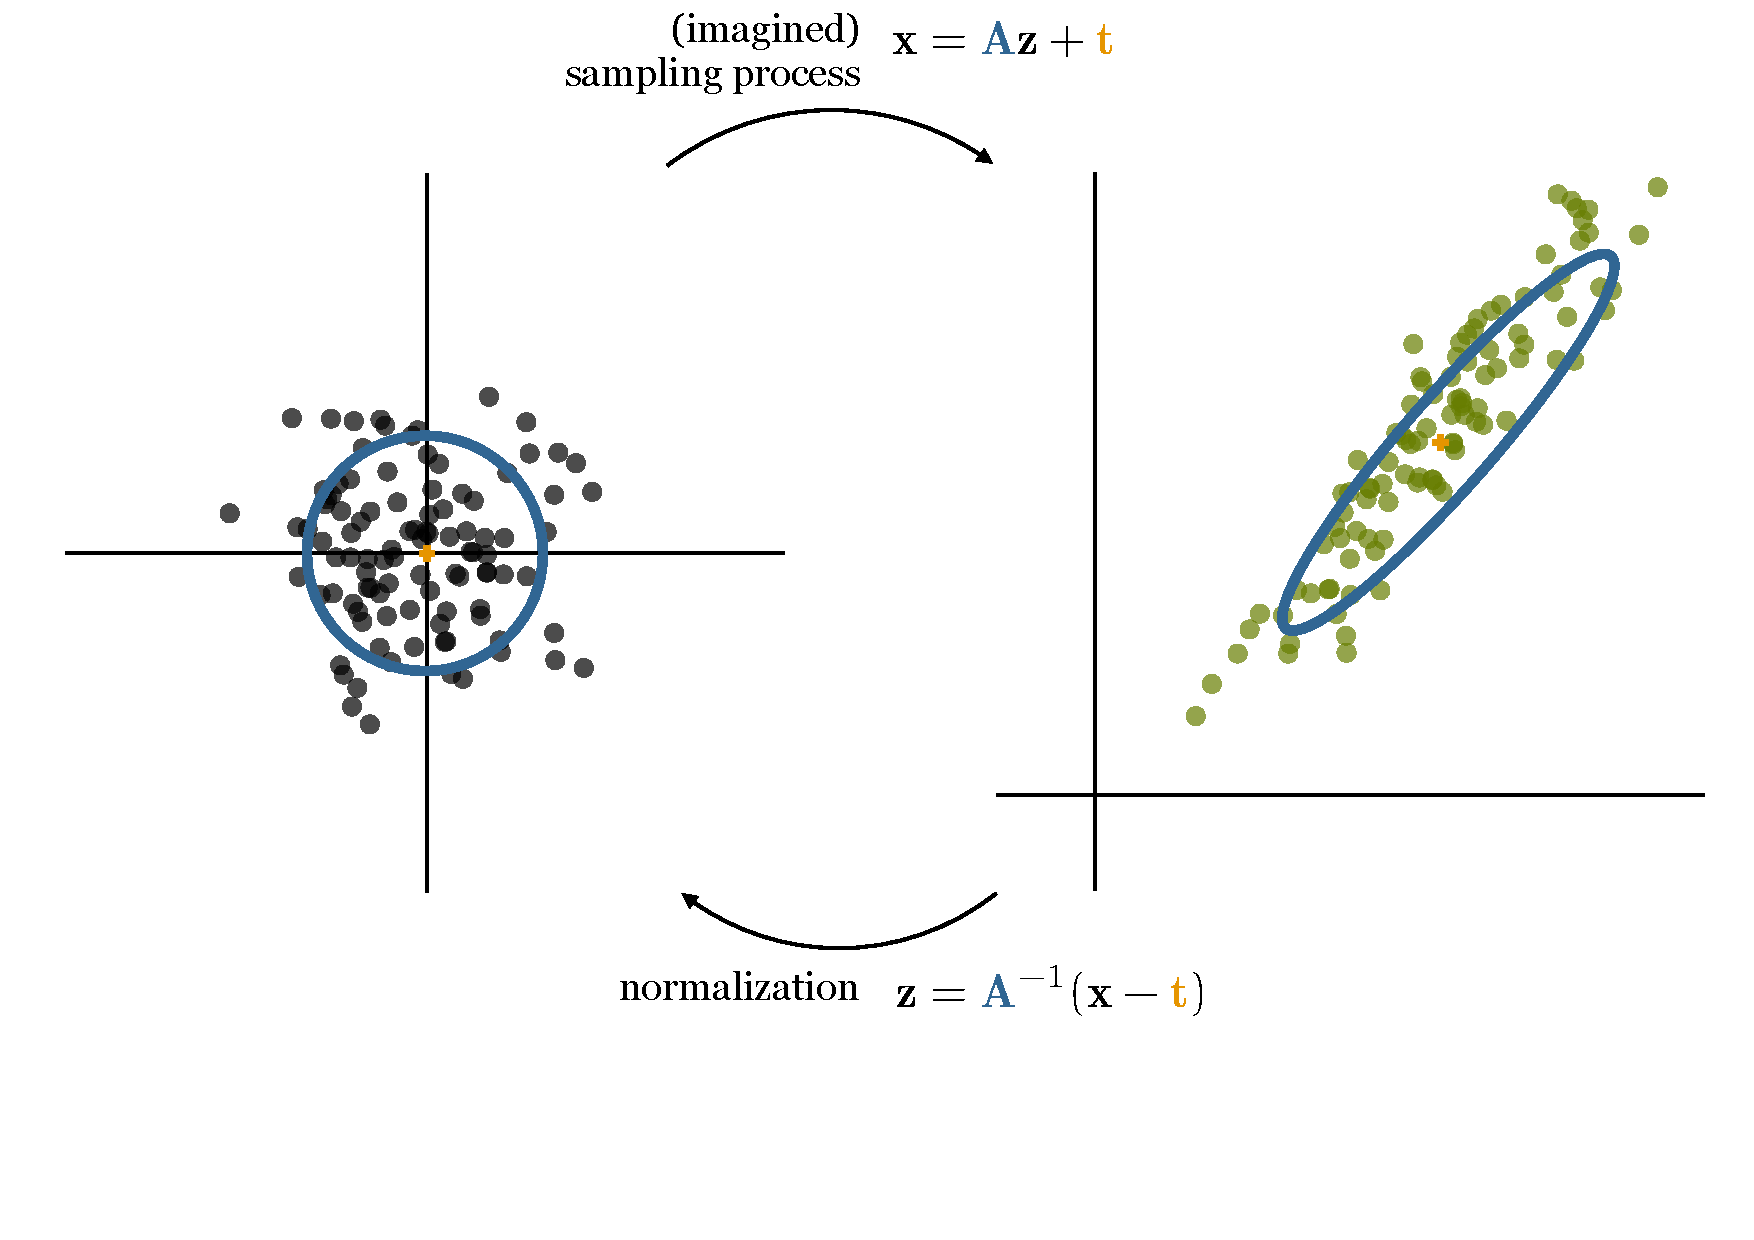
\includegraphics[width=0.85\textwidth]{./images/pca-4/normalization.pdf}}
	\caption*{Summary of normalization. We imagine some linear process has transformed the data from some standard-normally distributed data, and we invert that transformation. The \bc{sphere} of all unit vectors in the ``original'' space is transformed into an ellipse in the space of the data we observed.}
\end{figure}

%<figure class="centering narrow">
%<img src="/images/pca-4/normalization.svg"/>
%<figcaption>Summary of normalization. We imagine some linear process has transformed the data from some standard-normally distributed data, and we invert that transformation. The <span class="bc">sphere</span> of all unit vectors in the "original" space is transformed into an ellipse in the space of the data we observed.
%</figcaption>
%</figure>

What we saw in Chapter~\ref{chapter:eigenvectors}, is that if we can find \(\bc{\mbA}\) from the observed data, then the way in which \(\bc{\mbA}\) stretches space gives us the principal components of the data.

More specifically, imagine taking the (hyper)sphere of all unit vectors, and transforming them by \(\bc{\mbA}\). The result is an ellipsoid, and the major axis of this ellipsoid---the direction in which it bulges out the most---is the principal component of the data.


%<figure class="centering narrow">
%<img src="/images/pca-4/principal-axis.svg"/>
%<figcaption>Transforming the unit sphere by \(\bc{\A}\) results in an ellipse. Its <span class="rc"><em>major axis</em></span> is the direction in which it bulges out the most. In this view of the data, this direction is the first principal component.
%</figcaption>
%</figure>

\noindent We'll start with that intuition: \emph{the direction in which space is stretched the most by a transformation is important}, and see what it gets us when we apply it to general matrices.

Note that this is \emph{not} an eigenvector of \(\bc{\mbA}\) (It's an eigenvector of the covariance \(\bc{\mbS} = \bc{\mbA}^T\bc{\mbA}\), but we'll get to that later). An eigenvector of \(\bc{\mbA}\) is a vector whose direction doesn't change when multiplied by \(\bc{\mbA}\). This is different, in general, from the direction in which the transformation has the greatest effect.


\begin{figure}[H]
	\centerline{
		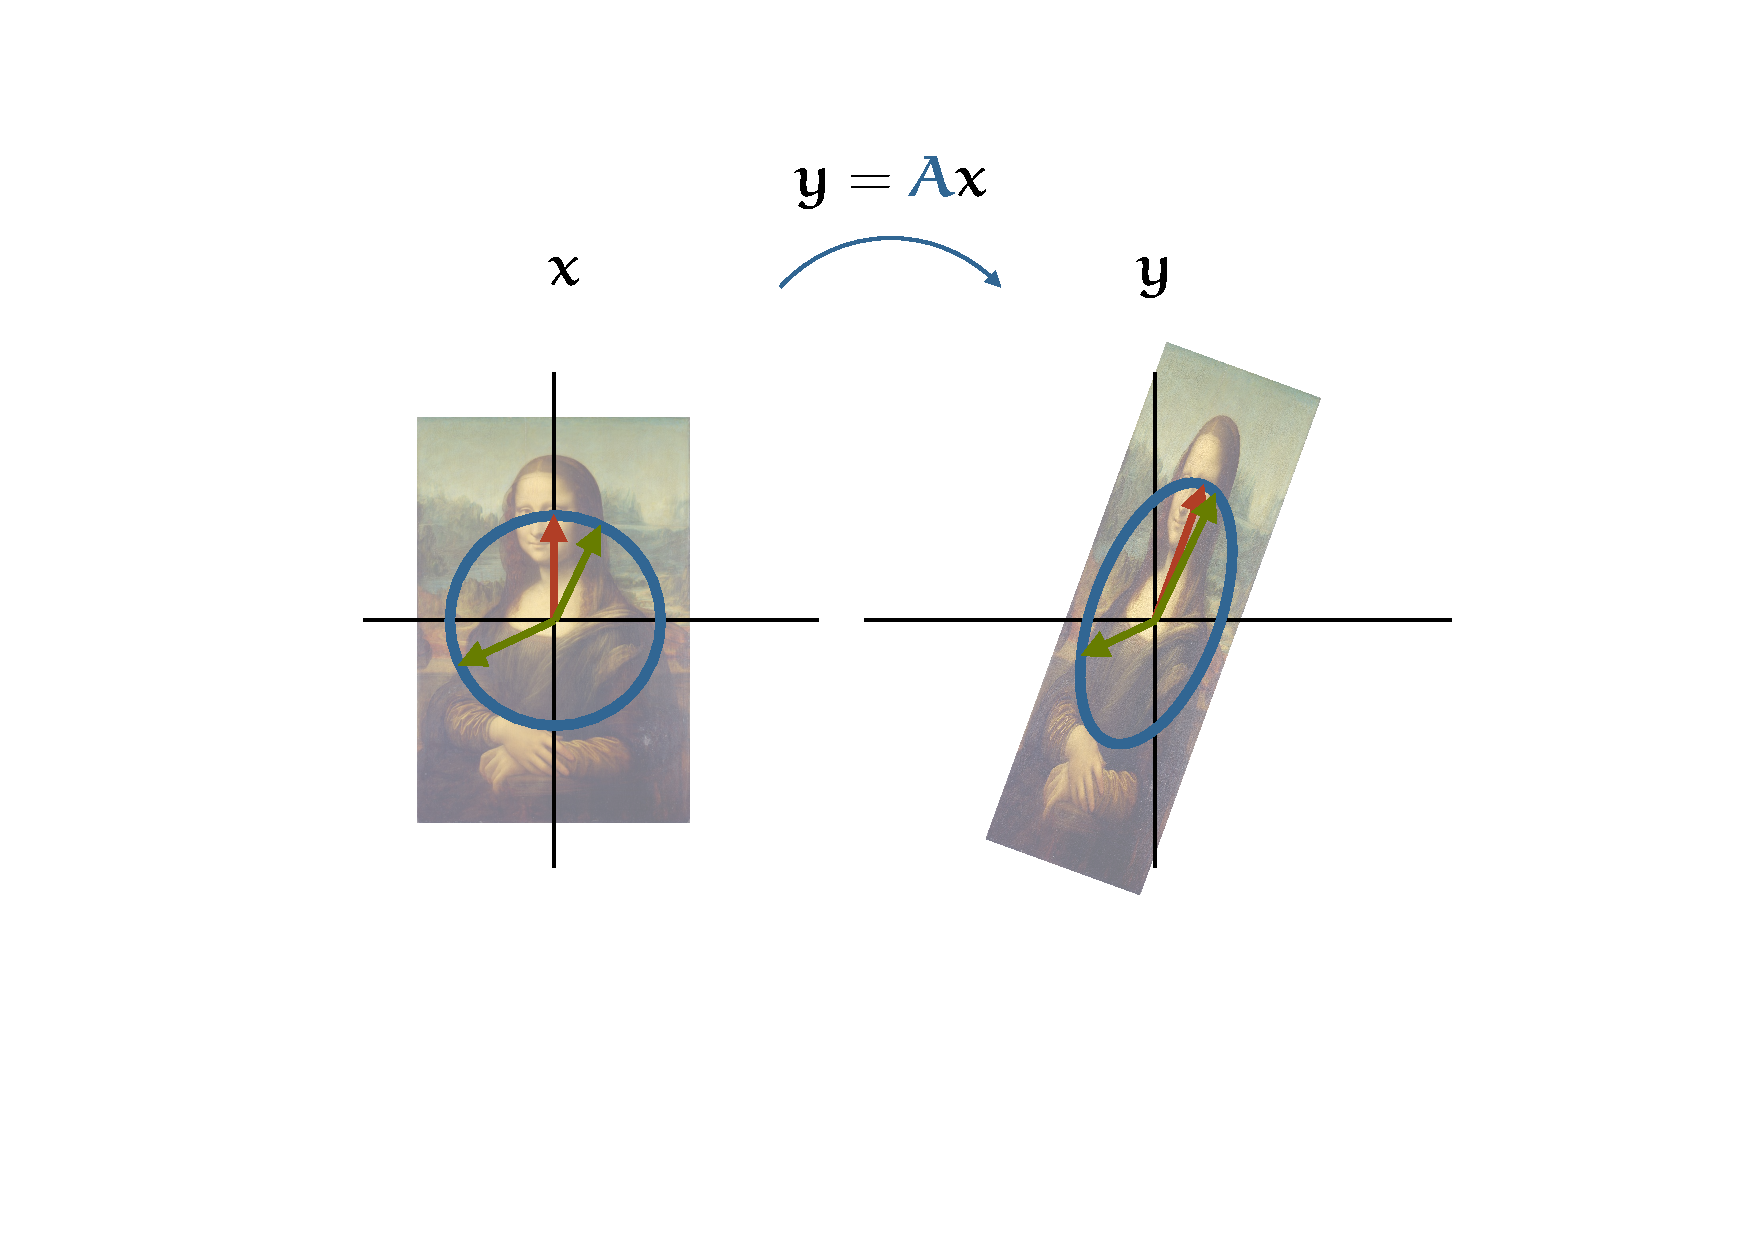
\includegraphics[width=0.8\textwidth]{./images/pca-4/eigvssing.pdf}
	}
	\caption*{The \rc{vector that is stretched the most by the transformation} is different from \gc{the eigenvectors}, which are vectors that don't change direction under the transformation.}
\end{figure}

\index{Vector of greatest stretch}

%<figure class="centering narrow">
%<img src="/images/pca-4/eigvssing.svg"/>
%<figcaption>The <span class="rc">vector that is stretched the most by the transformation</span> is different from <span class="gc">the eigenvectors</span>, which are vectors that don't change direction under the transformation. 
%</figcaption>
%</figure>

\begin{aside}If you are wondering why the eigenvectors in the image above aren't orthogonal to each other it's because the transformation matrix isn't symmetric, so the spectral theorem doesn't apply. It has two real eigenvalues, but not with orthogonal eigenvectors.
\end{aside}

We can now define the rest of the axes of our resulting ellipsoid in the same way we did with the principal components: for the second axis, we constrain it to be orthogonal to the first, and then see in which direction \(\bc{\mbA}\) causes the greatest stretch. For the third, we constrain it to be orthogonal to the first and second, and so on.

\enlargethispage{13.5pt}

\pagebreak
\noindent In this fashion, we get a series of vectors of ``greatest stretch'' that are all orthogonal to each other. 

The reason we are revisiting these intuitions is that \textbf{they still hold if \(\bc{\mbA}\) isn't square}. If we allow any matrix, including non-square ones, we can still carry this particular intuition over from the principal components. Let \(\gc{\mbM}\) be any matrix, with dimensions \(n \times m\). The multiplication

\[
\mby = \gc{\mbM} \mbx
\]

maps a vector \(\mbx \in \mR^m\) to a vector \(\mby \in \mR^n\). If we constrain \(\mbx\) to be a unit vector, then the possible inputs form a (hyper)sphere in \(\mR^m\). This sphere is mapped to an ellipsoid in \(\mR^n\). We don't need to know all the details about what ellipsoids are, just the basics: they are linear transformations of spheres, and the \emph{axes} of the ellipsoid are the directions where it bulges the most (with the second axis the biggest bulge orthogonal to the first, and so on).

For some matrices, for instance singular square ones, the resulting ellipsoid is not fully \(n\)-dimensional, but of some lower dimensionality. For instance, if \(m = n = 3\), there are matrices that produce a 2d ellipse, or even a 1d ellipsoid (a line segment). The matrix could even compress everything into a single point, which we'll call a 0d ellipsoid.

\index{Ellipsoid}

\begin{figure}[H]
	\centerline{
		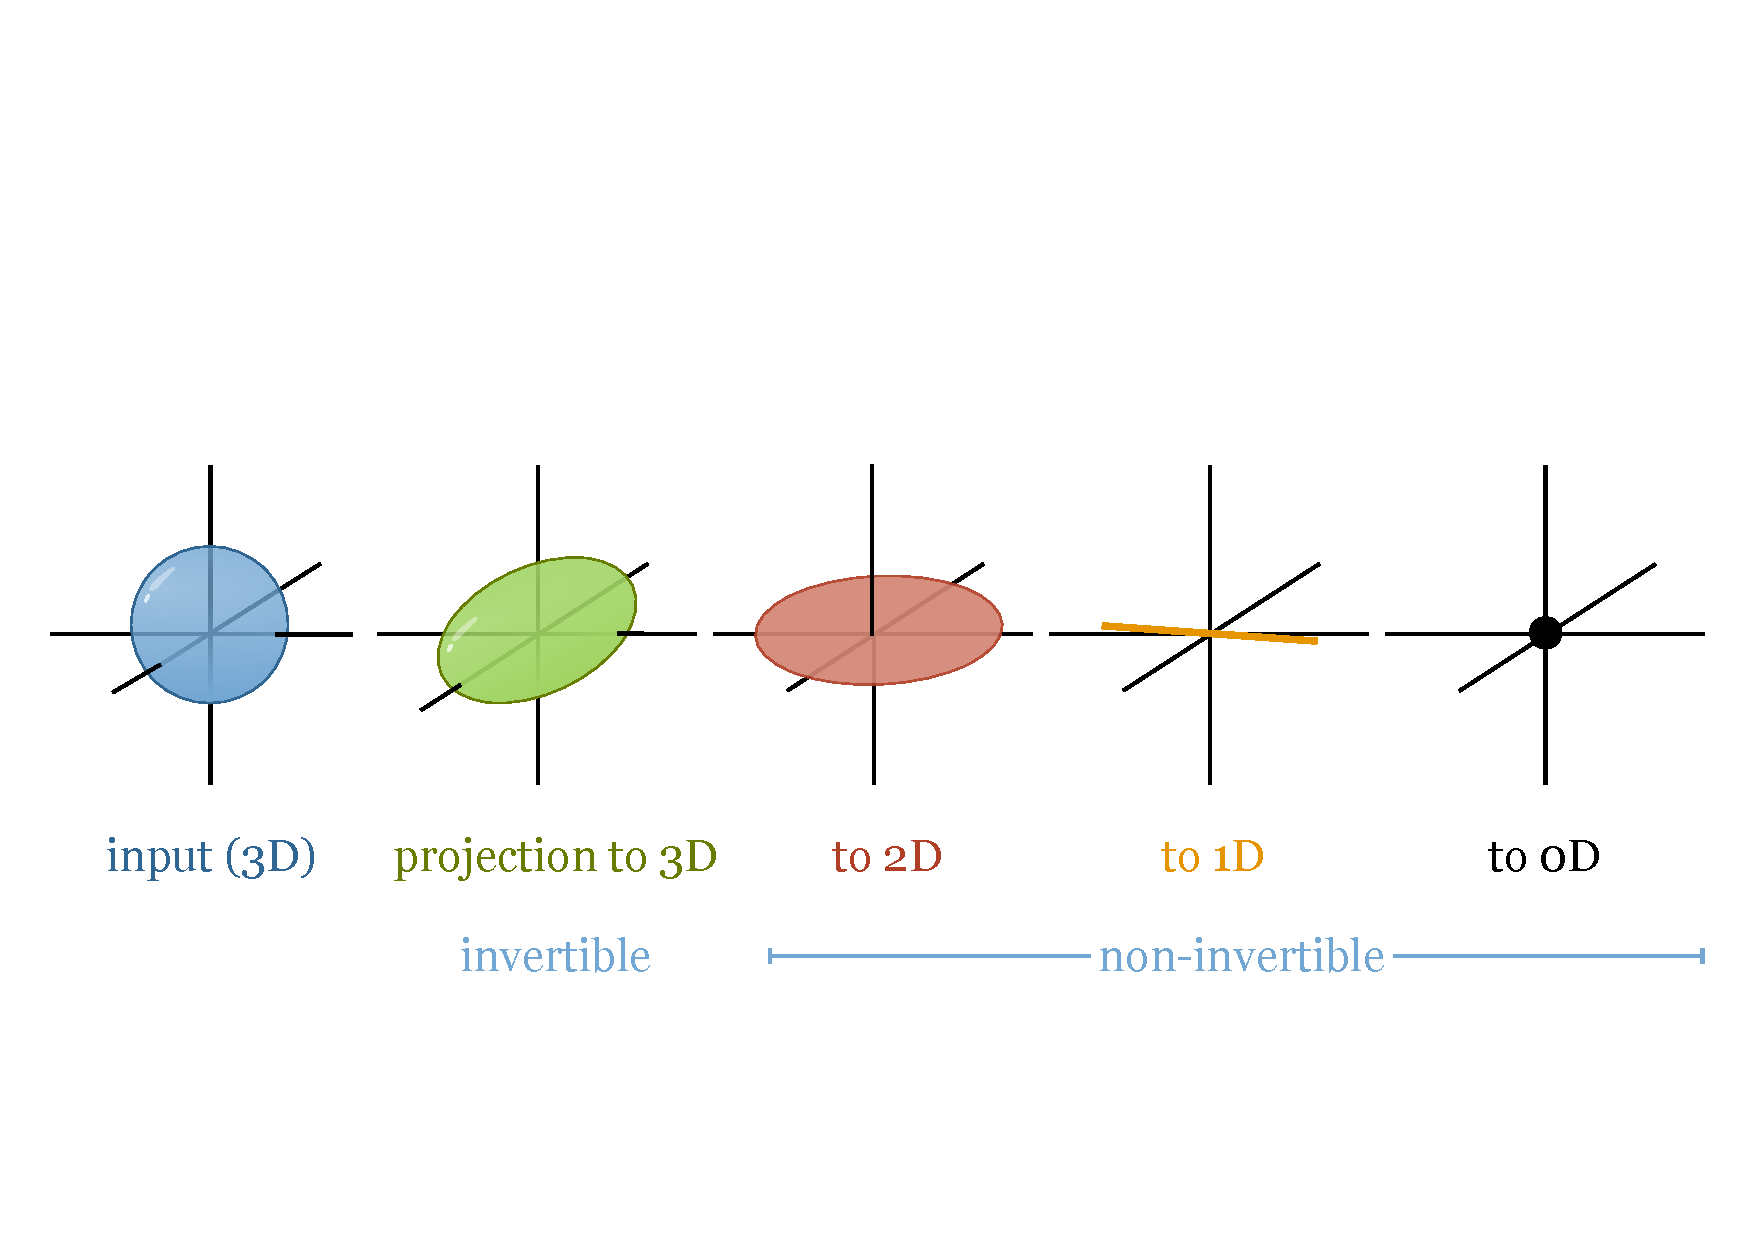
\includegraphics[width=1\textwidth]{./images/pca-4/ellipsoids.pdf}
	}
\end{figure}

%<figure class="narrow centering">
%<img src="/images/pca-4/ellipsoids.svg"/>
%</figure>

The same is true for matrices where \(n\) is bigger than \(m\), for instance a \(3 \times 2\) matrix. No linear transformation will turn a 2d sphere into a 3d ellipsoid, so the ellipsoid we get from a \(3 \times 2\) matrix must be at most 2 dimensional.

\begin{aside}We can put this more precisely when we've discussed matrix \emph{rank}.
\end{aside}

Nevertheless, the output is always an ellipsoid of some dimension, so our intuition carries over. We can always ask in which direction the resulting ellipsoid bulges out the most. It's just that after a few directions, the remainder may all be compressed to \(0\). For now, let's see what we can say about the directions that aren't.

So, the question is which unit vector is stretched the most by our matrix \(\gc{\mbM}\)? we can state this as an optimization problem:

\begin{align*}
\argmax{\mbx}      &\;\;  \|\gc{\mbM}\mbx\| \\
\text{such that} &\;\;  \|\mbx\| = 1 \p
\end{align*}

This problem simply asks for the input \(\mbx\) for which the resulting vector \(\gc{\mbM}\mbx\) has maximal magnitude, subject to the constraint that \(\mbx\) is a unit vector.

To find a solution to this problem, we can rewrite both norms as dot products. In the constraint, we know that setting the norm equal to 1 is the same as setting the dot product \(\mbx^T\mbx\) equal to 1. In the optimization objective, the norm and the dot product \emph{aren't} the same value (one is the square root of the other), but they \emph{are} maximized at the same \(\mbx\). So, we get the equivalent problem:

\begin{align*}
\argmax{\mbx}      &\;\; \mbx^T\gc{\mbM}^T\gc{\mbM}\mbx \\
\text{such that} &\;\; \mbx^T\mbx = 1 \p
\end{align*}

Something quite exciting has happened here. By one simple rewriting step, the maximum of the linear function \(\gc{\mbM}\mbx\) has become the maximum of the \emph{quadratic} function \(\mbx^T\bc{\mbS}\mbx\), with \(\bc{\mbS} = \gc{\mbM}^T\gc{\mbM}\).

\index{Quadratic function}

This is similar to what we derived in Chapter~\ref{chapter:eigenvectors}: there, we started with a (square) transformation matrix \(\bc{\mbA}\), which took our imagined standard-normally distributed data into the form we observed. We showed that \(\bc{\mbA}\) could be derived from the covariance matrix \(\kc{\frac{1}{n}}\mbX^T\mbX\) by the relation \(\bc{\mbA}\bc{\mbA}^T = \kc{\frac{1}{n}}\mbX^T\mbX\), and that optimizing for the direction of maximum stretch under \(\bc{\mbA}\) corresponds to the direction in which the quadratic form \(\mbx^T\left(\bc{\mbA\mbA}^T\right)\mbx\) is maximized.

\pagebreak

\noindent Most importantly, we saw there that maximizing the value \(\mbx^T\bc{\mbS}\mbx\) gives us the first eigenvector of \(\bc{\mbS}\). What we are seeing here is that the same thing holds for any matrix \(\gc{\mbM}\). Optimizing for maximum stretch gives us a direction that is equal to the first eigenvector \(\rc{\mbv}\) of \(\gc{\mbM}^T\gc{\mbM}\). Using this we can work out the relation between the amount that \(\rc{\mbv}\) is stretched in the multiplication \(\gc{\mbM}\rc{\mbv}\), and the corresponding eigenvalue of \(\gc{\mbM}^T\gc{\mbM}\):

\[
\|\gc{\mbM}\rc{\mbv}\|^2 = \rc{\mbv}^T\gc{\mbM}^T\gc{\mbM}\rc{\mbv} = \rc{\mbv}^T\bc{\lambda}\rc{\mbv} = \bc{\lambda}\rc{\mbv}^T\rc{\mbv} = \bc{\lambda} \p
\]

That is, if \(\rc{\mbv}\) is an eigenvector of \(\gc{\mbM}^T\gc{\mbM}\) with eigenvalue \(\bc{\lambda}\), then multiplying \(\rc{\mbv}\) by \(\gc{\mbM}\) stretches \(\rc{\mbv}\) by \(\sqrt{\bc{\lambda}}\).
%
Moreover, even though \(\gc{\mbM}\) may be non-square or singular, we know that \(\gc{\mbM}^T\gc{\mbM}\) is \emph{always} symmetric, which tells us that it has exactly \(m\) real eigenvalues, including multiplicities. The square roots of these eigenvalues indicate how much \(\gc{\mbM}\) stretches space along the various axes of the ellipsoid we get if we transform the unit vectors by it.

We call these values the \textbf{singular values} of \(\gc{\mbM}\). For each singular value \(\gc{\sigma}\), we have used two vectors in its definition. The unit vector \(\rc{\mbv} \in \mR^m\) which we multiplied by \(\gc{\mbM}\) and the vector that resulted from the multiplication. The latter has length \(\gc{\sigma}\) so we can represent it as \(\gc{\sigma}\rc{\mbu}\), where \(\rc{\mbu} \in \mR^n\) is also unit vector. With this, we can make our definition of the singular vectors similar to that of the eigenvectors: if \(\gc{\sigma}\) is a singular value of \(\gc{\mbM}\), then for its two singular vectors \(\rc{\mbv}\) and \(\rc{\mbu}\)

\index{Singular values|textbf}

\begin{align*}
\gc{\mbM}\rc{\mbv} &= \rc{\mbu}\gc{\sigma} \\
\end{align*}

We call \(\rc{\mbv}\) a \textbf{right singular vector} of \(\gc{\sigma}\) and \(\rc{\mbu}\) a \textbf{left singular vector}.

\index{Right singular vector}\index{Singular vector!right}
\index{Left singular vector}\index{Singular vector!left}

\begin{aside}We currently have the right singular vectors on the left and vice versa, which I admit is confusing, but they will change place as we develop a more complete definition.\end{aside}

You may ask what happens if an eigenvalue of \(\gc{\mbM}^T\gc{\mbM}\) is negative. We know that all eigenvalues are real, but we don't know that they are all positive. And we've defined the corresponding singular values as their square roots.

\index{Negative eigenvalues!of \(\gc{\mbM}^T\gc{\mbM}\)}

So, does the corresponding singular value of \(\gc{\mbM}\), become undefined, or complex? The answer is that we can prove that this doesn't happen. Note that if we pass a unit eigenvector \(\rc{\mbv}\) of \(\bc{\mbA}\) into its quadratic \(\rc{\mbv}^T\bc{\mbA}\rc{\mbv}\), the result is its eigenvalue \(\rc{\mbv}^T\bc{\lambda}\rc{\mbv} = \bc{\lambda} \kc{\mbv^T\mbv}\). Now, let \(\mby = \gc{\mbM}\mbx\). Then if \(\mbx\) is an eigenvector of \(\gc{\mbM}^T\gc{\mbM}\), the quadratic \(\mbx^T\gc{\mbM}^T\gc{\mbM}\mbx = \mby^T\mby\) is the corresponding eigenvalue. This is simply the sum of the squared elements of \(\mby\). Whether these are positive or negative, the result is always nonnegative, which shows an eigenvalue of \(\gc{\mbM}^T\gc{\mbM}\) will always be non-negative.

\begin{aside}In technical terms, we have just shown that \(\gc{\mbM}^T\gc{\mbM}\) is \emph{positive semidefinite}.
\end{aside}

\index{Positive semidefinite matrix}

So, we can be sure that there are always \(m\) nonnegative singular values for \(\gc{\mbM}\), even though some of them may be zero.

\subsection{Singular vectors and principal components}

Before we develop the singular values and vectors further, let's see what their relevance is in the context of principal component analysis. In PCA, we start with a data matrix \(\mbX\), of size \(n \times m\), which arranges the \(n\) instances in our data along the rows, and the \(m\) features of each along the columnns.

We can ask what the singular values of \(\mbX\) are. You may be able to predict the answer, but first let's look at what how this squares with our intuition of singular values. We said that they represent the maximal amount multiplying a vector by \(\mbX\) stretches that vector. What does it mean to multiply a vector by the data matrix?

Let's take a vector \(\bc{\mbp} \in \mR^m\) (where \(m\) is the number of features in our data), and let's assume \(\bc{\mbp}\) is a unit vector. That way, we are limited in how big we can make each entry. Now multiply \(\mby = \mbX\bc{\mbp}\). We get a vector of length \(n\): one value for each instance \(\mbx\) in our data, which is the dot product of that instance and our vector \(\bc{\mbp}\). This value is high if the features of the instance match the corresponding values of \(\bc{\mbp}\) in magnitude and sign: they should be big where \(\bc{\mbp}\) is big and negative where \(\bc{\mbp}\) is negative.

\pagebreak
\noindent That is, the dot product expresses a kind of \emph{similarity} between \(\bc{\mbp}\) and the instances in our data. The elements of \(\mby\) tell us which instances in the data ``match'' \(\bc{\mbp}\) the best. This means that the vector \(\bc{\mbp}\) that is stretched the most by \(\mbX\), is the vector that is most similar to \emph{all instances}. This is a tradeoff: making it more similar to one instance may make it less similar to other instances. Balancing this over all instances, we get the direction that maximizes \(\|\mby\|\): the first singular vector of \(\mbX\).

If we assume that the data is mean-centered, we can imagine this direction pivoting around the origin, averaging the angles to all instances, proportional to how far from the origin each instance is. This should remind you of how we plotted the first principal component earlier.

\begin{figure}[H]
	\centerline{
		\includesvg[width=1\textwidth]{./images/pca/sol-w.svg}
	}
	\caption*{From Chapter~\ref{chapter:introduction}: the first PC for a simple dataset.
	}
\end{figure}

%<figure class="narrow">
%<img src="/images/pca/sol-w.svg">
%<figcaption>From <a href="">part one</a>: the principal component of a simple dataset.
%</figcaption>
%</figure>

It's not hard to prove that this direction of maximal stretch is indeed the first principal component. As we've seen the maximal direction is an eigenvector of the matrix \(\mbX^T\mbX\). What we also saw, in Chapter~\ref{chapter:eigenvectors}, is that the covariance matrix is estimated with \(\kc{\frac{1}{n}}\mbX^T\mbX\).

The constant factor \(\kc{\frac{1}{n}}\) doesn't really matter much for our purposes. If we diagonalize \(\mbX^T\mbX\) as \(\rc{\mbP}^T\bc{\mbD}\rc{\mbP}\), then we can write \(\rc{\mbP}^T\kc{\frac{1}{n}}\bc{\mbD}\rc{\mbP}\) for the properly normalized covariance. In other words \(\mbX^T\mbX\) and \(\kc{\frac{1}{n}}\mbX^T\mbX\) have the same eigenvectors, and their eigenvalues only differ by a multiplicative constant \(\kc{\frac{1}{n}}\).

Thus, the directions corresponding to the singular values of \(\mbX\) are the same as the eigenvectors of the covariance matrix. We've already established that the singular values of \(\mbX\) are the square roots of the corresponding eigenvalues of \(\mbX^T\mbX\), so we can say that they are proportional to the eigenvalues of \(\bc{\mbS}\).

We can now show that the singular values and eigenvalues are in some sense generalizations of standard deviation and variance. To illustrate, assume that our data \(\mbX\) is one-dimensional. In this case, we could estimate the variance with the formula:

\[
\text{var } \mbX =  \kc{\frac{1}{n}} \sum_i {X_{i1}}^2
\]

which we can also write as

\[
\kc{\frac{1}{n}} \mbX^T\mbX = \mbX'^T\mbX'
\]
with \(\mbX' = \kc{\frac{1}{\sqrt{n}}} \mbX\).

In this case \({\mbX'}^T\mbX'\) has one eigenvalue, which is simply the scalar value \({\mbX'}^T\mbX'\). As shown above, this corresponds to the estimated variance of the data. The corresponding \emph{singular} value of \(\mbX'\) is its square root: the standard deviation.

In short, if we ignore a scaling factor of \(\frac{1}{\sqrt{n}}\), the singular values of \(\mbX\) are analogous to the standard deviation and the eigenvalues of the covariance matrix \(\mbX^T\mbX\) are analogous to the variance.

\index{Variance}\index{Standard deviation}
\index{Eigenvalues!analogy to variance}\index{singular values!analogy to standard deviation}

\subsection{The singular value decomposition}

When we developed eigenvalues and eigenvectors, we saw that they allowed us to decompose square matrices as the product of three simpler matrices: \(\bc{\mbA} = \rc{\mbP}\bc{\mbD}\rc{\mbP}^T\). We can do the same thing with singular values and vectors.

We've seen that any matrix has \emph{singular values}, which correspond to two kinds of singular \emph{vectors}, defined in a way that is similar to the way eigenvectors are defined. Here, we have the eigenvalue definition on the left and the singular value definition on the right

\[
\bc{\mbA}\rc{\mbw} = \rc{\mbw}\bc{\lambda} \hspace{10em} \gc{\mbM}\rc{\mbv} = \rc{\mbu}\gc{\sigma} \p
\]

From the definition of the eigenvalue and vector, we managed to construct a decomposition of \(\bc{\mbA}\). 

\pagebreak
\noindent A straightforward way to do this is the following recipe.
\begin{enumerate}
\item Assume that the \(n \times n\) matrix \(\bc{\mbA}\) has \(n\) real eigenvalues \(\bc{\lambda}_i\), with unit eigenvectors \(\rc{\mbw}_i\).
\item Arrange the eigenvectors as columns of a matrix so that we get \(\bc{\mbA}\left[\rc{\mbw}_1 \ldots \rc{\mbw}_n\right] = \left[\rc{\mbw}_1\bc{\lambda}_1 \ldots \rc{\mbw}_n\bc{\lambda}_n\right]\)
\item Let \(\rc{\mbP} = \left[\rc{\mbw}_1 \ldots \rc{\mbw}_n\right]\) and \(\bc{\mbD} = \text{diag}(\bc{\lambda}_1 \ldots \bc{\lambda}_n)\) so that \(\bc{\mbA}\rc{\mbP} = \rc{\mbP}\bc{\mbD}\)
\item Note that \(\rc{\mbP}\) is orthogonal, so that \(\bc{\mbA} = \rc{\mbP}\bc{\mbD}\rc{\mbP}^T\)
\end{enumerate}

\index{Eigendecomposition!recipe}

The fact that the eigenvectors are orthogonal comes from the iterative way in which we chose them: each was chosen to be orthogonal to all the previous choices. We did the same for the singular vectors. The assumption that we have \(n\) real eigenvalues comes from the spectral theorem.

One thing we haven't examined yet in any detail, is what happens if our eigenvectors are zero. This can happen if we have a square, symmetric matrix which is non-invertible, like 

\[
\begin{pmatrix} 1 & \kc{0}\\ \kc{0}& \kc{0} \end{pmatrix} \p
\]

In such cases, we get one or more \(\bc{0}\) eigenvalues. What are the corresponding eigenvectors? In many ways it doesn't matter: the defining relation \(\bc{\mbA}\rc{\mbw} = \rc{\mbw}\bc{0}\) always holds, whatever \(\rc{\mbw}\) we choose. To make the above recipe work, all we need to do is to choose \(\rc{\mbw}\) so that it is a unit vector, and orthogonal to any \(\rc{\mbw}\) we already chose. 

If we try to follow the same recipe with the singular vectors, we might get something like this.

\begin{enumerate}
\item Assume that the \(n \times m\) matrix \(\gc{\mbM}\) has \(k\) singular values \(\gc{\sigma}_i\), with unit left and right singular vectors \(\rc{\mbu}_i \in \mR^n\) and \(\rc{\mbv}_i\in \mR^m\).

\item Arrange the singular vectors as columns of matrices so that we get \(\gc{\mbM}\left[\rc{\mbv}_1 \ldots \rc{\mbv}_k\right] = \left[\rc{\mbu}_1\gc{\sigma}_1 \ldots \rc{\mbu}_k\gc{\sigma}_k\right]\).

\item Let \(\rc{\mbV} = \left[\rc{\mbv}_1 \ldots \rc{\mbv}_k\right]\), \(\rc{\mbU} = \left[\rc{\mbu}_1 \ldots \rc{\mbu}_k\right]\) and \(\gc{\Sig} = \text{diag}(\gc{\sigma}_1 \ldots \gc{\sigma}_k)\) so that \(\gc{\mbM}\rc{\mbV} = \rc{\mbU}\gc{\Sig}\).
\end{enumerate}

This is as far as we get. There aren't necessarily sufficient singular values to ensure that \(\rc{\mbV}\) is square. That means \(\rc{\mbV}\) is not invertable, so we can't take it to the other side of the equation.

\begin{aside}
We have \(\rc{\mbV}^T\rc{\mbV} = \mbI\), but to take \(\rc{\mbV}\) to the other side, we'd need \(\rc{\mbV}\rc{\mbV}^T = \mbI\), which we only get if \(\rc{\mbV}\) is square.
\end{aside}

A simple solution is to extend \(\rc{\mbV}\) to a complete basis. We know that the \(k\) singular vectors making up \(\rc{\mbV}\) are mutually orthogonal, and we know that we can always choose \(m - k\) additional unit vectors orthogonal to these and to each other. If we add them to \(\rc{\mbV}\) as columns, \(\rc{\mbV}\) becomes an \(m \times m\) orthonormal matrix.

\index{Orthogonal basis}

If we add one such vector \(\rc{\mbv}'\) to \(\rc{\mbV}\), what do we need to change to keep our equation \(\gc{\mbM}\left[\rc{\mbv}_1 \ldots \rc{\mbv}_k\right] = \left[\rc{\mbu}_1\gc{\sigma}_1 \ldots \rc{\mbu}_k\gc{\sigma}_k\right]\) intact? We need to extend the right with the vector \(\gc{\mbM}\rc{\mbv}'\). What can we say about this vector? First, we can always write any vector as a unit vector times a scalar length, so let's call it \(\rc{\mbu}'\gc{\sigma}'\). 

\[
\gc{\mbM}\left[\rc{\mbv}_1 \ldots \rc{\mbv}_k\; \rc{\mbv}'\right] = \left[\rc{\mbu}_1\gc{\sigma}_1 \ldots \rc{\mbu}_k\gc{\sigma}_k\; \rc{\mbu}'\gc{\sigma}'\right]
\]

Note that we assumed that we have all \(k\)  singular values of \(\gc{\mbM}\) already. This means that there is no vector \(\rc{\mbv}\) orthogonal to all \(\rc{\mbv}_i\) such that \(\|\gc{\mbM}\rc{\mbv}\| > 0\), or it would be a candidate for the \(k+1\)th singular vector. Therefore, \(\|\gc{\mbM}\rc{\mbv}'\| = 0\).

\begin{aside}\(\rc{\mbv}'\) is in the \emph{null space} of \(\gc{\mbM}\).\end{aside}

\index{Null space}

This means that we can set \(\gc{\sigma}' = 0\) and choose \(\rc{\mbu}'\) however we like. We will choose some vector that is orthogonal to all \(\rc{\mbu}_i\) already chosen.

\begin{aside}Note the similarity to the eigenvector case: once we've run out of nonzero singular values we extend the rest of the diagonal with zeros.
\end{aside}	

We could just keep adding vectors like this until \(\rc{\mbV}\) is square, and it would be orthogonal so we would be allowed to move it to the other side. But we'd be missing a trick if we stopped there. The matrix \(\gc{\mbM}\) represents a function from one space, \(\mR^m\) to another \(\mR^n\). If we make \(\rc{\mbV}\) square and orthogonal, we have constructed an orthonormal \emph{basis} for \(\mR^m\), just like the analogous \(\rc{\mbP}\) is a basis in the eigendecomposition. It would be quite nice, if we could ensure that \(\rc{\mbU}\) is also an orthonormal basis for \(\mR^n\). That way, we would have two orthonormal bases \(\rc{\mbU}\) and \(\rc{\mbV}\) for the two spaces that \(\gc{\mbM}\) transforms between, and a diagonal matrix of singular \(\gc{\Sig}\) values in the middle.

\index{Orthogonal matrix}\index{Orthonormal basis}

To do this, we need to add different numbers of orthogonal vectors to \(\rc{\mbV}\) and \(\rc{\mbU}\). \(\rc{\mbV}\) needs \(k-m\) extra vectors to become \(m \times m\), and \(\rc{\mbU}\) needs \(k-n\) extra vectors to become \(n \times n\). The trick to accomplish this is to make \(\gc{\Sig}\) \emph{non-square}. We make \(\gc{\Sig}\) an \(m \times n\) matrix, with all zeros except for the diagonal of the top \(k \times k\) matrix in the top left, which contains the singular values. Here is an illustration.

\begin{figure}[H]
	\centerline{
		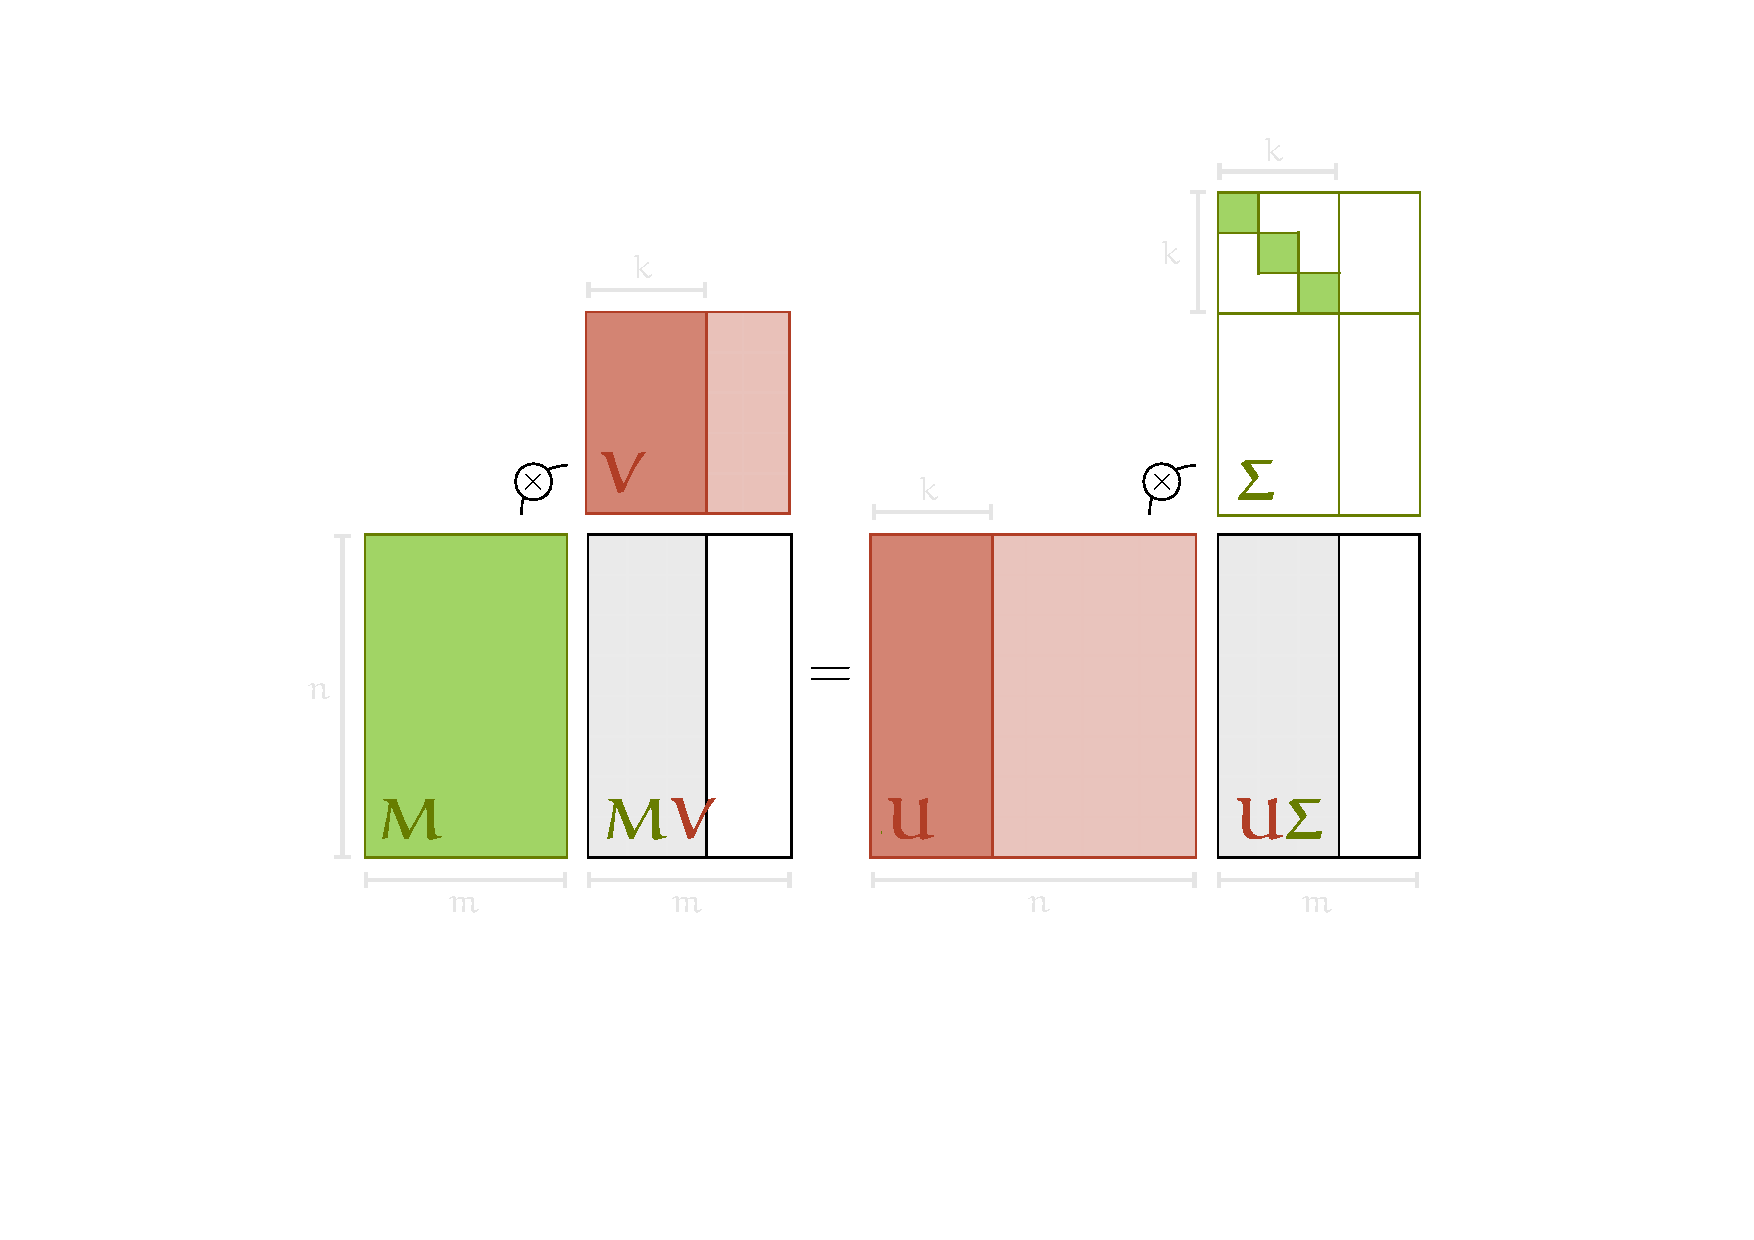
\includegraphics[width=1\textwidth]{./images/pca-4/svd-multiplication.pdf}
	}
	\caption*{Diagram for the equation \(\gc{\mbM}\rc{\mbV} = \rc{\mbU}\gc{\Sig}\). White cells represent \(0\)s. The light columns of \(\rc{\mbV}\) and \(\rc{\mbU}\) are the vectors we add to make these matrices square.
	}
\end{figure}

%<figure class="narrow">
%<img src="/images/pca-4/svd-multiplication.svg">
%<figcaption>Diagram for the equation \(\gc{\M}\rc{\V} = \rc{\U}\gc{\Sig}\). White cells represent \(0\)s. The light columns of \(\rc{\V}\) and \(\rc{\U}\) are the vectors we add to make these matrices square.
%</figcaption>
%</figure>

We see that the effect of extending \(\rc{\mbV}\) with orthogonal vectors is to add zero columns to the product \(\gc{\mbM}\rc{\mbV}\). This is not surprising, since we noted already that these must be in the null space of \(\gc{\mbM}\).

\pagebreak \noindent On the right, the product \(\rc{\mbU}\gc{\Sig}\) needs to be equal to \(\gc{\mbM}\rc{\mbV}\). The extra zero columns can easily be added by adding zero columns to \(\gc{\Sig}\).

How about the extra basis vectors we would like to add to \(\rc{\mbU}\)? We need to add rows to \(\gc{\Sig}\) in order to make the matrix dimensions match. If the rows we add are zero rows, then we can be sure that when we multiply the two matrices, any entry in any column added to \(\rc{\mbU}\) will be multiplied by \(0\), so it won't affect the product \(\rc{\mbU}\gc{\Sig}\).

\pagebreak[3]

Here is the process in three steps:

\begin{figure}[H]

	\parbox[b]{.5\textwidth}{
    	\hspace{5mm}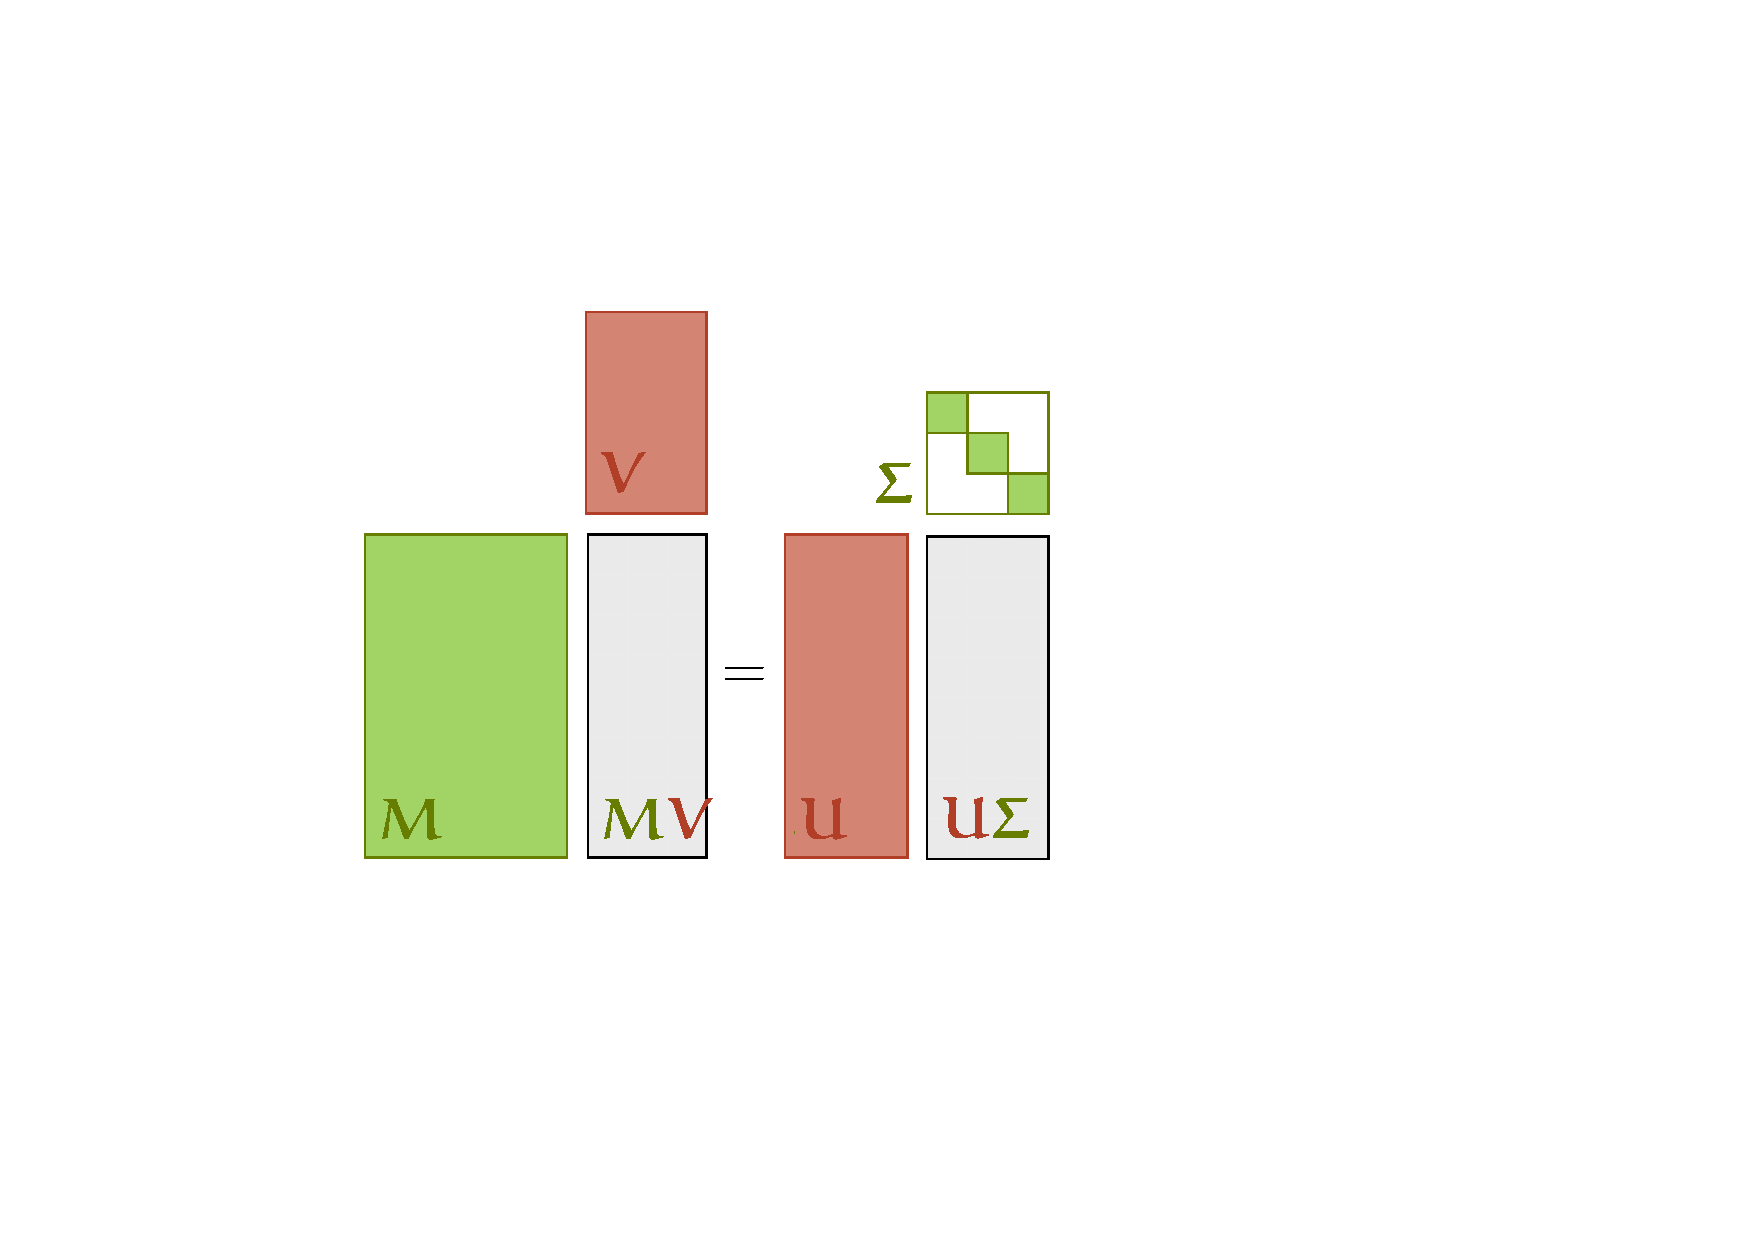
\includegraphics[width=0.5\textwidth]{./images/pca-4/svd-multiplication-step1.pdf}
	}\hspace{.0\textwidth}%
	\parbox[b]{.5\textwidth}{
		\caption*{Set up the singular values and vectors in a matrix multiplication.}
	}
	
	\parbox[b]{.5\textwidth}{
    	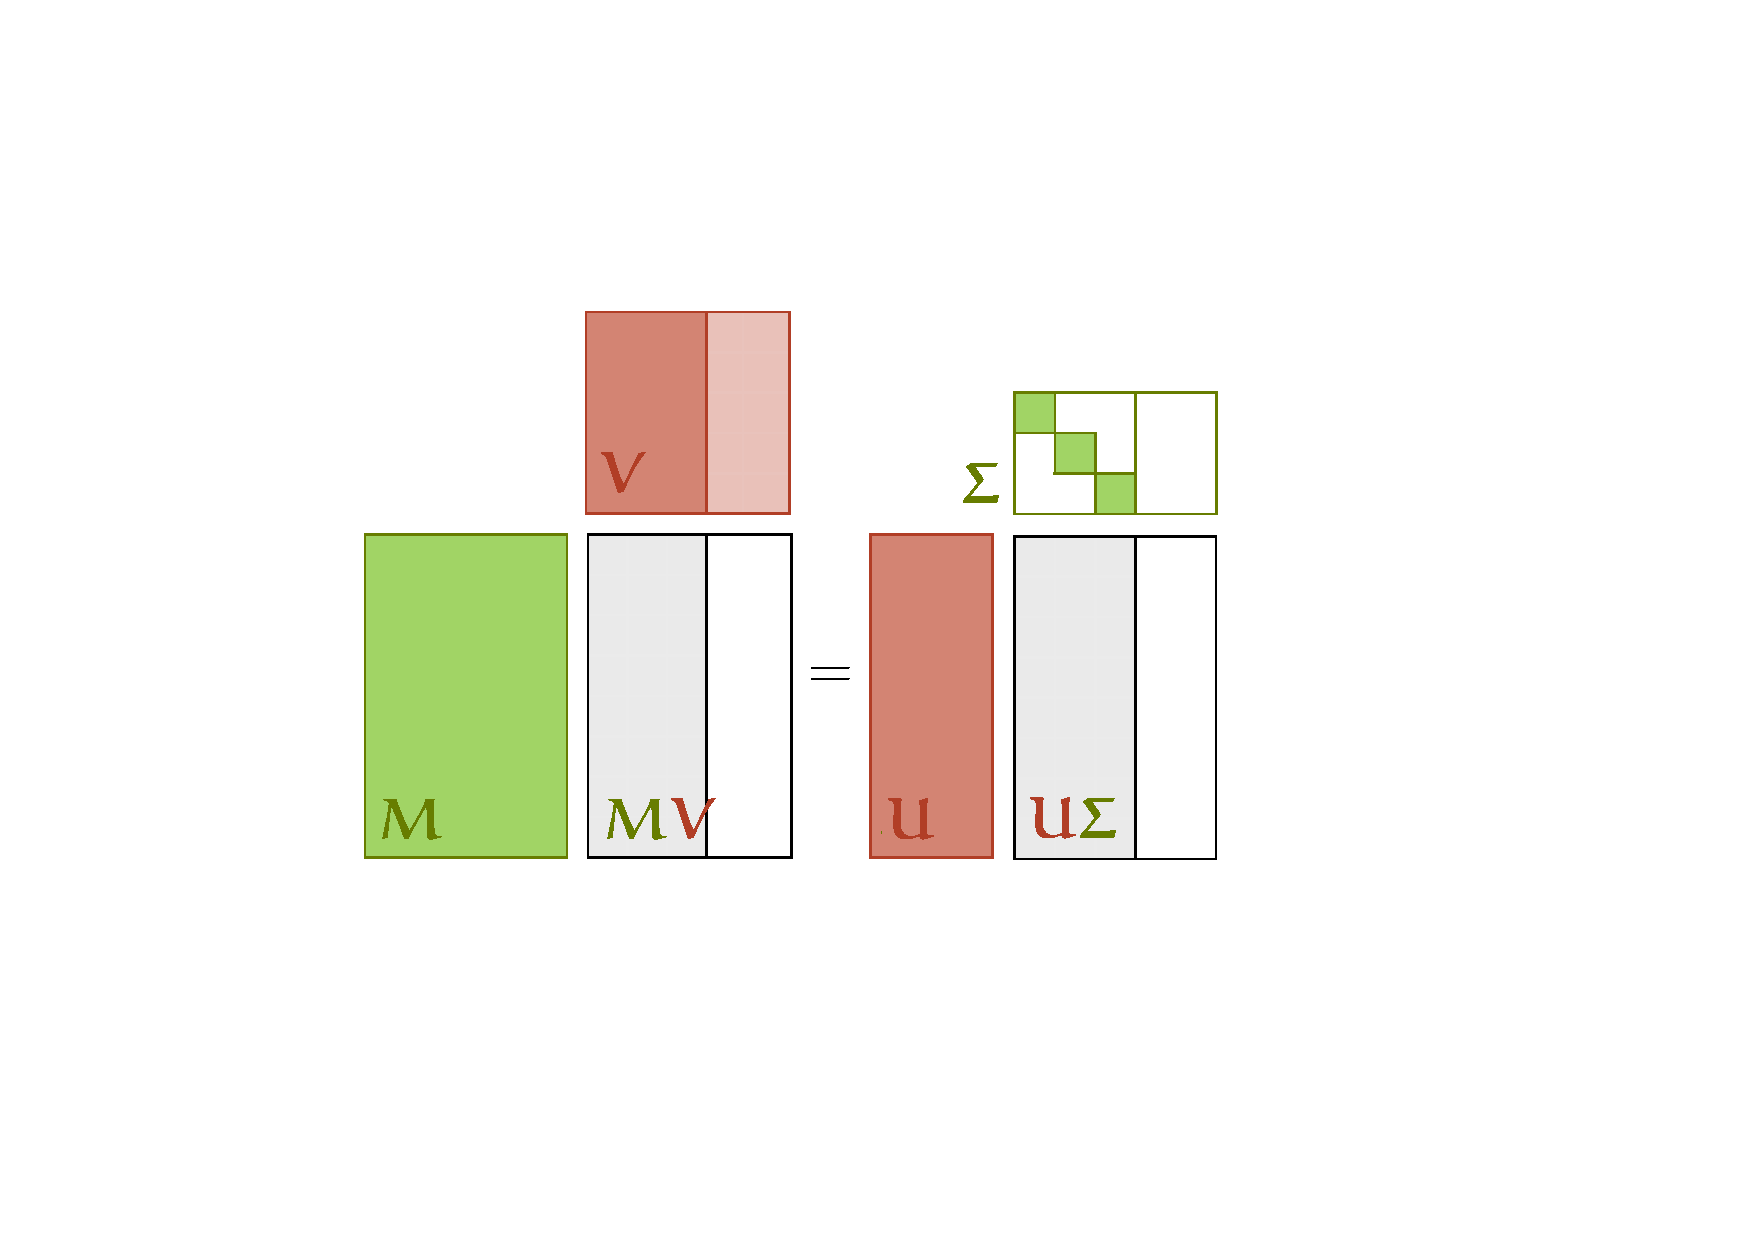
\includegraphics[width=0.5\textwidth]{./images/pca-4/svd-multiplication-step2.pdf}
	}\hspace{.0\textwidth}%
	\parbox[b]{.5\textwidth}{
		\caption*{Add orthogonal vectors to \(\rc{\mbV}\) to make it square. Add zero columns to \(\gc{\Sig}\) to make the sizes match.}
	}	
	
	\parbox[b]{.5\textwidth}{
    	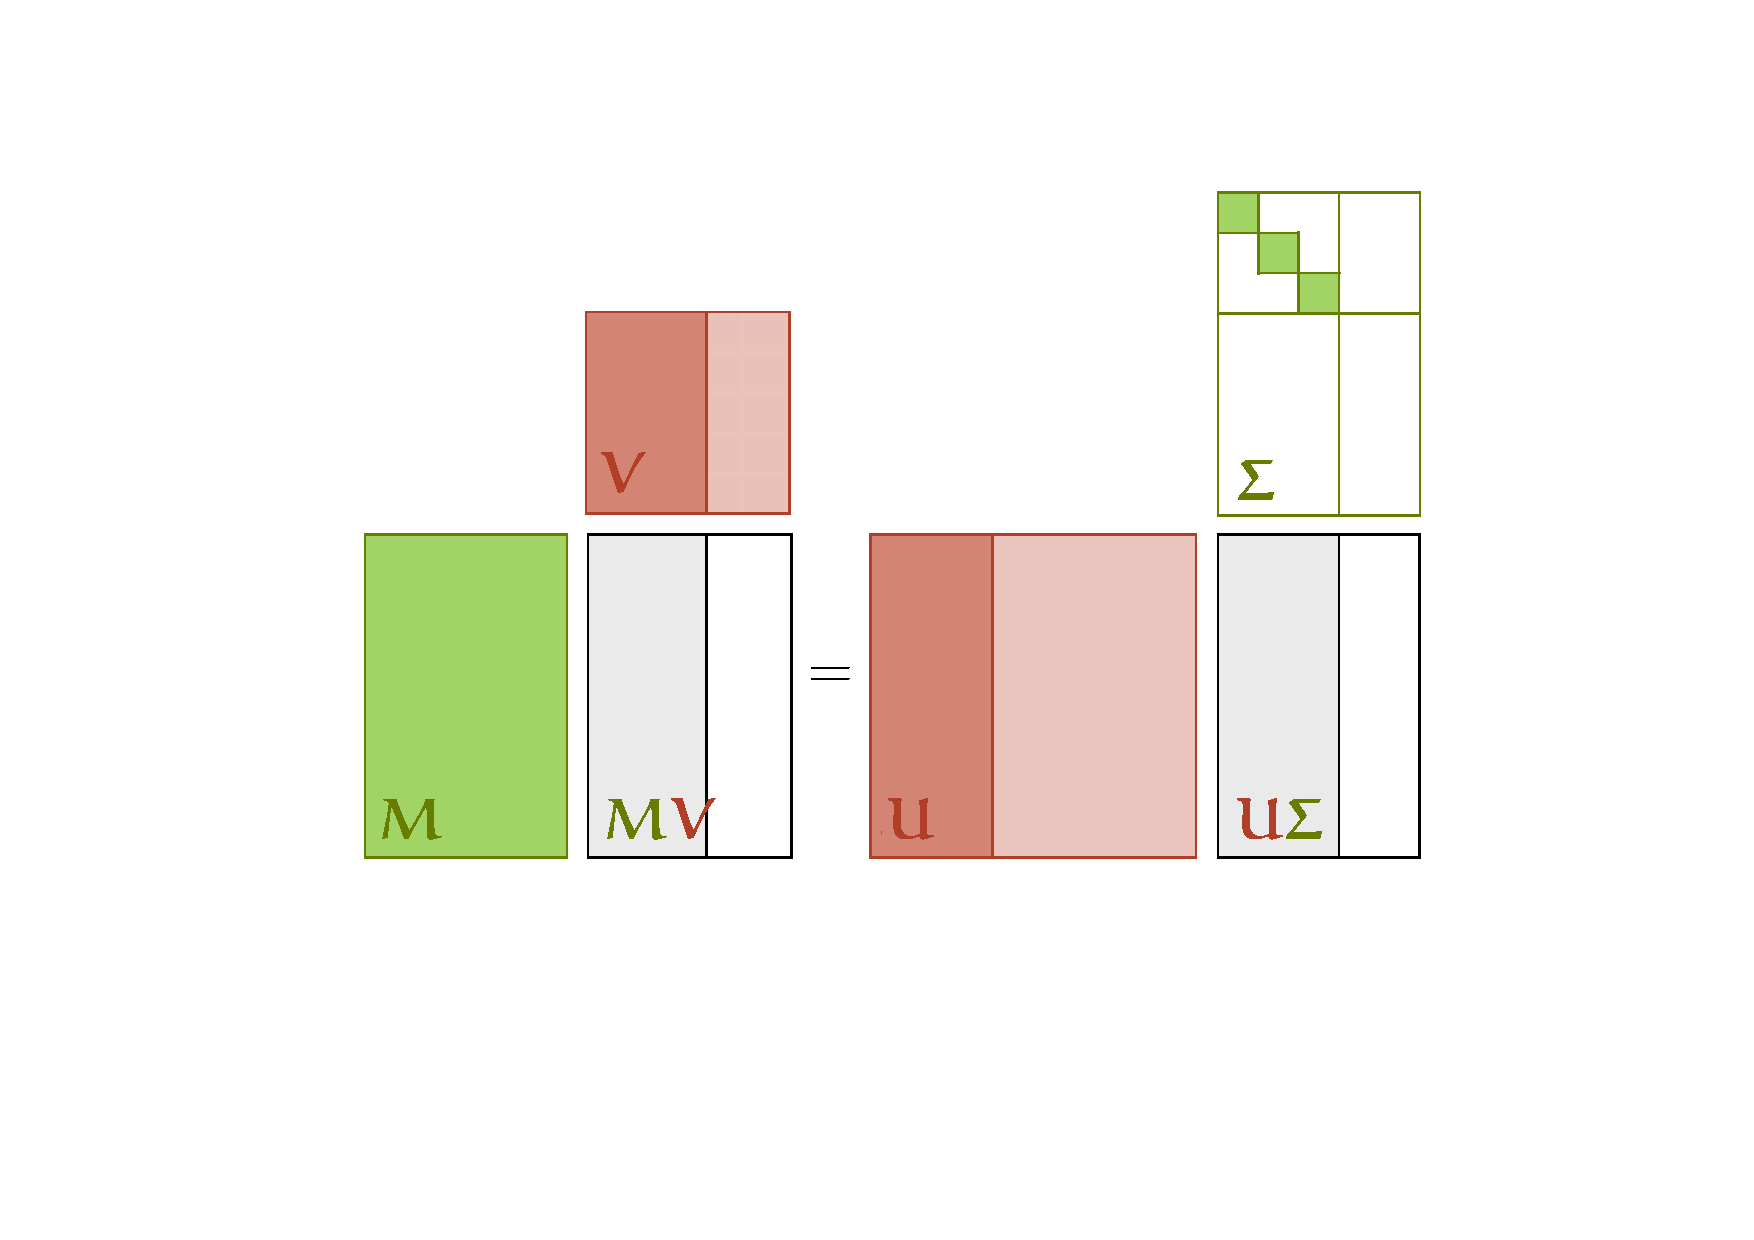
\includegraphics[width=0.5\textwidth]{./images/pca-4/svd-multiplication-step3.pdf}
	}\hspace{.0\textwidth}%
	\parbox[b]{.5\textwidth}{
		\caption*{Add orthogonal vectors to \(\rc{\mbU}\) to make it square. Add zero rows to \(\gc{\Sig}\) to make the sizes match.}
	}		
\end{figure}

\index{Singular value decomposition!recipe}
%<figure class="narrow steps">
%<img src="/images/pca-4/svd-multiplication-step1.svg"> 
%<figcaption>Set up the singular values and vectors in a matrix multiplication.</figcaption>
%
%<img src="/images/pca-4/svd-multiplication-step2.svg">
%<figcaption>Add orthogonal vectors to \(\rc{\V}\) to make it square. Add zero columns to \(\gc{\Sig}\) to make the sizes match.</figcaption>
%
%<img src="/images/pca-4/svd-multiplication-step3.svg">
%<figcaption>Add orthogonal vectors to \(\rc{\U}\) to make it square. Add zero rows to \(\gc{\Sig}\) to make the sizes match.</figcaption>
%</figure>

Now, we can safely take \(\rc{\mbV}\) to the other side (that is, multiply both sides by \(\rc{\mbV}^{-1}\)). 

\pagebreak \noindent Since we've carefully constructed \(\rc{\mbV}\) to be orthonormal, we know that \(\rc{\mbV}^{-1} = \rc{\mbV}^T\) and we get:

\[
\gc{\mbM} = \rc{\mbU}\gc{\Sig}\rc{\mbV}^T
\]

Where, to reiterate:

\begin{itemize}
\item \(\gc{\mbM}\) is \emph{any} \(n \times m\) matrix. We call the number of singular values it has \(k\).
\item \(\rc{\mbV}\) and \(\rc{\mbU}\) are orthogonal matrices of \(m\times m\) and \(n \times n\) respectively. The first \(k\) columns of each are the right and left singular vectors respectively.
\item \(\gc{\Sig}\) is an \(n\times m\) matrix with all entries \(0\) except the first \(k\) elements of the diagonal, which correspond to the singular values of \(\gc{\mbM}\).
\end{itemize}

Here it is in a diagram.

\begin{figure}[H]
	\centerline{
		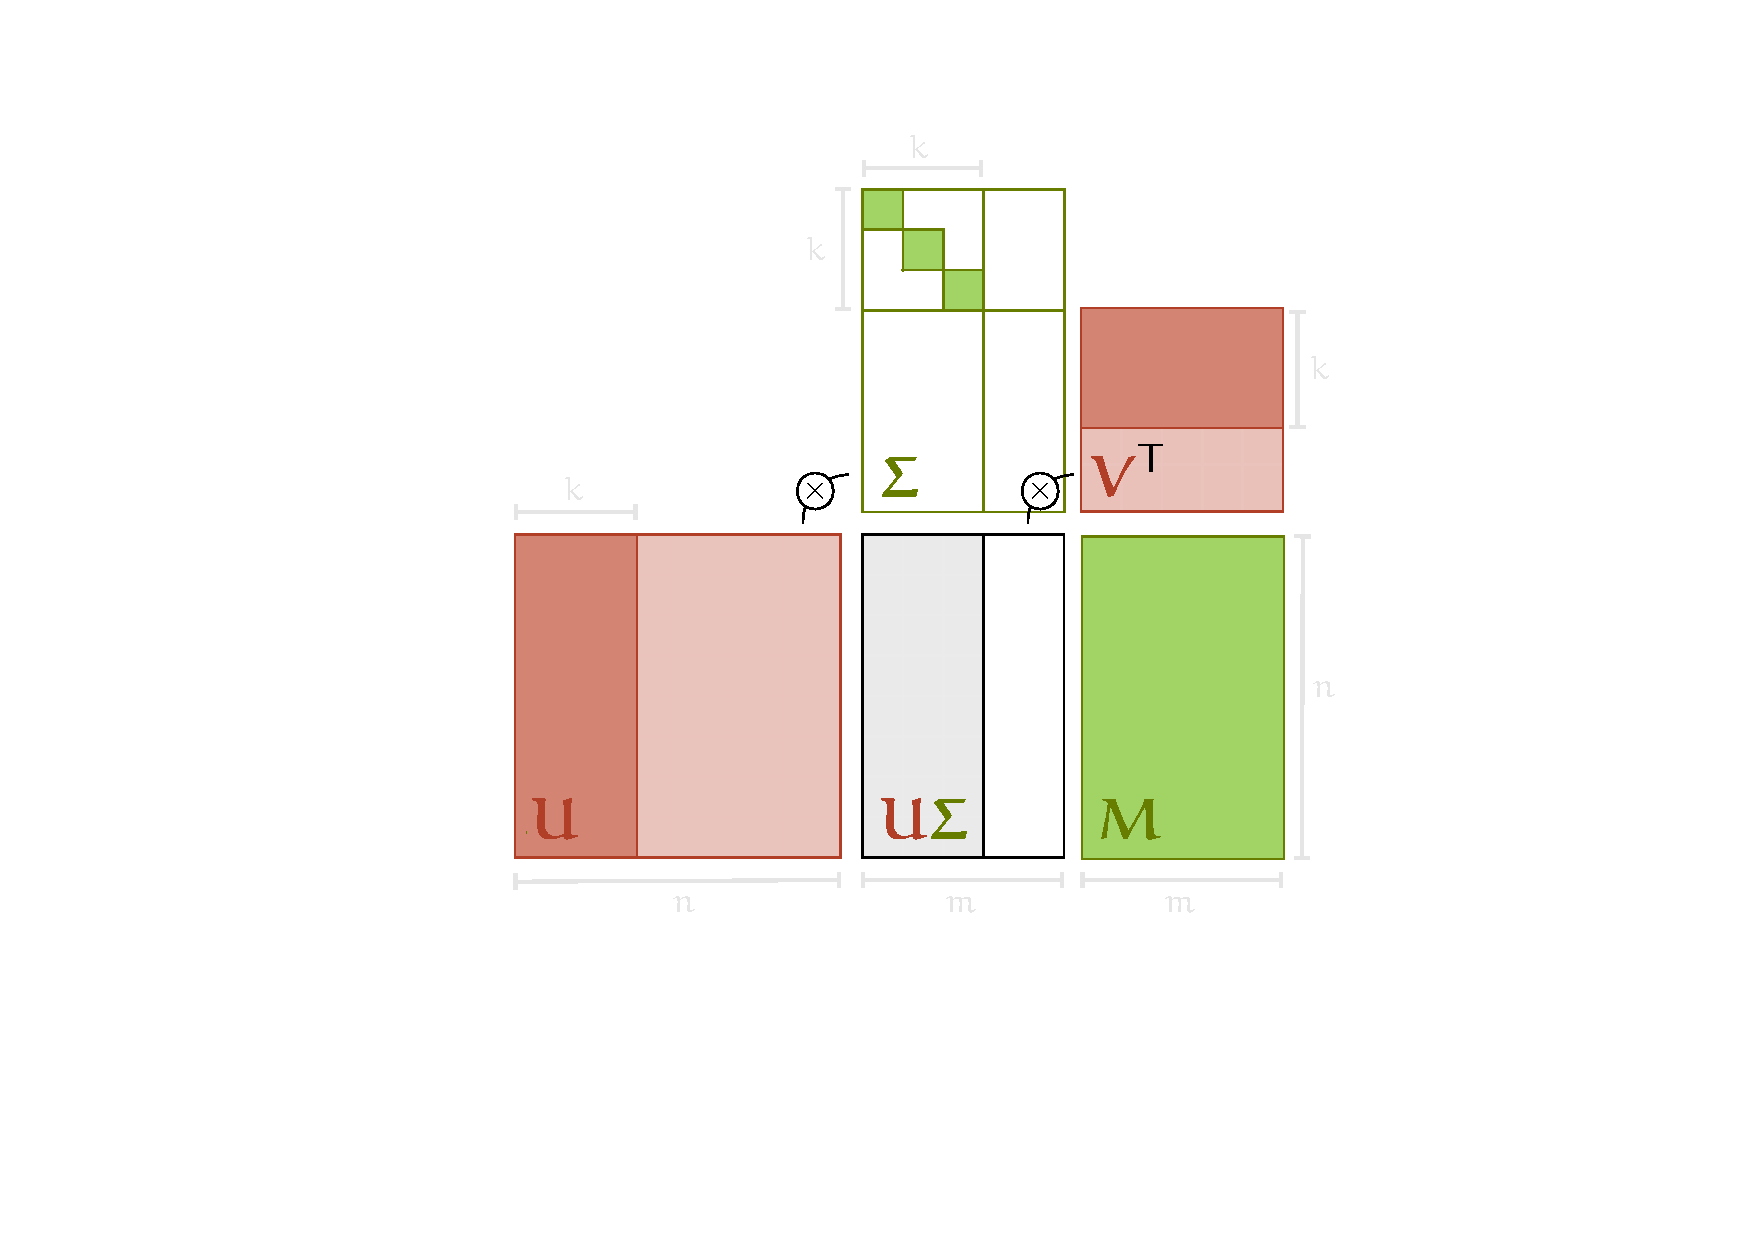
\includegraphics[width=0.7\textwidth]{./images/pca-4/svd-final.pdf}
	}
\end{figure}

%<figure class="narrow centering">
%<img src="/images/pca-4/svd-final.svg" class="three-quarters">
%</figure>

This is called a \textbf{\emph{full} singular value decomposition}. It gives us all singular values, and two  orthonormal bases for \(\mR^n\) and \(\mR^m\).

\index{Full singular value decomposition|textbf}
\index{Singular value decomposition!full}

This is not a very economical way of representing \(\gc{\mbM}\): all these matrices are very big. Let's see if we can trim the fat a little bit.
%
If we look at \(\gc{\Sig}\), we see that we added a lot of zeros, in order to move \(\rc{\mbV}\) over to the right. It seems reasonable, that all these zeros, and their associated basis vectors, aren't actually necessary to represent \(\gc{\mbM}\).

How much do we need? We know that \(\gc{\mbM}\) maps the axes of a sphere in the input space to the axes of an ellipsoid in the output space. Each singular value corresponds to one such mapping from axis to axis. We also know that to get from the equation with only the singular values and vectors to the full SVD, we only added zeros to \(\gc{\Sig}\) and null-space vectors to \(\rc{\mbV}\). It's hard to escape the intuition that we had what we needed already before we extended \(\rc{\mbV}\) and \(\rc{\mbU}\) to be square, and the singular vectors and values by themselves already provided a complete description of \(\gc{\mbM}\).

To prove this, we can walk back the exact steps we took to get to the full SVD, but now with \(\rc{\mbV}\) on the right hand side. First, here is the full SVD, for reference.

\begin{figure}[H]
	\centerline{
		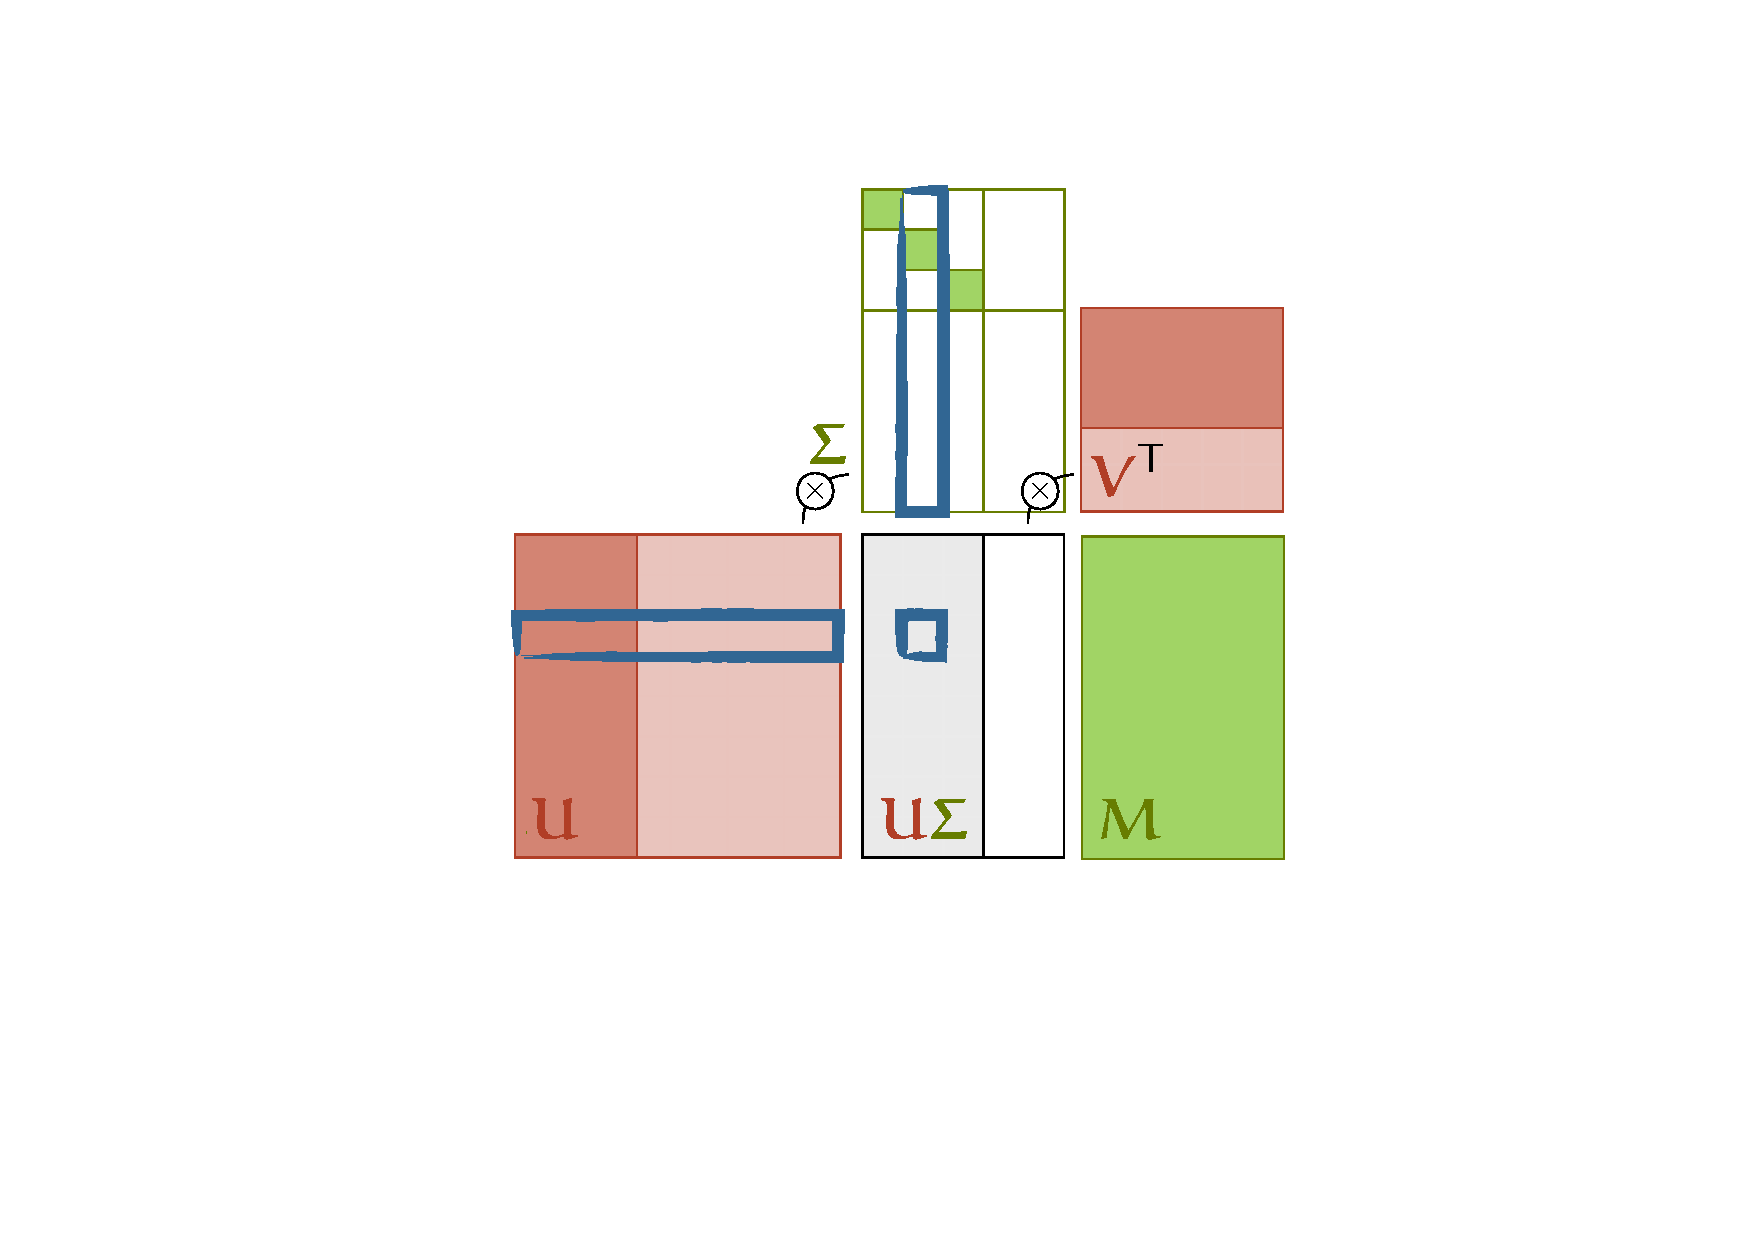
\includegraphics[width=0.7\textwidth]{./images/pca-4/walking-back-step1.pdf}
	}
\end{figure}

%<figure class="narrow centering">
%<img src="/images/pca-4/walking-back-step1.svg" class="three-quarters">
%</figure>

We've highlighted how the elements of \(\rc{\mbU}\gc{\Sig}\) in the middle are computed: each is the dot product of a row of \(\rc{\mbU}\) and a column of \(\gc{\Sig}\). The elements of each are matched up, multiplied and the result is summed together. What we see here, is that the elements of the columns we added to \(\rc{\mbU}\), the ones that don't correspond to a singular value, are always matched up to a zero. Removing them won't change the dot product, and thus won't change the elements of the matrix \(\rc{\mbU}\gc{\Sig}\). This means we can safely remove the columns we added to \(\rc{\mbU}\), and each corresponding row of \(\gc{\Sig}\).

\pagebreak \noindent Here's the result:

\begin{figure}[H]
	\centerline{
		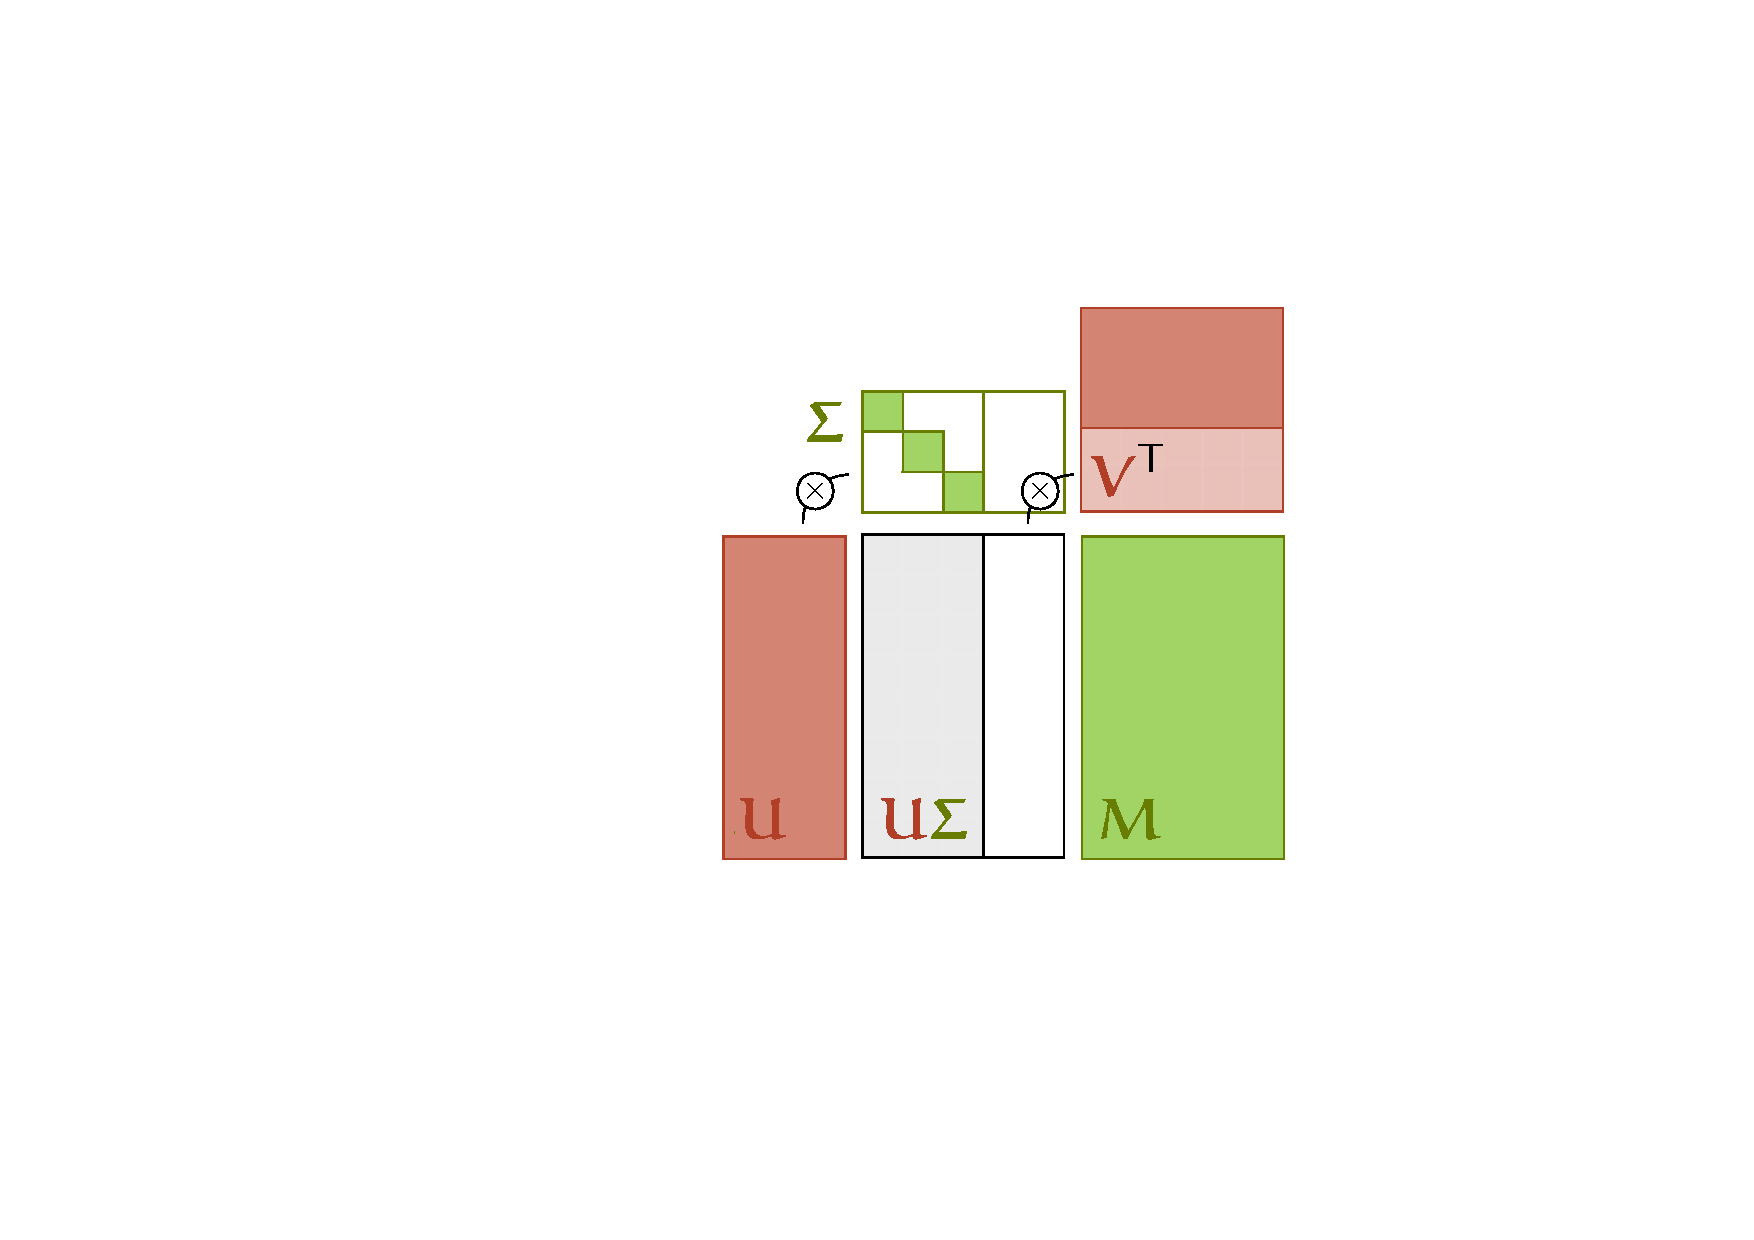
\includegraphics[width=0.7\textwidth]{./images/pca-4/walking-back-step2.pdf}
	}
\end{figure}

%<figure class="narrow centering">
%<img src="/images/pca-4/walking-back-step2.svg" class="three-quarters">
%</figure>

We can use the same logic on the multiplication of \(\rc{\mbU}\gc{\Sig}\) by \(\rc{\mbV}^T\). The added rows of \(\rc{\mbV}^T\) are always matched up to zero columns of \(\rc{\mbU}\gc{\mbZ}\). Removing these will not affect the value of each dot product. To remove the zero columns from \(\rc{\mbU}\gc{\Sig}\), all we need to do is remove the rightmost block of zeros. 

Removing all three, we arrive at a more economical representation of \(\gc{\mbM}\):


\begin{figure}[H]
	\centerline{
		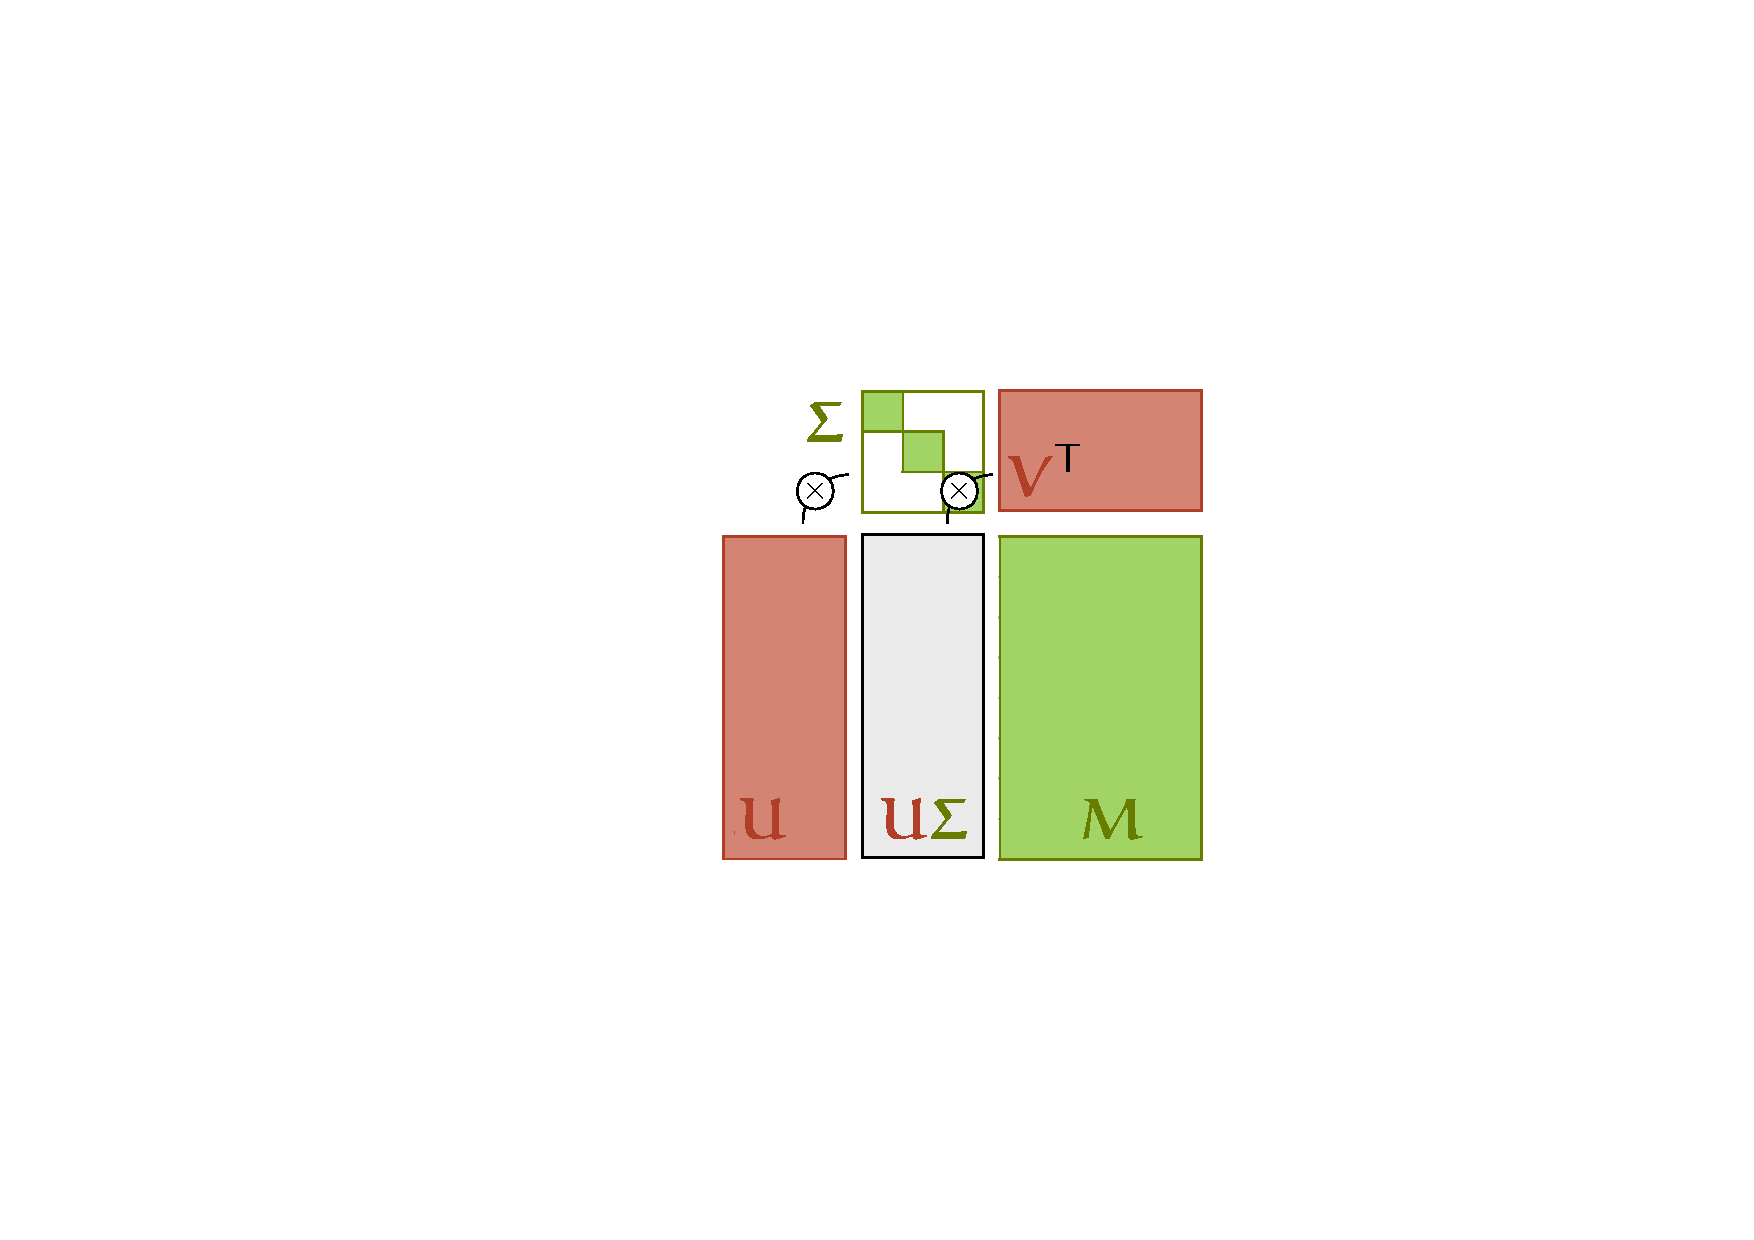
\includegraphics[width=0.7\textwidth]{./images/pca-4/walking-back-step3.pdf}
	}
\end{figure}

%<figure class="narrow centering tight">
%<img src="/images/pca-4/walking-back-step3.svg" class="three-quarters">
%</figure>

It turns out that without extending \(\rc{\mbV}\) and \(\rc{\mbU}\) to full bases, we already had a complete decomposition of \(\gc{\mbM}\), although we had to first make the extension to prove the fact.

We've done a lot of variable reassignments here: first using \(\rc{\mbV}\) to refer to just the singular vectors, then extending it to a square matrix, and then clipping it back again. To make our notation more precise, from now on we'll use \(\rc{\mbU}\) and \(\rc{\mbV}\) for the complete, square, basis matrices and \(\rc{\mbU}_r\) and \(\rc{\mbV}_r\) for the matrices made up of the first \(r\) columns of each.

If we assume that \(\gc{\mbM}\) has \(k\) singular values, we can now write this latest decomposition as:

\[\gc{\mbM} = \rc{\mbU}_k\gc{\Sig}_k{\rc{\mbV}_k}^T
\]

This is called the \textbf{compact SVD}.

\index{Compact singular value decomposition|textbf}\index{Singular value decomposition!compact}


\begin{aside}See the appendix for a more formal proof of the correctness of the compact SVD. 
\end{aside}

Finally, if we're not interested a perfect decomposition, we can extract only the top \(r < k\) singular values and vectors. If we then construct the matrices \(\rc{\mbV}_r\) with the corresponding right singular vectors, \(\rc{\mbU}_r\) with the corresponding left singular vectors and \(\gc{\Sig}_r\) with these singular values along the diagonal, we can still perform the multiplication

\[
\gc{\mbM}_r = \rc{\mbU}_r\gc{\Sig}_r{\rc{\mbV}_r}^T \p
\]

This is called the \textbf{truncated SVD}. It is not a proper decomposition of \(\gc{\mbM}\), since \(\gc{\mbM}_r\) won't be \emph{equal} to \(\gc{\mbM}\), but it will be, in a very precise sense, the closest we can get under these constraints. We'll dig into the details of that later.

\index{Truncated singular value decomposition|textbf}\index{Singular value decomposition!truncated}

\subsection{Principal Component Analysis by SVD}

Before we move on, let's convince ourselves we can actually compute the SVD for a given \(\gc{\mbM}\). The derivation of the SVD we've used above suggests a simple algorithm to decompose a matrix \(\gc{\mbM}\). We can use gradient descent to find the singular vector \(\rc{\mbv}\) for which \(\| \gc{\mbM}\rc{\mbv} \|\) is maximal, subject to the constraint that \(\rc{\mbv}\) is a unit vector. Once gradient descent has converged, we find the next vector in the same way, but with the added constraint that it is orthogonal to all the vectors we've already chosen.

\begin{aside}This is of course, similar to how we computed the PCA in the first chapter. Like in that chapter, we can enforce the constraints by projecting back to an orthogonal unit vector after the gradient update step. 
\end{aside}

If we stop collecting vectors at some arbitrary \(r\), we get the truncated SVD. If we stop when we see the first \(\rc{\mbv}\) for which \(\gc{\mbM}\rc{\mbv} = \mathbf 0\), we get the compact SVD, and finally, if we then also extend \(\rc{\mbV}\) and \(\rc{\mbU}\) to full bases, we get the full SVD.

\index{Computing SVD!by projective gradient descent}

This isn't the most precise or efficient SVD algorithm, and it isn't much better than the algorithm that we already developed for computing PCA in Chapter \ref{chapter:introduction}, but for now it should suffice to convince us that we \emph{can} compute the SVD. We'll first see how exactly to implement PCA on the basis of a given algorithm for the SVD. We'll see some better algorithms in the next chapter.

Let \(\mbX\) be the data matrix for our mean-centered data, and let \(\rc{\mbU}\gc{\Sig}\rc{\mbV}\) be its (full) SVD.

It should be clear from the exposition above that once we have the SVD, there isn't a whole lot left to do.

We know that the principal components are the eigenvectors of \(\kc{\frac{1}{n}}\mbX^T\mbX\). The constant factor \(\kc{\frac{1}{n}}\) affects the eigenvalues, but not the eigenvectors, so we are equivalently looking for the eigenvectors of \(\mbX^T\mbX\). These are the right singular vectors of \(\mbX\), which are the columns of \(\rc{\mbV}\) in our SVD.

So, the principal components follow directly from the singular value decomposition. Let's look at some of the things we may want to do with the principal components in practice, and see how we would achieve that.

\paragraph{Projecting the data to a lower dimension} This is probably the main use case of principal component analysis. Reduce the dimensionality of the data so that we can feed it to some expensive algorithms or visualize it in 2D or 3D. To reduce the data to \(r\) dimensions, we need to project it orthogonally onto the first \(r\) principal components. We achieve this by computing the SVD truncated to \(r\), and computing \(\mbZ = \mbX\rc{\mbV}_r\).

As we can see in the decomposition, this is equal to \(\rc{\mbU}_r\gc{\Sig}_r\). This multiplication is cheaper and more stable to compute, because \(\gc{\Sig}_r\) is a diagonal matrix.

\index{Dimensionality reduction!PCA}
\enlargethispage{1em}

%<!-- The result is that for each instance \(\x\) we get a _latent_ representation \(\z\). -->
\paragraph{Recovering the data} As we saw in Chapter~\ref{chapter:introduction}, we can partly reconstruct the data based on these lower-dimensional representations. Each element \(z_i\) of the latent representation tells us that we should multiply the \(i\)-th principal component by this value, and and sum all these together. 

In matrix terms \(\mbX' = \mbZ{\rc{\mbV}_r}^T = \rc{\mbU}_r\gc{\Sig}_r{\rc{\mbV}_r}^T\).

\index{Reconstruction!PCA}

\paragraph{Whitening} In whitening, discussed in Chapter~\ref{chapter:eigenvectors}, we don't want to reduce the dimensionality of the data, we want to transform it so that it takes the shape of a standard normal distribution (or as close as we can get with a linear transformation). For this, we need a full basis \(\rc{\mbV}\), so we should compute at least the first \(m\) singular vectors, and extend \(\rc {\mbV}\) to be square if necessary. Then, we can compute a complete represention of the data \(\mbZ = \mbX\rc{\mbV}^T = \rc{\mbU}_m\gc{\Sig}_m\).

\index{Whitening!PCA}

This projects the data onto the eigenbasis, but we still need to scale the data along each axis, so that it has unit variance. In 1D, we to this by dividing by the standard deviation, and we characterized the singular values as the analogue of the standard deviation, so it would be intuitive if we should divide by the singular values.

To prove this, remember from Chapter~\ref{chapter:eigenvectors} that the whitening transformation is the inverse of \(\mbx = \bc{\mbA}\mbz + \oc{\mbt}\). That is

\[
\mbz = \bc{\mbA}^{-1}(\mbx - \oc{\mbt}) = \bc{\mbA}^{-1}\mbx - \kc{{\mbA}^{-1}{\mbt} }\p
\]

We'll assume that our data is mean-centered, so \(\oc{\mbt} = {\mathbf 0}\).

We also saw that \(\bc{\mbA}\) should be a square root of the covariance matrix:

\[
\bc{\mbA}\bc{\mbA}^T = \kc{\frac{1}{n}}\mbX^T\mbX
\]

If we expand \(\mbX\) into its SVD, we see that the SVD allows us to compute this square root:

\begin{align*}
\bc{\mbA}\bc{\mbA}^T &= \kc{\frac{1}{n}}\mbX^T\mbX \\
&= \kc{\frac{1}{n}} (\rc{\mbU}\gc{\Sig}\rc{\mbV}^T)^T\rc{\mbU}\gc{\Sig}\rc{\mbV}^T \\
&= \kc{\frac{1}{n}} \rc{\mbV}\gc{\Sig}\rc{\mbU}^T\rc{\mbU}\gc{\Sig}\rc{\mbV}^T \\
&= \kc{\frac{1}{\sqrt{n}}} \rc{\mbV}\gc{\Sig} \kc{\frac{1}{\sqrt{n}}}\gc{\Sig}\rc{\mbV}^T \\
\end{align*}

This means that with \(\bc{\mbA} = \kc{\frac{1}{\sqrt{n}}}\rc{\mbV}\gc{\Sig}\) we have found our square root of the covariance. Not only that, we also have it in a form that is easy to invert:

\begin{align*}
\bc{\mbA}^{-1} &= \left(\kc{\frac{1}{\sqrt{n}}}\rc{\mbV}\gc{\Sig}\right)^{-1} \\
&= \kc{\sqrt{n}}\gc{\Sig}^{-1}\rc{\mbV}^T \\
\end{align*}

where \(\gc{\Sig}^{-1}\) consists simply of \(\gc{\Sig}\), but with the diagonal elements inverted. We can now use \(\bc{\mbA}^{-1}\) to normalize our data.

Note that because we computed an SVD, the inversion, which is normally a very unstable operation, becomes very stable. It isolates the inversion of scalars to the diagonal elements of a matrix, and reduces the rest to transposing an orthogonal matrix.

\begin{aside}This idea, that an SVD is a good way to invert a matrix, runs much deeper, as we shall see when we come to the pseudo-inverse.\end{aside}

\paragraph{Wide data} So far, we've assumed that our data is \emph{tall}. That is, we have many more instances than features. If the reverse is true, as it was for the dataset of faces in Chapter~\ref{chapter:introduction}, we may want to be careful how we compute the SVD. If we have precise control over how many singular vectors we compute, the distinction doesn't matter. Some implementations, however always compute a number corresponding to the width of the input matrix. In this case, with wide data, it may be better to compute the SVD of the transpose, from which we can get the correctly reduced version of the original SVD:

\index{Tall data}\index{Wide data}

\[
\mbX^T = \left(\rc{\mbU}_n\gc{\Sigma}_n\rc{\mbV}_n^T\right)^T = \rc{\mbV}_n\gc{\Sigma}_n\rc{\mbU}_n^T\] 

So that's the SVD: a decomposition that is so similar to PCA, you may be wondering why we separate the two at all? Isn't computing the SVD the same as computing the PCA? The answer is that the SVD is not \emph{just} a way to compute a PCA. It can be used to compute many other things as well.

Next, we'll take a look at some of the most important things the SVD can do for us, beside computing a PCA. Along the way we'll try to build some additional intuition for how the SVD operates.

The first use case will provide an intuition for the number of singular values we can expect in a matrix.

\section{Rank}

\index{Rank}\index{Matrix rank}

Think back to the income dataset from the very first chapter, before we made it more realistic by adding some noise.

\begin{figure}[H]
	\centerline{
		\includesvg[width=0.7\textwidth]{./images/pca/income1.svg}
	}
	\caption*{A plot of monthly salary vs. quarterly income for a small sample of people. Since there is a simple linear relation between these two quantities, the data lies on a straight line.
	}
\end{figure}

%<figure class="narrow centering">
%<img src="/images/pca/income1.svg" >
%<figcaption>A plot of monthly salary vs. quarterly income for a small sample of people. Since there is a simple linear relation between these two quantities, the data lies on a straight line.
%</figcaption>
%</figure>

Even though this data is presented as two-dimensional---with two features---it is really inherently one-dimensional. This is easy to see in the picture, since the data lies on a line. What does this look like in the data matrix \(\mbX\)? Note that each \(x\) value can be derived from the \(y\) value by multiplying it by \(3\). This means that the second column of our data matrix is a \emph{multiple} of the first. For every row \(r\), \(\mbX_{r1} = 3\mbX_{r2}\).

Interestingly, the same holds true in the vertical direction. If we think of each person in the data as a vector, all these vectors point in the same direction. Only their lengths differ. This means that if we fix some arbitrary instance \(i\), desribed by \(\mbx_i\), the \(i\)-th row of \(\mbX\), every other instance (every row in \(\mbX\)) can be described as some scalar \(m\) times \(\mbx_i\).

In some sense, this tells us that the matrix \(\mbX\) is \emph{compressible}. We are given \(300 \cdot 2 = 600\) numbers, but we really only need one vector in \(\mR^{300}\) and a single scalar, or one vector in \(\mR^2\) and \(299\) scalars.

\index{Compressibility}

\begin{figure}[H]
	\centerline{
		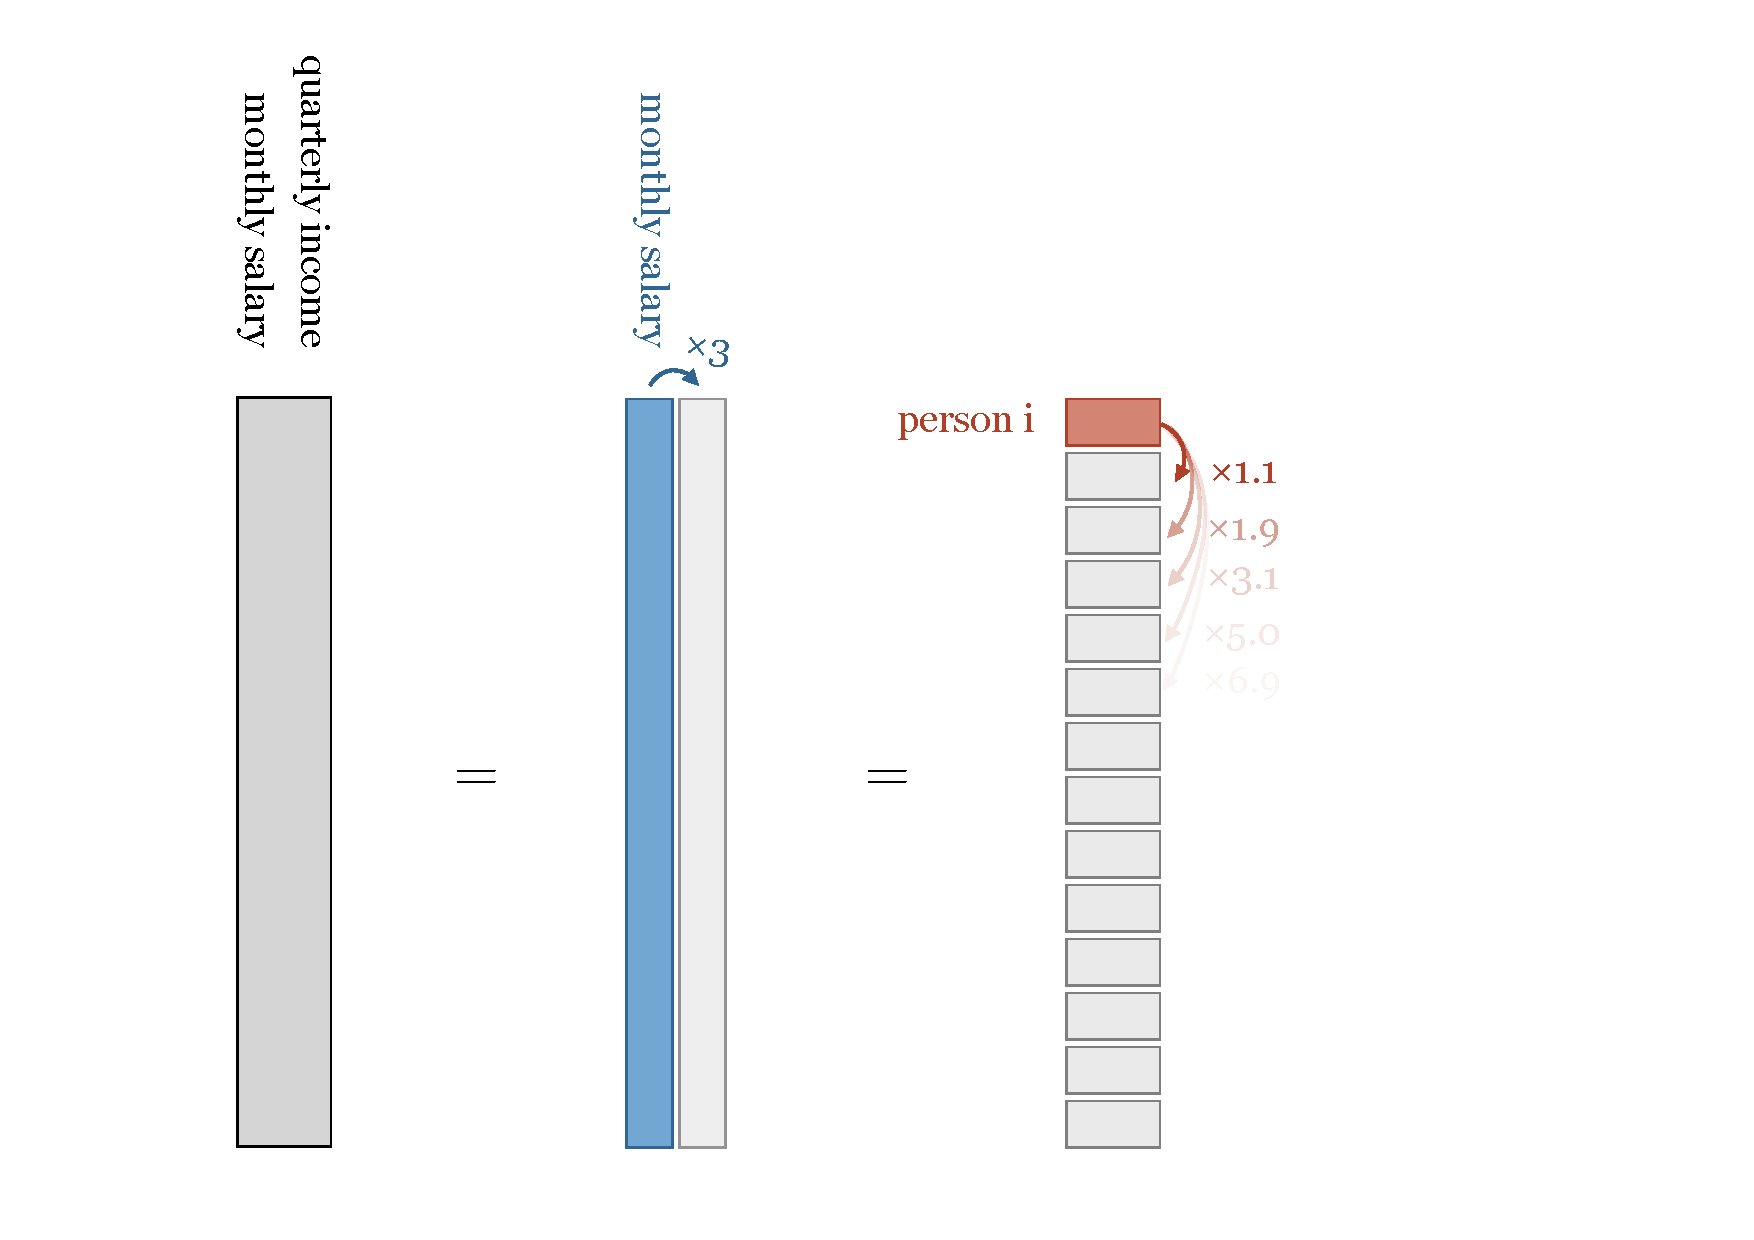
\includegraphics[width=0.7\textwidth]{./images/pca-4/rank-intuition.pdf}
	}
	\caption*{We can represent the data by storing the monthly salary of all subjects and multiplying it by \(\bc{3}\) to get the quarterly income, or we can store one reference person, together with \rc{a multiplier} for every other person in the data.
	}
\end{figure}

%<figure class="narrow centering">
%<img src="/images/pca-4/rank-intuition.svg" class="three-quarters">
%<figcaption>We can represent the data by storing the monthly salary of all subjects and multiplying it by \(\bc{3}\) to get the quarterly income, or we can store one reference person, together with <span class="rc">a multiplier</span> for every other person in the data.
%</figcaption>
%</figure>

How much a matrix can be compressed in this way is indicated by its \textbf{rank}. In this case the horizontal reduction tells us that the matrix has a \emph{column rank} of one---we can represent it by just one of its columns and a bunch of multipliers.

\index{Column rank}\index{Rank!column}

It has \emph{row rank} of one as well---we can also represent it by one of its rows and a bunch of multipliers. We will see in a bit that it is no accident that the row and column rank are the same.

\index{Row rank}\index{Rank!row}

What does it mean to have a rank higher than one? Let's say that a matrix can be \emph{compressed} to \(n\) columns if a subset of \(n\) of its columns is enough to express the rest as a linear combination of these \(n\). For instance, if a matrix has column rank of \(3\), then there are three column vectors \(\mba\), \(\mbb\), and \(\mbc\), so that every other column can be expressed as \(\rc{a}\mba + \rc{b}\mbb + \rc{c}\mbc\) with some numbers \(\rc{a}, \rc{b}, \rc{c}\) unique to that column. The column rank of a matrix is the smallest number of columns that it can be compressed to, and and the row rank is the smallest number of rows that it can be compressed to.

\index{Linear combination}

It's helpful to draw such a compression in as a matrix multiplication. Let's assume we have a large rectangular matrix \(\gc{\mbM}\) with dimensions \(n \times m\) and let's assume that it has column rank \(3\). This means that we can pick three of its columns \(\mba\), \(\mbb\) and \(\mbc\) and represent all other columns by a set of just three numbers \(a\), \(b\) and \(c\).

Before we draw the diagram, note that \(\mba\), \(\mbb\) and \(\mbc\) don't actually \emph{have} to be columns of \(\gc{\mbM}\). We could, for instance, scale them to unit vectors, and we could still represent all columns of \(\gc{\mbM}\) as linear combinations. The key point is that we can express all column vectors of \(\gc{\mbM}\) in some \emph{basis} of three vectors. They are all points in some 3D subspace of \(\mR^n\).

\index{Basis}
\enlargethispage{4em}

Now, to our diagram. Put the three basis vectors \(\mba\), \(\mbb\) and \(\mbc\) side by side in a matrix \(\bc{\mbB}\) of \(n \times 3\). For a given column of \(\gc{\mbM}\), we can work out what \(\rc{a}\), \(\rc{b}\) and \(\rc{c}\) should be and put these together in a column vector \(\rc{\mbd}\). Multiplying \(\bc{\mbB}\rc{\mbd}\) gives us the linear combination \(\rc{a}\mba + \rc{b}\mbb + \rc{c}\mbc\), and thus reconstructs our column vector of \(\gc{\mbM}\). If we work out all the vectors \(\rc{\mbd}\) for all columns of \(\gc{\mbM}\) and concatenate them as the columns of a big \(3 \times m\) matrix \(\rc{\mbD}\), then multiplying \(\bc{\mbB}\rc{\mbD}\) reconstructs all columns of \(\gc{\mbM}\). Or, put simply, \(\gc{\mbM} = \bc{\mbB}\rc{\mbD}\).

\begin{figure}[H]
	\centerline{
		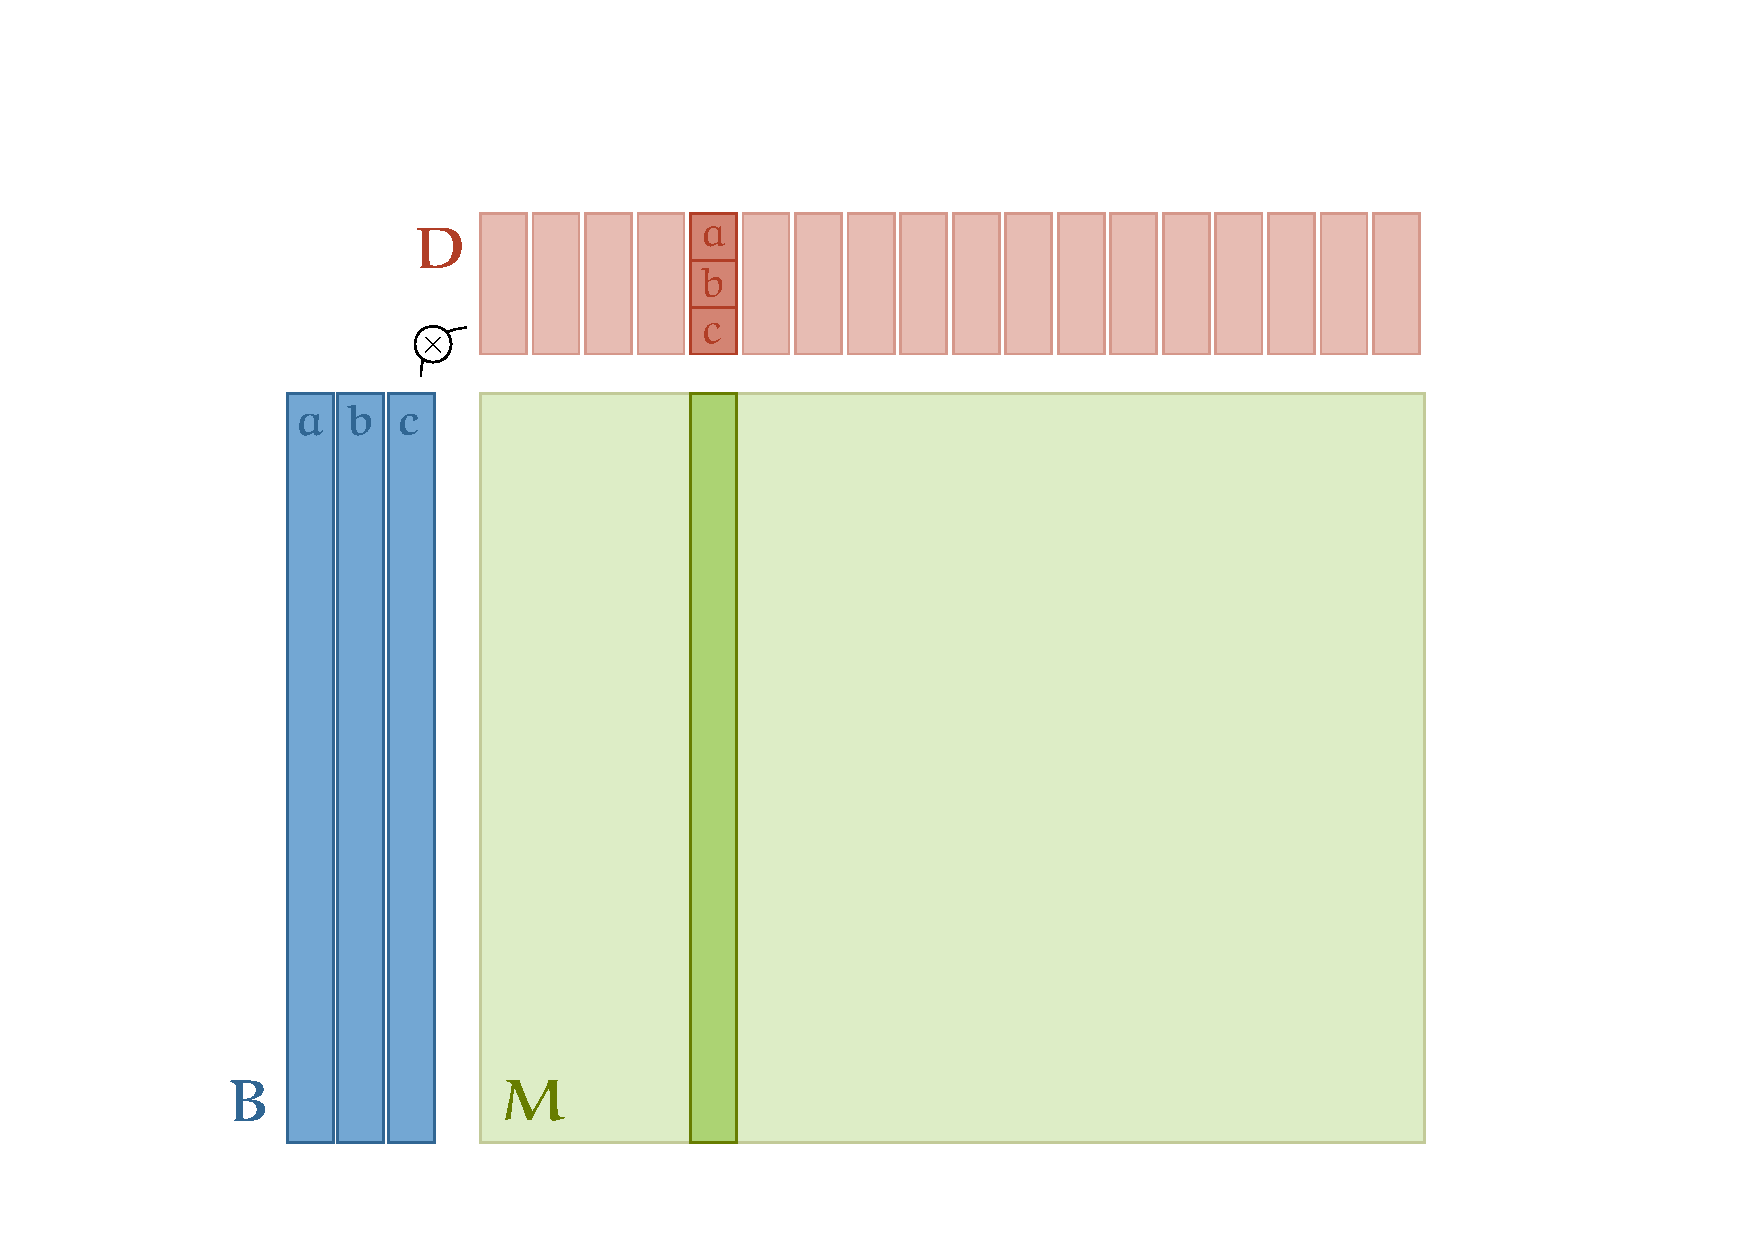
\includegraphics[width=0.59\textwidth]{./images/pca-4/rank1.pdf}
	}
	\caption*{A matrix \(\gc{\mbM}\) with column rank \(3\) can be written as the multiplication of an \(\bc{n \times 3}\) matrix and a \(\rc{3 \times m}\) matrix.
	}
\end{figure}

%<figure class="narrow centering">
%<img src="/images/pca-4/rank1.svg" class="three-quarters">
%<figcaption>A matrix \(\gc{\M}\) with column rank \(3\) can be written as the multiplication of an \(\bc{n \times 3}\) matrix and a \(\rc{3 \times m}\) matrix.
%</figcaption>
%</figure>

This is called a \textbf{rank decomposition} of \(\gc{\mbM}\).

\index{Rank decomposition}\index{Decomposition!rank}

Looking at this diagram, we can almost directly deduce one of the more magical facts about ranks: \textbf{that the column rank is equal to the row rank}.

\index{Rank!equality of column - and row -|(}

Imagine if we were to follow the same recipe for the row rank. We don't know the row rank, so let's call it \(k\). If the row rank is \(k\), there will be \(k\) rows that can serve as a basis for all rows. We concatenate them into a \(k \times m\) matrix \(\bc{\mbB}'\) and work out the row vectors \(\rc{\mbd}'\) for each row of \(\gc{\mbM}\). Concatenating these into a matrix \(\rc{\mbD}'\) of \(n \times k\), we get \(\rc{\mbD}'\bc{\mbB}' = \gc{\mbM}\). In other words, we get exactly the same diagram, but with the roles reversed.

\vspace{-0.8em}
\begin{figure}[H]
	\centerline{
		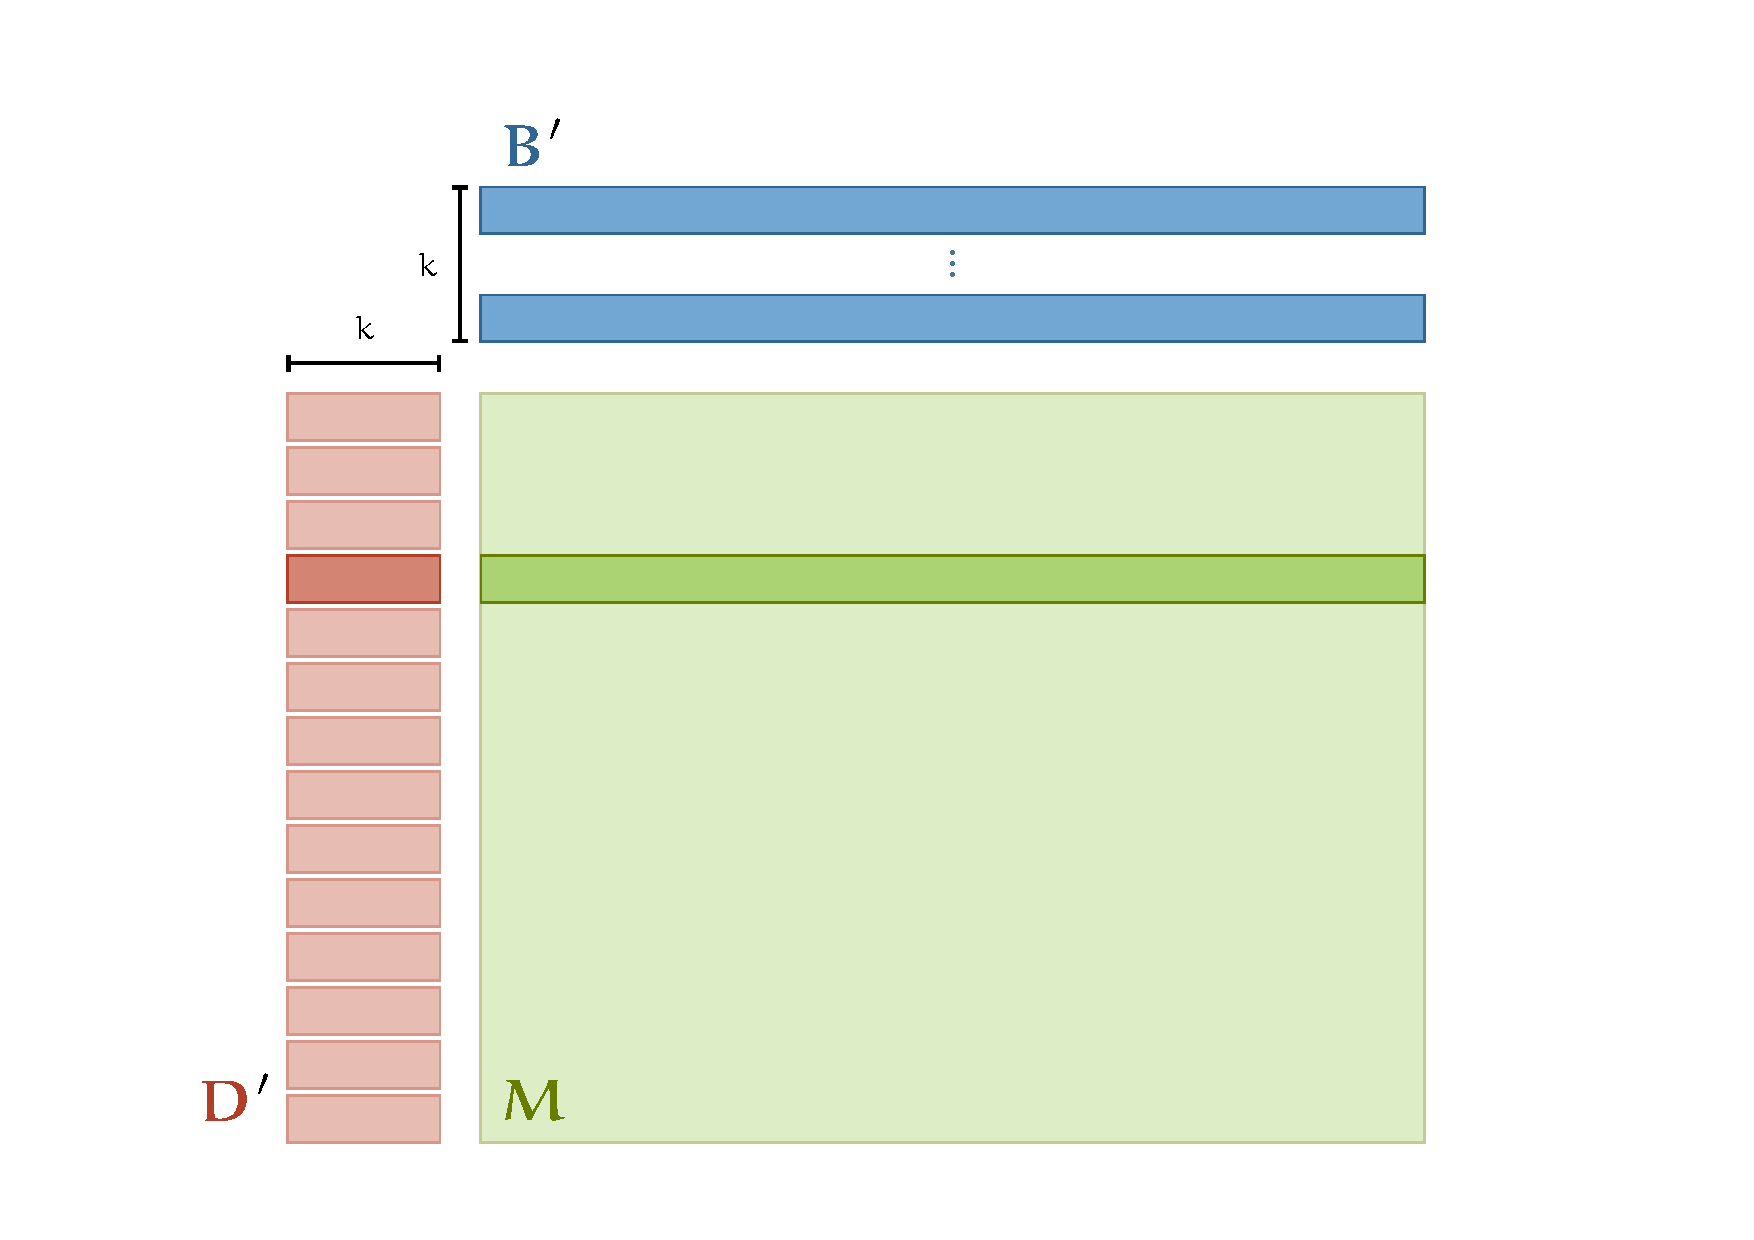
\includegraphics[width=0.62\textwidth]{./images/pca-4/rank2.pdf}
	}
\end{figure}

%<figure class="narrow centering">
%<img src="/images/pca-4/rank2.svg" class="three-quarters">
%</figure>

This means that in the second diagram, we can also interpret \(\rc{\mbD}'\) as representing \(k\) column vectors and \(\bc{\mbB}'\) as representing the scalars required to reconstruct the columns of \(\gc{\mbM}\). And from this we can deduce directly what \(k\) should be. Since \(3\) is the column rank of \(\gc{\mbM}\), \(k\) can't be less than \(3\) or we would have found a representation of \(\gc{\mbM}\) in fewer columns (and the rank is the lowest number of columns possible). It also can't be more than \(3\), because then we could go the other way around: start with the second diagram, interpret it as a row rank diagram, and we'd find a representation with fewer rows than \(k\), even though \(k\) is the row rank. So \(k\) must be \(3\).

This argument shows us that the column and the row rank of any matrix \emph{must} be equal. We can drop the qualifier, and just refer to the matrix's \textbf{rank}. We can also conclude that the maximum possible value of the rank is \(\text{min}(n, m)\): the column rank cannot exceed the number of columns, and the row rank cannot exceed the number of rows, so the minimum of these two must be the matrix rank.

A matrix with rank equal to \(\text{min}(m, n)\) is called \emph{full rank}. A matrix that isn't full rank is called \emph{rank deficient}.

\index{Rank!equality of column - and row -|)}

\index{Full rank matrix}\index{Rank deficient}

The rank is a very fundamental property of matrices with many interpretations in many contexts. Here are three examples, the last of which will bring us back to the singular value decomposition.

\paragraph{Dimension of the image of \(\gc{\mbM}\)} In Chapter~\ref{chapter:spectral-theorem}, to explain the determinant, we modeled the operation of a square matrix as a mapping from a unit cube to a polyhedron. We can extend this intuition to rectangular matrices as well. Take an \(n \times m\) matrix \(\gc{\mbM}\). The input space of this matrix is spanned by \(m\) unit vectors pointing along the axes of \(\mR^m\). If we imagine these as \(m\) sides defining a unit cube, then we can ask how this cube is transformed by \(\gc{\mbM}\) into a parallelotope in \(\mR^n\).

The input vectors are one-hot, so multiplying one by \(\gc{\mbM}\) just picks out one of the columns of \(\gc{\mbM}\). Thus, we are creating the parallelotope spanned by the columns of \(\gc{\mbM}\). If all of these point in different directions, the parallelotope is of dimension \(m\). If we only get \(r < m\) unique directions, we get an \(r\)-dimensional shape.

\pagebreak \noindent We also get a shape of less than \(m\) dimensions if one or more of the vectors lies in a plane spanned by two of the others, or more generally in an subspace spanned by some of the others. In short, if one of the vectors is a linear combination of the rest.

The rank of \(\gc{\mbM}\) tells us the dimension of the \emph{image}: the shape we get after operating on a shape of dimension \(m\). Since column and row rank are equal, we now know that this is also the dimension of an image of \(\gc{\mbM}^T\). In the image below, we look at the image of the unit cube under a matrix. Since the matrix has rank two, the resulting figure is two-dimensional.

\index{Image!of a matrix}

\begin{figure}[H]
	\centerline{
		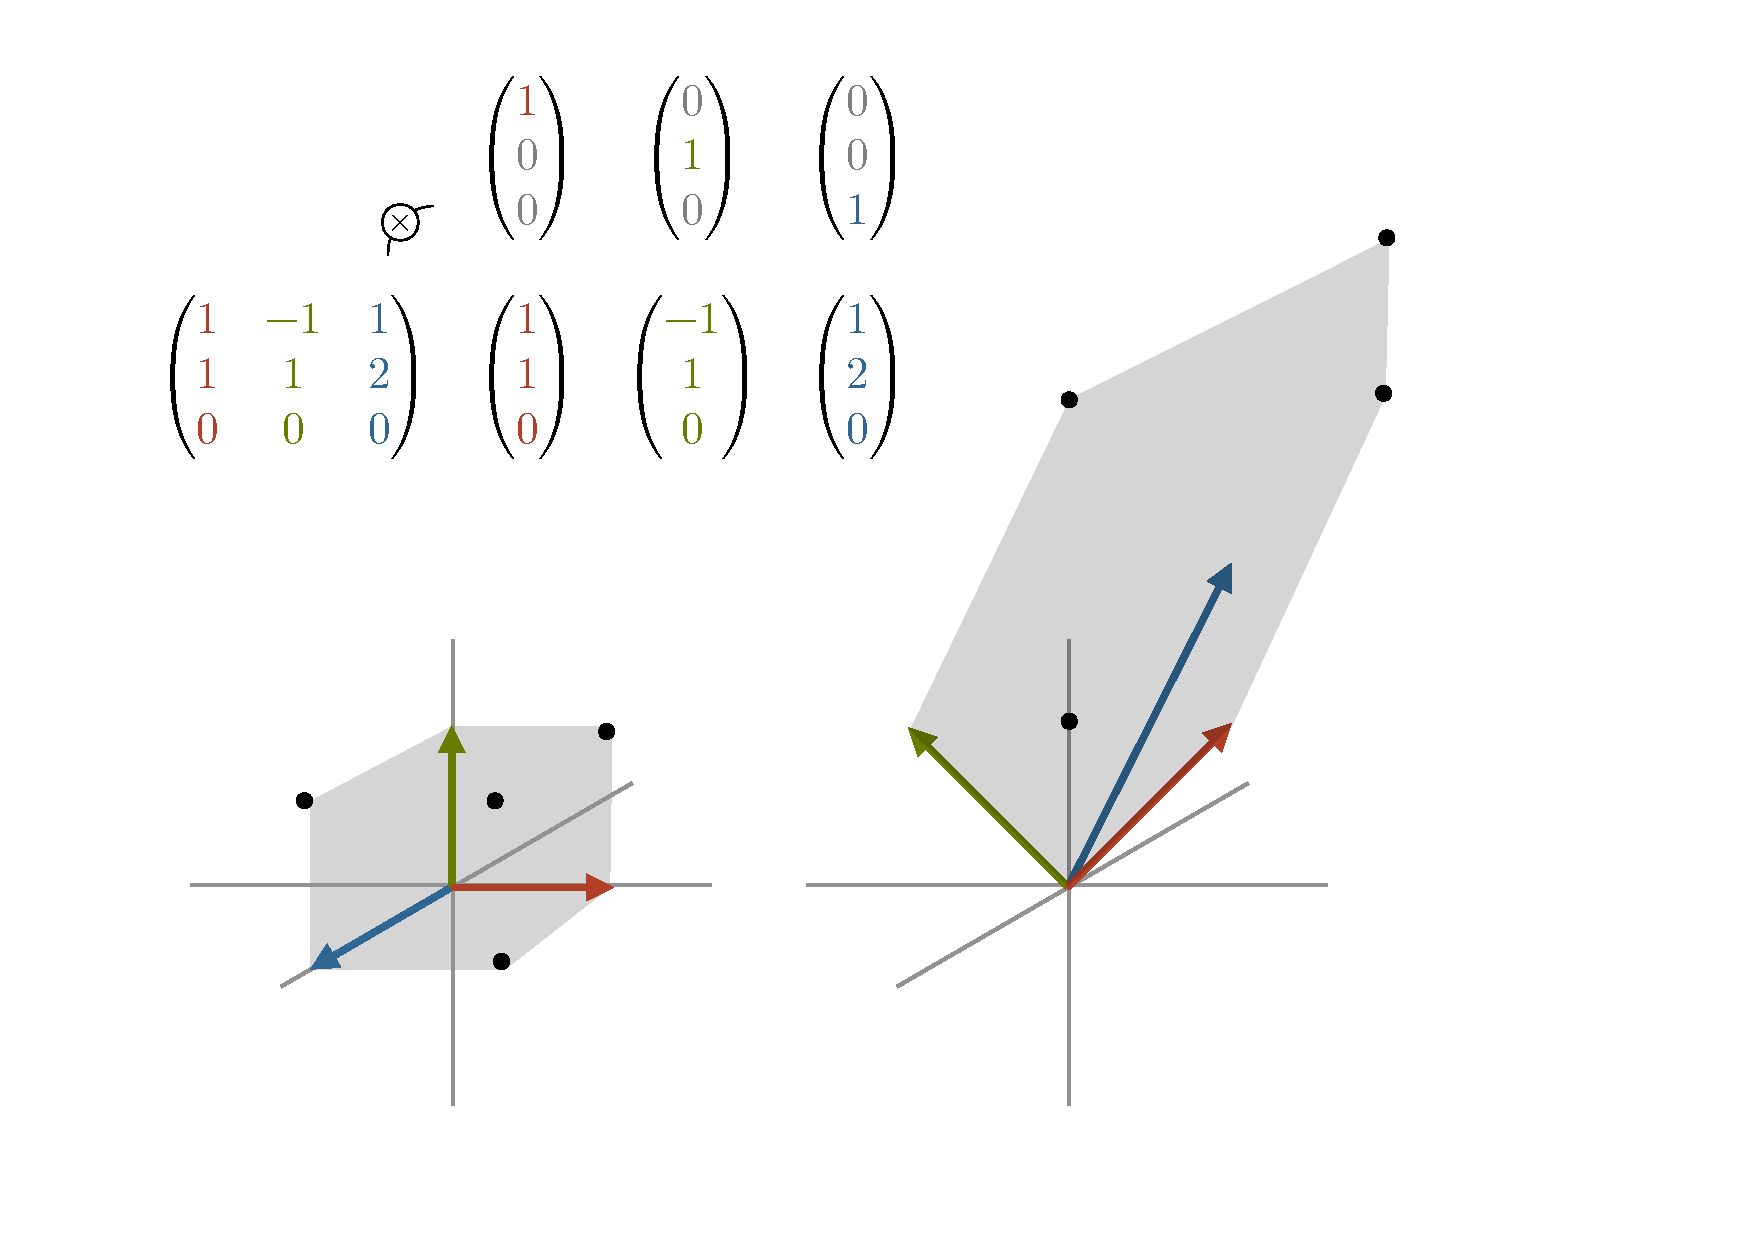
\includegraphics[width=0.85\textwidth]{./images/pca-4/image-dim.pdf}
	}
	\caption*{The matrix above maps the three standard basis vectors to three different points in space that correspond to the columns of the matrix. The matrix has low rank because we can express \bc{one column} as the sum of the the \rc{other} \gc{two}. This means that the unit cube is flattened into a two-dimensional sheet containing all three vectors.}
\end{figure}

%<figure class="narrow centering">
%<img src="/images/pca-4/image-dim.svg" class="three-quarters">
%<figcaption>The matrix above maps the three standard basis vectors to three different points in space that correspond to the columns of the matrix. The matrix has low rank because we can express one column as a linear combination of the other two. This means that the unit cube is flattened into a two-dimensional sheet containing all three vectors.
%</figcaption>
%</figure>

\paragraph{Invertibility and determinants} A square matrix \(\bc{\mbA}\) with dimensions \(n \times n\) can be invertible. That means that given \(\mby\), there is always only one \(\mbx\) such that \(\mby = \bc{\mbA}\mbx\). We've already seen that the determinant tells us when a matrix is invertible: if the image of the matrix has volume \(0\), then the matrix is not invertible. Note that we are talking about \(n\)-volume here. If the matrix is \(3 \times 3\) and the image of the unit cube is 2 dimensional, then it has a nonzero area but zero volume. In general if the image of an \(n \times n\) matrix has nonzero \(n\)-volume, the determinant of \(\bc{\mbA}\) is zero.

\index{Invertible matrix!rank of}\index{Singular matrix!rank of}

Any shape of dimension less than \(n\) has zero \(n\)-volume: a square has zero volume, and a line has zero area. This means that if the rank tells us that the image of a \(\bc{\mbA}\) has dimension less than \(n\), \(\bc{\mbA}\) must have determinant \(0\) and must therefore be non-invertible.

The reverse direction also works. If \(\bc{\mbA}\) is full-rank, the image, however small, is \(n\)-dimensional, and must have a nonzero \(n\)-volume. If we look at the image of the unit cube, we see that the images of the standard basis vectors \emph{must} point in different directions if \(\bc{\mbA}\) is full rank, and the resulting parallellotope must have nonzero volume.

This provides one way to check for matrix singularity: if any of the columns is a linear combination of the rest, your matrix must be rank deficient, and therefore non-invertible, and have determinant \(0\). If there is no such column, the matrix is full rank, invertible and has nonzero determinant.

\paragraph{Number of singular values} Here, we come back to the topic at hand. We've defined what singular values are, and how to enumerate them one by one. We've seen that this enumeration stops at some point (when \(\| \gc{\mbM}\rc{\mbv} \| = 0\)), but we haven't talked about \emph{when} we can expect it to stop. How many singular values should we expect a given matrix to have?

\index{Rank!and singular values}

You can probably guess the answer, so let's start there and work backwards: \emph{the number of non-zero singular values a matrix has, is equal to its rank}.

How do we show this? We discussed above that the rank is the dimension of the image of a matrix. That means that if we start with all unit vectors in \(\mR^m\), a sphere of dimension \(m\), and look at the image of this set under \(\gc{\mbM}\), we will see a \(k\)-dimensional ellipsoid. This means that the process that enumerates the singular vectors can spit out \(k\) mutually orthogonal vectors. After that, every vector \(\rc{\mbv}\) that is orthogonal to the ones already produced must have \(\gc{\mbM}\rc{\mbv} = \mathbf 0\).

\subsection{Computing rank}

\index{Rank!computing|(}

So, that's rank. A fundamental, and very useful property of matrices. Now, given a matrix \(\gc{\mbM}\), how do we \emph{compute} its rank? There are many algorithms: QR decomposition, row reductions, etc. The problem with all of these, is that when we encounter a matrix in the wild, there is often a little bit of noise. Either the matrix contains measurements, which are always subject to noise, or it's the result of some numeric computation, in which case floating point errors probably add a little bit of imprecision.

\index{QR decomposition}

Any small amount of noise means that, with overwhelming probability, no column vectors will lie in \emph{exactly} the subspace spanned by the others. The noise will always push it a tiny bit out of the subspace. This will technically make the matrix full rank, but what we are actually interested in, is what rank the matrix would have if we could remove the noise.

\enlargethispage{3em}
\begin{figure}[H]
	\centerline{
		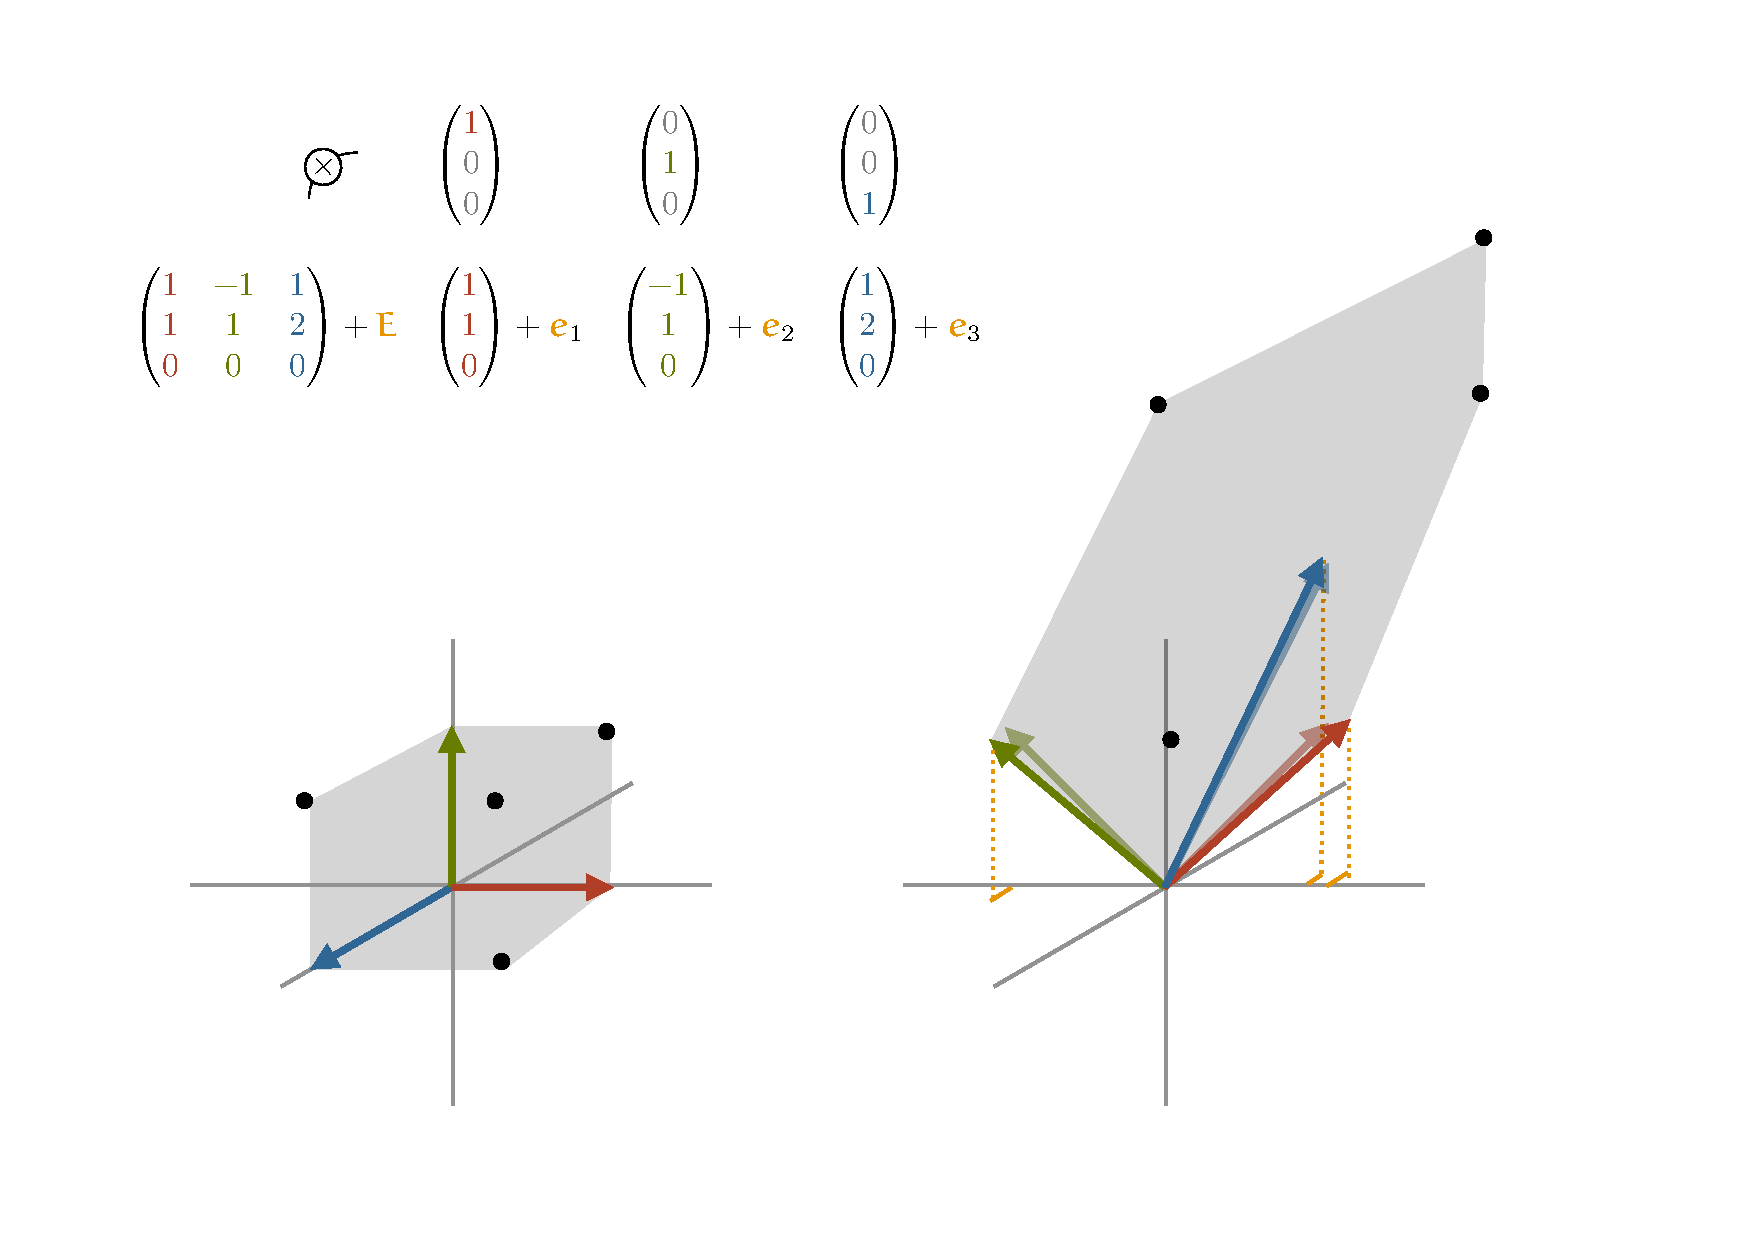
\includegraphics[width=.85\textwidth]{./images/pca-4/low-rank-noise.pdf}
	}
	\caption*{The low-rank matrix we used above, but now with a noise matrix \(\oc{\mbE}\) added to it, containing random values of small magnitude. The result is that each of the columns  is nudged a little in a random direction, pushing it out of the \(xy\)-plane. The image of the unit cube is now no longer a 2D sheet, but a very flat 3D shape.
	}
\end{figure}

%<figure class="narrow centering">
%<img src="/images/pca-4/low-rank-noise.svg" class="three-quarters">
%<figcaption>The low rank matrix we used above, but now with a noise matrix \(\oc{\E}\) added to it containing random values of small magnitude. The result is that each of the columns  is nudged a little in a random direction, pushing it out of the \(xy\)-plane. The image of the unit cube is now no longer a 2D sheet, but a very flat 3D shape.
%</figcaption>
%</figure>

This is why the SVD is the preferred way of computing the rank of a matrix. If  have a column vector that lies almost but not quite in the subspace spanned by the others, the result is \emph{a very small singular value}.

To see why, imagine a rank 1 matrix with dimensions \(3 \times 3\). This matrix would have all column vectors pointing in the same direction, and the image of the unit sphere would be a line segment. As a result, we get one singular value.

If we apply a tiny bit of noise to one of the columns, one of the vectors in the image won't quite point in the same direction as the others. As a result, we get an ellipse that looks a lot like a line segment: very thin in one direction. The image has 2 axes, so we get two singular vectors: one very similar to what we had before, for the main axis of the ellipse, and one very tiny one orthogonal to it, representing the extra dimension created by the noise.

\begin{figure}[H]
	\centerline{
		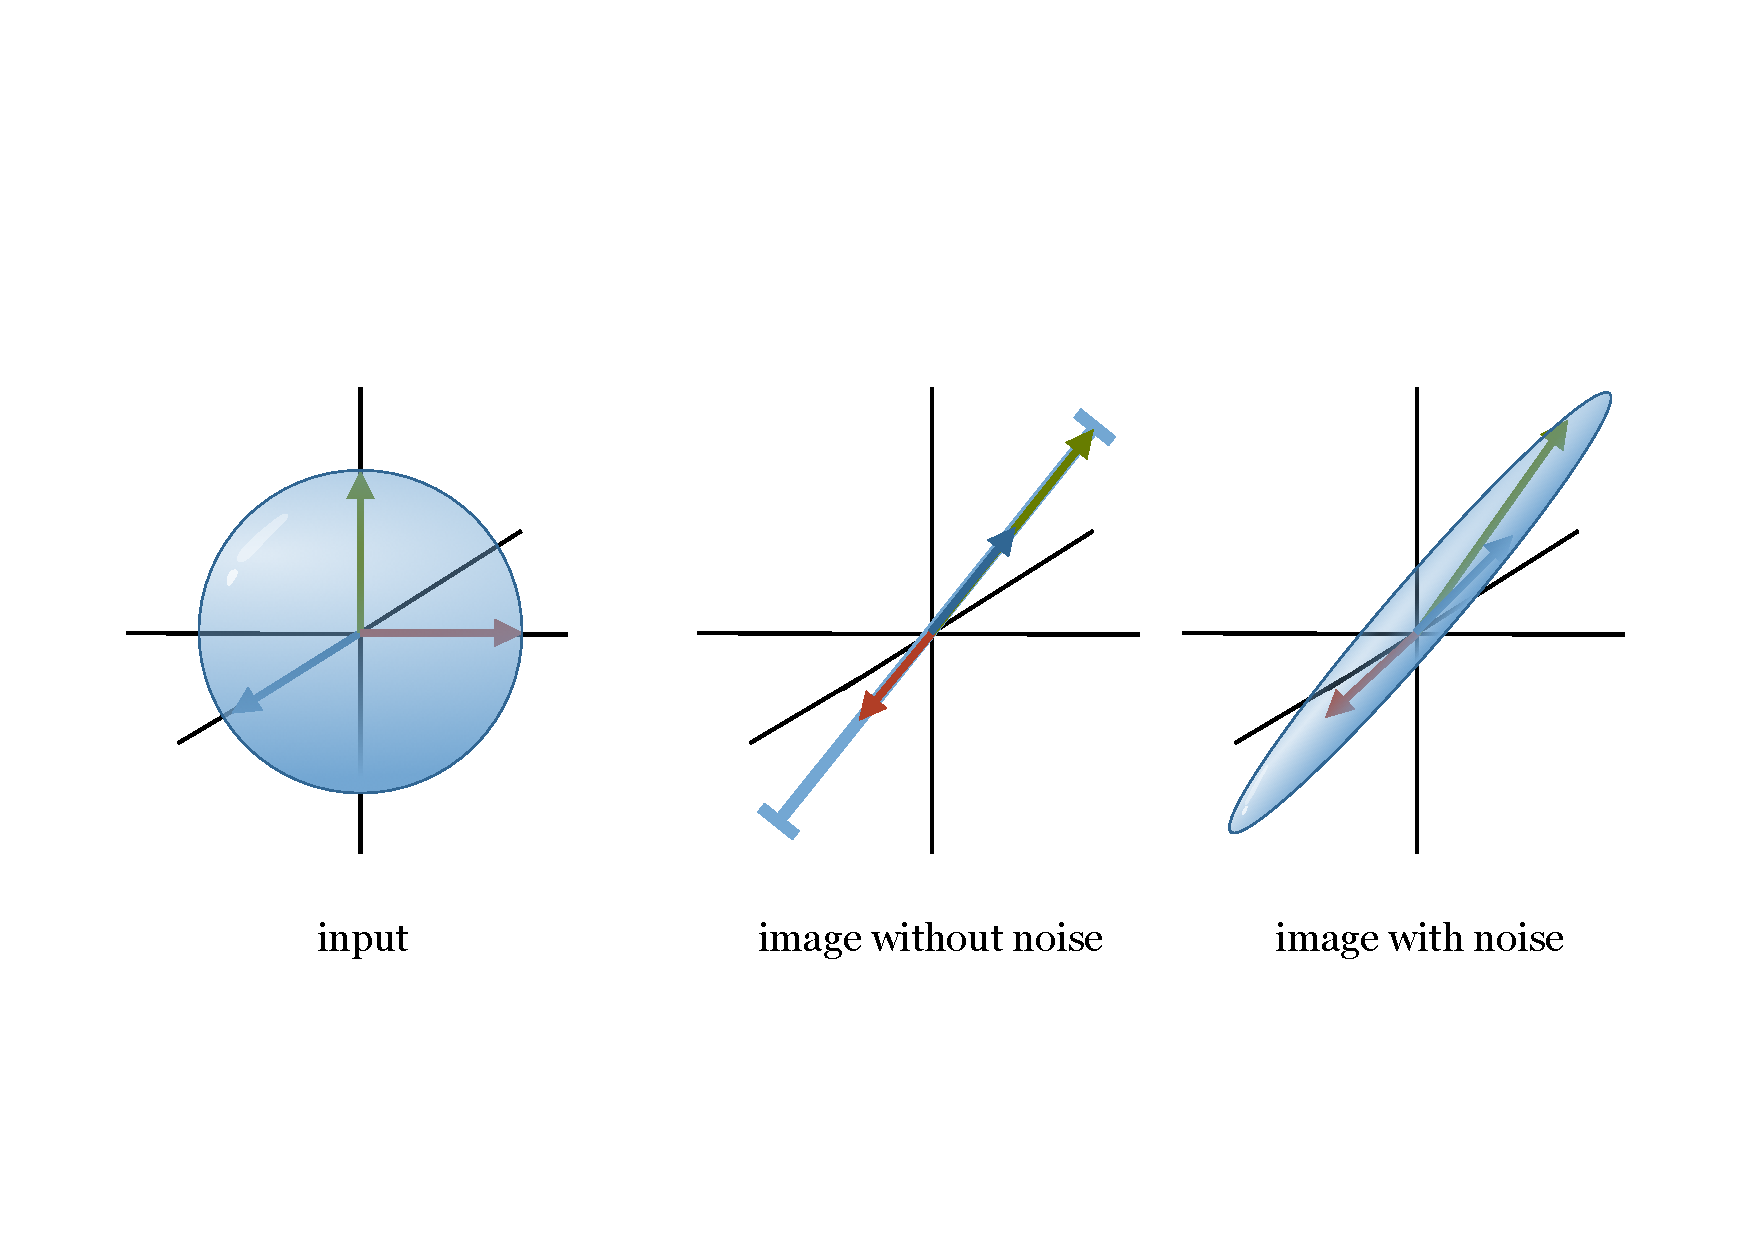
\includegraphics[width=1\textwidth]{./images/pca-4/low-rank-sphere.pdf}
	}
	\caption*{For a rank-1 matrix, the image of the unit sphere is a line segment. If a little noise is added, the image becomes an elongated ellipsoid. Its major axis has large magnitude, corresponding to the original singular value and vector. The other two are very small: these correspond to the singular values introduced by the noise.
	}
\end{figure}

%<figure class="narrow centering tight">
%<img src="/images/pca-4/low-rank-sphere.svg">
%<figcaption>For a rank-1 matrix, the image of the unit sphere is a line segment. If a little noise is added, the image becomes an elongated ellipsoid. Its major axis has large magnitude, corresponding to the original singular value and vector. The other two are very small: these correspond to the singular values introduced by the noise.
%</figcaption>
%</figure>

If the noise is small, then the singular values created by the noise are of an entirely different magnitude to the original singular values. This is why the SVD helps us to compute the rank in the presence of noise: we simply set a threshold to some low number like \(10^{-7}\), and treat any singular value below the threshold as zero. The number of singular values remaining is the rank of our matrix \emph{if we ignore the noise}.

\index{Rank!computing|)}

What if we were to remove the corresponding singular \emph{vectors} as well? If \(r\) is the rank we've established with the method described above, this means performing an \(r\)-truncated SVD. Multiplying the matrices \(\rc{\mbU}_r\), \(\gc{\Sig}_r\), \(\rc{\mbV}_r\) back together gives us a matrix \(\gc{\mbM}'\) which approximates \(\gc{\mbM}\), but removes the singular vectors corresponding to the noise. Can we treat this as a denoised version of our matrix? If so, what can we say about the remainder?

\index{Matrix denoising}

We can answer that question very precisely, but to do so, we'll first look at how the SVD can help us solve equations.

\section{The pseudo-inverse}

\index{Pseudo-inverse|textbf}

A very common use of the singular value decomposition is to solve systems of linear equations. To put that in a familiar context, let's return again to the example that we started with in Chapter~\ref{chapter:introduction}: the salary dataset. This time, we'll look at the more realistic version.

\begin{figure}[H]
	\centerline{
		\includesvg[width=0.9\textwidth]{./images/pca/income2.svg}
	}
\end{figure}

%<figure class="narrow">
%<img src="/images/pca/income2.svg">
%</figure>

When I first showed this picture, I tried to steer you away from seeing this as a linear regression problem, where the task is to predict the variable on the vertical axis from the one on the horizontal. PCA, after all, is an \emph{unsupervised} method: no feature in our data is marked as the target to be predicted. Instead, we want a compressed representation from which we can ``predict'' all of them as well as possible.

\pagebreak \noindent Let's forget about PCA for the moment, and let's return to the supervised setting. If we do want to predict one feature given the others, how does the SVD help us do this, and how does the solution to this problem relate to the solution to the PCA problem?

We'll stick with linear regression. This means we want to draw a line through these points that provides a prediction for the variable on the vertical axis. We want to choose this line so that the squares of the vertical distance to the data are minimized.

\index{Linear regression}

Here's a comparison to the definition of the first principal component. For the linear regression, we minimize the squares of the vertical distance, while for the principal component, we minimize the squares of the distances across both dimensions.

\begin{figure}[H]
	\centerline{
		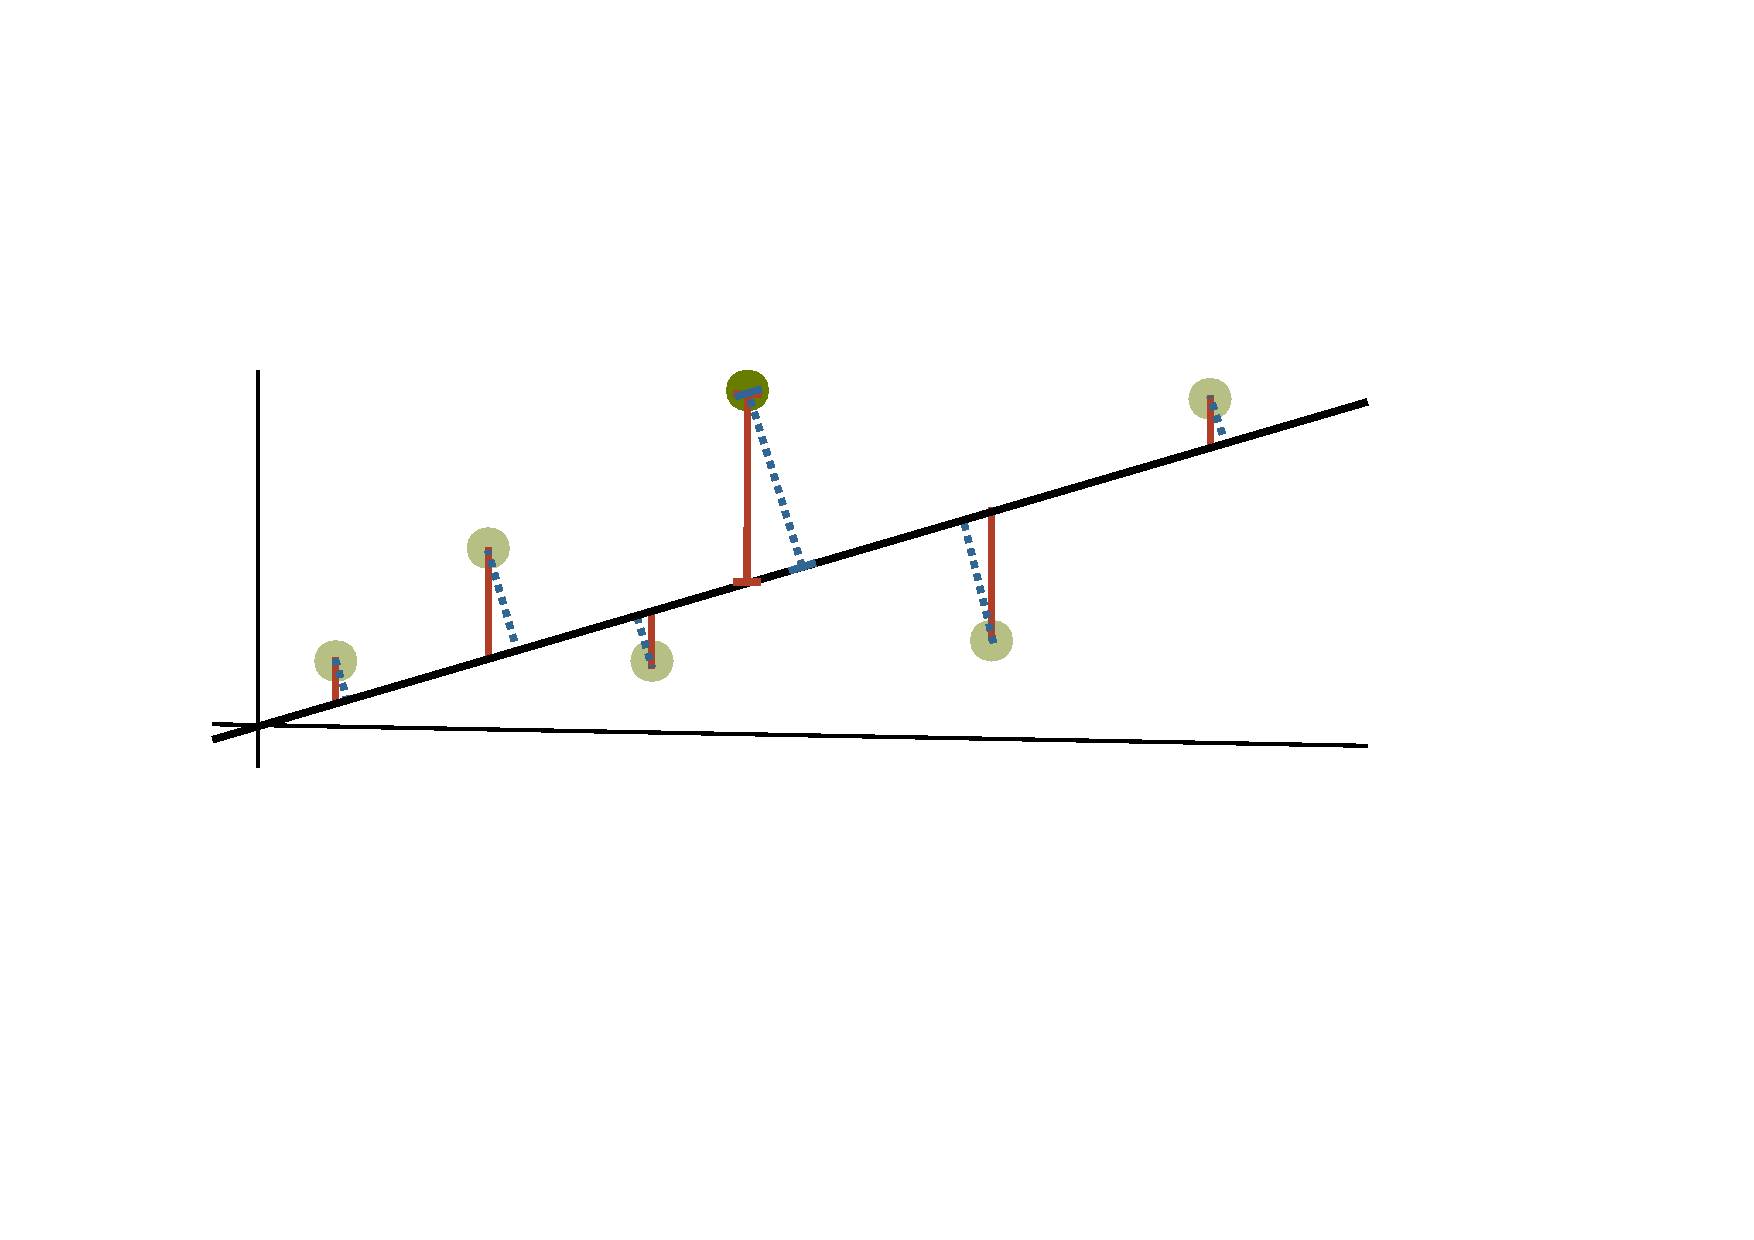
\includegraphics[width=0.8\textwidth]{./images/pca-4/pca-vs-reg.pdf}
	}
	\caption*{In PCA, the objective is to choose the black line to minimize the squared \bc{distances between the data and the line}. In linear regression, we are minimizing only the squares of the \rc{the vertical distances}.}
\end{figure}

%<figure class="narrow">
%<img src="/images/pca-4/pca-vs-reg.svg">
%<figcaption>In PCA, the objective is to choose the black line to minimize the squared <span class="bc">distances between the data and the line</span>. In linear regression, we are minimizing only the squares of the <span class="rc">the vertical distances</span>.
%</figcaption>
%</figure>

For a solution with an arbitrary number of features, we will assume we have \(n\) instances with \(m\) input features each, collected into an \(n \times m\) data matrix \(\mbX\), and that for each instance \(\mbx_i\), we have one target value \(y_i\), collected into a vector \(\mby \in \mR^n\).

Our goal is to find a vector \(\bc{\mbw}\) of \(m\) weights, and a scalar \(\oc{t}\) so that the prediction \({\mbx_i}^T\bc{\mbw} + \oc{t}\) is as close to the target value \(y_i\) as possible. Ideally, we'd want to find a \(\bc{\mbw}\) so that \({\mbx_i}^T\bc{\mbw}\) is exactly equal to \(y_i\) for all instances. Or in matrix notation

\[\mbX\bc{\mbw}  + \oc{t} = \mby\]

with \(\mby\) a long vector collecting all \(n\) target values.

\pagebreak \noindent In most cases, such an ideal solution is unlikely to exist. Even if there is a perfectly linear relation between the features and the target, there is probably a little noise in the data.

Instead, we'll measure how close our predictions are to the target by the square of the difference between them: \(\left({\mbx_i}^T\bc{\mbw} + \oc{t} - y_i\right)^2\).

Summing these squares over all instances, our objective becomes

\[
\argmin{\bc{\mbw}, \oc{t}} \sum_i ( {\mbx_i}^T\bc{\mbw} + \oc{t} - y_i )^2 \p
\]

We could solve this by gradient descent, or some other standard optimization algorithm, but when it comes to least-squares problems for linear models like these, we can find a more direct solution. Even better, we can get there mostly by geometric intuitions.

First, let's get rid of the term \(\oc{t}\). The simplest trick here is to add a feature to the data whose value is always one. The result is that \(\bc{\mbw}\) gains an extra value which is always added to the output, just like \(\oc{t}\) is in the formulation above.

\index{Linear regression!removing the bias term}

\begin{aside}In neural networks, this trick is implemented by adding a so-called ``bias node.''	
\end{aside}

If we assume that this trick has been applied to \(\mbX\) and \(\bc{\mbw}\), our problem reduces to

\[
\argmin{\bc{\mbw}} \sum_i ( {\mbx_i}^T\bc{\mbw} - y_i )^2
\]

or in matrix notation

\[
\argmin{\bc{\mbw}} \;\;\| \mbX\bc{\mbw} - \mby \|^2 \p
\]

Note that the term \(\mbX\bc{\mbw}\) is computing a linear combination of the columns of \(\mbX\): each element of \(\bc{\mbw}\) is multiplied by one of the columns of \(\mbX\) and the result is summed together. The space of all linear combinations of the columns of a matrix \(\mbX\) is called its \textbf{column space},  denoted \(\text{col}\;\mbX\). Every possible \(\bc{\mbw}\) results in a unique point \(\mbX\bc{\mbw}\) in the column space of \(\mbX\). The set of all these points together coincides with the entire column space.

\index{Column space}

\pagebreak \noindent So, we can now say that we are looking for the point in the column space of \(\mbX\) that is closest, by least squares, to the vector \(\mby\) (which may be outside the column space).

\begin{figure}[H]
	\centerline{
		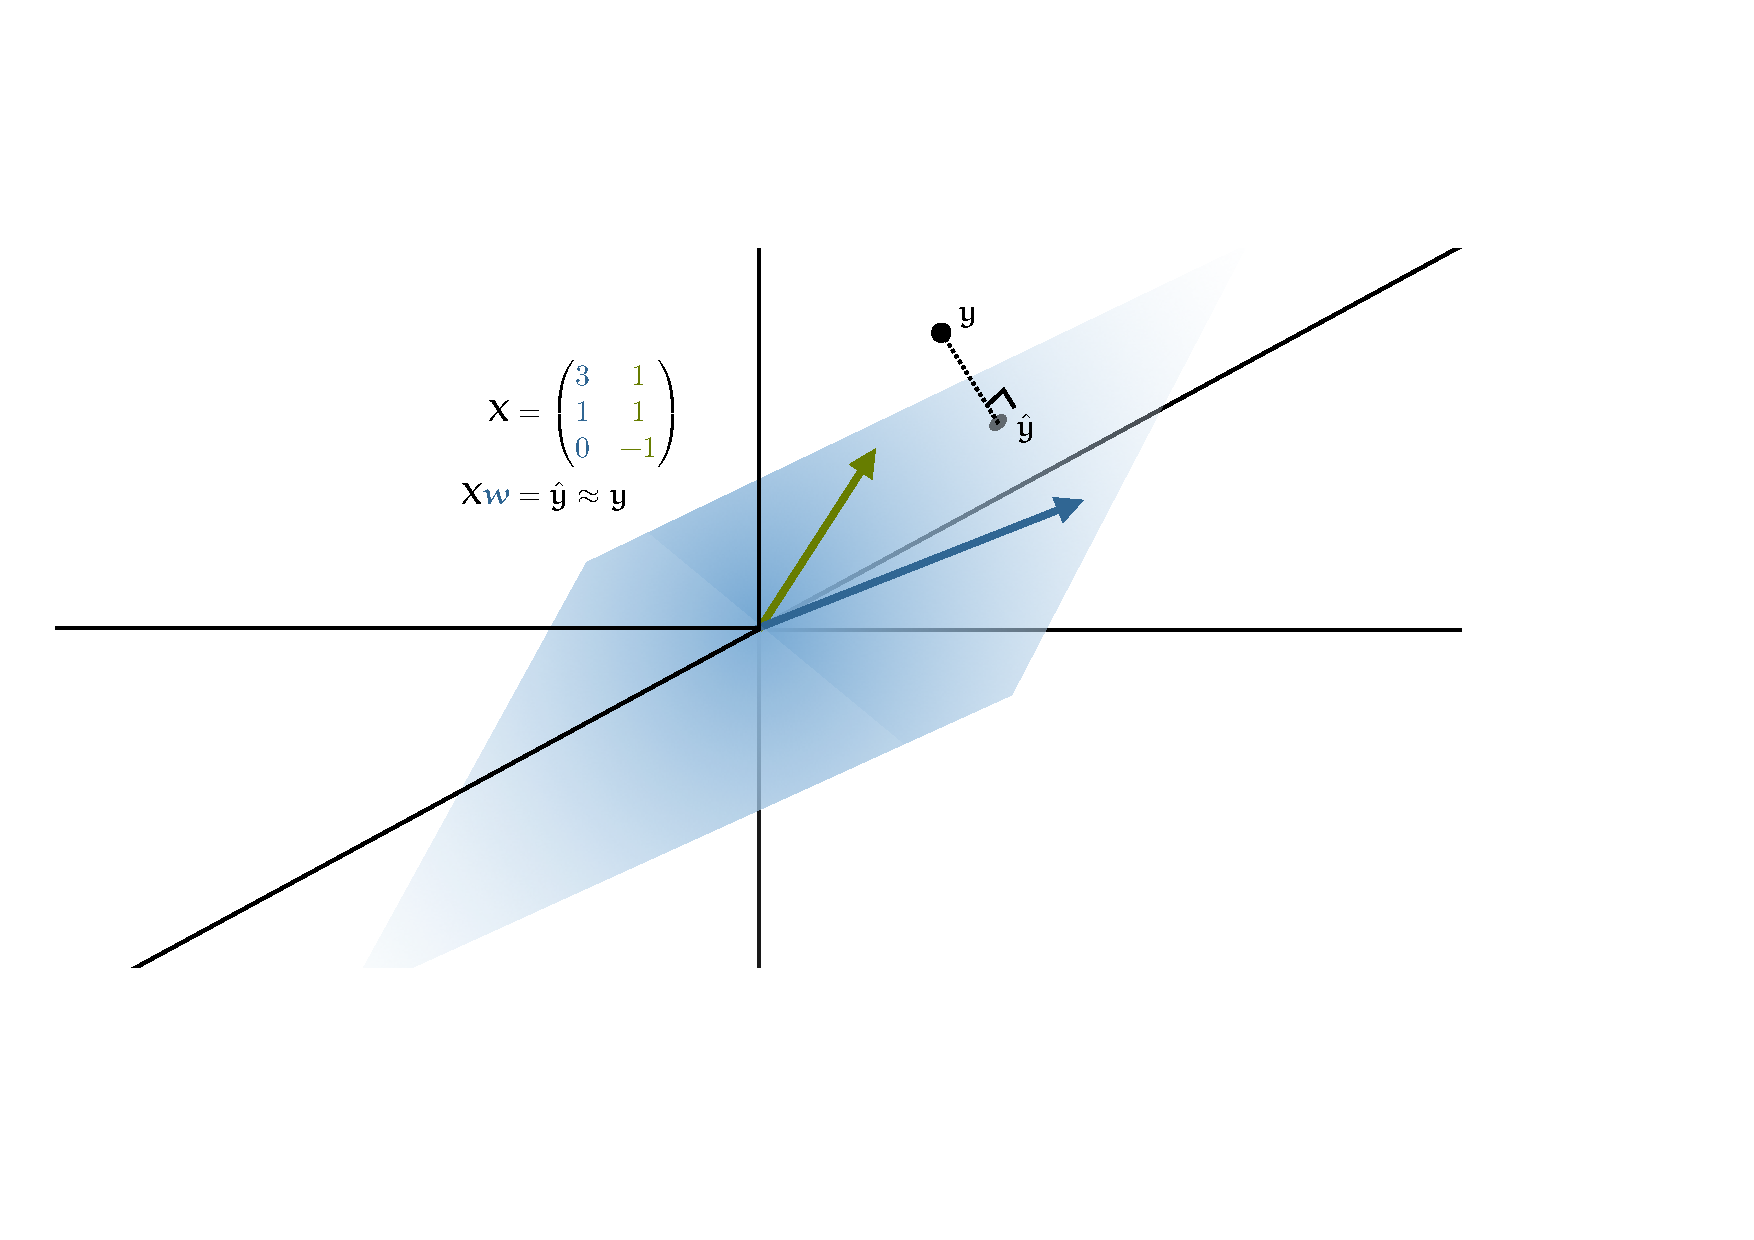
\includegraphics[width=1\textwidth]{./images/pca-4/orth-proj.pdf}
	}
	\caption*{The values \(\mbX\bc{\mbw}\) are constrained to the column space of \(\mbX\), represented by the blue plane. The best solution \(\hat \mby\) to our linear regression problem is the closest we can get to \(\mby\) while staying in the the plane.}
\end{figure}

%<figure class="narrow">
%<img src="/images/pca-4/orth-proj.svg">
%<figcaption>The values \(\X\bc{\w}\) are constrained to the column space of \(\X\), represented by the blue plane. The best solution \(\hat \y\) to our linear regression problem is the closest we can get to \(\y\) while staying in the the plane.
%</figcaption>
%</figure>

\begin{aside}This is a bit of a change of perspective. We are used to visualizing the space \(\mR^m\) where every instance in our dataset is a point in space and every feature is an axis. Now, we're visualizing the space \(\mR^n\), where every feature in our dataset is a point, and every instance is an axis.
\end{aside}

In Chapter~\ref{chapter:introduction}, we saw a simple result called the ``best approximation theorem.'' It stated that if we have a point \(\mbq\) and a line \(\rc{P}\), the closest to \(\mbq\) we can get while staying on the line \(\rc{P}\) is the orthogonal projection of \(q\) onto \(\rc{P}\).

We have a similar situation here. There is a point \(\mby\) that we want to approximate as best we can, but we have to stay in a specific part of space: not a line, but a \emph{subspace}. Specifically the column space of \(\mbX\).

\index{Linear subspace}\index{Subspace!linear}

\begin{aside}A (linear) subspace is a subset of a larger space which contains the origin and for which the linear combination of any two vectors of the subspace is also in the subspace. Aany line, plane or hyperplane that crosses the origin is a subspace. A column space is always a subspace.
\end{aside}


\begin{figure}[H]
	\centerline{
		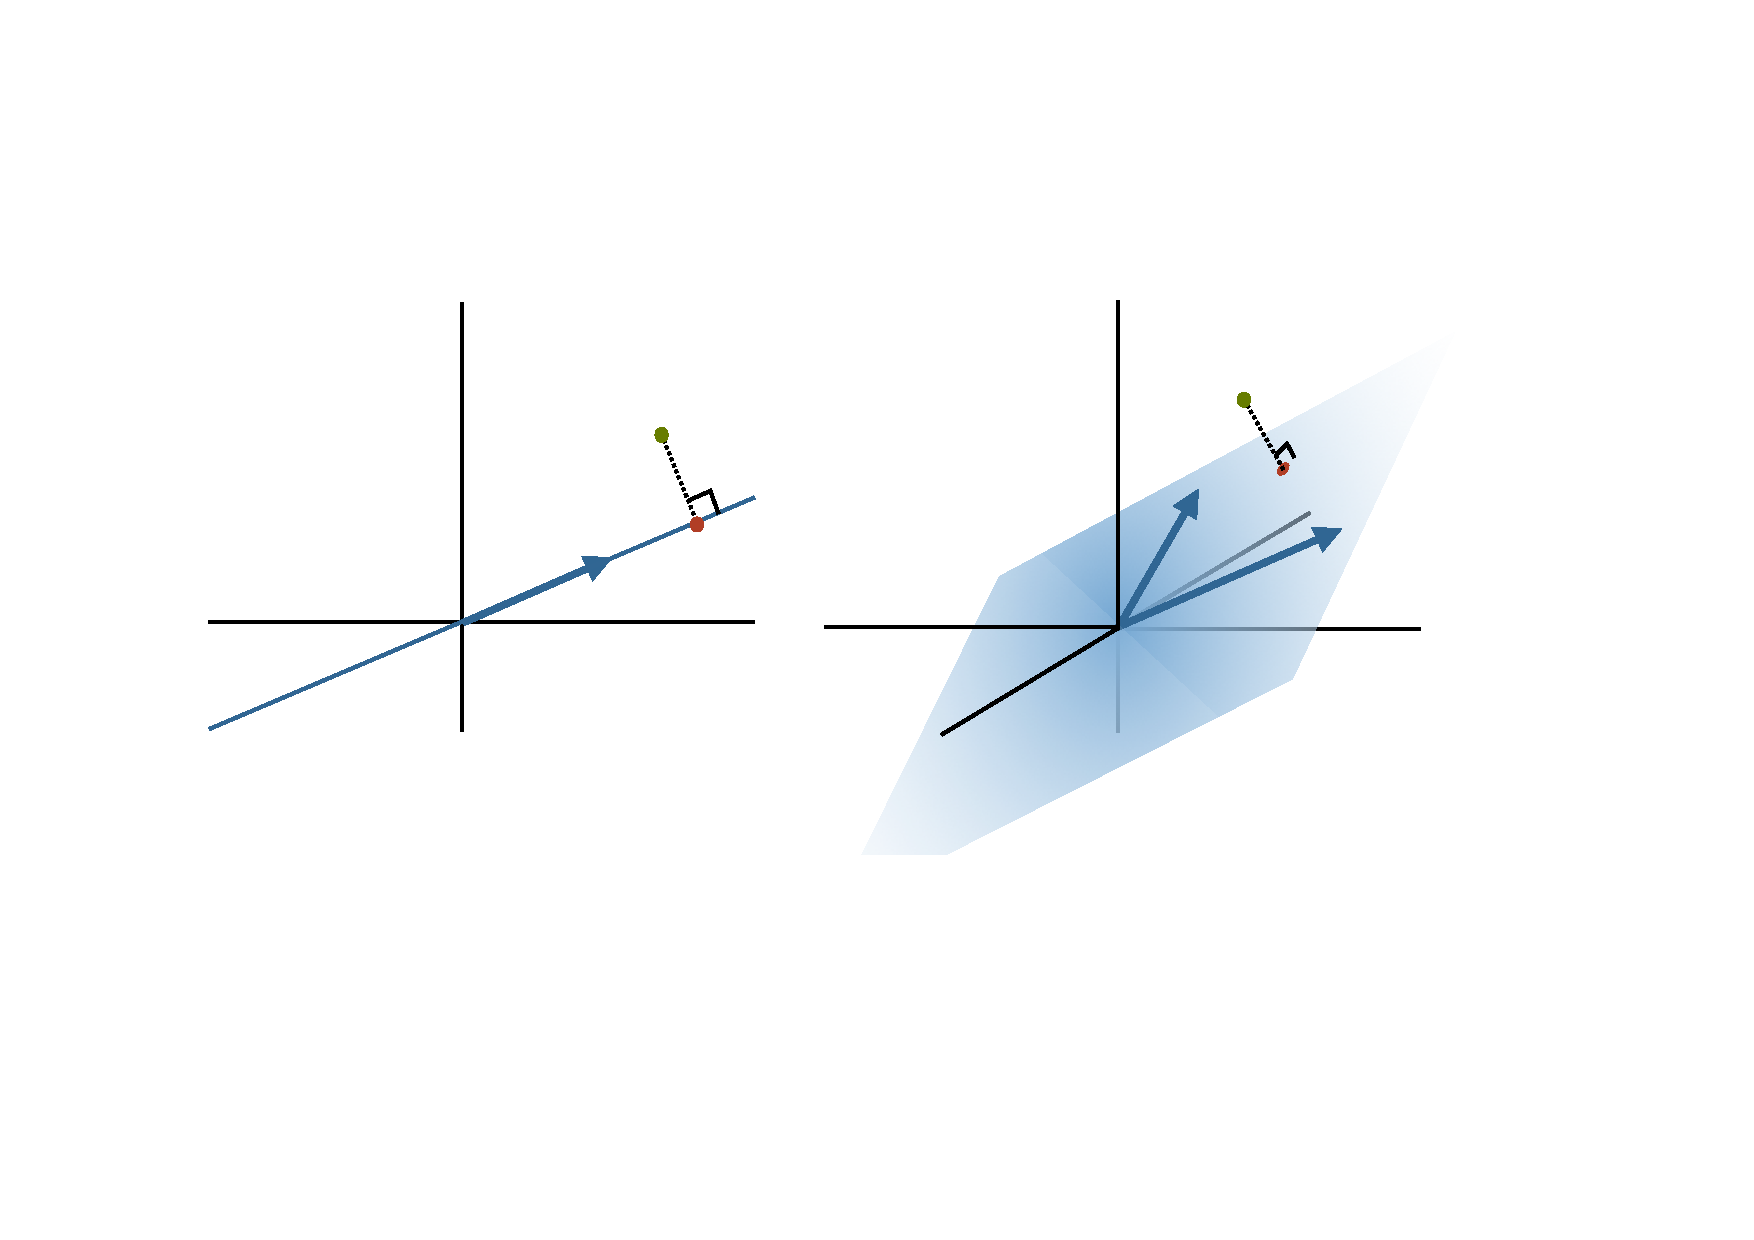
\includegraphics[width=1\textwidth]{./images/pca-4/oned-nd-proj.pdf}
	}
	\caption*{If our subspace is a line, the closest we can get to \gc{any point} is \rc{the orthogonal projection} of that point onto the line. If we define orthogonal projections correctly for \(n\)-dimensional subspaces, like \bc{a plane that crosses the origin}, this principle applies in general.
	}
\end{figure}


%<figure class="narrow">
%<img src="/images/pca-4/oned-nd-proj.svg">
%<figcaption>If our subspace is a line, the closest we can get to <span class="gc">any point</span> is <span class="rc">the orthogonal projection</span> of that point onto the line. If we define orthogonal projections correctly for n-dimensional subspaces, this principle applies in general.
%</figcaption>
%</figure>

Happily, the best approximation theorem holds also when the subspace we're restricted to is more than a line: the closest we can get to a point \(\mbq\) while staying in some subspace \(\rc{S}\) is the orthogonal projection of \(\mbq\) onto \(\rc{S}\). In our case, that means that the best approximation to \(\mby\) within the column space of \(\mbX\) is the orthogonal projection of \(\mby\) onto \(\text{col}\;\mbX\).

The first thing we should do is to define what an orthogonal projection \emph{means} in this context. We'll call a vector orthogonal to a subspace \(\rc{S}\) if it is orthogonal to every vector in \(\rc{S}\). Think of a plane intersecting the origin: a vector orthogonal to the plane points out of the plane at a right angle to every direction in the plane. 

%<!-- <aside>In three dimensions there is only one orthogonal direction, but in higher dimensions, there are infinitely many. If we imagine a line through the origin in a 3D space, the directions orthogonal to it together form a plane.</aside> -->

An orthogonal projection of \(\mbq\) onto \(\rc{S}\) is a point \(\rc{\hat \mbq}\) in \(\rc{S}\) so that the difference vector \(\mbq - \rc{\hat \mbq}\) is orthogonal to \(\rc{S}\). Note how this generalizes the one-dimensional case: the line segment pointing out of the line \(\rc{P}\) at the orthogonal projection is orthogonal to every vector that points along \(\rc{P}\).

Now, we want to show that if we find an orthogonal projection of \(\mbq\) onto \(\rc{S}\), that that is the closest we can get to \(\mbq\) while staying in \(\rc{S}\). We'll follow the same logic as we did in the 1D case. Imagine that we have an orthogonal projection \(\rc{\hat \mbq}\) and any other point \(\rc{\bar \mbq}\) in \(\rc{S}\). No matter how many dimensions our space has, the three points \(\mbq\), \(\rc{\hat \mbq}\) and \(\rc{\bar \mbq}\) form a triangle.

In this triangle, we know that the points \(\rc{\hat \mbq}\) and \(\rc{\bar \mbq}\) are in \(\rc{S}\) so the vector \(\rc{\hat \mbq} - \rc{\bar \mbq}\) must be as well. Because this vector is in \(\rc{S}\), we know that \(\mbq - \rc{\hat \mbq}\) is orthogonal to it so our triangle has a right angle at \(\rc{\hat \mbq}\).


\begin{figure}[H]
	\centerline{
		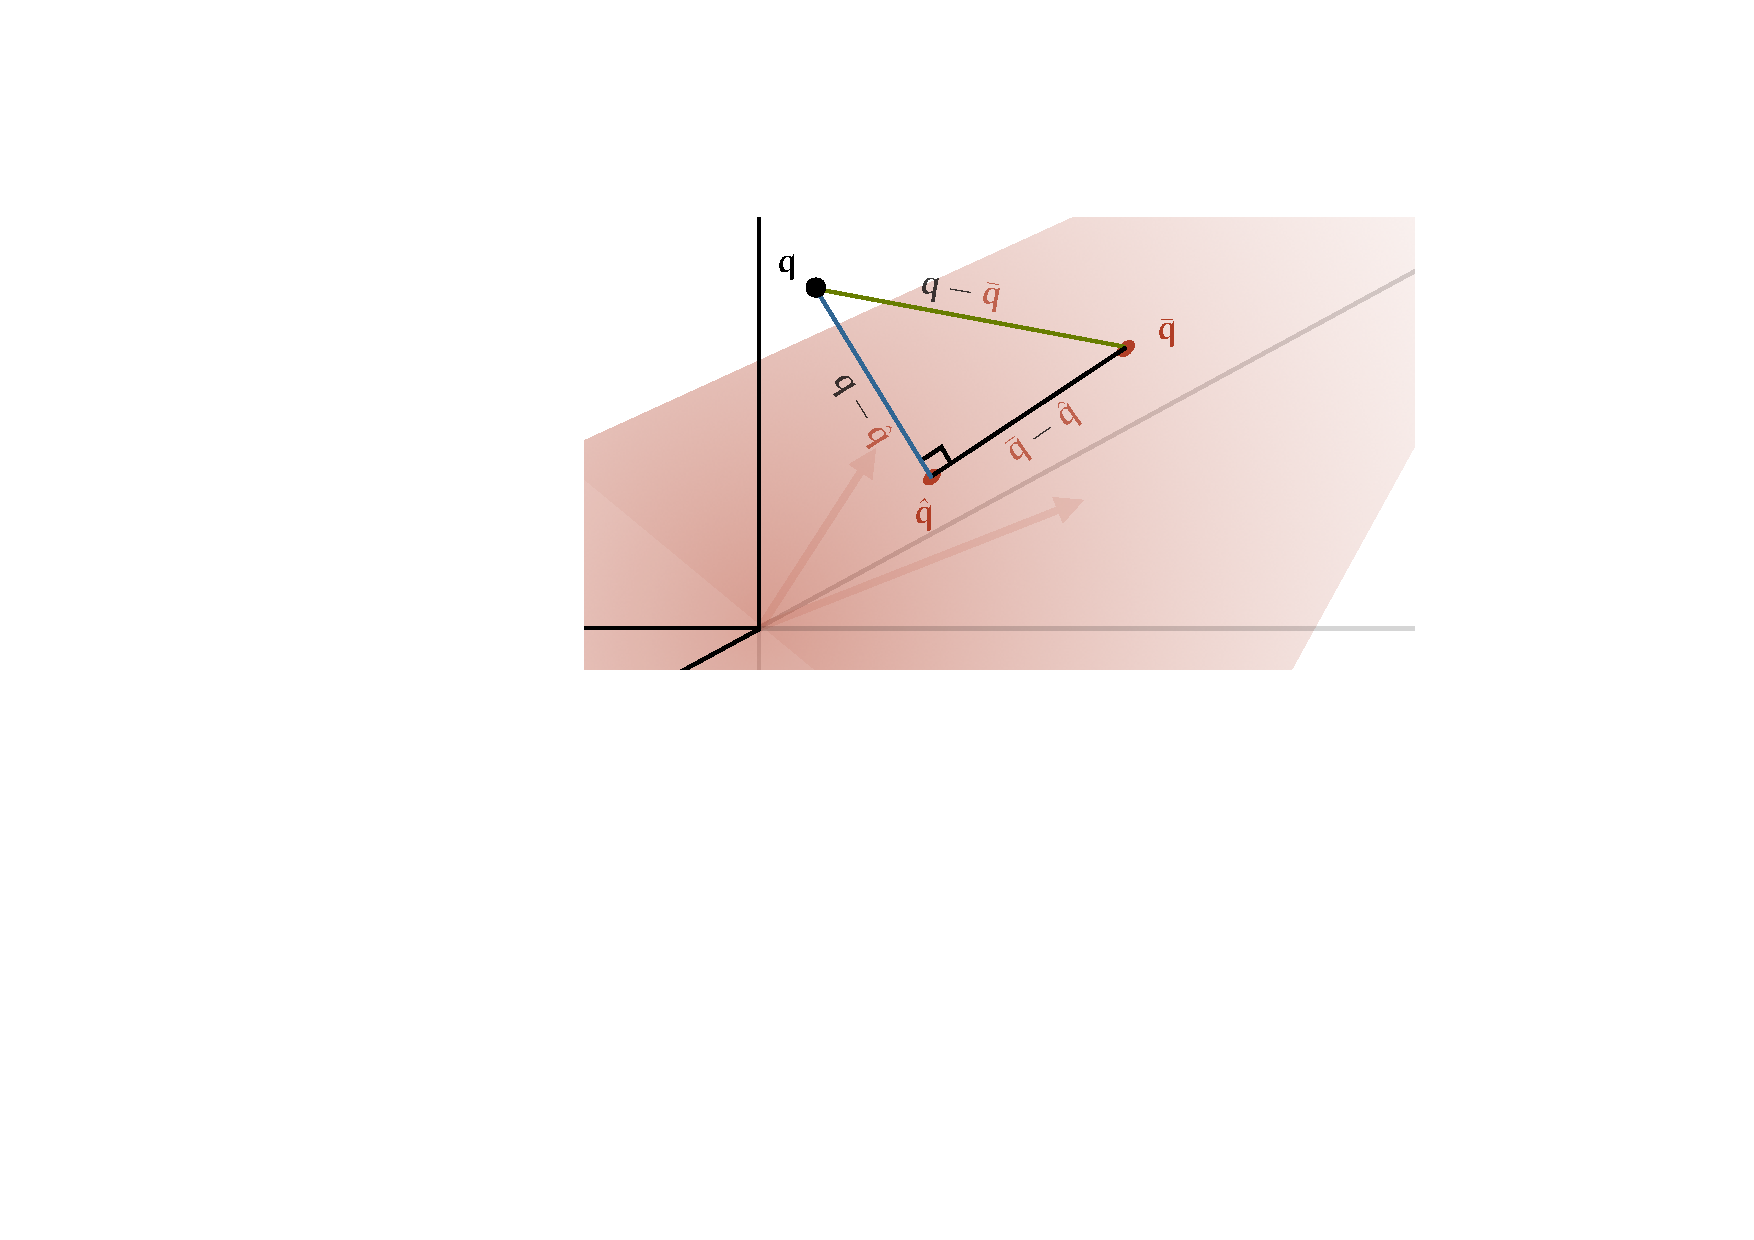
\includegraphics[width=1\textwidth]{./images/pca-4/triangle.pdf}
	}
\end{figure}

%<figure class="narrow centering">
%<img src="/images/pca-4/triangle.png">
%</figure>

From the image, you can already see that the vector \(\bc{\mbq - \hat \mbq}\) must be shorter than or equal to \(\gc{\mbq - \bar \mbq}\). The Pythagorean theorem lets us formalize this:

\[
\|\gc{\mbq - \bar \mbq}\|^2 = \|\hat \mbq - \bar \mbq\|^2 + \|\bc{\mbq - \hat \mbq}\|^2 \p
\]

\index{Pythagorean theorem}

This tells us that the only way \(\rc{\bar \mbq}\) can be as good an approximation as \(\rc{\hat \mbq}\) is if \(\|\rc{\hat \mbq} - \rc{\bar\mbq}\| = 0\), which implies that they are the same vector.

We haven't shown that \(\rc{\hat \mbq}\) exists or that it is unique, but if we can find a set of one or more orthogonal projections of \(\mbq\), they must be the closest we can get to \(\mbq\) while staying inside the subspace \(S\). 

%\enlargethispage{2em}

\begin{aside}As it happens, if \(\rc{S}\) is a proper subspace, and \(\mbq\) is outside it, then there is a unique orthogonal projection \(\rc{\hat \mbq}\). The proof is simple, but we don't need it here.
\end{aside}

Let's return to the problem at hand. We've noted that the predictions our model \(\bc{\mbw}\) can produce for the data \(\mbX\) are restricted to the column space of \(\mbX\). By the argument above, the closest we can get to the target values \(\mby\) is the orthogonal projection of \(\mby\) onto this space. The vector \(\hat \mby = \mbX\bc{\mbw}\) provides an orthogonal projection if the vector \(\oc{\mbe}\) pointing from \(\hat\mby\) to \(\mby\) is orthogonal to the column space of \(\mbX\).

This happens if it is orthogonal to all columns of \(\mbX\). Any vector orthogonal to all columns is also orthogonal to any linear combination of all columns, so it must be orthogonal to \(\text{col}\;\mbX\).

We can phrase this symbolically as

\[
\mbX^T\oc{\mbe} = \mathbf 0
\]

with \(\oc{\mbe} = \mby - \hat \mby\), and \(\mathbf 0\) a vector of zeros. With a bit of filling in and rewriting, we get

%<!-- 
%\[\begin{align*}
%\X^T\left(\y - \X\bc{\w}\right) &= {\mathbf 0} \\
%\y^T\X - \X^T\X\bc{\w} &= {\mathbf 0} \\
%\X^T\X\bc{\w} &= \X^T\y \\
%\end{align*}\]
% -->

\begin{align*}
\mbX^T\left(\mby - \hat\mby\right) &= {\mathbf 0} \\
\mbX^T\mby  &= \mbX^T\hat\mby \\
\mbX^T\mby &= \mbX^T\mbX\bc{\mbw} \\
\end{align*}

\index{Normal equation}

This is called the \textbf{normal equation} for our linear problem. Any \(\bc{\mbw}\) that satisfies this equation is a least squares solution. Note that \(\mbX^T\mbX\) has popped up again.

In fact, we can see here that \textbf{if \(\mbX^T\mbX\) is invertible}, we can multiply both sides by the inverse and get

\[\left (\mbX^T\mbX\right)^{-1}\mbX^T\mby = \bc{\mbw}\]

as a single, unique solution for \(\bc{\mbw}\).

%<!--  When is this the case? We saw earlier that a square matrix is invertible if and only if it is full-rank. That means that the \(m\) rows of \(\X^T\X\) need to be linearly independent. -->

\index{Pseudo-inverse|textbf}

The term \(\left (\mbX^T\mbX \right)^{-1}\mbX^T\) is an instance of something called the \textbf{pseudo-inverse} of \(\mbX\), written \(\mbX^\dagger\). We'll provide a more robust definition later, but it's interesting to see where the name comes from. Think back to the idealized version of our problem \(\mbX\bc{\mbw} = \mby\). When we are lucky enough to have a square and full-rank \(\mbX\), we can compute the exact solution by multiplying both sides by the inverse of \(\mbX\): \(\bc{\mbw} = \mbX^{-1}\mby\). We take the multiplier ``to the other side'' just like we would do with a scalar equation. General rectangular matrices don't have an inverse, but when we replace it by the pseudo-inverse, we get the least-squares solution, which will coincide with the ideal solution if one exists.

\begin{aside}In fact, if \(\mbX\) is invertible, \(\mbX^\dagger\) coincides with the inverse, because, from basic properties of the inverse we get \(\small (\mbX^T\mbX)^{-1}\mbX^T = \mbX^{-1}{\mbX^T}^{-1}\mbX^T = \mbX^{-1}\).
\end{aside}

Note that if \(\mbX\) has dimensions \(\gc{n} \times \bc{m}\), then \(\mbX^\dagger\) has dimensions \(\bc{m} \times \gc{n}\). This is consistent with the idea that if \(\mbX\) represents a function from \(\mR^\bc{m}\) to \(\mR^\gc{n}\), then something analogous to its inverse should represent a function from \(\mR^\gc{n}\) to \(\mR^\bc{m}\)

What happens if \(\mbX^T\mbX\) is not invertible? It turns out this this happens precisely when the rank of \(\mbX\) is strictly less than the number of columns. One such case is if \(\mbX\) is wider than it is tall, like the dataset of portrait images we saw in Chapter~\ref{chapter:introduction}. This makes sense if you think back to the ideal solution to our problem: \(\mbX\bc{\mbw} = \mby\). If \(\mbX\) is wider than it is tall (and full-rank) then this is a system of \({n}\) equations with \({m}\)  variables: we will get many different solutions.
%
%<!-- <aside>Another way we can have a lower rank than \(m\) is if the matrix is taller than it is wide, but most rows aren't linearly independent. We'll see an example of this in a bit.</aside> -->

We can prove this fact simply from the SVD. This is a good illustration of how the SVD can be used for theoretical purposes. What we want to show is that if \(\mbX^T\mbX\) is non-invertible, \(\mbX\) must have a column rank less than \(\bc{m}\). Let \(k < {m}\) be the rank of \(\mbX\) and let

\[\mbX = \rc{\mbU}_{m}\gc{\Sig}_{m}{\rc{\mbV}_{m}}^T\]

be the SVD of \(\mbX\) truncated at \(\bc{m}\). Note that we only have \(k\) singular values so some of the diagonal of \(\gc{\Sig}_\bc{m}\) is zero. Note also that the columns of \(\rc{\mbV}_\bc{m}\) have length \(\bc{m}\), so \(\rc{\mbV}_\bc{m}\) is square.

\pagebreak \noindent With this decomposition, we can write
\begin{align*}
\mbX^T\mbX &= \rc{\mbV}_m{\gc{\Sig}_m}^T{\rc{\mbU}_m}^T\rc{\mbU}_m\gc{\Sig}_m{\rc{\mbV}_m}^T \\
	   &= \rc{\mbV}_m{\gc{\Sig}_m}^2{\rc{\mbV}_m}^T
\end{align*}
where the \(\rc{\mbU}_m\)'s in the middle disappear, because \(\rc{\mbU}_m\)'s columns are orthogonal to one another, so together they form an identity matrix. Note also that \(\gc{\Sig}_m\) is diagonal, so it's equal to its transpose and multiplying it by itself boils down to squaring the diagonal values.

The resulting decomposition is equal to the eigendecomposition of \(\mbX^T\mbX\), which we already knew existed. However, what we've now shown as well, is that because \(\mbX\) has lower rank than \(m\), \emph{some of its eigenvalues are zero}. We know that \(\rc{\mbV}_m\) and \({\rc{\mbV}_m}^T\) are orthogonal, so they are invertible. 

\index{Eigendecomposition}

The composition of invertible matrices is invertible, so whether \(\mbX^T\mbX\) is invertible boils down to whether \({\gc{\Sigma}_m}^2\) is invertible. A diagonal matrix with only \emph{non}zero values on the diagonal is invertible: when we multiply a vector by it, we multiply each element of the vector by one of the diagonal elements, so we can get back the original elements by multiplying by their inverses. However, a diagonal matrix with a zero anywhere on the diagonal is singular. We lose information if we multiply by it, because those elements of the input vector that were multiplied by zero cannot be recovered from the output vector.

\index{Invertibility!of diagonal matrices}

That means that if \(\mbX\) has rank \(m\), \({\gc{\Sig}}^2\) must have \(m\) non-zero diagonal values, i.e. \(\mbX^T\mbX\) must be invertible. If the rank of \(\mbX\) is less than \(m\), we get fewer nonzero values on the diagonal of \({\gc{\Sig}}^2\), and \(\mbX^T\mbX\) is singular.
%
%<!-- 
%<aside>To prove the other direction: that \(\X^T\X\) being invertible implies that \(\X\) has rank \(m\), start with its eigendecomposition, and note that we know all eigenvalues are positive, so have squares. If \(\X^T\X\) is invertible, we have \(m\) nonzero eigenvalues, which we can use to construct an SVD with at least \(m\) eigenvectors. If \(\X^T\X\) is singular, we can show that there must be one zero eigenvalue, and therefore strictly less than \(m\) singular values.
%</aside>
% -->

\index{Pseudo-inverse! for singular \(\mbX^T\mbX\)}

What should we do when \(\mbX^T\mbX\) is singular? This means we have multiple exact solutions to our problem \(\mbX\bc{\mbw} = \mby\), so we need an additional constraint to choose a single one. One common heuristic in machine learning is to pick models for which the parameter values are small. The simplest option is to pick the \(\bc{\mbw}\) that satisfies \(\mbX\bc{\mbw} = \mby\) for which \(\|\bc{\mbw}\|\) is minimal.

One of the most beautiful properties of the pseudo-inverse is that if we define it carefully, it automatically delivers this solution if multiple solutions are available.

To show this, we will investigate what happens if we add a small invertible matrix to \(\mbX^T\mbX\) to make it invertible. Specifically, we'll add a small multiple \(\oc{\epsilon}\) of the identity matrix. Doing this, the normal equation becomes

\[
\left (\mbX^T\mbX + \oc{\epsilon}\mbI \right )\bc{\mbw} = \mbX^T\mby \p
\]

The idea is that we can let \(\oc{\epsilon}\) go to zero to see which solution the pseudo-inverse gives us.

To see why \(\mbX^T\mbX + \oc{\epsilon}\mbI\) must be invertible, consider the vectors represented by its columns. If \(\mbX^T\mbX\) is singular, and thus rank deficient, these must all lie in some subspace of lower dimension than \(m\). By adding \(\oc{\epsilon}\mbI\), we are pulling each vector a little bit in the direction of a \emph{different} axis. Imagine two vectors on the same line. If I pull one a little toward the horizontal, and the other a little toward the vertical, they must both leave the line they originally had in common. 

\begin{figure}[H]
	\centerline{
		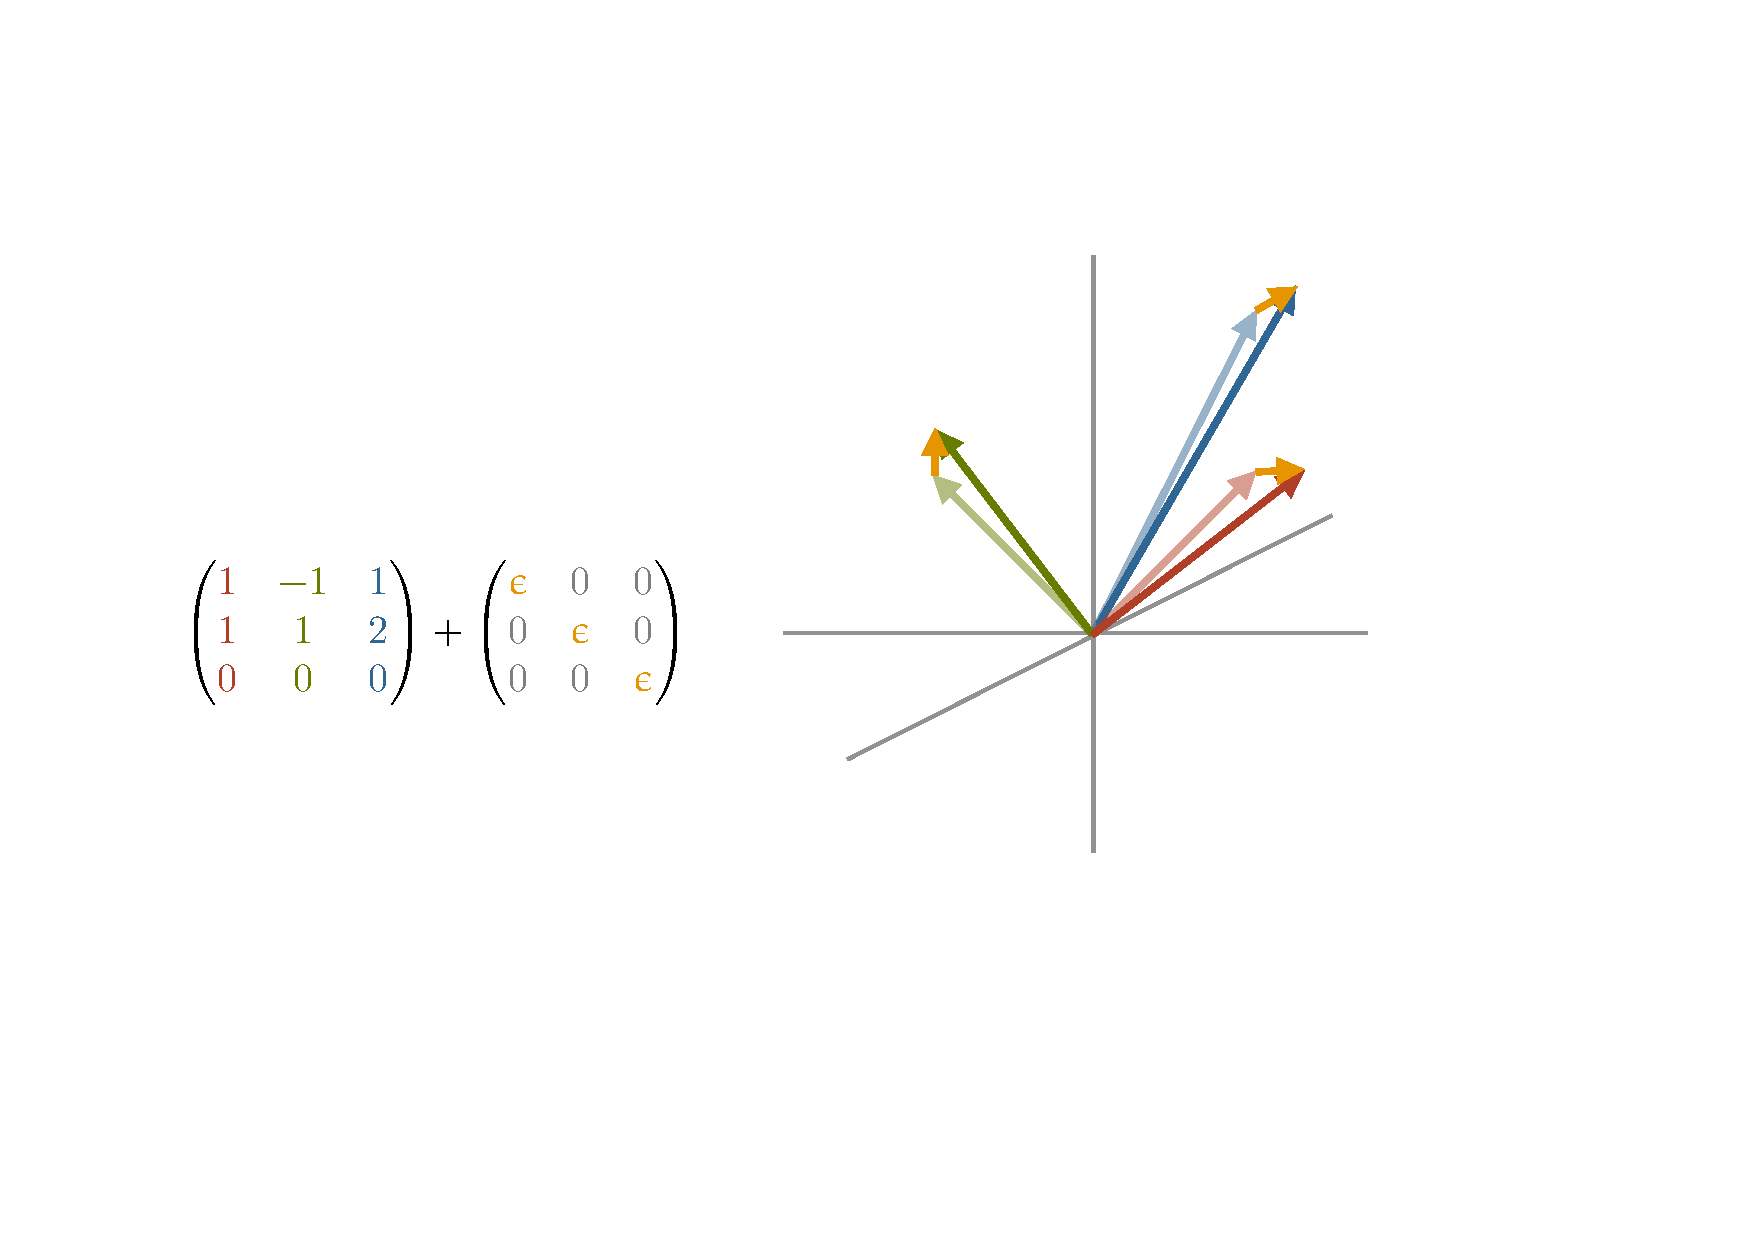
\includegraphics[width=1\textwidth]{./images/pca-4/nudge.pdf}
	}
	\caption*{Adding a matrix \(\oc{\epsilon}\mbI\) to a low-rank matrix, nudges each column vector of the original by \(\oc{\epsilon}\) in the direction one of the axes, making the matrix full rank.
	}
\end{figure}

%<figure class="narrow centering">
%<img src="/images/pca-4/nudge.svg">
%<figcaption>Adding a matrix \(\oc{\epsilon}\I\) to a low rank matrix, nudges each column vector of the original by \(\oc{\epsilon}\) in the direction one of the axes, making the matrix full rank.
%</figcaption>
%</figure>

We can now rewrite our modified normal equation as

\begin{align*}
\mbX^T\mbX\bc{\mbw} = \mbX^T\mby - \oc{\epsilon}\bc{\mbw} \p
\end{align*}

To get some insight into what the solutions to this equation look like, let's imagine that we have an \(n \times 2\) data matrix (\(n\) instances, \(2\) features) and that the first column of \(\mbX\) happens to be a unit vector, and the second column is twice the first column. This gives us

\[\mbX^T\mbX = \begin{pmatrix}1 & 2 \\ 2 & 4 \end{pmatrix}\p\]

<p>This is a singular matrix: the second column is twice the first. Its operation is to squeeze the whole plane into a single line. Any \(\bc{\mbw}\) is mapped to a point \((\rc{x}, 2\rc{x})\), with \(\rc{x} = \bc{w}_1 + 2\bc{w_2}\).

\begin{figure}[H]
	\centerline{
		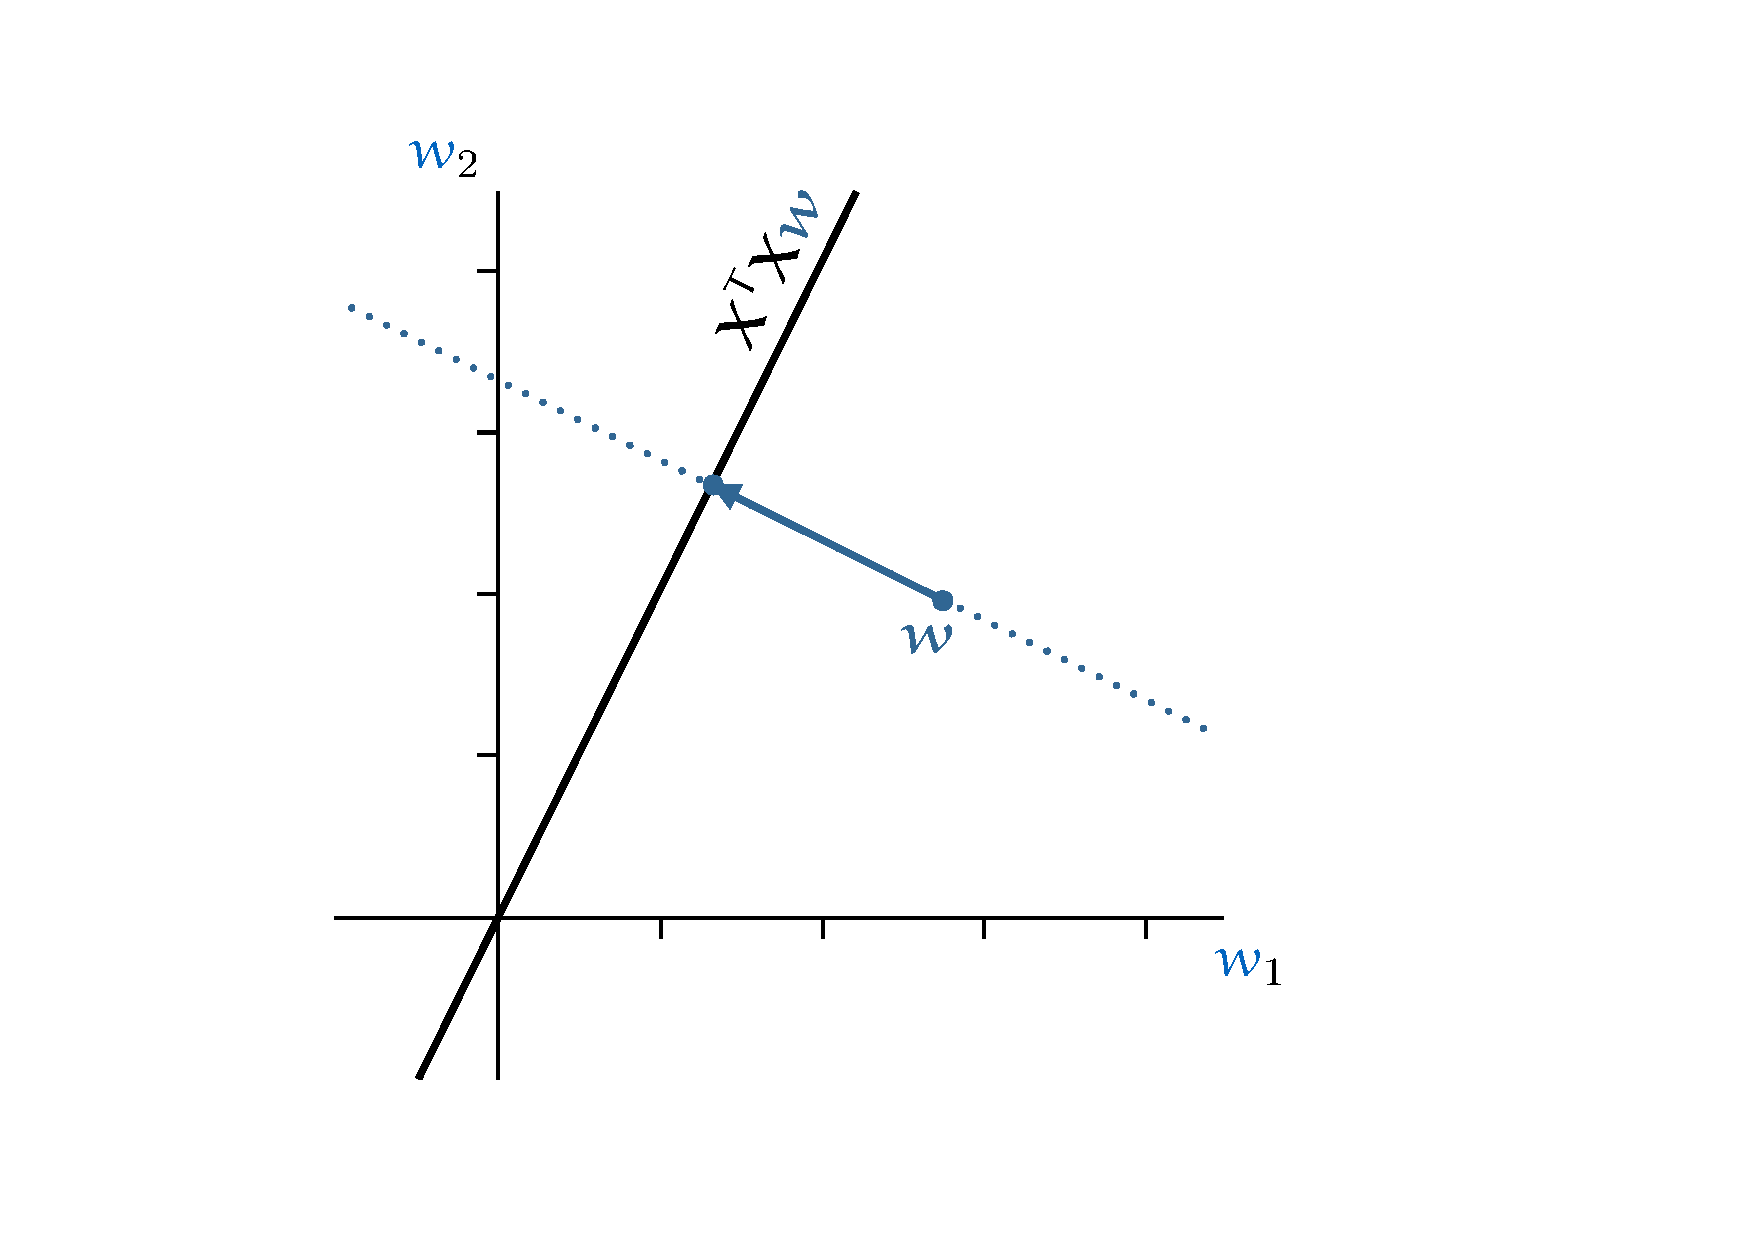
\includegraphics[width=0.6\textwidth]{./images/pca-4/projection.pdf}
	}
	\caption*{The low-rank matrix \(\mbX^T\mbX\) projects multiple points \(\bc{\mbw}\) onto the same point in its column space. In this case, a line of points is projected to a single point on the line \(\bc{w}_1 = 2\bc{w}_2\).

	}
\end{figure}

%<figure class="narrow centering">
%<img src="/images/pca-4/projection.svg" class="three-quarters">
%<figcaption>The low-rank matrix \(\X^T\X\) projects multiple points \(\bc{\w}\) onto the same point in its column space. In this case, a line of points is projected to a single point on the line \(\bc{w}_1 = 2\bc{w}_2\)
%</figcaption>
%</figure>


\index{Pre-image|textbf}

The line of all points mapped to \((\rc{x}, 2\rc{x})\), its \emph{pre-image}, is orthogonal to the line that forms the column space. In this specific instance, we can rewrite \(\bc{w}_2 = -\frac{1}{2}\bc{w}_1 \kc{+ \frac{1}{2}x}\). That is, a line with slope \(-\frac{1}{2}\), which we can tell by inspection is orthogonal to our line with slope \(2\). But this is not just true in this instance, it holds more generally. For any matrix \(\gc{\mbM}\), the pre-image of some point in \(\text{col } \gc{\mbM}\) is orthogonal to the column space itself.
\enlargethispage{2em}

\begin{aside}See the appendix for a proof.\end{aside}

The original normal equation states that we want to choose \(\bc{\mbw}\) so that \(\mbX^T\mbX\bc{\mbw}\) coincides with the point \(\mbX^T\mby\). Since the second column of \(\mbX\) is twice the first, we have 

\[\mbX^T\mby = \begin{pmatrix}y' \\ 2 y'\end{pmatrix}\]

for some \(y'\). This is on the line that corresponds to \(\text{col } \mbX^T\mbX\). Every \(\bc{\mbw}\) for which \(\bc{w}_1 + 2\bc{w}_2 = y'\), will be mapped onto this point giving us a solution for \(\mbX^T\mbX\bc{\mbw} = \mbX\mby\).


%<!-- 
%Since the second column of \(\X\) is twice the first, \(\X^T\y\) will always be a vector with the second element twice as big as the first, whatever \(\y\) is. 
% -->
%
%<!-- 
%Since the second _row_ of \(\X^T\X\) is also twice the first, the same property holds for the result of \(\X^T\X\bc{\w}\), whatever \(\bc{\w}\) is. Both sides will lie on the line \(x = 2y\). More importantly, this means that the matrix \(\X^T\X\) squishes a 2D space into a 1D space. A whole line of points is being mapped to the point \(\X^T\y\). Any point on this line is a solution to the normal equation.
% -->

\begin{figure}[H]
	\centerline{
		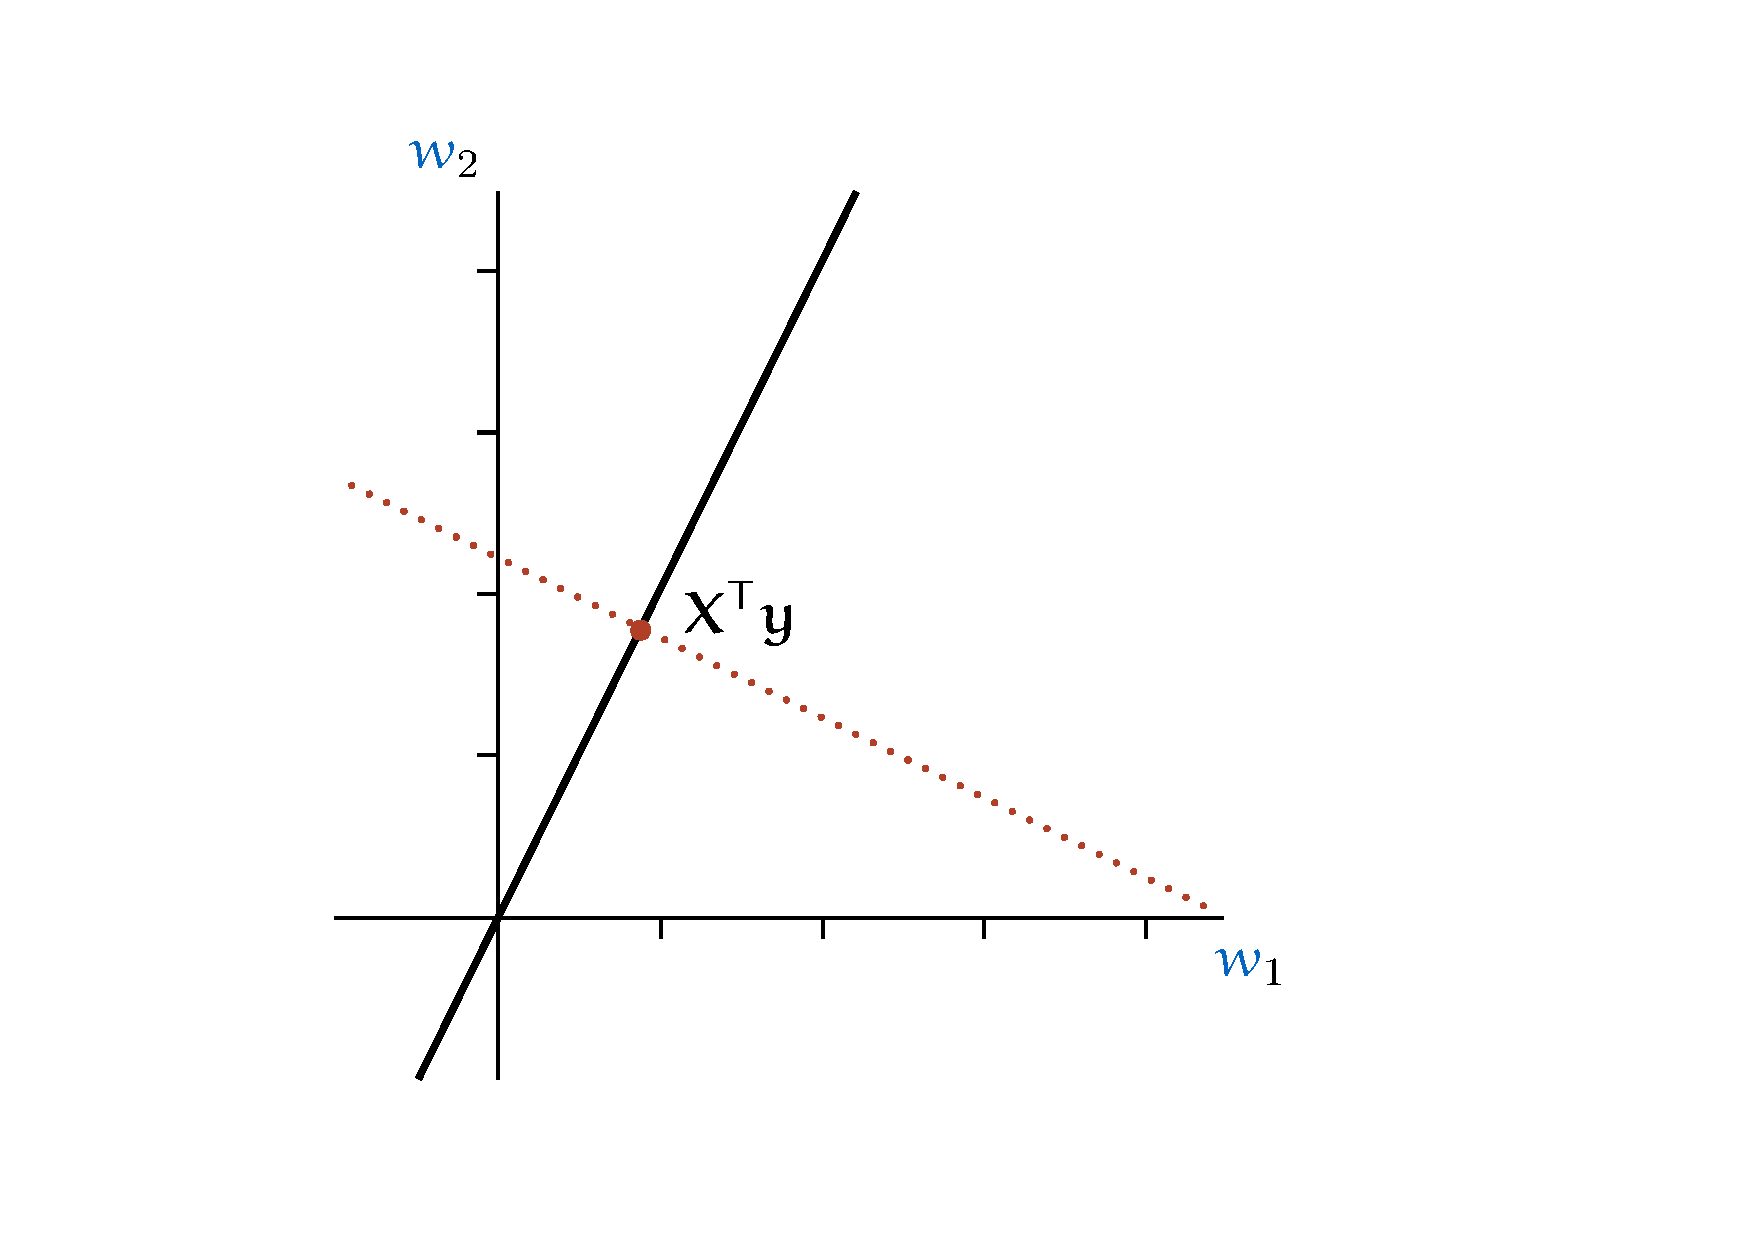
\includegraphics[width=0.6\textwidth]{./images/pca-4/projection-target.pdf}
	}
	\caption*{Given our target \(\mby\), we note that \(\mbx^T\mby\) is in the column space of \(\mbX^T\mbX\), and its pre-image forms an orthogonal line. Here we see the effect of an overdetermined problem: we have multiple solutions to the normal equation.
	}
\end{figure}

%<figure class="narrow centering">
%<img src="/images/pca-4/projection-target.svg" class="three-quarters">
%<figcaption>Given our target \(\y\), we note that \(\x^T\y\) is in the column space of \(\X^T\X\), and its pre-image forms an orthogonal line. Here we see the effect of an overdetermined problem: we have multiple solutions to the normal equation.
%</figcaption>
%</figure>

Now, when we introduce the term \(\oc{\epsilon}\bc{\mbw}\) to the left-hand-side. This moves our target by a small multiple of \(\bc{\mbw}\). Where formerly we got from \(\bc{\mbw}\) to the target \(\mbX^T\mby\) in a single matrix multiplication, we now need two steps: first we multiply \(\mbX^T\mbX\bc{\mbw}\) and then we add \(\oc{\epsilon}\bc{\mbw}\). The first step is guaranteed to put us in the column space of \(\mbX^T\mbX\), which is where the target is as well. Therefore, if we are going to reach the target, the second step should keep us in the column space. In other words, \(\bc{\mbw}\) needs to point along the column space.

\begin{figure}[H]
	\centerline{
		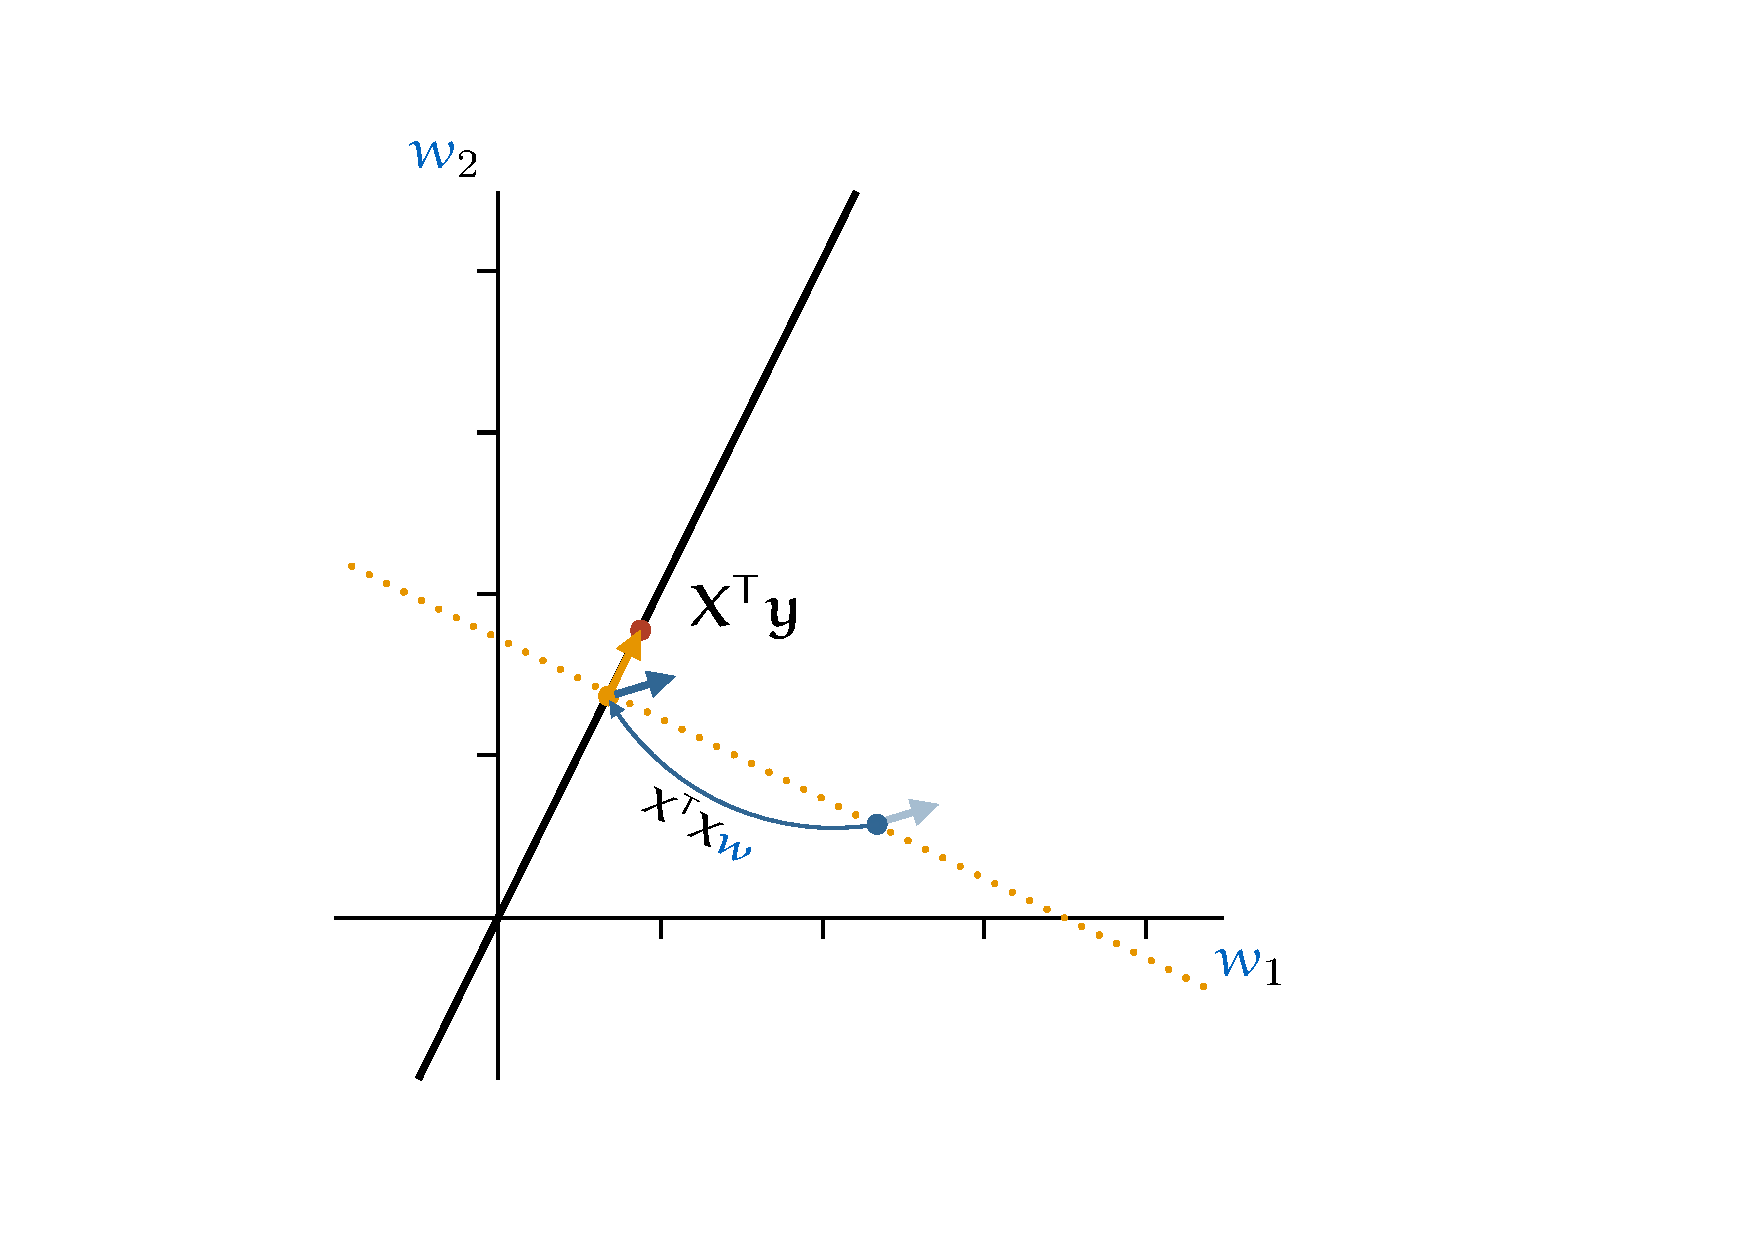
\includegraphics[width=0.6\textwidth]{./images/pca-4/projection-fin.pdf}
	}
	\caption*{After we change the normal equation to \(\mbX^T\mbX\bc{\mbw} + \oc{\epsilon}\bc{\mbw} = \mbX^T\mby\), we need an extra step to get to the target. The projection onto the column space should end slightly below \(\mbX^T\mby\) so that the term \(+\oc{\epsilon}\bc{\mbw}\) can take us to the target. We then see that only one point on the dotted line will do the trick: if we use the blue point, the second step will push us out of the column space. Only the \(\bc{\mbw}\) corresponding to the direction of the column space will allow the final step to actually reach \(\mbX^T\mby\).
	}
\end{figure}

%<figure class="narrow centering">
%<img src="/images/pca-4/projection-fin.svg" class="three-quarters">
%<figcaption>After we change the normal equation to \(\X^T\X\bc{\w} + \oc{\epsilon}\bc{\w} = \X^T\y\), we need an extra step to get to the target. The projection onto the column space should end slightly below \(\X^T\y\) so that the term \(+\oc{\epsilon}\bc{\w}\) can take us to the target. We then see that only one point on the dotted line will do the trick: if we use the blue point, the second step will push us out of the column space. Only the \(\bc{\w}\) corresponding to the direction of the column space will allow the final step to actually reach \(\X^T\y\).
%</figcaption>
%</figure>

This is how the term \(\oc{\epsilon}\bc{\mbw}\) moves us from a problem with multiple solutions a problem with a single solution. We've also claimed that this solution is the one with the smallest norm. How do we see this in the image? The trick is to note that the the line \(\oc{P}\) from which we choose \(\bc{\mbw}\) is orthogonal to the column space, which crosses the origin. This means that if we choose the point where the two cross, we are essentially \emph{projecting the origin onto \(\oc{P}\)}. This means we've chosen the point on \(\oc{P}\) that is \emph{closest} to the origin, or, in other words, the solution with the smallest norm.

We've ignored the fact that we changed the target by the term \(\oc{\epsilon}\mbI\), so we've slightly changed the problem. But we can justify that by making \(\oc{\epsilon}\) very small. The whole derivation still holds, so long as it's non-zero. More technically, as we let \(\oc{\epsilon}\) go to zero, our solution converges to the one with the lowest L2 norm.

This is a very neat principle, which we'd like to work into our definition of the pseudo-inverse. To this end, we can define \(\mbX^\dagger\) as the matrix

\[
\mbX^\dagger = \lim_{\oc{\epsilon} \to 0}\left(\mbX^T\mbX + \oc{\epsilon}\mbI \right)^{-1}\mbX^T \p
\]

\index{Pseudo-inverse!definition}
\index{$\gc{\mbM}^\dagger$}

That is, if the inverse of \(\mbX^T\mbX\) exists, we simply use it as before, but if it doesn't, we instead use the matrix that is the limit of \(\mbX^T\mbX + \oc{\epsilon}\mbI\) for ever smaller \(\oc{\epsilon}\). In the context of our least squares problem, the limit adds an extra constraint so that we converge to the approximation to the inverse that will give us the solution with the smallest norm.

That was a long story, so let's recap:
\begin{itemize}
\item The pseudo-inverse lets us solve matrix equations. Whenever you feel like moving a matrix to the other side by taking its inverse, but the inverse doesn't exist, you can use the pseudo-inverse instead.
\item This will give you an exact solution if one exists, and a least squares solution if it doesn't.
\item If multiple solutions exist, you'll get the one with the smallest norm.
\end{itemize}

\index{Pseudo-inverse!properties of}

So, all in all, the pseudo-inverse is a pretty powerful tool. How do we compute it? Obviously, if we know that \(\mbX\) has full column rank, we can just compute \(\mbX^T\mbX\), take its inverse, and multiply by \(\mbX^T\). But that isn't always the nicest approach. For one thing, computing the inverse is a numerically unstable business. In fact you usually avoid it by computing the pseudo-inverse instead, even if the inverse exists. Another problem is that this only works for \(\mbX\) with full column-rank. Ideally, we would have a single, simple algorithm that returns the limit version of the pseudo-inverse if \(\mbX^T\mbX\) isn't invertible, without us having to check.

As you may have guessed, one of the best ways of achieving this is by the singular value decomposition.

\index{Pseudo-inverse!computing by SVD}

\pagebreak\noindent The algorithm is simple, so let's start there, and show why it's correct later. Given \(\mbX\), we first compute its SVD

\[\mbX = \rc{\mbU}\gc{\Sig}\rc{\mbV}^T \p\]

On the diagonal of \(\gc{\Sig}\), replace all non-zero values \(\gc{\sigma}\) by their inverse \(1/\gc{\sigma}\), and call the resulting matrix \(\gc{\Sig}^\dagger\). We then reverse the basis transformations, and the result is the pseudo-inverse:

\[\mbX^\dagger = \rc{\mbV}\gc{\Sig}^\dagger\rc{\mbU}^T \p\]

\begin{aside}Note that this also directly provides us with an SVD of \(\mbX^\dagger\).
\end{aside}

If we don't want to compute the full SVD, we get the same result with the truncated SVD, so long as we include all singular values.

\begin{aside}This is because the \(\rc{\mbv}\) and \(\rc{\mbu}\) vectors corresponding to the \(\mathbf 0\) block of \(\gc{\Sig}\) can be safely removed without changing the value of the decomposition. We haven't modified these vectors when we computed \(\mbX^\dagger\), so the result isn't changed if we don't include these.\end{aside}

The main reason that the SVD is the preferred way of computing the pseudo-inverse is one we've seen before: noise. In fact, noise can be particularly disastrous when we compute the pseudo-inverse. A small amount of noise turns zero singular values into very small non-zero singular values. We can see above that they become very \emph{big} singular values in the pseudo-inverse because we take their inverse, when actually they should be ignored. In short, a small amount of noise in \(\mbX\) creates a huge error in  \(\mbX^\dagger\). The SVD makes this process explicit, and allows us to simply treat very small singular values as zero, eliminating the problem.

Now, why does this algorithm give us the pseudo-inverse? Let's first look at the case where \(\mbX\) has full column rank \(m\). In that case, the pseudo-inverse is simply:

\[\mbX^\dagger = \left( \mbX^T\mbX\right)^{-1}\mbX^T
\]

Replacing each \(\mbX\) by its SVD, truncated to \(m\) and omitting the subscripts to simplify the notation, we get

\begin{align*}
\mbX^\dagger &= \left( \rc{\mbV}\gc{\Sig}\rc{\mbU}^T \rc{\mbU}\gc{\Sig}\rc{\mbV}^T \right)^{-1} \rc{\mbV}\gc{\Sig}\rc{\mbU}^T \\
&= \left( \rc{\mbV}\gc{\Sig}^2\rc{\mbV}^T \right)^{-1} \rc{\mbV}\gc{\Sig}\rc{\mbU}^T\\
&= \rc{\mbV}\gc{\Sig}^{-2}\rc{\mbV}^T \rc{\mbV}\gc{\Sig}\rc{\mbU}^T\\
&= \rc{\mbV}\gc{\Sig}^{-1}\rc{\mbU}^T \p
\end{align*}

Which is the result of the algorithm described above. Note that because we truncated at \(m\), \(\gc{\Sig}\) and \(\rc{\mbV}\) are \( m \times m\).

To make it intuitive exactly how SVD is solving our problem here, we can return to an idea we used before when we were developing eigenvectors: everything is a lot easier when your matrices are diagonal. Let's try that here. Imagine that \(\mbX\) is a diagonal \(n \times n\) matrix and we are looking for the vector \(\bc{\mbw}\) that minimizes the distance between \(\mbX\bc{\mbw}\) and a given \(\mby \in \mR^n\).

\begin{figure}[H]
	\centerline{
		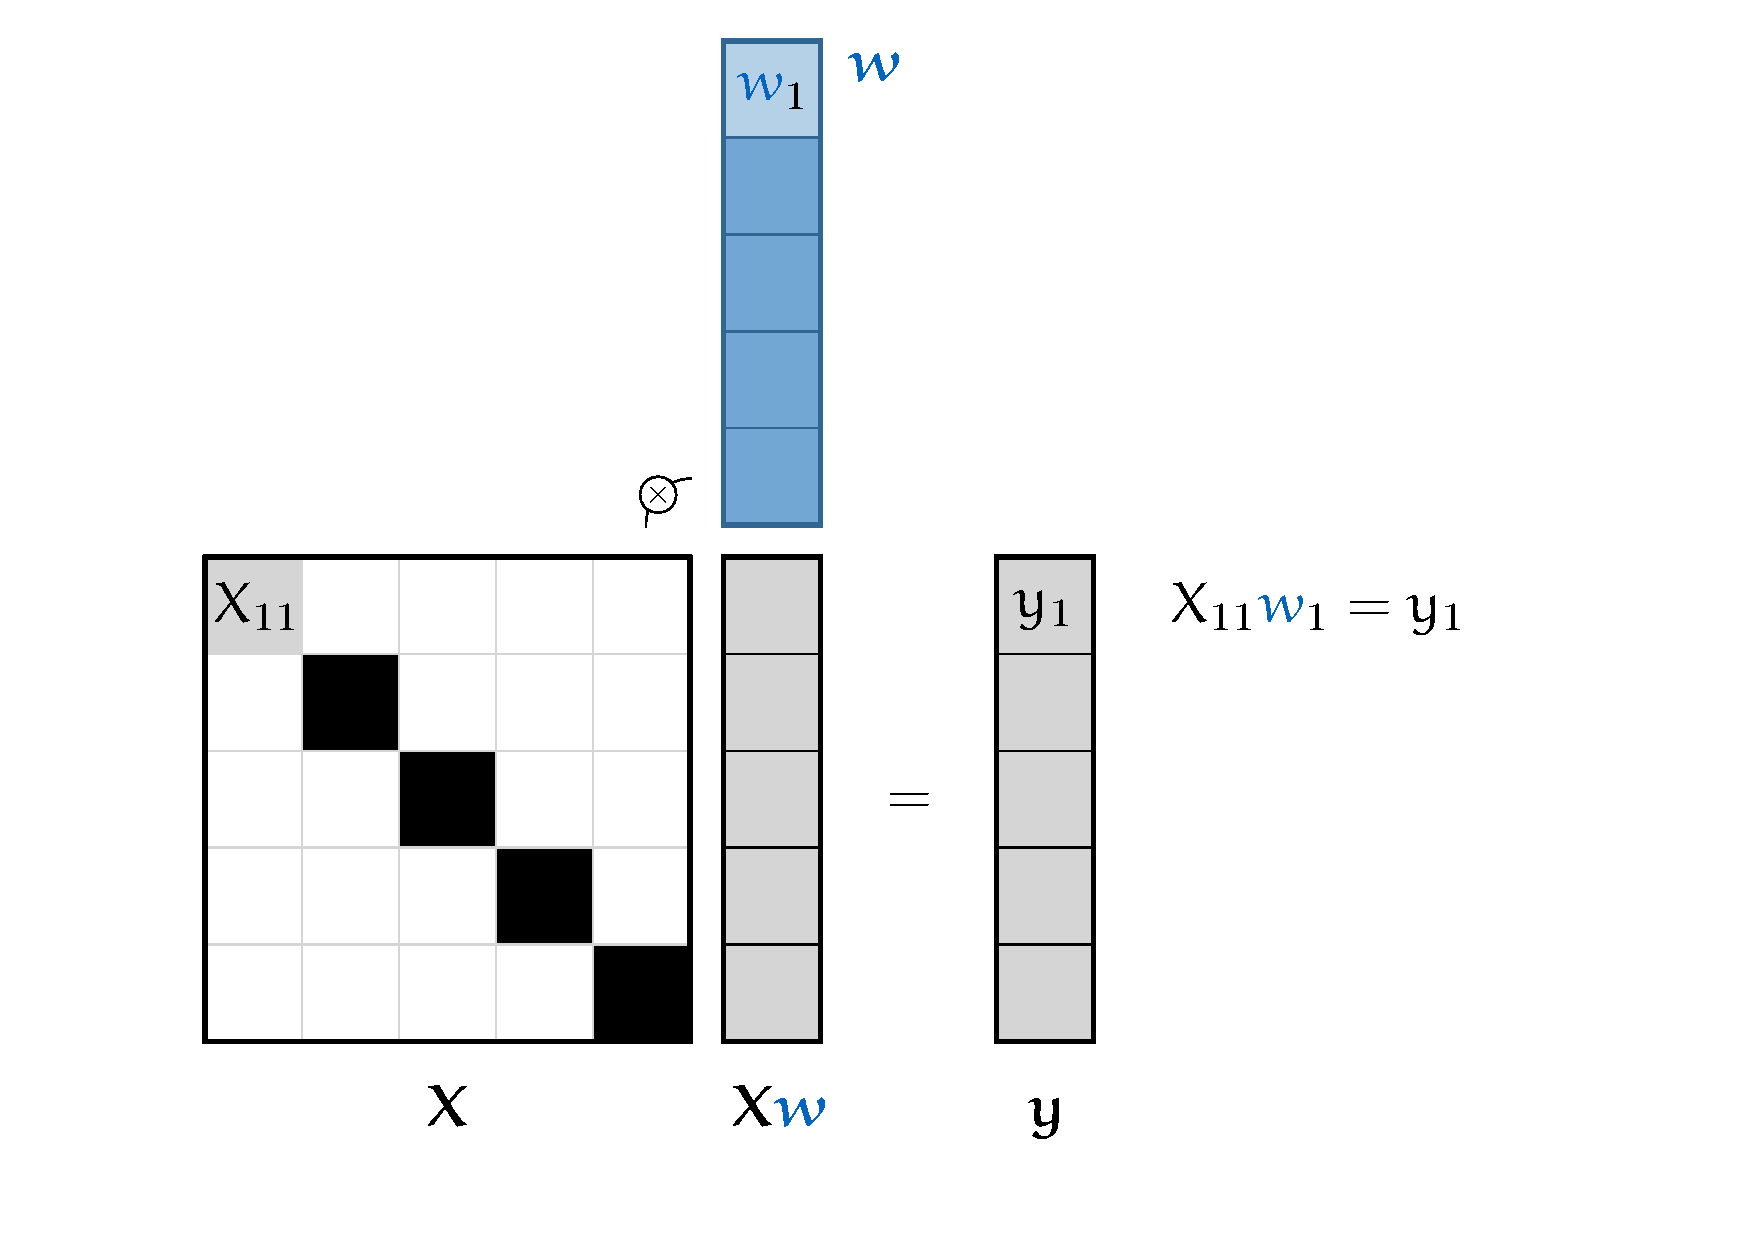
\includegraphics[width=0.7\textwidth]{./images/pca-4/diagonal.pdf}
	}
	\caption*{The very simplest setting for the problem \(\mbX\bc{\mbw} = \mby\) is when \(\mbX\) is square and diagonal. In that case, each \(\bc{w}_i\) can be solved as a simple scalar equation.
	}
\end{figure}

%<figure class="narrow centering">
%<img src="/images/pca-4/diagonal.svg" class="three-quarters">
%<figcaption>The very simplest setting for the problem \(\X\bc{\w} = \y\) is when \(\X\) is square and diagonal. In that case, each \(\bc{w}_i\) can be solved as a simple scalar equation.
%</figcaption>
%</figure>

What we see here is that for a diagonal matrix, the choices for each \(\bc{w}_i\) become in a sense \emph{independent}. The only requirement for \(\bc{w}_1\) is that it makes \(X_{11}\bc{w}_1\) as close as possible to \(y_1\). We can make them equal by setting \(\bc{w}_1 = y_1 / X_{11}\), without worrying about the other parts of \(\mbX\) or \(\bc{\mbw}\). We can do the same thing for every \(\bc{w}_{i}\).

If \(\mbX\) is not square, but it is still diagonal, we get some extra zero rows or extra zero columns. In the first case, we can't control the elements of \(\mbX\bc{\mbw}\) corresponding to the zero rows, so we may not be able to produce \(\mby\) exactly. The best solution is to optimize for the values we can control. In short, the solution in the previous paragraph will give us the orthogonal projection onto the column space of \(\mbX\). In the second case, when \(\mbX\) is wide, we get some extra elements of \(\bc{\mbw}\), which we can set to whatever we like, because they correspond to zero columns. Setting these to zero will give us the minimal-norm solution.  

\enlargethispage{4em}

\begin{figure}[H]
	\centerline{
		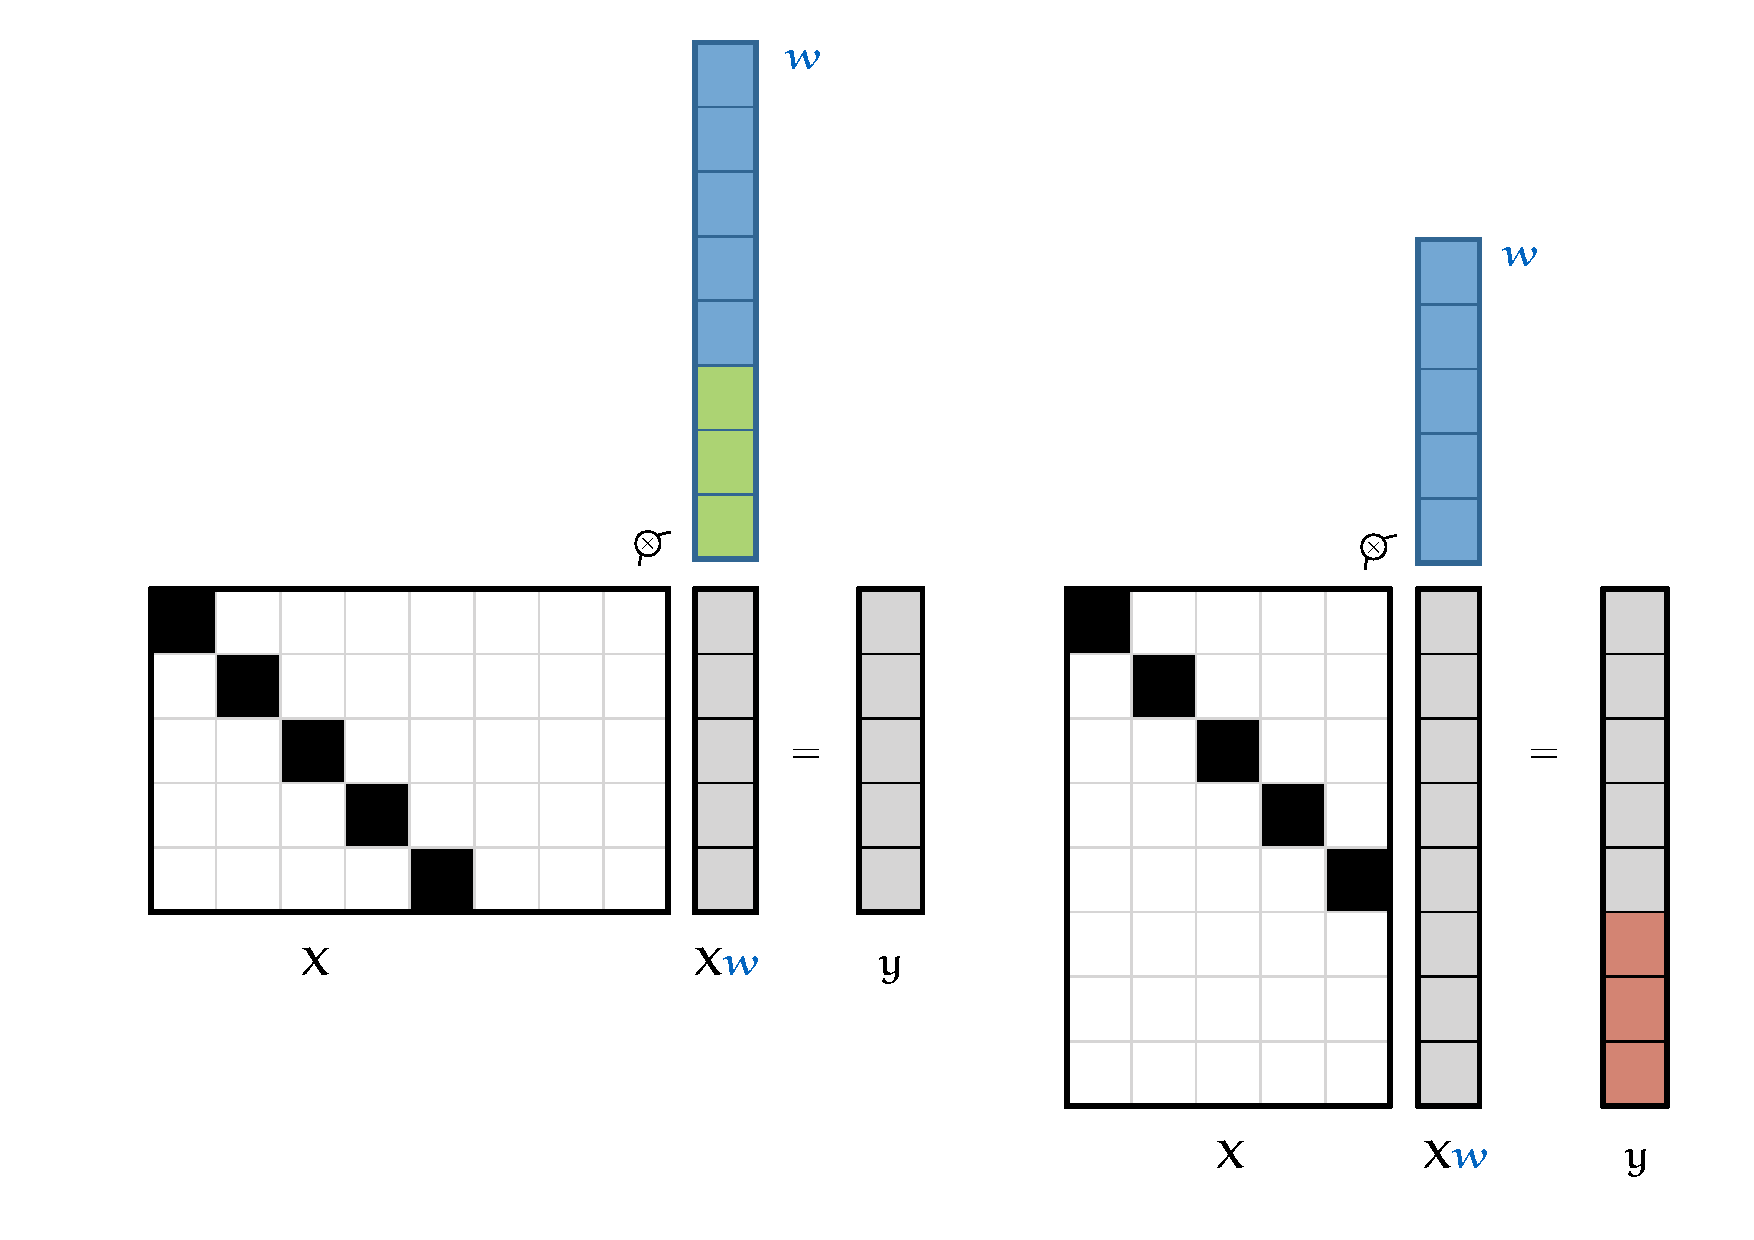
\includegraphics[width=0.8\textwidth]{./images/pca-4/diagonal-rect.pdf}
	}
	\caption*{If we have a diagonal, non-square \(\mbX\), two situations can arise. If \(\mbX\) is wide, we get \gc{some entries} in \(\bc{\mbw}\) corresponding to zero-columns. We have an underdetermined problem with multiple possible solutions. We get the solution with the smallest norm by setting these entries to zero. If we have a tall \(\mbX\), we have \rc{some entries} in \(\mby\) corresponding to zero rows. This means we can never make \(\mbX\bc{\mbw}\) exactly equal to \(\mby\). We have an overdetermined problem, and the best we can do is to minimize \(\|\mbX\bc{\mbw} - \mby\|\). We do this by ensuring that the elements of \(\mbX\bc{\mbw}\) we \emph{can} control are equal to the corresponding elements of \(\mby\).
	}
\end{figure}

%<figure class="narrow centering">
%<img src="/images/pca-4/diagonal-rect.svg">
%<figcaption>If we have a diagonal, but non-square \(\X\), two situations can arise. If \(\X\) is wide, we get <span class="gc">some entries</span> in \(\bc{\w}\) corresponding to zero-columns. We have an underdetermined problem with multiple possible solutions. We get the solution with the smallest norm by setting these entries to zero. If we have a tall \(\X\), we have <span class="rc">some entries</span> in \(\y\) corresponding to zero rows. This means we can never make \(\X\bc{\w}\) exactly equal to \(\y\). We have an overdetermined problem, and the best we can do is to minimize \(\|\X\bc{\w} - \y\|\). We do this by ensuring that the elements of \(\X\bc{\w}\) we <em>can</em> control are equal to the corresponding elements of \(\y\).
%</figcaption>
%</figure>

The important thing, in both cases, is that we can work out the optimal solution simply by solving the scalar equation \(X_{ii}\bc{w}_i = y_i\) for every \(\bc{w}_i\) individually.

When we studied eigenvectors, after we saw how easy things were for a diagonal matrix, all we needed to do to deal with non-diagonal matrices was to develop a \emph{diagonalization}: a way to transform space to a basis where the transformation expressed by our matrix \emph{becomes} expressed by a diagonal matrix.

\index{eigendecomposition}

That was the eigendecomposition. The singular value decomposition does the same thing for us here. It takes any non-diagonal matrix, and it gives us \emph{two} orthogonal basis transformations \(\rc{\mbU}\) and \(\rc{\mbV}\), one for the input space and one for the output space so that the remainder of the transformation can be expressed as a (rectangular) diagonal matrix.

We can see this happen more clearly if we rewrite directly from the minimization objective. Note first that if we take the full SVD and move the basis transformation to the other side, we get \(\rc{\mbU}^T\mbX\rc{\mbV} = \gc{\Sig}\): with two changes of basis, \(\mbX\) becomes a diagonal matrix. This suggests that if we rewrite the data \(\mbX\) and the target values \(\mby\) in the right bases, the minimization becomes a simple diagonal objective. We can work out the correct transformations with some simple rewriting:

%<!-- 
%<p>\[\begin{align*}
%\| \X\bc{\w} - \y \|^2 &= \| \rc{\U}^T\X\bc{\w} \ - \rc{\U}^T\y \|^2 & \text{orth. trf. doesn't change the norm}\\
%&=\| \rc{\U}^T\X\rc{\V}\rc{\V}^T\bc{\w} \ - \rc{\U}^T\y \|^2 & \text{because } \rc{\V}\rc{\V}^T = \I \\
%&=\| \gc{\Sig}\rc{\V}^T\bc{\w} \ - \rc{\U}^T\y \|^2 & \rc{\U}^T\X\rc{\V} = \gc{\Sig} \\
%&=\| \gc{\Sig}^T\bc{\w'} \ - \y' \|^2 & \text{with } \bc{\w}' = \rc{\V}^T\bc{\w}, \y' = \rc{\U}^T\y\\
%\end{align*}\]</p>
% -->

\begin{align*} \|\mbX\bc{\mbw} - \mby\| &= \|\rc{\mbU}\gc{\Sig}\rc{\mbV}^T\bc{\mbw} - \rc{\mbU}\rc{\mbU}^T\mby \| \\
&= \|\gc{\Sig}\rc{\mbV}^T\bc{\mbw} - \rc{\mbU}^T\mby \|  \\
&= \|\gc{\Sig}\bc{\mbw}' - \mby' \| 
\end{align*}

with \(\bc{\mbw}' = \rc{\mbV}^T\bc{\mbw}\) and \(\mby' = \rc{\mbU}^T\mby\).

And with that, we have a diagonal minimization objective. If we compute the SVD of \(\mbX\), we can transform \(\mby\) to \(\mby'\) easily. Once we find a solution for \(\bc{\mbw}'\), we can easily transform it back to the desired \(\bc{\mbw}\) by reversing the basis transformation: \(\bc{\mbw} = \rc{\mbV}\bc{\mbw}'\).

For the \(\bc{\mbw}'\) that solves the diagonal problem, there are a few different possible situations.

For now, let's stick with the assumption that \(\mbX\) is full-rank. In that case, \(\gc{\Sig}\) has non-zero elements all along its diagonal. We simply set \(\bc{w}_i'\) equal to \(y_i \gc{\Sigma}_{ii}\) and we exactly solve our problem. If \(\gc{\Sig}\) is taller than it is wide, we have some left-over values of \(\bc{\mbw}'\) with no corresponding elements of \(\gc{\Sig}\). We can set these to whatever we like, so if we want the \(\bc{\mbw}'\) with the smallest norm, we should set them to \(0\).

\begin{aside}As before, we only get a perfect solution if \(\gc{\Sig}\) is square or wide (assuming it's full rank). If it's tall, we have a bunch of rows we can't control, and we have to settle for the orthogonal projection.
\end{aside}

Now, what do we do if \(\mbX\) is rank deficient? In that case, some of the diagonal values of \(\gc{\Sig}\) will be zero. If we follow the simple definition of the pseudo-inverse, and fill in the SVD, we get stuck at:

\[\mbX^\dagger \overset{?}{=} \left( \rc{\mbV}\gc{\Sig}^2\rc{\mbV}^T \right)^{-1} \rc{\mbV}\gc{\Sig}\rc{\mbU}^T \p\]

Only the first \(k\) diagonal values of \(\gc{\Sig}^2\) are nonzero, so \(\rc{\mbV}\gc{\Sig}^2\rc{\mbV}^T\) does not have an inverse. The limit definition tells us to instead take the inverse  of \(\rc{\mbV}\gc{\Sig}^2\rc{\mbV}^T + \oc{\epsilon}\mbI\), and to let \(\oc{\epsilon}\) go to zero. Why does this lead to the algorithm we described earlier? To me, it's not immediately clear that adding these \(\oc{\epsilon}\)s will result in us ignoring the zeros on the diagonal of \(\gc{\Sig}\), which is what the algorithm tells us to do.

Luckily, it's easier to see in the minimization objective. We start with the modified normal equation

\[(\mbX^T\mbX + \oc{\epsilon}\mbI)\bc{\mbw} = \mbX^T\mby\p\]

Since \(\mbX\) is rank deficient, this doesn't have an exact solution. Instead, we can minimize the norm of the difference between the left and right sides. With a little rewriting, we get:

\begin{align*}
\| (\mbX^T\mbX + \oc{\epsilon}\mbI)\bc{\mbw} - \mbX^T\mby \| &= \| (\rc{\mbV}\gc{\Sig}^T\rc{\mbU}^T\rc{\mbU}\gc{\Sig}\rc{\mbV}^T + \oc{\epsilon}\rc{\mbV}\rc{\mbV}^T)\bc{\mbw} - \rc{\mbV}\gc{\Sig}^T\rc{\mbU}^T\mby \| \\
&= \| (\gc{\Sig}^T\gc{\Sig}\rc{\mbV}^T + \oc{\epsilon}\rc{\mbV}^T)\bc{\mbw} - \gc{\Sig}^T\rc{\mbU}^T\mby \| \\
&= \| (\gc{\Sig}^T\gc{\Sig} + \oc{\epsilon}\mbI)\rc{\mbV}^T\bc{\mbw} - \gc{\Sig}^T\rc{\mbU}^T\mby \| \\
&= \| (\gc{\Sig}^2 + \oc{\epsilon}\mbI)\bc{\mbw'} - \mby' \|
\end{align*}

where we've set \(\mby' = \gc{\Sig}^T\rc{\mbU}^T\mby\) and \(\bc{\mbw}' = \rc{\mbV}^T\bc{\mbw}\). It's a bit more complex than what we had before, but the principle is the same.

In the final line, we see that we again have a simple linear problem with a diagonal matrix: \(\gc{\Sig}^2 + \oc{\epsilon}\mbI\). 

\pagebreak\noindent The solution to this problem is to solve, for each \(\bc{w'}_i\), the scalar equation  \(({\gc{\Sigma}_{ii}}^2 + \oc{\epsilon}) \bc{w'}_i = {y'}_i\), which gives us  

\[\bc{w'}_i = \frac{ {y'}_i }{ {\gc{\Sigma}_{ii}}^2 + \oc{\epsilon} } \p\] 

From the definition of \(\mby'\), we see that \(y'_i = \gc{\Sigma}_{ii} {\rc{\mbu}_{i} }^T \mby\) where \(\rc{\mbu}_{i}\) is the \(i\)-th column of \(\rc{\mbU}\). Filling this in, we get

\[
\bc{w'}_i = \frac{\gc{\Sigma}_{ii} \kc{\;\times\;{\mbu_i} ^T\mby}}{{\gc{\Sigma}_{ii}}^2 + \oc{\epsilon}} \p
\]

Here, we can see clearly where the problem of invertibility occurs: if \(\gc{\Sigma}_{ii}\) is zero, and we don't add \(\oc{\epsilon}\), we get a division by zero, which is undefined. The small \(\oc{\epsilon}\) added to the diagonal of \(\mbX^T\mbX\) ends up being added to the denominator, so we are preventing this division by zero.

\begin{aside}Since \(\gc{\Sig}_{ii}\) also occurs in the numerator, we know that these divisions by zero will always be instances of \(0/0\). The addition of \(\oc{\epsilon}\) in the denominator turns this value into \(0\).	
\end{aside}

The addition of \(\oc{\epsilon}\) also affects the result for \(\bc{w'}_i\) where \(\gc{\Sig}_{ii}\) is nonzero, but we eliminate this effect by letting \(\oc{\epsilon}\) go to zero. In that case, the solution goes to \(\bc{w}_i = {\gc{\Sigma}_{ii}}^{-1} {\rc{\mbu}_i} ^T\mby\)

Putting all this together, we can derive the algorithm we already know. Given \(\mbX\), we compute its SVD \(\rc{\mbU}\gc{\Sig}\rc{\mbV}^T\). We transform our targets \(\mby\) to a new basis \(\mby' = \gc{\Sig}^T\rc{\mbU}^T\mby\). We solve the diagonal problem 

\[\argmin{\bc{\mbw'}}\;\left \| \left( \gc{\Sig}^2 + \oc{\epsilon}\mbI \right)\bc{\mbw'} - \mby'\right\| \]

which we've shown above gives us 

\[\bc{w}'_i = {\gc{\Sigma}_{ii}}^{-1} y_i' = {\gc{\Sigma}_{ii}}^{-1} {\rc{\mbu}_i}^T\mby \]

if \(\gc{\Sigma}_{ii} \neq 0\) and \(\bc{w}'_i = 0\) otherwise. In matrix notation, we can write 

\[\bc{\mbw'} = \gc{\Sig}^\dagger\rc{\mbU}^T\mby \p\]

\pagebreak\noindent Finally, we translate \(\bc{\mbw'}\) back to \(\bc{\mbw}\) by multiplying by \(\bc{\mbV}\):

\[\bc{\mbw} = \rc{\mbV}\bc{\mbw'} = \rc{\mbV}\gc{\Sig}^\dagger\rc{\mbU}^T\mby = \mbX^\dagger\mby\]

which is the algorithm we started out with.

As always, there are other ways of computing the pseudo-inverse, but we like the SVD method, because we can very cleanly eliminate any noise by simply taking the singular values that are close to zero and treating them as zero.

So, what have we learned? Firstly, that the least squares linear regression problem is solved by forming the pseudo-inverse, and secondly, that the pseudo-inverse can be computed very robustly by taking the SVD, inverting the nonzero values of \(\gc{\Sig}\), multiplying it back together and transposing it.

But don't think that all this is good for is linear regression. What we've shown here is the basis behind pretty much any linear learning method. Imagine that you have a large space of points \(\mR^n\) and some target \(\mby\) anywhere in that space. You are looking for a point \(\mbx \in \mR^n\) as close to \(\mby\) as possible but under the constraint that \(\mbx\) is in some linear subspace \(\rc{P}\) of dimension \(n\). In that case the pseudo-inverse will give you your solution, quickly and precisely. This may sound a bit abstract, but it covers a huge swathe of search problems in machine learning, optimization and computer vision.

Even if your problem isn't linear, for instance if you're training a neural network, this can be a worthwhile perspective. Such models are usually trained by assuming that they are \emph{locally} linear, computing the linear solution to this local approximation, and then taking a small step towards this solution. This is, for instance, how gradient descent operates. Even if you are training a non-linear model, the linear perspective can tell you a lot.

\enlargethispage{1em}

Finally, it's worth taking a minute to consider what all this boils down to. The best approximation theorem at heart is nothing more than an application of the Pythagorean theorem. When I first learned that theorem, long ago, I didn't really get what the big deal was, why this theorem was so much more famous than any other one in Euclidean geometry. Now, I see that pretty much everything we do in statistics and machine learning comes down to the best approximation theorem, which in turn is built on the Pythagorean theorem.

\section{Making use of the SVD}

To finish up, let's see what else the pseudo-inverse and SVD can do for us. I promised that the basic framework of the best approximation theorem popped up in a lot of places, so let's make good on that promise with a few examples. The last example will, once again, bring us back to principal component analysis.

\subsection{Compression and noise removal}

Let's start by looking a little closer at something we've glossed over in the story so far: the idea of \emph{noise}. We've said that one of the main benefits of the SVD is that it easily allows us to remove noise. If we have a low-rank matrix that contains some data that we're interested in, but through some process like measurement error or floating point computation, a little noise has been added, we saw that the singular values that were zero before will now be small non-zero values. Setting these back to zero removes a large part of the noise.

\index{Noise}

The idea of noise is an important and very deep subject in machine learning and statistics. If you look up an official definition of noise in data analysis, you may find some assertion that the noise is the ``random part'' of the data. The pattern is caused by a mechanism, and the noise is a random signal ``without cause'' that is added on top. The pattern and the noise together make the data we observe.

This is an interesting perspective, but in practice it doesn't quite work like that. What constitutes noise is usually a \emph{subjective} choice. Two people may look at the same data, and consider different parts noise. To explain, imagine that you've decided to weigh yourself regularly and to analyse the resulting data. 

If you're looking to lose weight, you're probably only interested in a rough weekly trend. The daily fluctuations won't mean much, but over a whole week, you can tell whether your current diet and exercise regime is working. In this view, the first-order trend  is all you're interested in. The rest you can treat as random noise. It's not random in the sense that there is no cause behind it, it's just that we are interested in looking at the data at a more granular level.

If you are interested in something else, you may want to retain more of the data. For instance, you might wonder whether it's true that eating starchy food causes you to retain water, increasing your weight the next day. In that case, you are interested in the difference between successive days, based on what you ate the day before. You may even be interested in the way in which your metabolism changes throughout the day, in which case, you'd want to retain all the fine detail of the data over the course of the day (assuming you weigh yourself often enough).

In short, what you consider noise and what you consider pattern is a subjective choice, depending on what you do want to do with the data.

In some sense this is true of almost anything we call random. In theory, we could predict quite accurately how a flipped coin will land if we had a good idea of the state of the atmosphere around the coin, and the amount of force impacting the coin at the start of the flip. In practice, we usually treat all of this as unknown: we call it noise or randomness, and we say that the coin will land either side with equal probability. It's not random because there's no cause and effect, it's random because we don't care about that part of the process.

\begin{aside}In machine learning, this problem manifests as over- and underfitting. Overfitting is when we model too much of the noise as pattern and we end up remembering parts of the data that we should be ignoring. Underfitting is when we ignore too much of the noise and apply too simple a model to the data. In machine learning, the test set is the ultimate arbiter of what we should consider pattern and what we should consider noise.	
\end{aside}

All this is just to make the point that what we filter out as noise is mostly determined by how we want to model the world. If we're interested in losing weight, we will treat the data as roughly linear (on the scale of a week), and ignore any finer detail. We will treat this as random noise when we fit a line through our data, not because it's truly random, but because the causes are too complex to model, and because they are irrelevant to our goal.

The relevance to SVD is that when we set the noise threshold in SVD, we are implicitly making this choice. So far we've said that there will be an obvious difference between the true singular vectors and those caused by noise, and often this is true, but it would be more accurate to say that we are \emph{choosing} which parts to treat as noise. 

If we wanted to, we could ramp up the threshold, and also zero out some of the more substantial singular vectors. The ones that were definitely not introduced by simple measurement error or floating point computations. This is essentially what happens when we compute a truncated SVD. We can either choose the number of singular vectors to retain, or set the noise threshold.

We've seen an example of this already, although we didn't know it at the time. In Chapter~\ref{chapter:introduction}, we reconstructed our face data step by step, by adding more principal components. The principal component are the singular vectors, so this process is equivalent to taking an SVD decomposition, truncated at \(k\), and looking at the reconstructed data.

\begin{figure}[H]
	\centerline{
		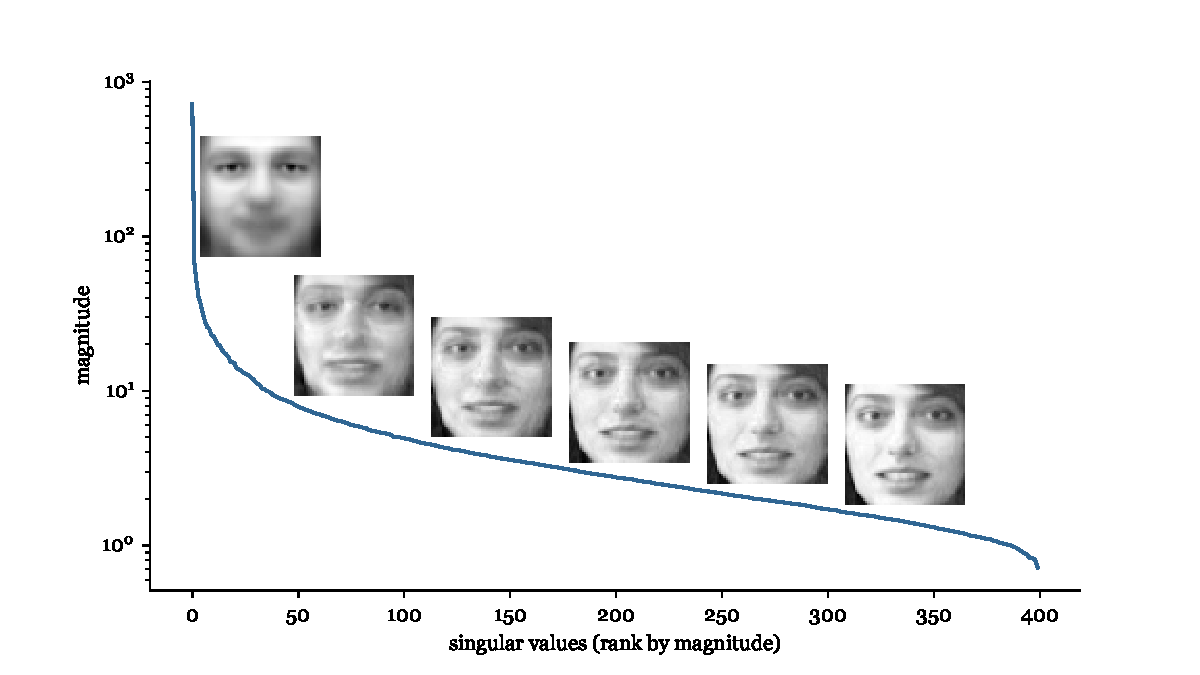
\includegraphics[width=1.1\textwidth]{./images/pca-4/faces-svs.pdf}
	}
	\caption*{A plot of the singular values of the Olivetti faces data, in order of magnitude. The insets show the reconstructions using 10, 75, 140, 205, 270 and 335 singular values and vectors.
	}
\end{figure}

%<figure class="narrow centering">
%<img src="/images/pca-4/faces-svs.svg" >
%<figcaption>A plot of the singular values of the Olivetti faces data, in order of magnitude. The insets show the reconstructions using 10, 75, 140, 205, 270 and 335 singular values and vectors.
%</figcaption>
%</figure>

We see that at the high end, we get singular values with a magnitude between \(0.1\) and \(1.0\). This corresponds to things like camera noise, compression artifacts and floating point errors in the computation of the SVD itself. Reconstructing the data from only the principal components with singular values above this noise level results in a barely noticeable smoothing of the images but little loss in identifiability.

If we set the noise threshold higher, around \(10\), we begin to lose some of the detailed facial features but the basic identity of each person is still retained. If we go even higher than that, to around \(100\), only a handful of principal components remain. We see that the faces are so smoothed out that only basic properties like gender, age and lighting direction are retained.

\begin{aside}There may not be many use cases for reconstructing the data from this few components, but there are certainly use cases for analysing the data where we may care about a subject's gender and age without caring much about what their exact face looks like.	
\end{aside}

\subsection{Compressing single images}

Representing images with their principal components in a larger dataset is a kind of image compression ``in context''. We can work out that age and gender are important attributes because they are important causes of variation in the images in the set. In practice, however, image compression happens on one image at a time, without explicit reference to a larger set of images they belong too.

In this setting, we can also apply the SVD. Instead of flattening the image into a vector, we keep the image as a grid of pixels, and treat that grid as out matrix \(\gc{\mbM}\). We'll assume we have a grayscale image with pixel values encoded as numbers between \(0\) (for black) and \(1\) (for white). What can we expect to happen if we apply an SVD to this matrix?

\[
\gc{\mbM} = \rc{\mbU}\gc{\Sig}\rc{\mbV}^T
\]

The first thing to note is that we get a perfect reconstruction (at least in theory) if we compute a full SVD. But then the three matrices \(\rc{\mbU}\), \(\gc{\Sig}\), \(\rc{\mbV}\) contain many more values than the matrix \(\gc{\mbM}\), so we're not exactly achieving compression.

%\begin{aside}What if we're storing \(\rc{\mbU}\), \(\gc{\Sig}\), \(\rc{\mbV}\) more efficiently? An orthogonal \(k \times k\)  matrix can be stored in a sequence of \(\frac{k^2 - k}{2}\) angles. This means that we can store the SVD of an \(n \times m\) matrix in \(\frac{n^2-n}{2} + \frac{m^2 - m}{2} + \text{min}(n, m)\) values, while the full matrix takes \(mn\) values to store. For a square matrix, these result in the same number of values. For a rectangular matrix, the SVD always requires more, even if we store it efficiently like this.	
%\end{aside}

What happens if we use a compact SVD? That way we still have all the information, but we don't use as many numbers to represent \(\gc{\mbM}\) as the full SVD does. In his case, it depends on the image. For some images, the whole thing may be described with only a handful of singular vectors and values. In that case, the compact SVD will be much more efficient. This happens if the image itself is a low-rank matrix.

In most cases, if we want compression, we'll need to use a \emph{truncated} SVD. That is, we will throw away information, but we will hopefully end up with an image that still looks to us like the original.

As we illustrate what this looks like, we can also show a link to the rank decomposition, we introduced earlier. This is a decomposition of the \(n \times m\) matrix \(\gc{\mbM}\) into the product \(\bc{\mbA}\rc{\mbB}\) of an \(n \times k\) matrix \(\bc{\mbA}\) and a \(k \times m\) matrix \(\rc{\mbB}\).

\enlargethispage{2em}

\begin{figure}[H]
	\centerline{
		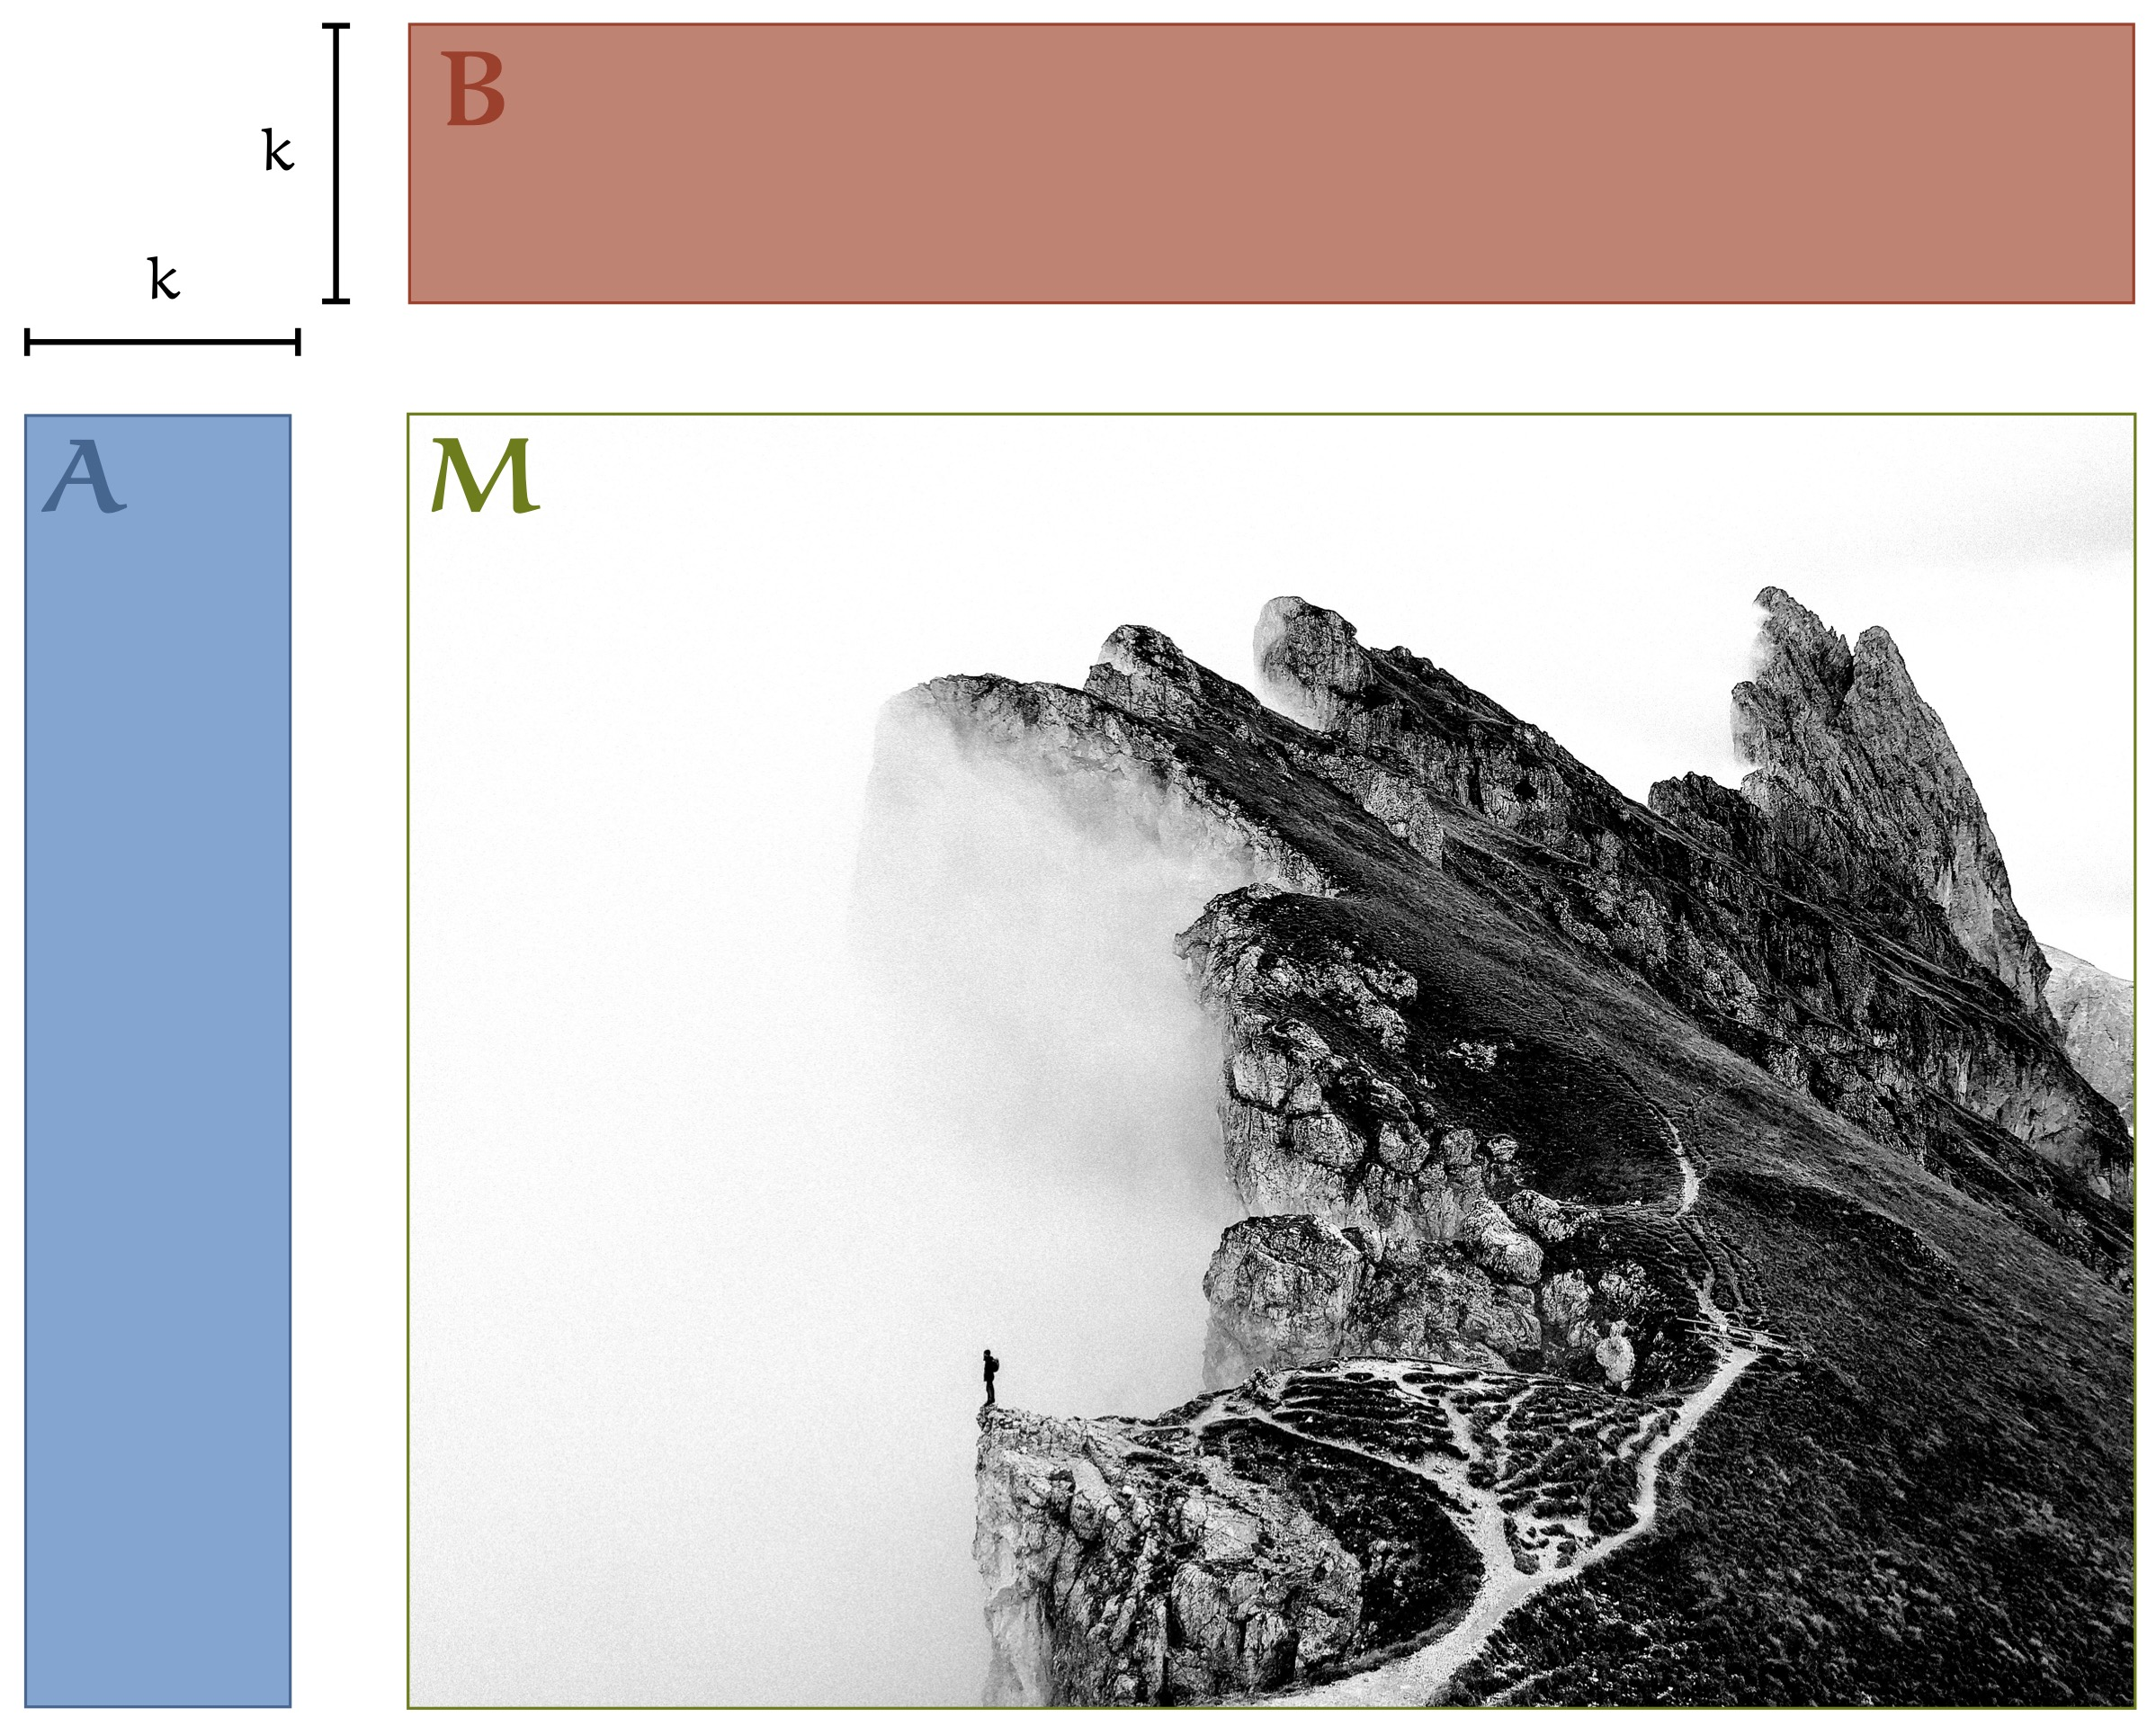
\includegraphics[width=1\textwidth]{./images/pca-4/image-rd.jpg}
	}
	\caption*{Taking a grayscale photograph, and interpreting it as a matrix, we can find a compression by applying a rank decomposition. \href{https://www.pexels.com/photo/photo-of-person-standing-on-cliff-edge-3181458}{Photograph by Tom Verdoot}.
	}
\end{figure}

%<figure class="narrow centering">
%<img src="/images/pca-4/image-rd.jpg" >
%<figcaption>Taking a grayscale photograph, and interpreting it as a matrix, we can find a compression by applying a rank decomposition. <a href="https://www.pexels.com/photo/photo-of-person-standing-on-cliff-edge-3181458/">Photograph by Tom Verdoot</a>.
%</figcaption>
%</figure>

There are plenty of interesting patterns in the above photograph, but we can also tell immediately that the matrix \(\gc{\mbM}\) is either low-rank or very close to it. On the left there are several columns of pixels that are almost entirely white, save for a gentle gradient into light gray. If just one of these columns is an exact scalar multiple of another, or a linear combination of several others, the matrix is rank deficient. More generally, because these columns are all close to being the same, we can treat them as such to compress them.

Now, how do we find the rank decomposition? It may not surprise you to learn that the SVD can help us here.

If we can find two matrices such that they multiply to form something close to \(\gc{\mbM}\), and we can keep \(k\) small enough, we will have achieved compression. We can easily turn the truncated SVD into an approximate rank decomposition: the matrices \(\rc{\mbU}_k\) and \({\rc{\mbV}_k}^T\) have the right dimensions already. All we need to do is add the singular values. The simplest thing to do is to take the squares of the  first \(k\) singular values, arrange the in a diagonal matrix \(\gc{\Sig}^\frac{1}{2}\), so that \(\gc{\Sig}^\frac{1}{2}\gc{\Sig}^\frac{1}{2} = \gc{\Sig}_k\) and write

\[\gc{\mbM} \approx \bc{\mbA}\rc{\mbB} = \rc{\mbU}_k\gc{\Sig}^\frac{1}{2}\gc{\Sig}^\frac{1}{2}\rc{\mbV}_k^T = \rc{\mbU}_k\gc{\Sig}_k\rc{\mbV}_k^T\]

with \(\bc{\mbA} = \rc{\mbU}\gc{\Sig}^\frac{1}{2}\) and \(\rc{\mbB} = \gc{\Sig}^\frac{1}{2}\rc{\mbV}^T\).

This gives us a quick way to compute a decomposition of an image matrix. Here's what this looks like at different levels of truncation.

\begin{figure}[p]

	\parbox[b]{.5\textwidth}{
		
\includegraphics[width=0.5\textwidth]{./images/pca-4/photo-cliff-001.jpeg}
	}\parbox[b]{.5\textwidth}{
		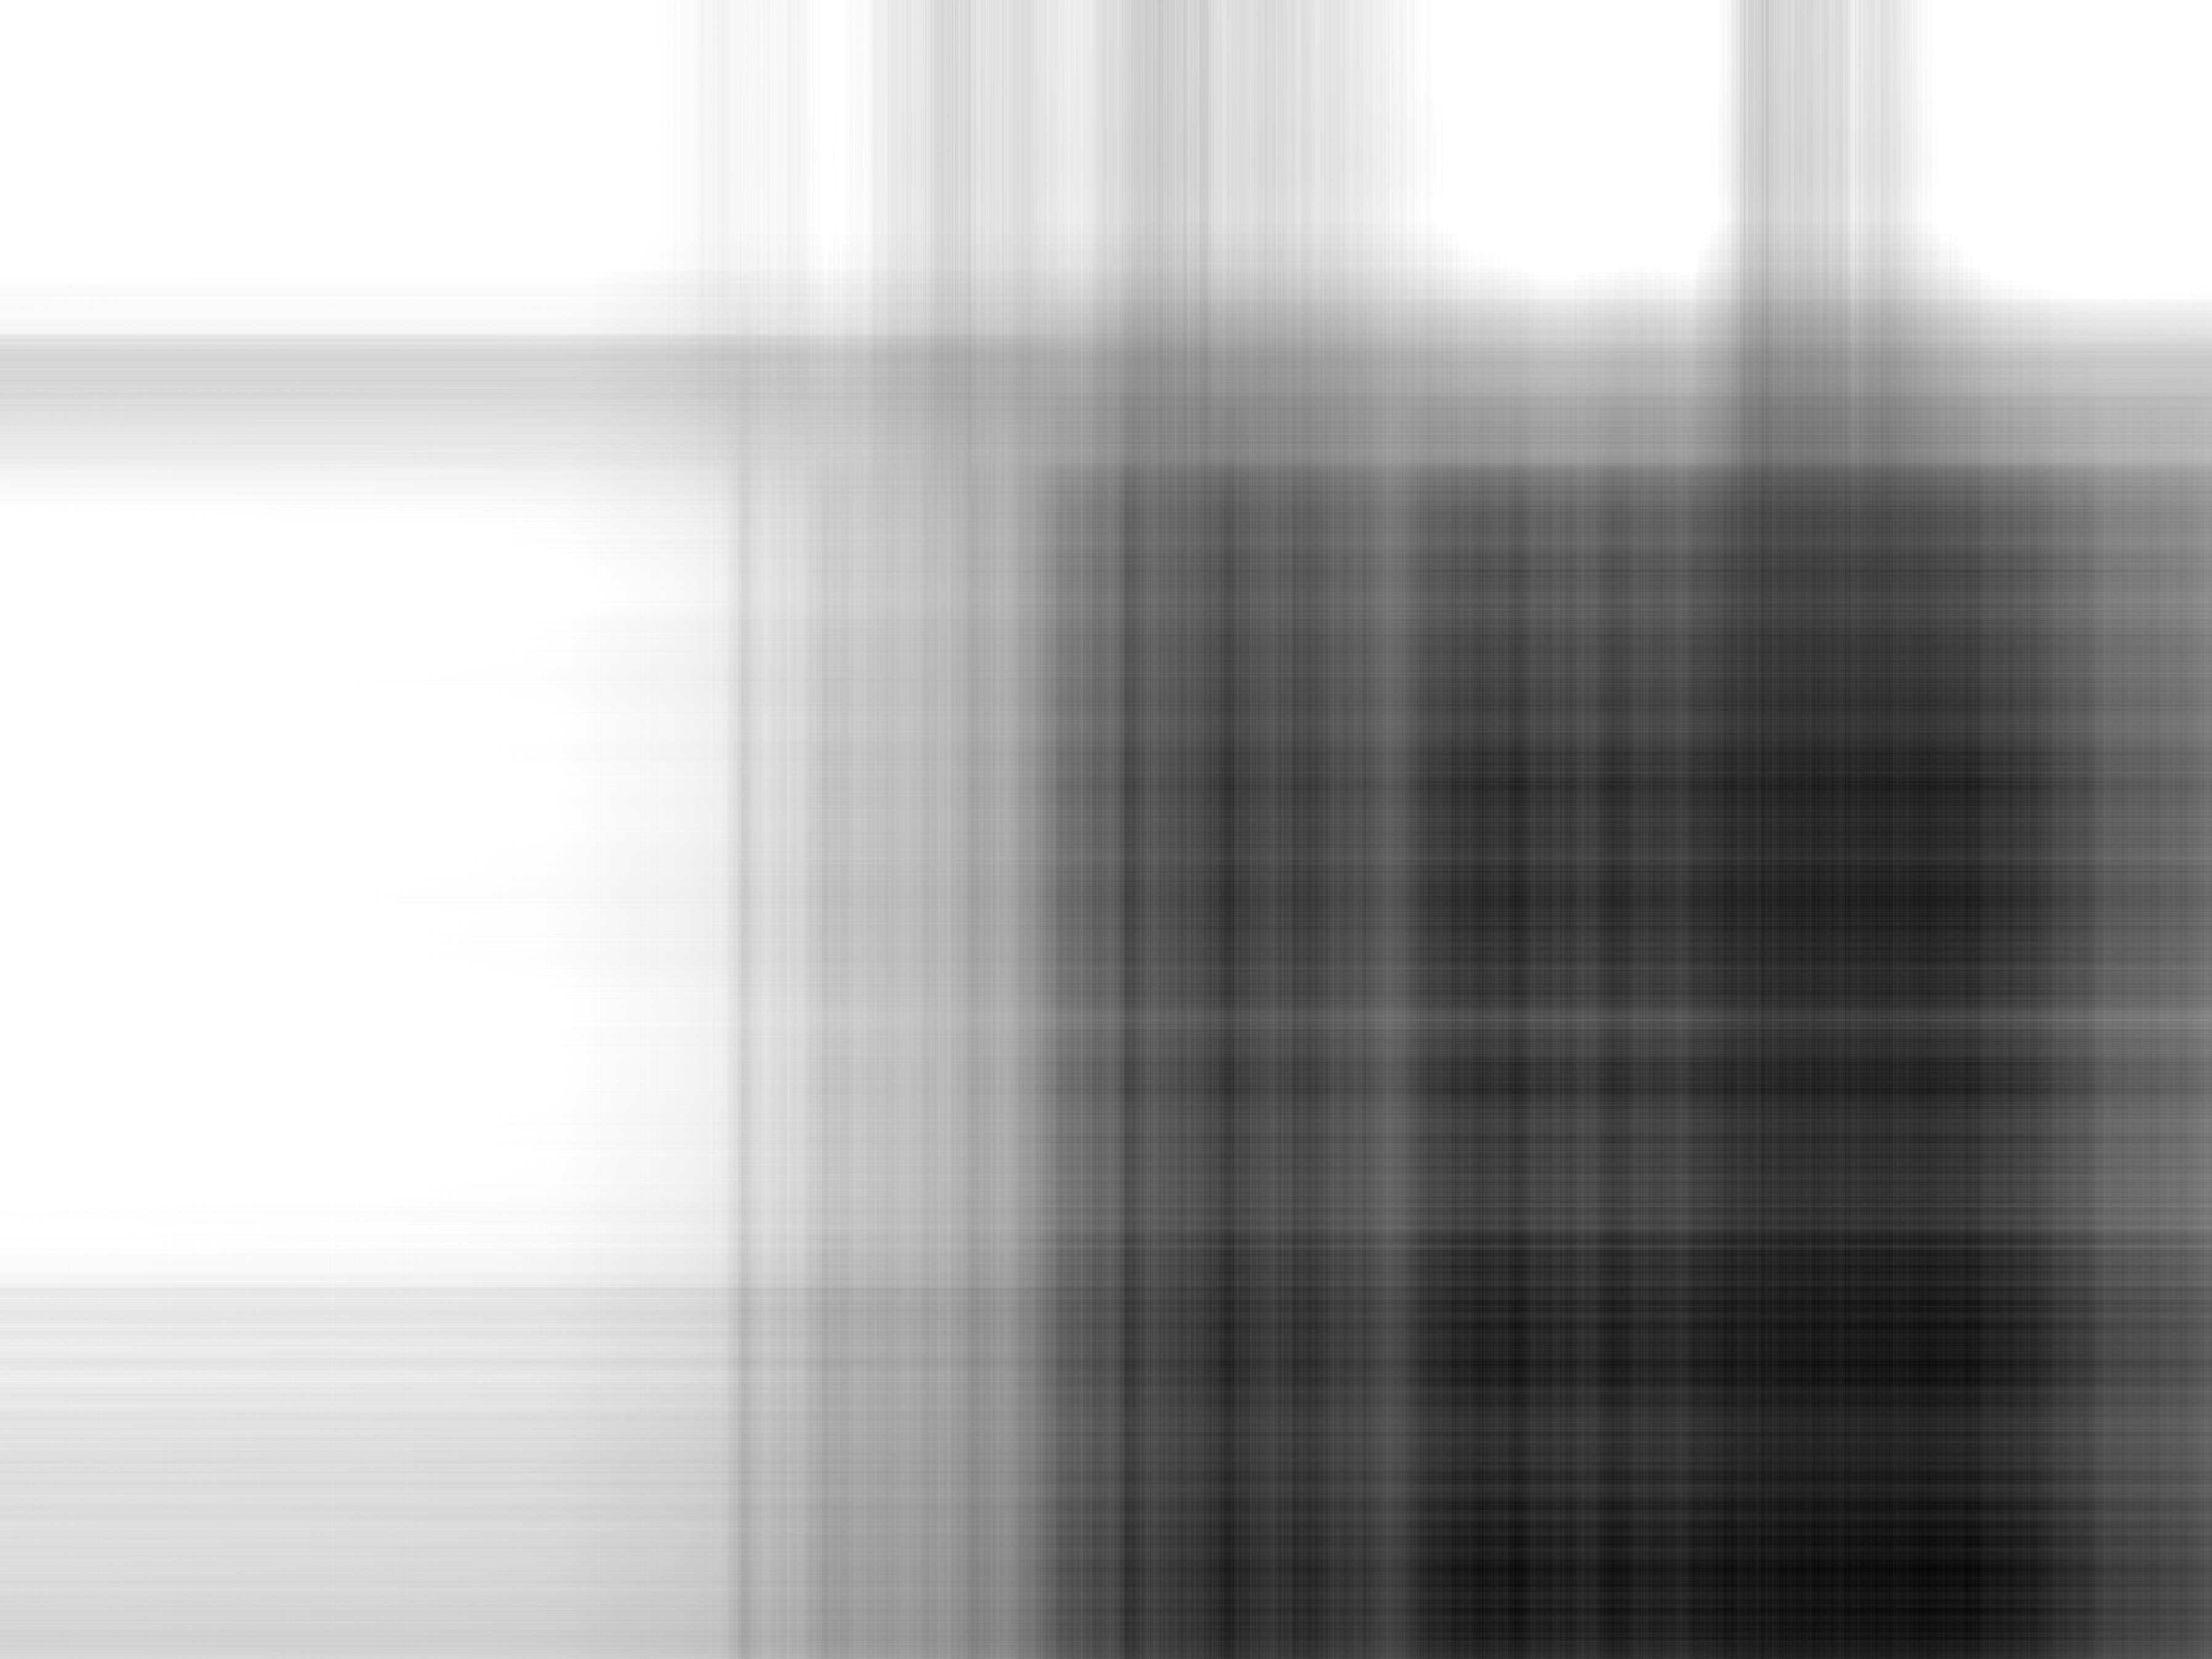
\includegraphics[width=0.5\textwidth]{./images/pca-4/photo-cliff-002.jpeg}
	}
	
	\parbox[b]{.5\textwidth}{	
		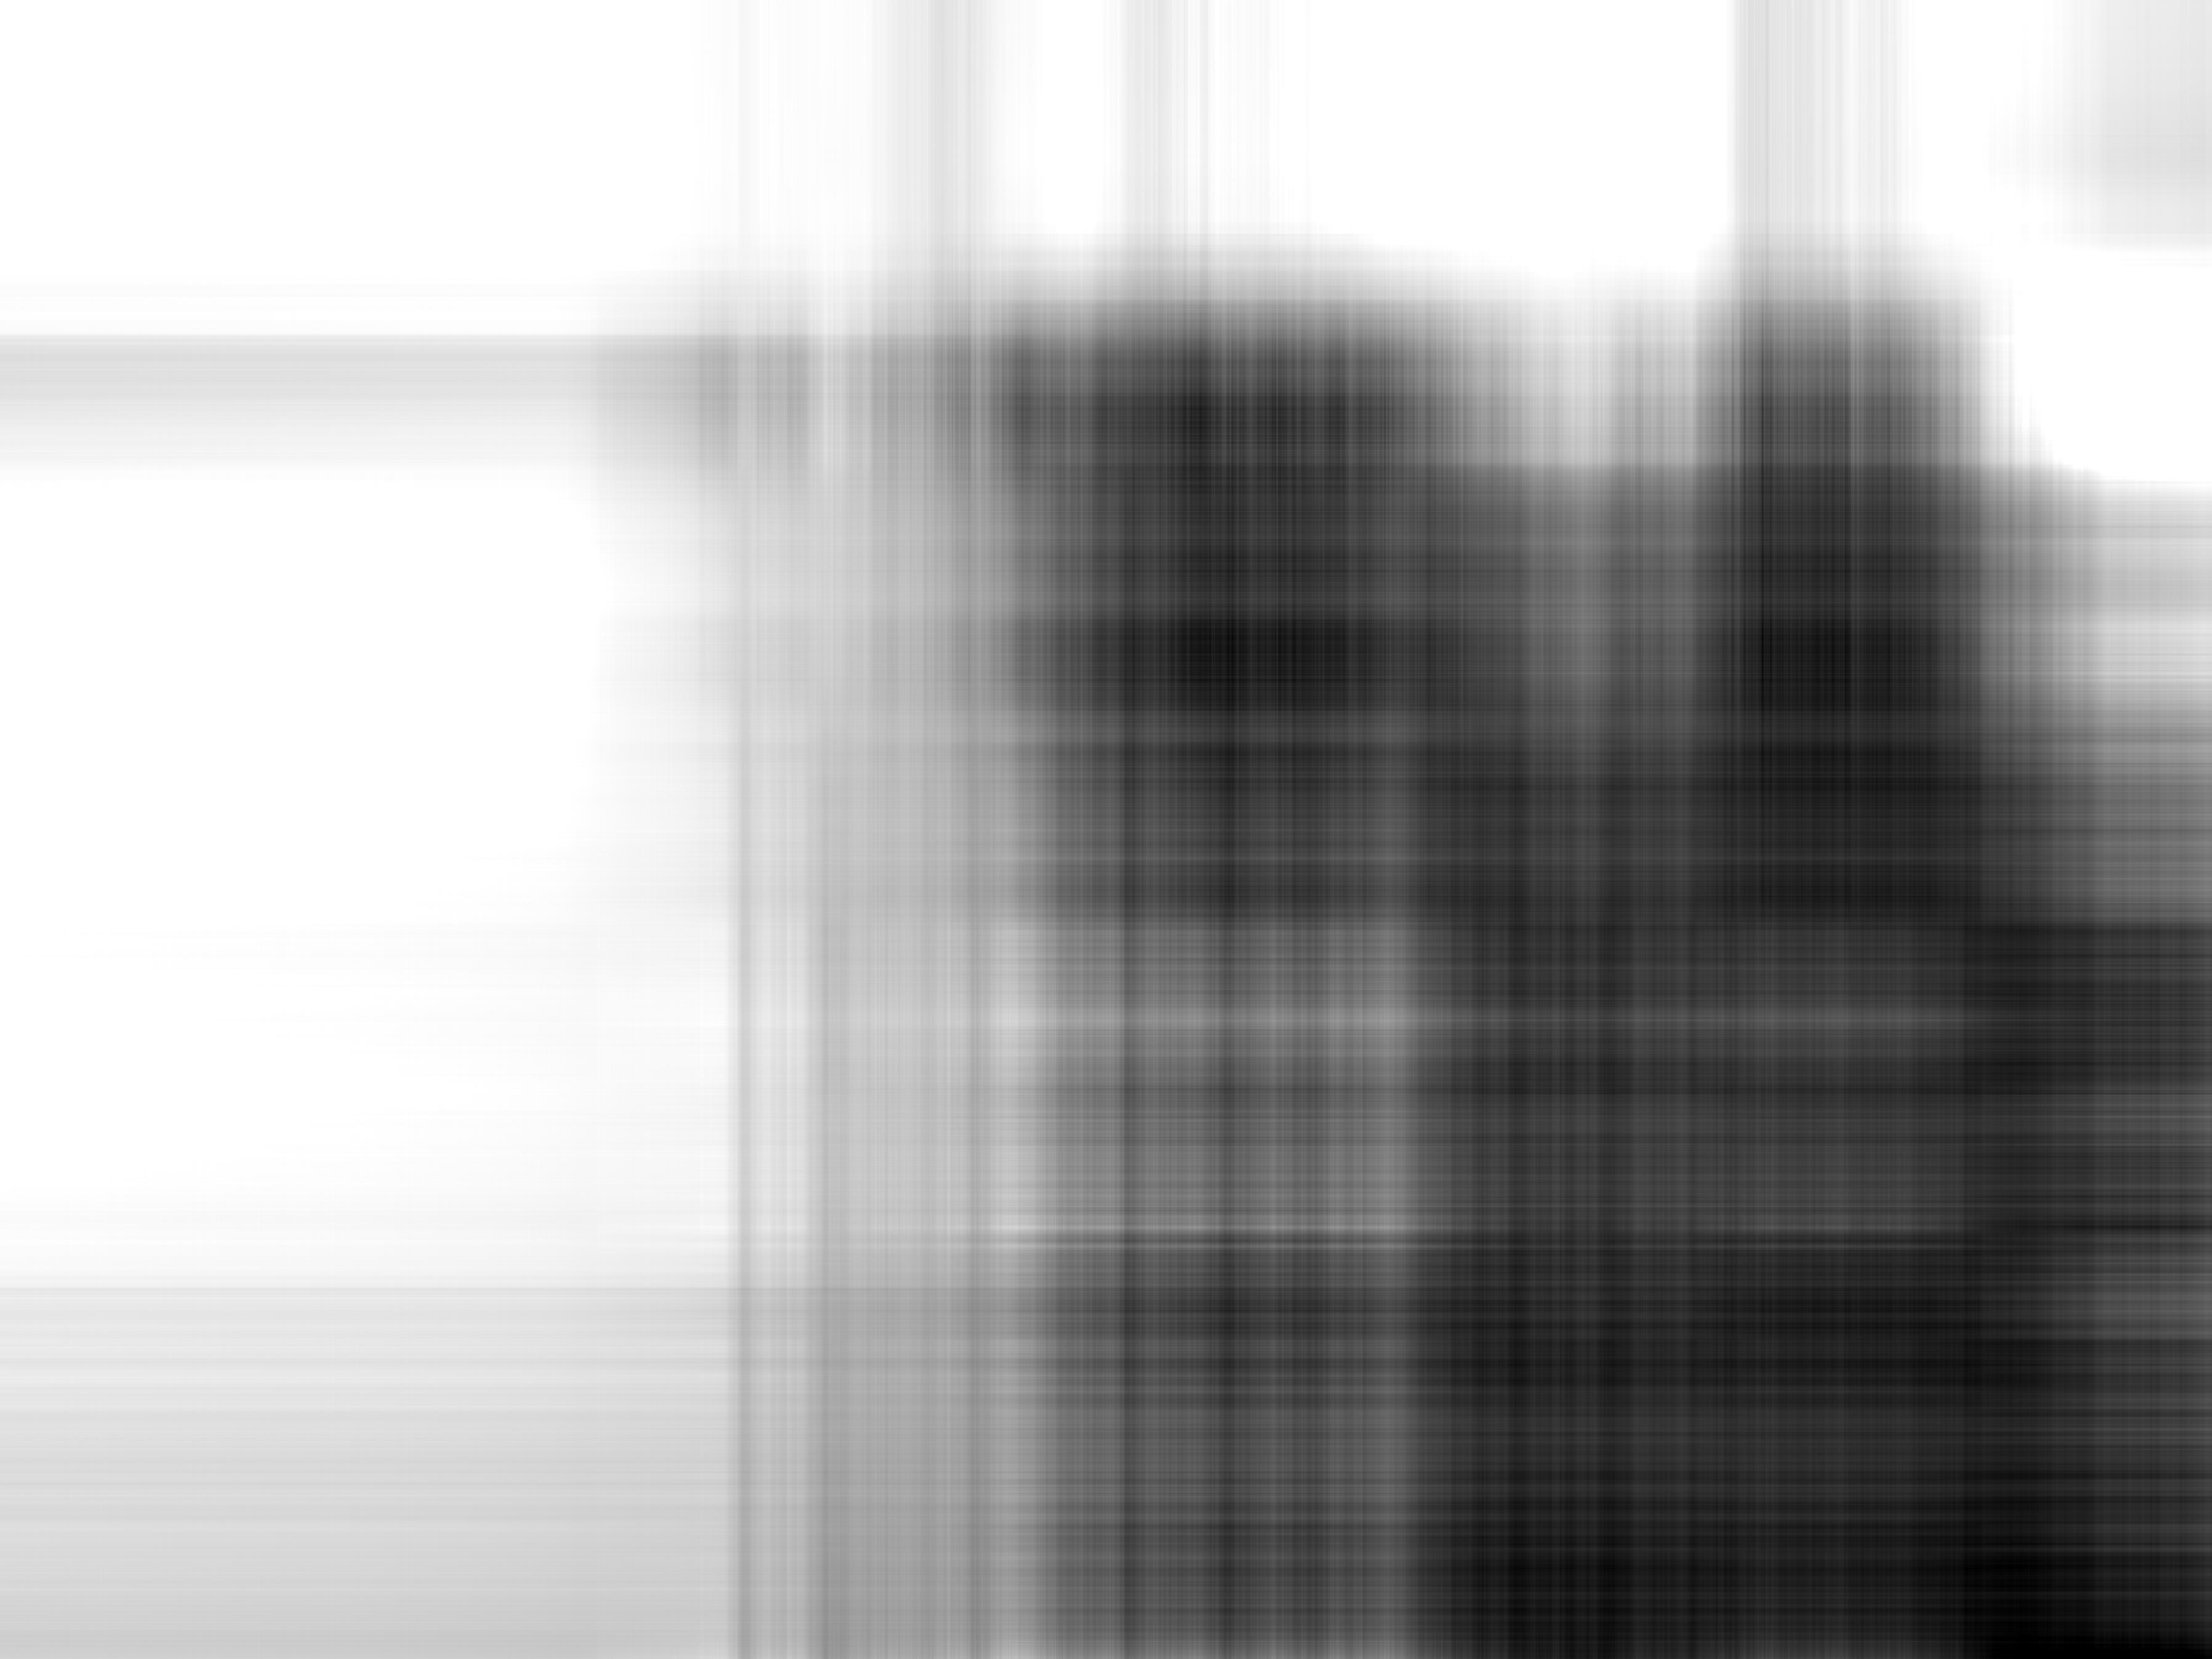
\includegraphics[width=0.5\textwidth]{./images/pca-4/photo-cliff-003.jpeg}
	}\parbox[b]{.5\textwidth}{		
		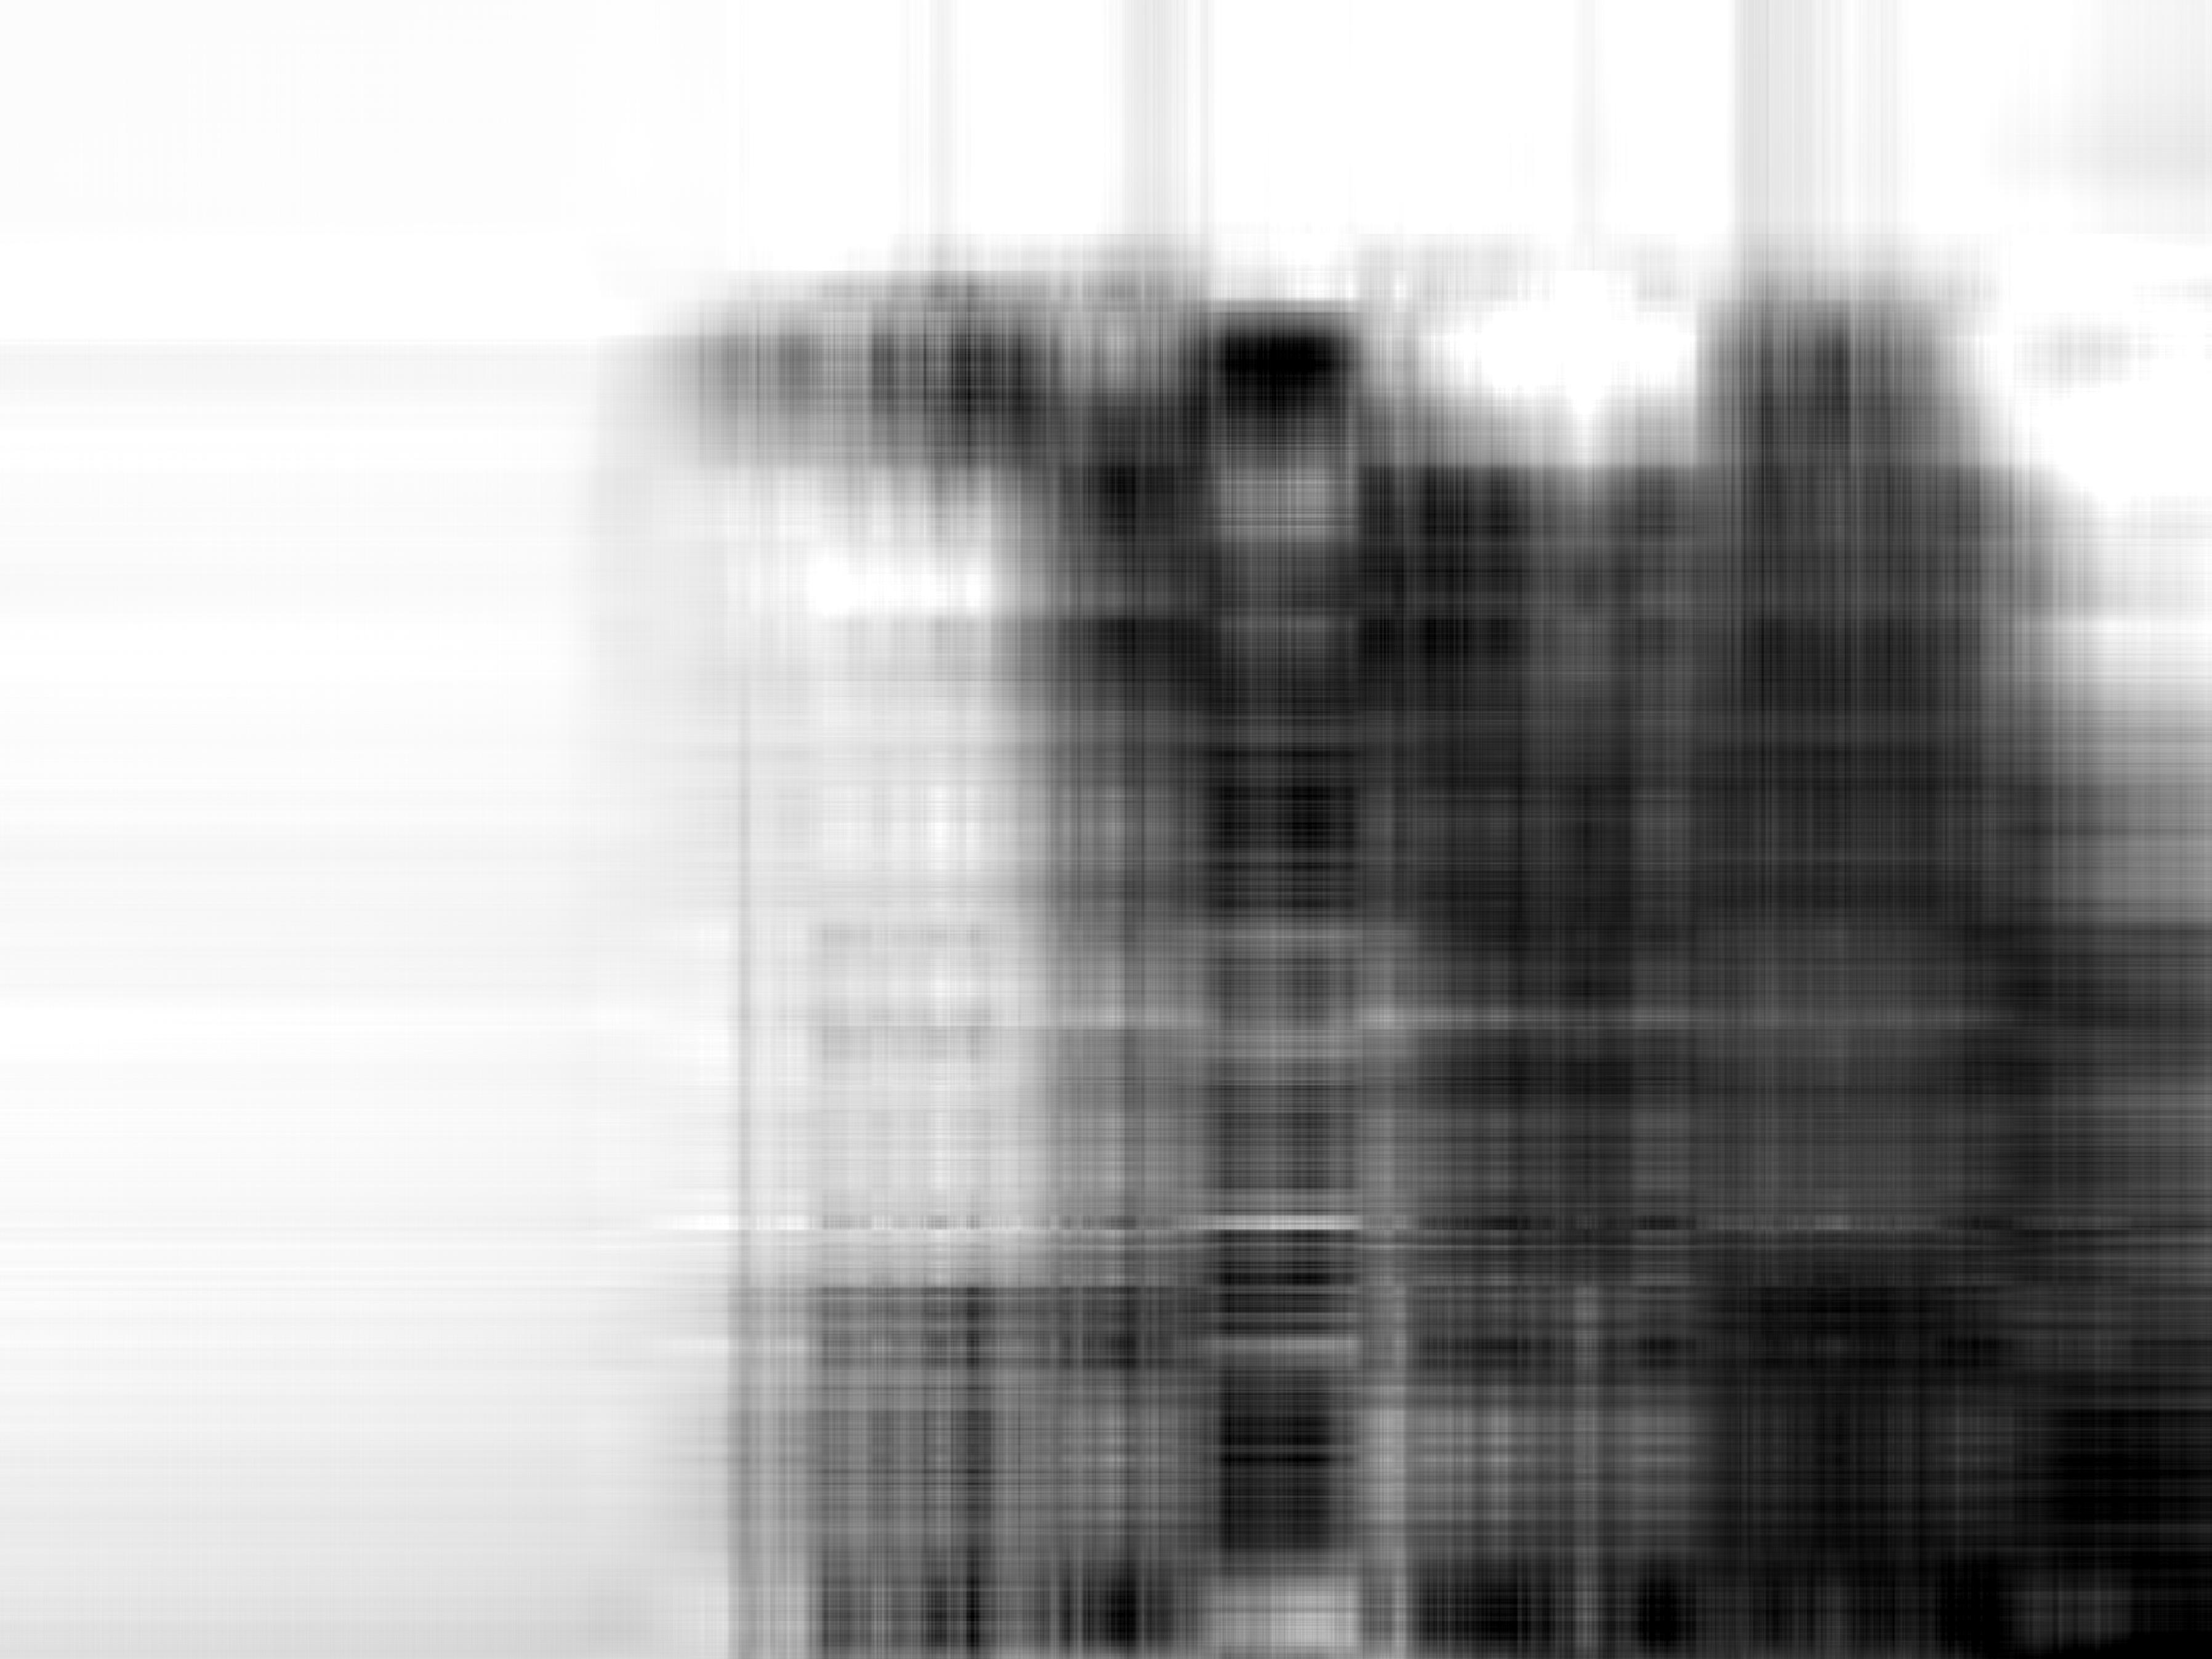
\includegraphics[width=0.5\textwidth]{./images/pca-4/photo-cliff-005.jpeg}
	}
	
	\parbox[b]{.5\textwidth}{	
		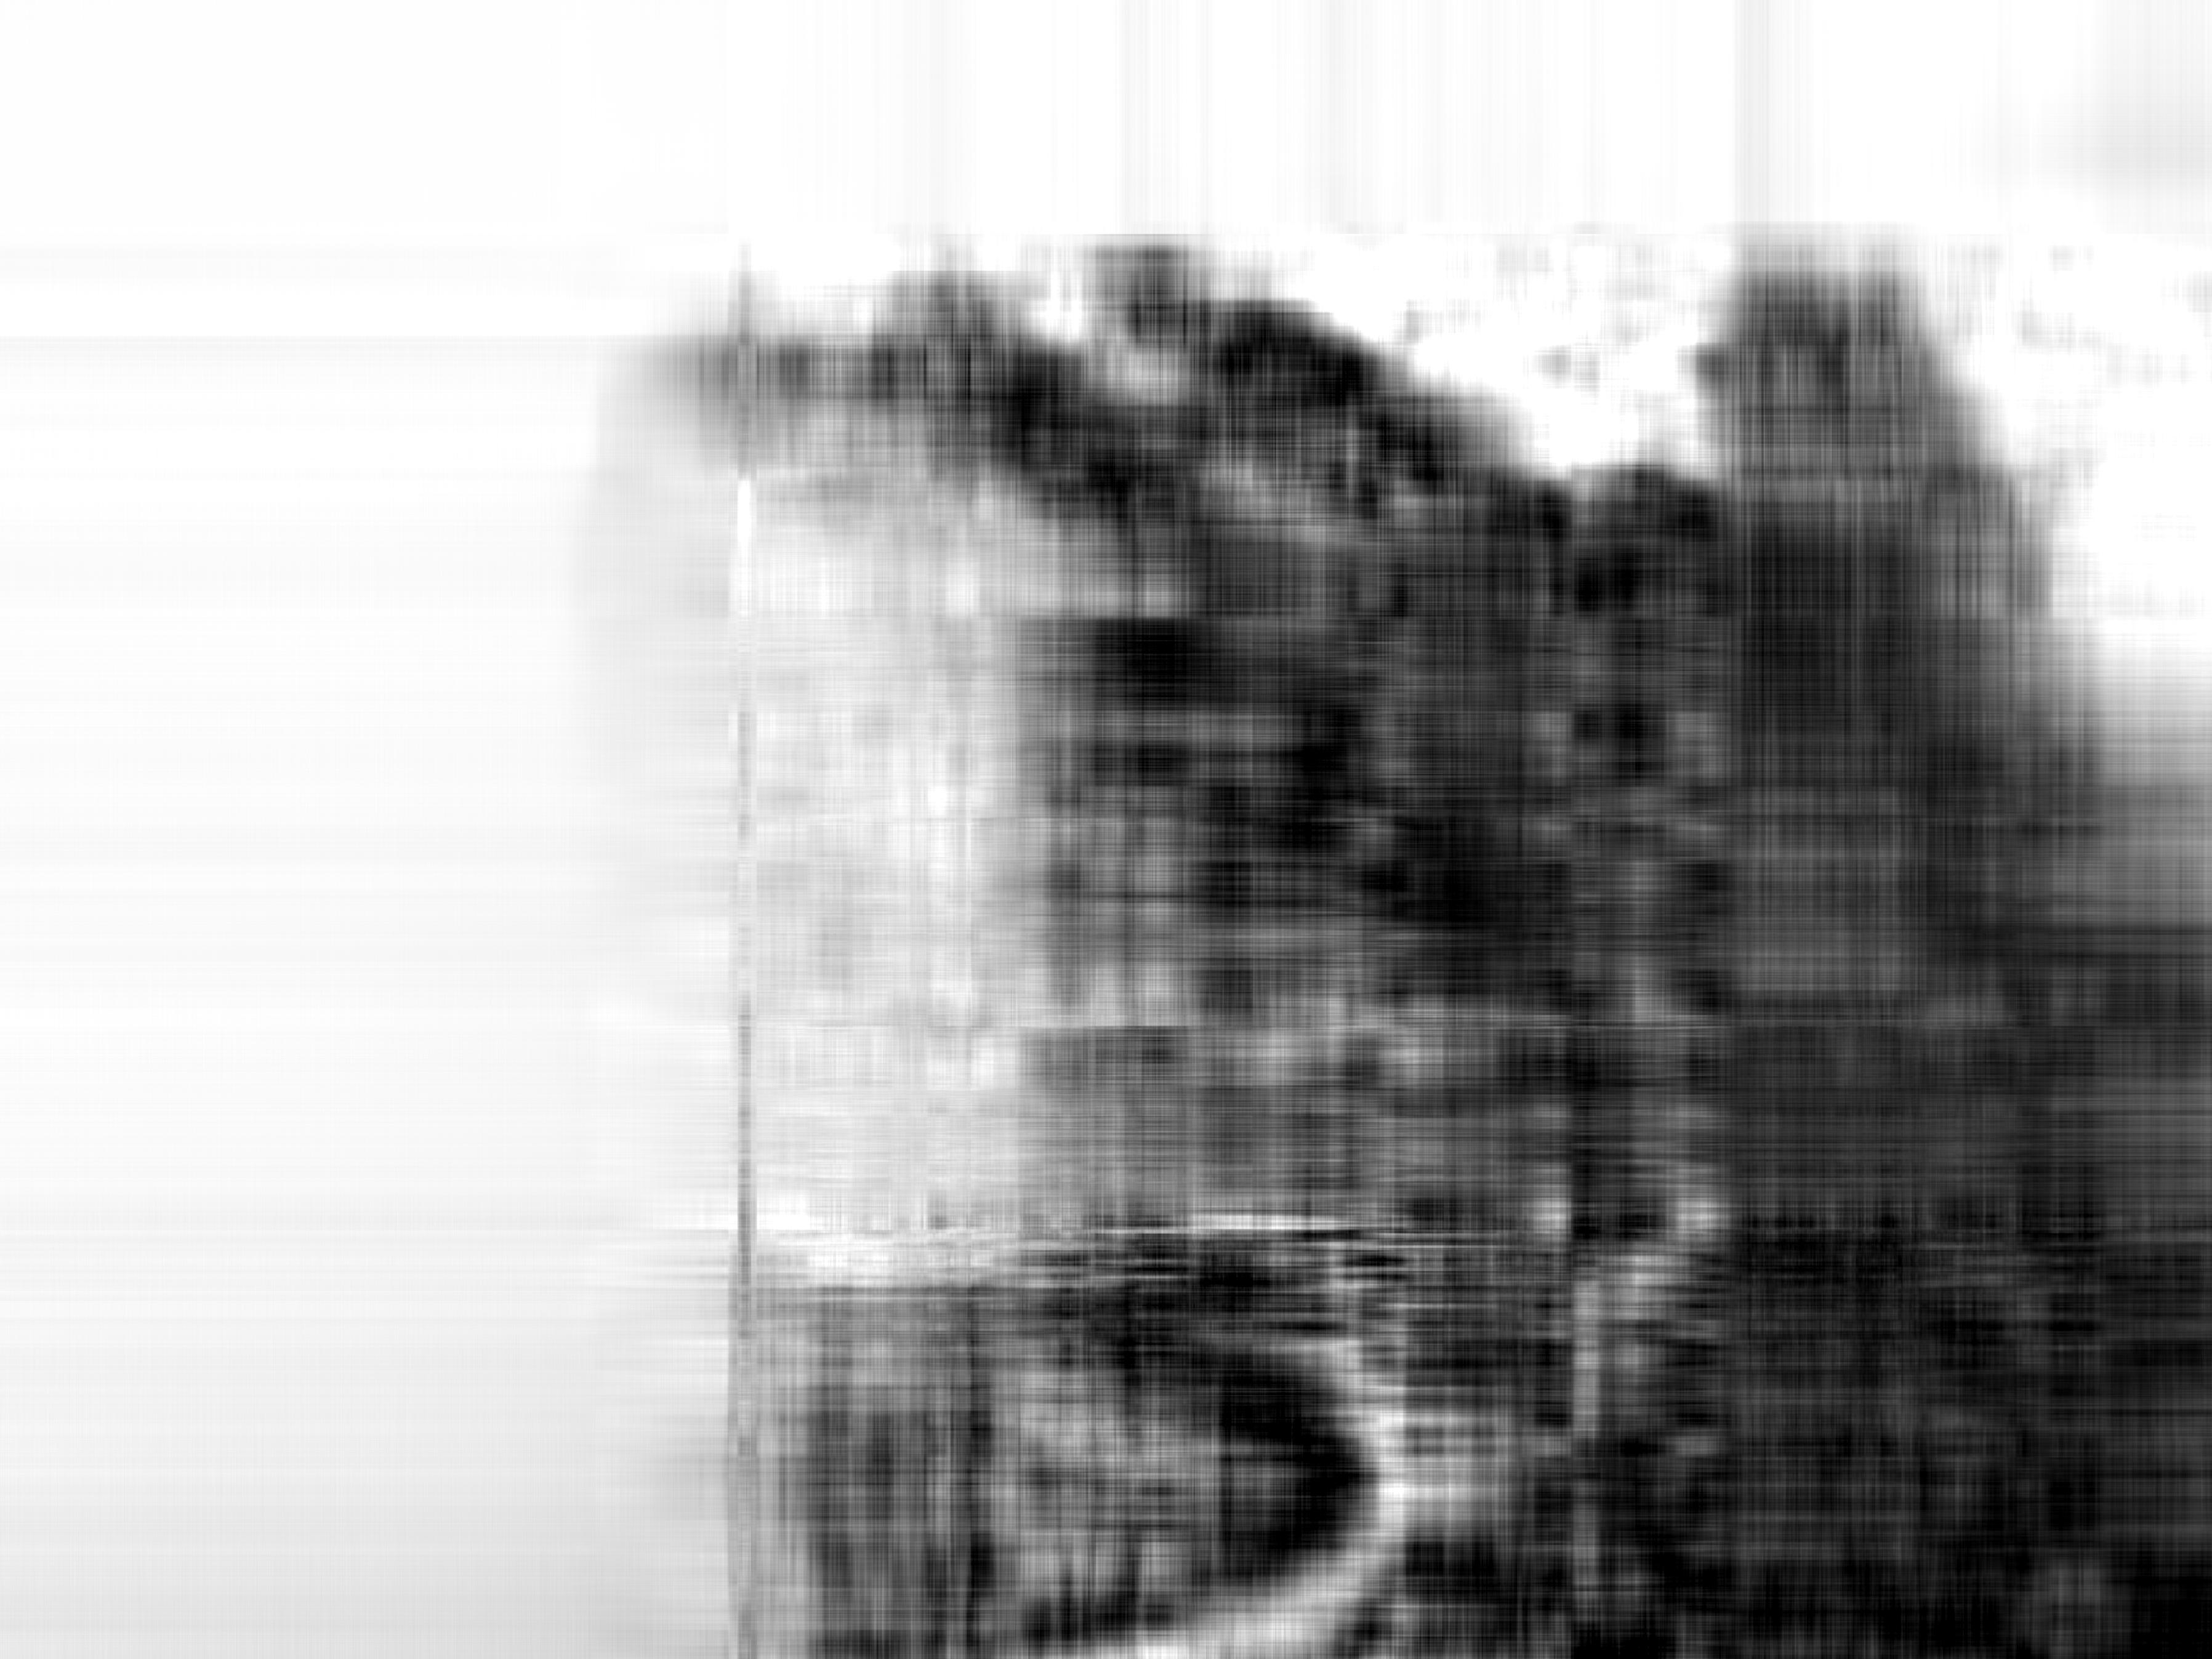
\includegraphics[width=0.5\textwidth]{./images/pca-4/photo-cliff-010.jpeg}
	}\parbox[b]{.5\textwidth}{		
		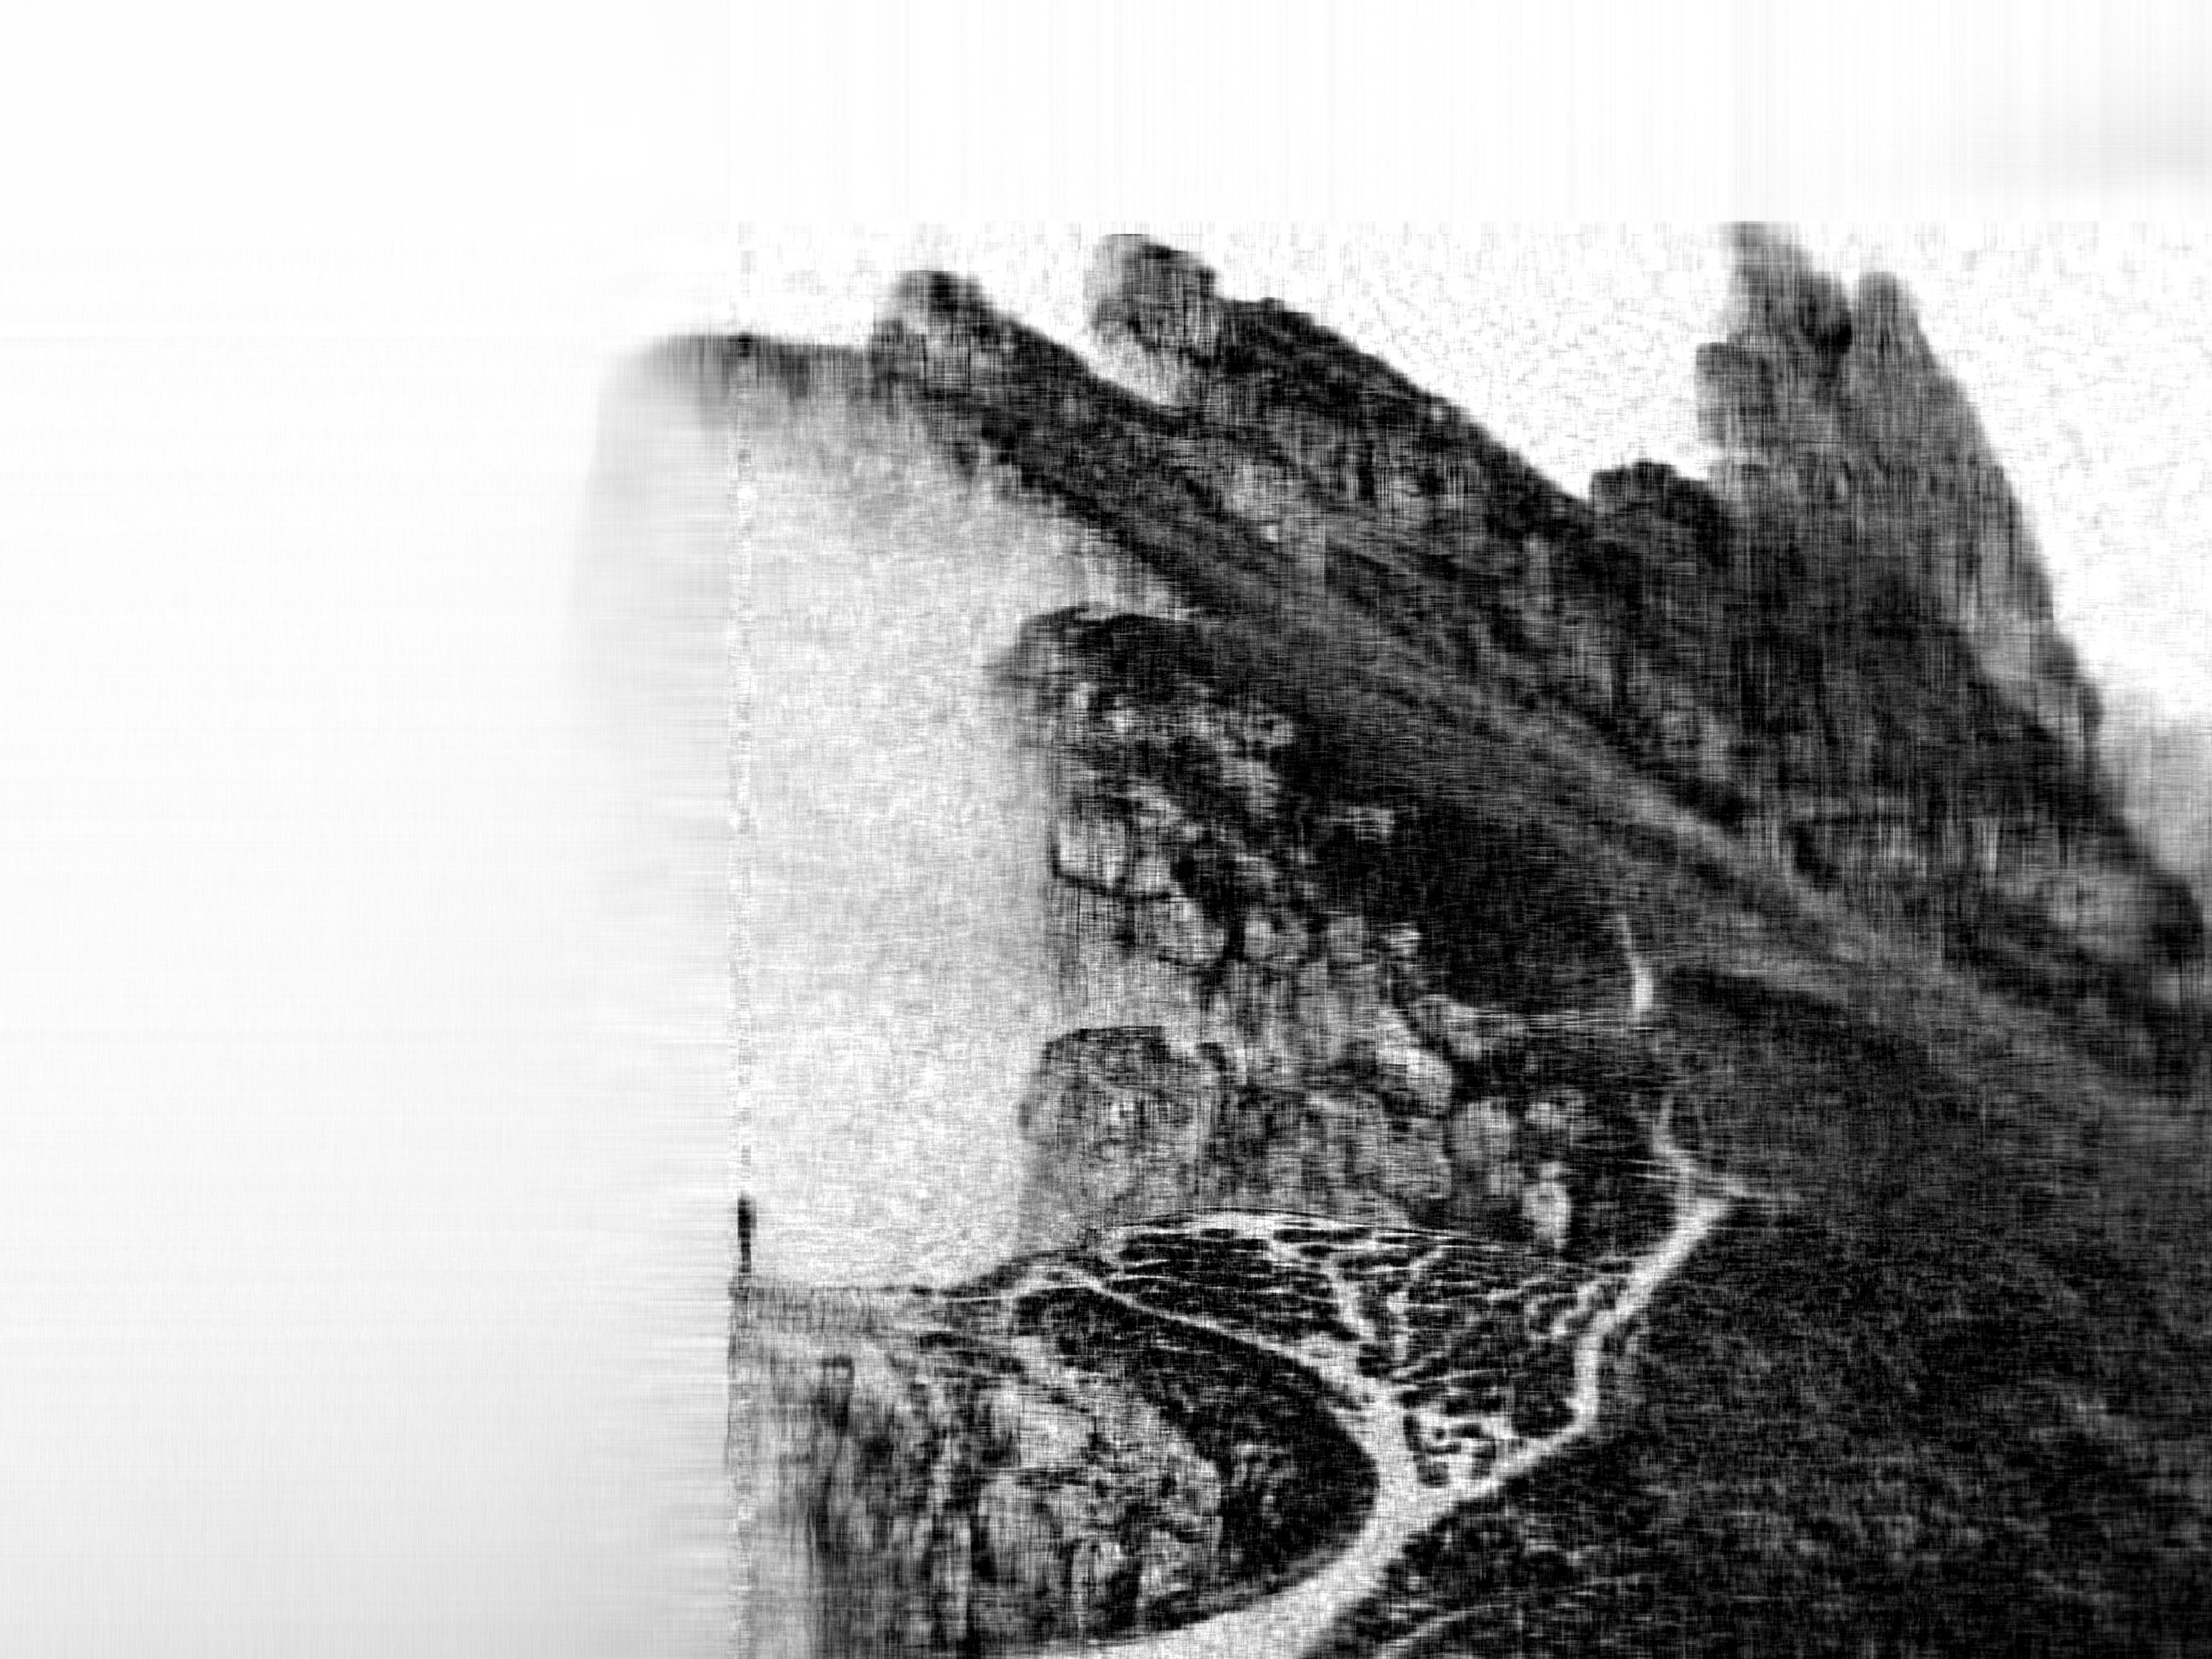
\includegraphics[width=0.5\textwidth]{./images/pca-4/photo-cliff-050.jpeg}
	}
	
	\parbox[b]{.5\textwidth}{	
		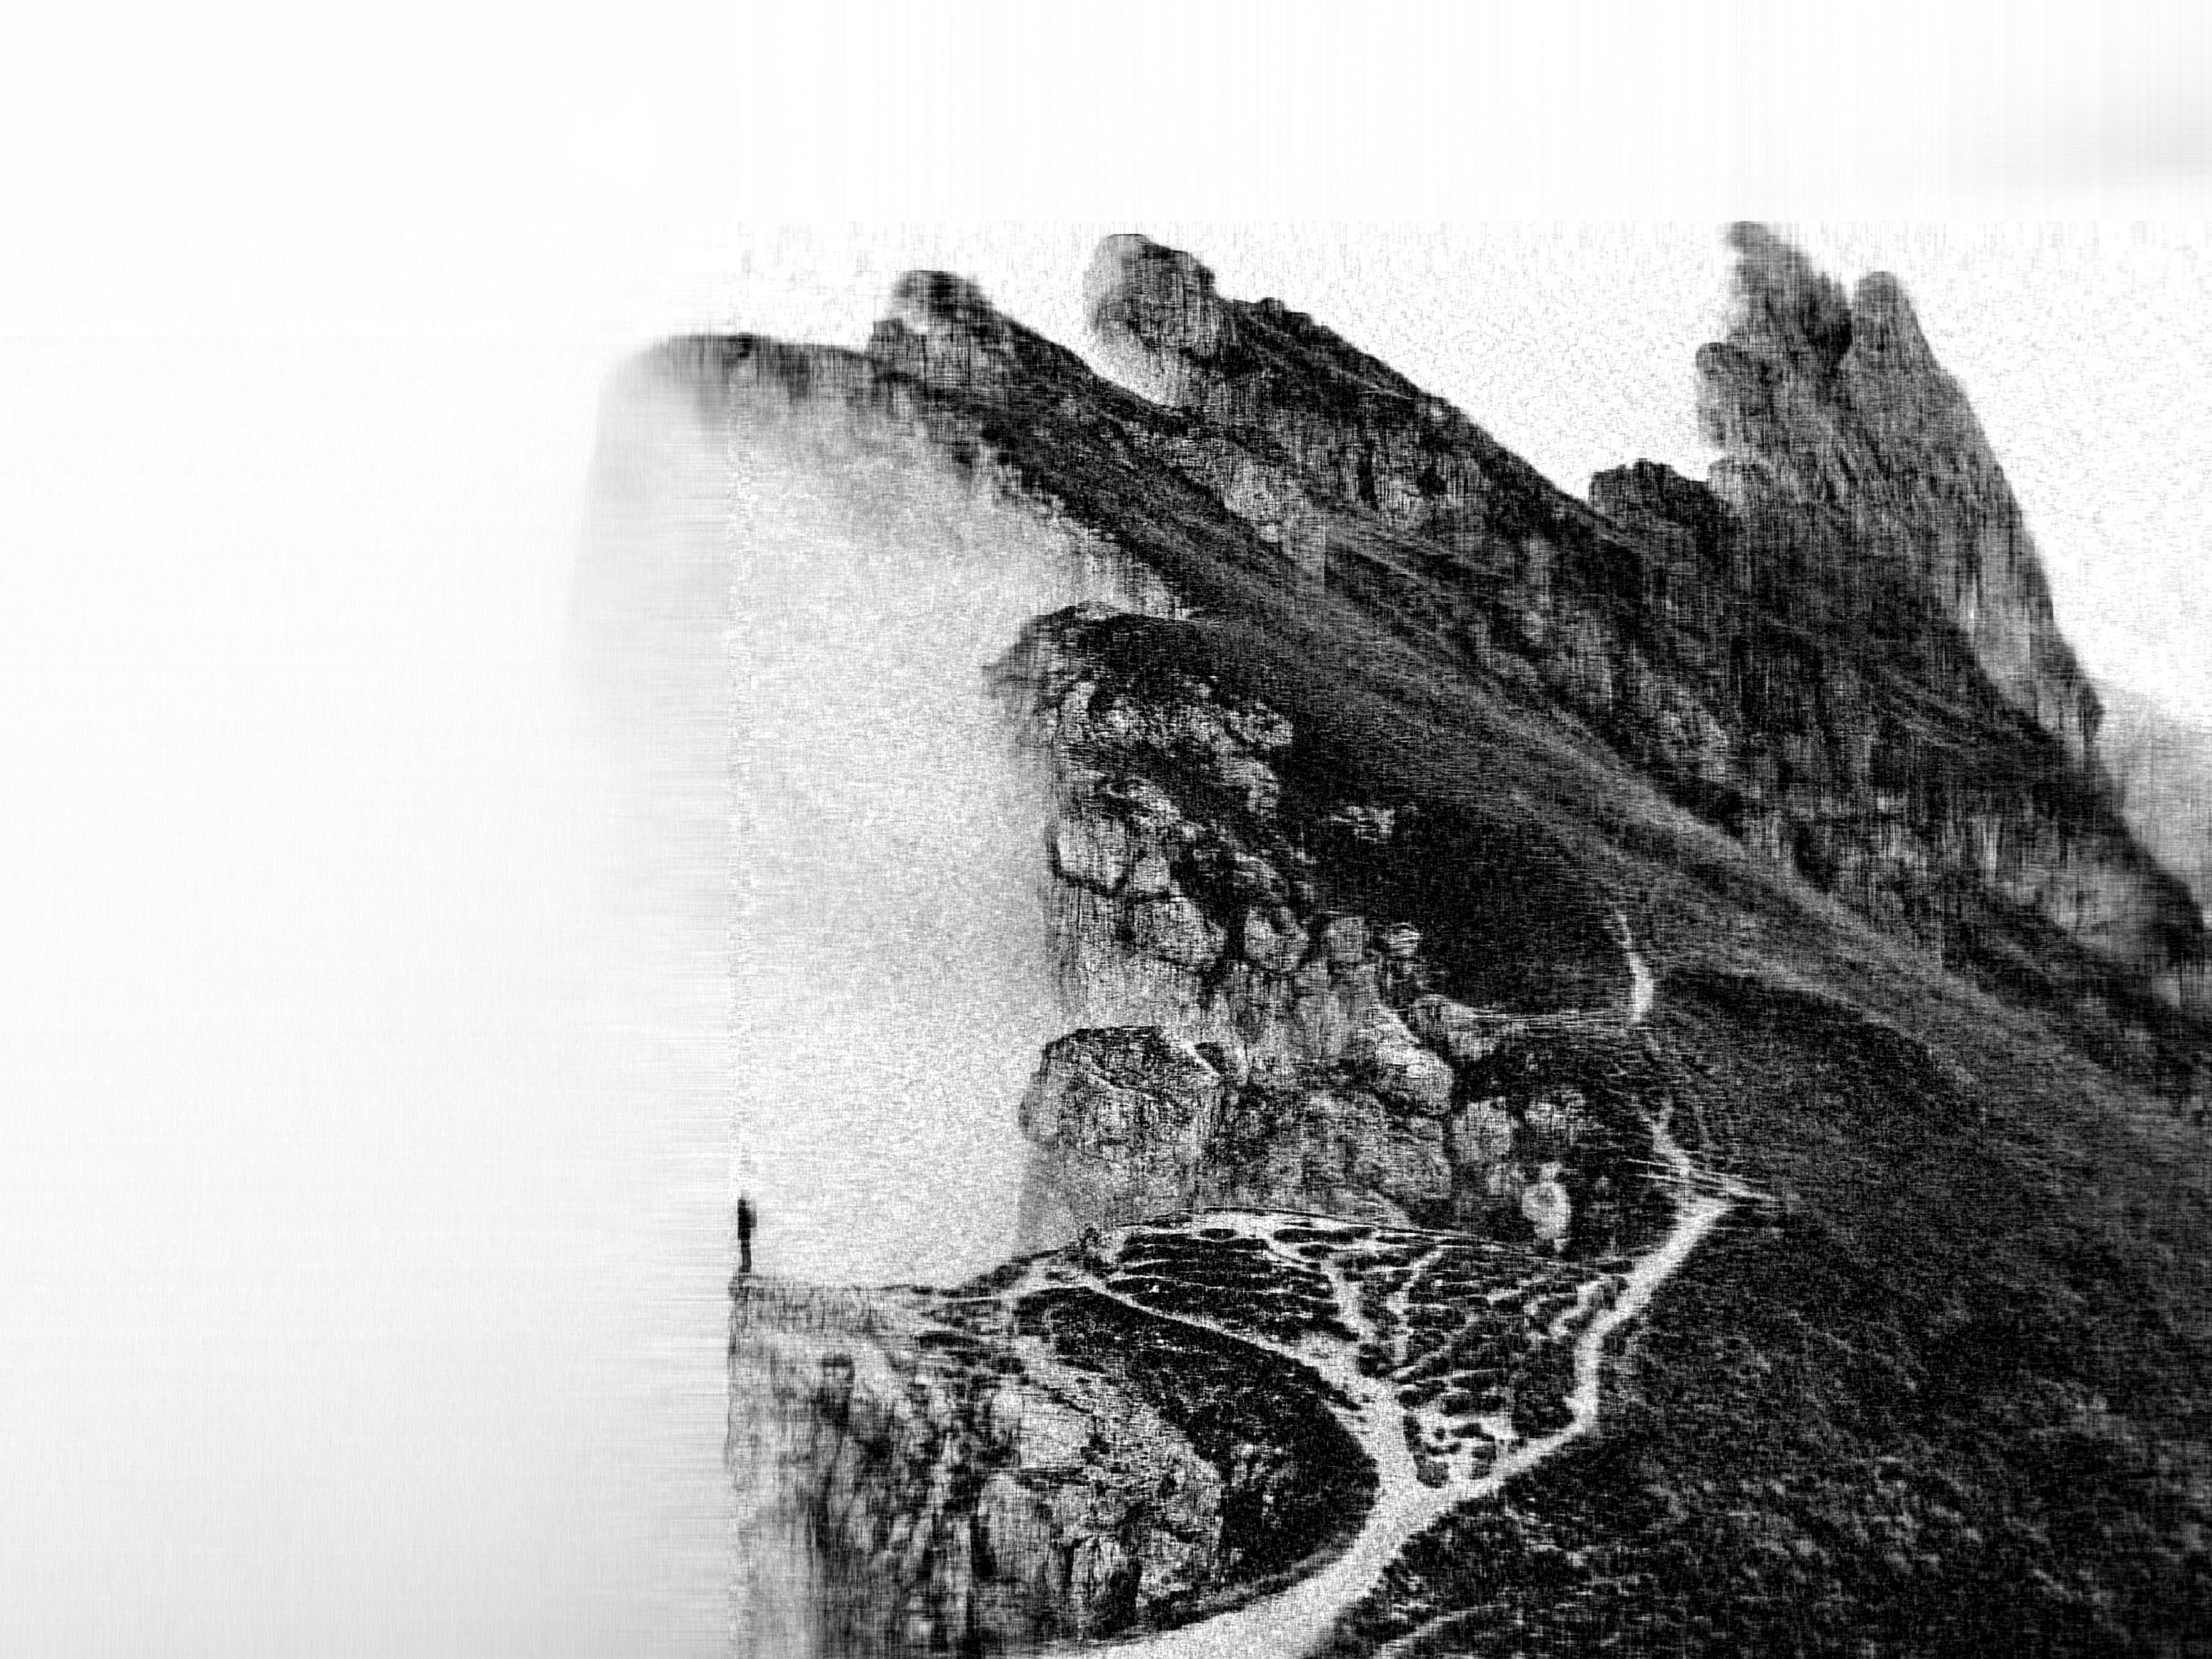
\includegraphics[width=0.5\textwidth]{./images/pca-4/photo-cliff-100.jpeg}
	}\parbox[b]{.5\textwidth}{		
		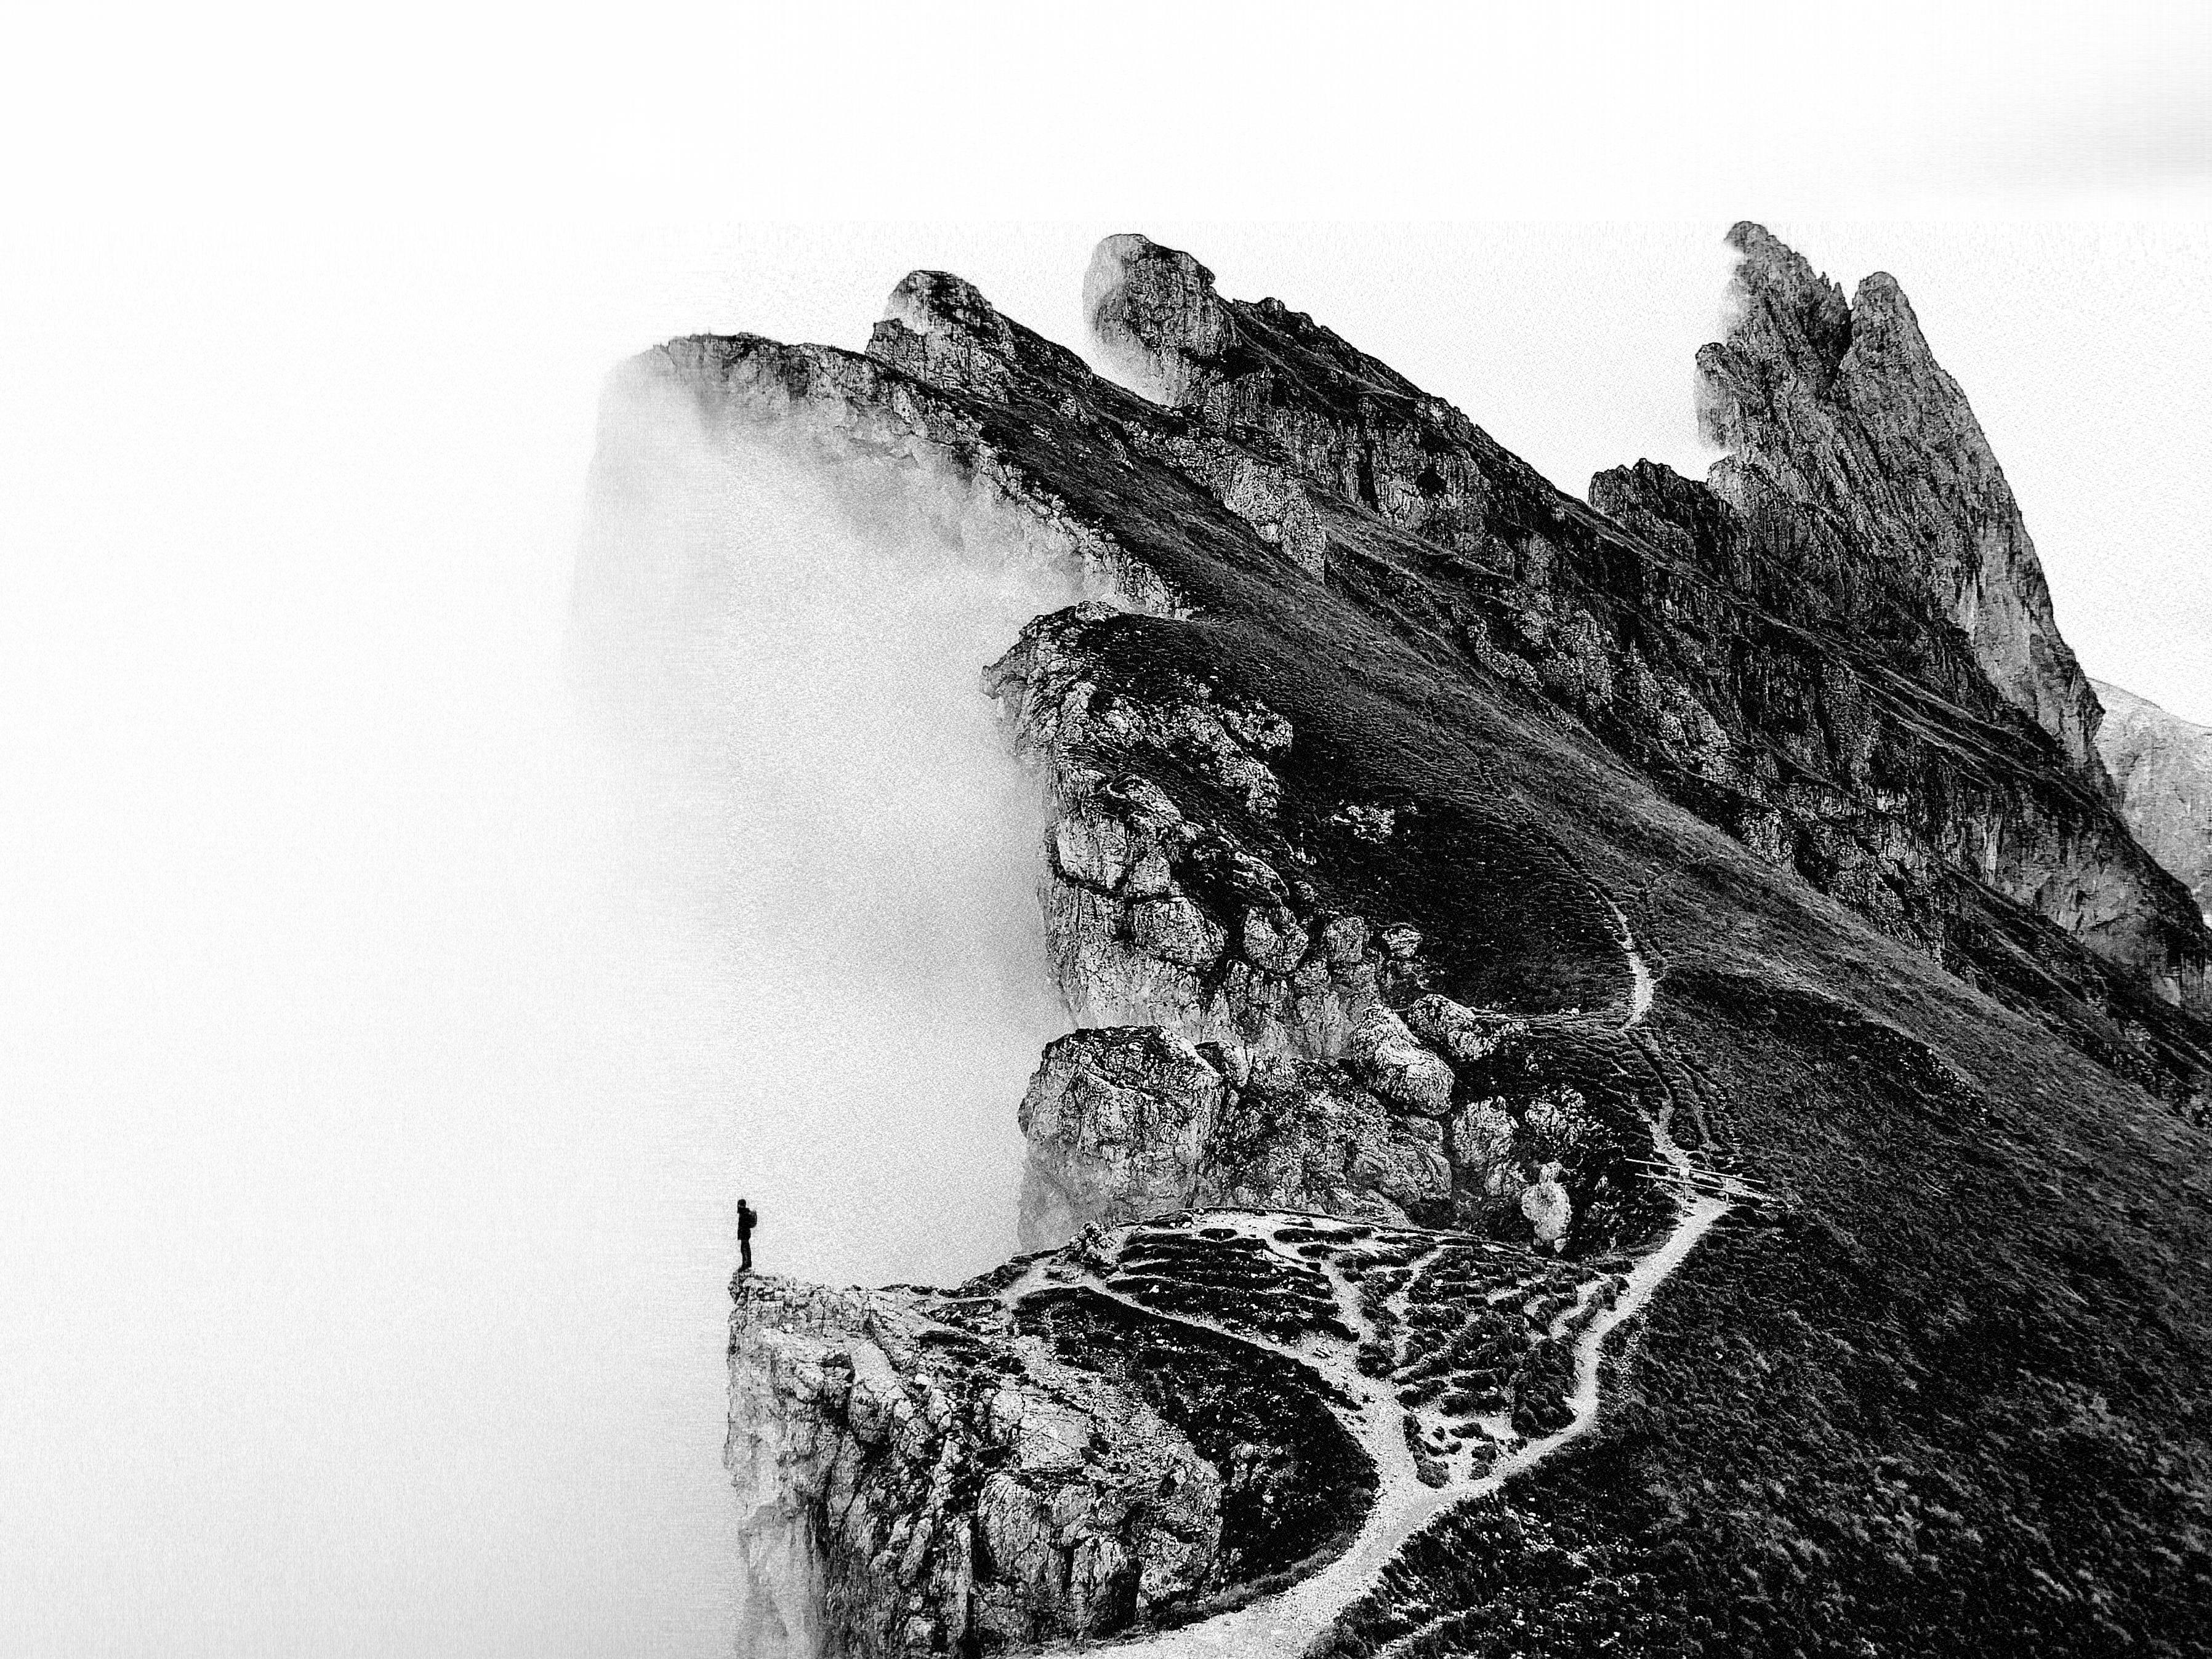
\includegraphics[width=0.5\textwidth]{./images/pca-4/photo-cliff-500.jpeg}
	}
	

	
	\caption*{Reconstructions of our image using 1, 2, 3, 5, 10, 50, 100 and 500 singular values and vectors.
	}
\end{figure}

%<figure class="wide">
%<img src="/images/pca-4/photo-cliff-001.jpeg" class="tile4"><img src="/images/pca-4/photo-cliff-002.jpeg" class="tile4"><img src="/images/pca-4/photo-cliff-003.jpeg" class="tile4"><img src="/images/pca-4/photo-cliff-005.jpeg" class="tile4">
%<img src="/images/pca-4/photo-cliff-010.jpeg" class="tile4"><img src="/images/pca-4/photo-cliff-050.jpeg" class="tile4"><img src="/images/pca-4/photo-cliff-100.jpeg" class="tile4"><img src="/images/pca-4/photo-cliff-500.jpeg" class="tile4">
%<figcaption>Reconstructions of our image using 1, 2, 3, 5, 10, 50, 100 and 500 singular values and vectors.</figcaption>
%</figure>

\begin{aside}To play around with this algorithm in color, see \href{http://timbaumann.info/svd-image-compression-demo}{this demo}\footnotemark by Tim Baumann.	
\end{aside}

\footnotetext{\url{http://timbaumann.info/svd-image-compression-demo}}

\subsection{Computing rank decompositions}

How good is this as an approximation of \(\gc{\mbM}\) using a rank decomposition? It turns out it's optimal. The \textbf{Eckart-Young-Mirsky theorem} tells us that no two rank-\(k\) matrices can multiply to produce a matrix that is closer than \(\mbA\mbB\). There are others that are equally close, but none are better.

\index{Eckart-Young-Mirsky theorem}

\pagebreak\noindent This sounds like another best-approximation theorem. The proof of this fact is pretty straightforward, but it doesn't illustrate how this relates to the best approximation results we've seen already. To make that link clear, we'll look at something a little short of a formal proof, which will hopefully provide more intuition into what is happening when we approximate a matrix this way.

First, let's state the problem formally. We are looking for two matrices \(\bc{\mbA}\) and \(\rc{\mbB}\) with sizes \(n \times k\) and \(k \times m\) so that
\[\| \bc{\mbA}\rc{\mbB} - \gc{\mbM} \|\]
is as small as possible.

\begin{aside}We're using a matrix norm here called the Frobenius norm. That sounds fancy, but we're just talking about the Euclidean distance between \(\bc{\mbA}\rc{\mbB}\) and \(\gc{\mbM}\) that you would get if you flattened both matrices into vectors.	
\end{aside}

\index{Frobenius norm}
\index{Matrix norm}
\index{$\|\gc{\mbM}\|$}


This is a \emph{bi-linear} minimization objective. If we fix \(\bc{\mbA}\), we can use what we already know about linear problems to find the optimal \(\rc{\mbB}\) and vice versa. To illustrate, let's first assume that the optimal \(\bc{\mbA}\) is given and we only need to find \(\rc{\mbB}\).

\index{Bi-linear optimization}

To apply what we've learned about the pseudo-inverse, we can proceed column by column. Looking at a matrix multiplication, we know that whatever \(\rc{\mbB}\) we choose, the \(i\)-th column of \(\rc{\mbB}\) multiplies by \(\bc{\mbA}\) to make the \(i\)-th column of \(\gc{\mbM}\): \(\bc{\mbA}\rc{\mbb}_i = \gc{\mbm}_i\).

\enlargethispage{2em}

\begin{figure}[H]
	\centerline{
		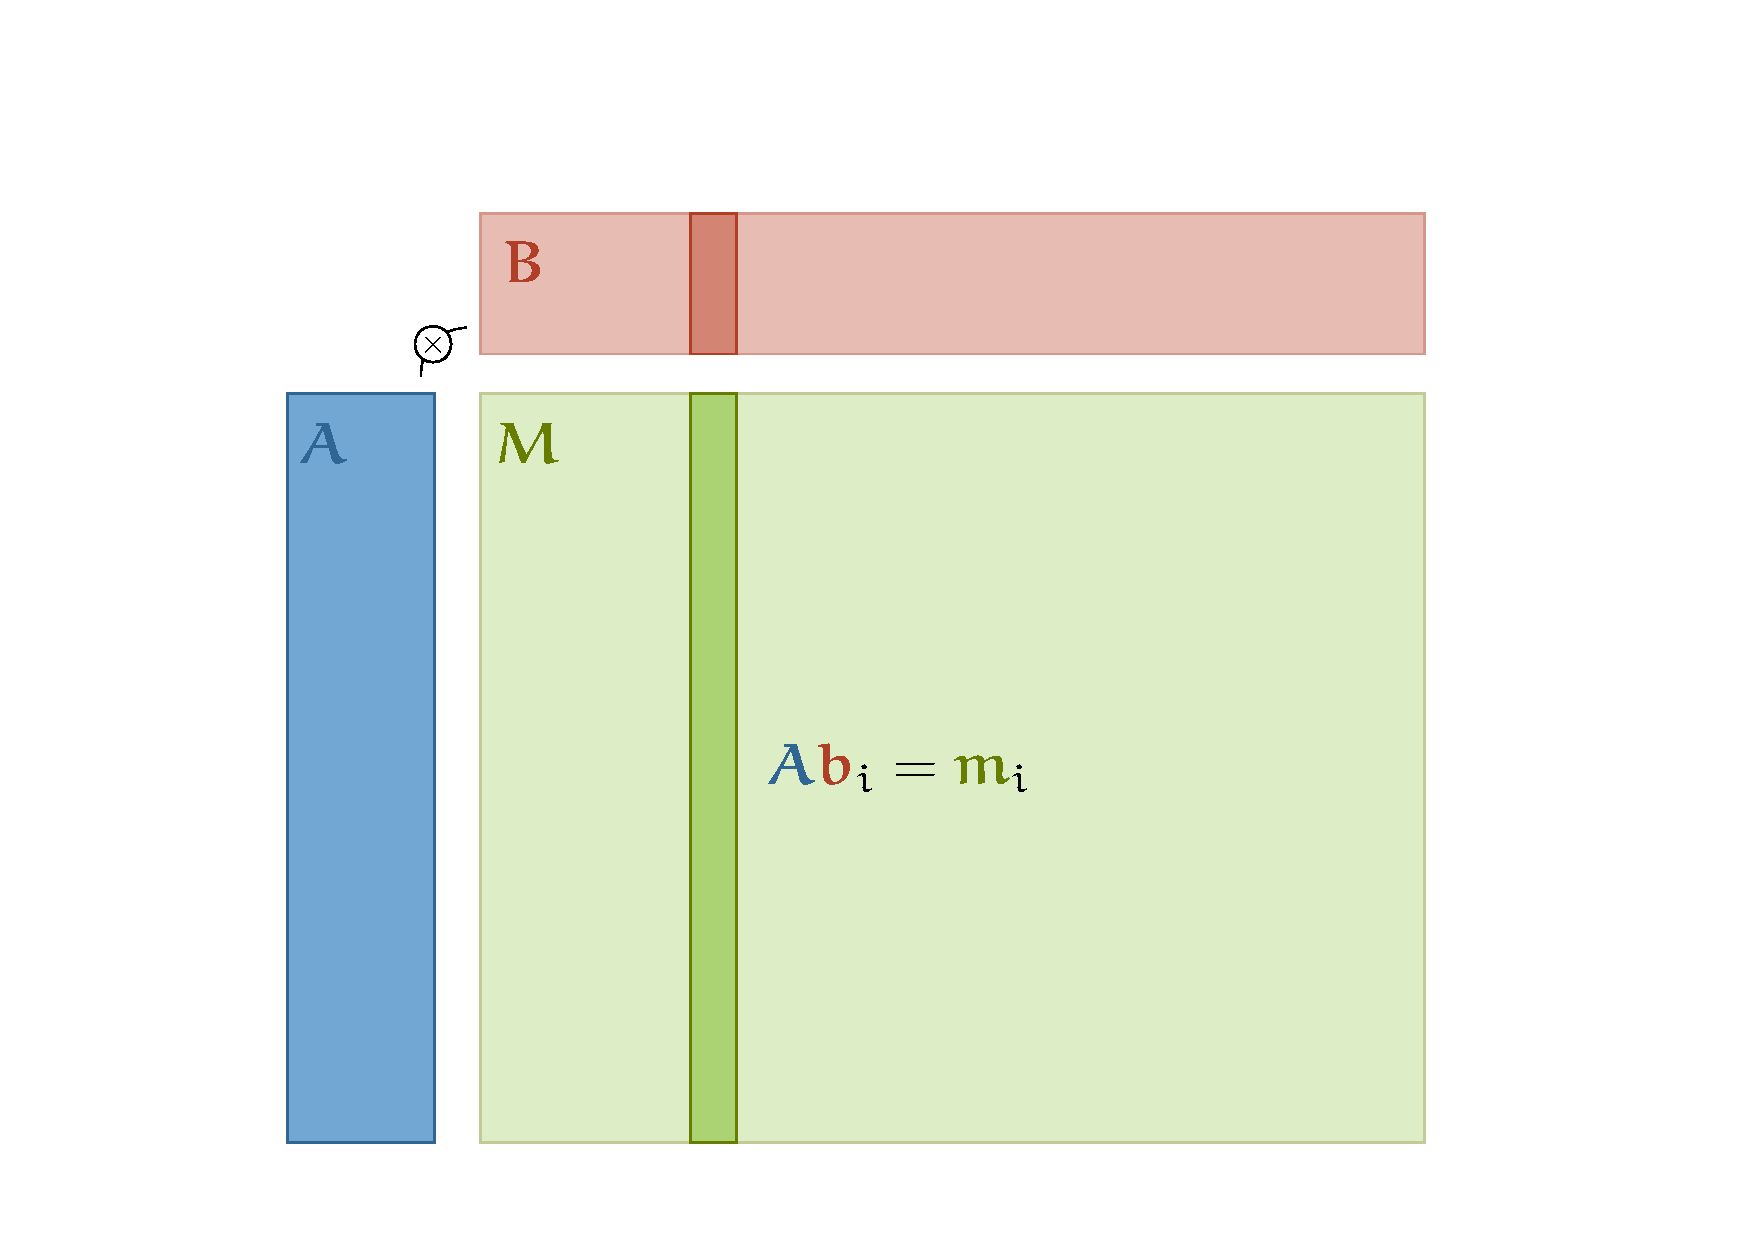
\includegraphics[width=0.6\textwidth]{./images/pca-4/decomp-col.pdf}
	}
\end{figure}

%<figure class="narrow centering">
%<img src="/images/pca-4/decomp-col.svg" class="three-quarters">
%</figure>

This is entirely independent of what we choose for the other columns: if we change something in \(\rc{\mbb}_i\), only \(\gc{\mbm}_i\) is affected. Thus, we can treat this as a separate optimization problem for each column, and apply the pseudo-inverse to each. The solution is
\[
\rc{\mbb}_i = \bc{\mbA}^\dagger\gc{\mbm}_i \p
\]

If we combine the columns \(\rc{\mbb}_i\) back into a matrix, we get
\[
\rc{\mbB} = \left[\,\rc{\mbb}_1\,\ldots \,\rc{\mbb}_m\,\right] = \left[\,\bc{\mbA}^\dagger\gc{\mbm}_1 \,\ldots\, \bc{\mbA}^\dagger\gc{\mbm}_m\,\right] = \bc{\mbA}^\dagger \gc{\mbM} \p
\]

In short, solving \(\bc{\mbA}\rc{\mbB} = \gc{\mbM}\) for \(\rc{\mbB}\), we find that \(\rc{\mbB} = \bc{\mbA}^\dagger\gc{\mbM}\). We take \(\bc{\mbA}\) to the other side using the pseudo-inverse, analogous to the way we would solve a scalar equation.

If we reverse the setting, and assume that \(\rc{\mbB}\) is given, we can take the transpose of all matrices so that our objective becomes 
\[\| \rc{\mbB}^T\bc{\mbA}^T - \gc{\mbM}^T \|\p\]

We can then follow the same derivation as above, finding that the \emph{rows} of \(\bc{\mbA}\) multiply by \(\rc{\mbB}^T\) to make the rows of \(\gc{\mbM}\). Ultimately, the optimal choice of \(\bc{\mbA}\) becomes
\[\bc{\mbA} = \gc{\mbM}\rc{\mbB}^\dagger \p\]

This gives us two equations that should hold at the optimum. We can now show that the SVD solution to the rank decomposition problem we described above satisfies these equations.

First, we take the SVD of \(\gc{\mbM}\) truncated at \(k\):

\[\gc{\mbM} \approx \rc{\mbU}\gc{\Sig}\rc{\mbV}^T \p\]

We've ommitted the subscripts for clarity, but note that \(\rc{\mbU}\) is \(n \times k\), \(\gc{\Sig}\) is \(k \times k\) and \(\rc{\mbV}\) is \(m \times k\).

If we define \(\bc{\mbA} = \rc{\mbU}\gc{\Sig}^\frac{1}{2}\) and \(\rc{\mbB} = \gc{\Sig}^\frac{1}{2}\rc{\mbV}^T\) then they combine into a low rank approximation of \(\gc{\mbM}\) as we already showed. What we can also conclude is that this gives us the SVD decompositions of \(\bc{\mbA}\) and \(\rc{\mbB}\). All we need is to add a \(k \times k\) identity matrix:
%
\begin{align*}
\bc{\mbA} &= \rc{\mbU}\gc{\Sig}^\frac{1}{2}\rc{\mbI}^\kc{T} \\
\rc{\mbB} &= \rc{\mbI}\gc{\Sig}^\frac{1}{2}\rc{\mbV}^T \p
\end{align*}

This in turn, tells us what the pseudo-inverses of \(\bc{\mbA}\) and \(\rc{\mbB}\) are.
\begin{align*}
\bc{\mbA}^\dagger &= \rc{\mbI}\gc{\Sig}^{-\frac{1}{2}}\rc{\mbU}^T \\
\rc{\mbB}^\dagger &= \rc{\mbV}\gc{\Sig}^{-\frac{1}{2}}\rc{\mbI}^\kc{T} \p
\end{align*}

We can now simply fill in these definitions to show that the required equations hold for this choice of \(\bc{\mbA}\) and \(\rc{\mbB}\). For \(\bc{\mbA}\) we get
%
\begin{align*}
\bc{\mbA} &= \rc{\mbU}\gc{\Sig}^\frac{1}{2}\rc{\mbI}^\kc{T} \\
&= \rc{\mbU}\gc{\Sig}\gc{\Sig}^{-\frac{1}{2}}\rc{\mbI}^\kc{T}\\
&= \rc{\mbU}\gc{\Sig}\rc{\mbV}^T\rc{\mbV}\gc{\Sig}^{-\frac{1}{2}}\rc{\mbI}^\kc{T}\\
&= \gc{\mbM}\rc{\mbB}^\dagger \p
\end{align*}

And for \(\rc{\mbB}\)
%
\begin{align*}
\rc{\mbB} &= \rc{\mbI}\gc{\Sig}^\frac{1}{2}\rc{\mbV}^T \\
&= \rc{\mbI}\gc{\Sig}^{-\frac{1}{2}}\gc{\Sig}\rc{\mbV}^T \\
&= \rc{\mbI}\gc{\Sig}^{-\frac{1}{2}}\rc{\mbU}^T\rc{\mbU}\gc{\Sig}\rc{\mbV}^T \\
&= \bc{\mbA}^\dagger\gc{\mbM}\p
\end{align*}

This isn't a complete proof. We have only shown that one necessary condition holds. To complete the proof, we should show that this condition is also sufficient. This is possible, but a bit technical. Instead, we'll wait until we tie this back into principal component analysis, in the next subsection. There, we will see that the results we already know will serve as a proof of the Eckart-Young-Mirsky theorem.

So, in summary, the SVD gives us a very efficient way to approximate matrices by compressed representations. We started with image compression as a use case, because it's a visual example. But there are many other situations where our data forms a matrix, and in any such case, the rank decomposition, computed by SVD, provides us with an efficient mechanism to separate pattern from noise. Either for compression, analysis or for prediction.

\subsection{Recommendation}

One particularly relevant and popular example is that of \textbf{recommendation}. This is where we see that the SVD can be a powerful tool for \emph{prediction}.

\index{Recommendation}

Imagine that you are running a movie streaming service. You have a large collection of \bc{movies} and a large population of \oc{users}.

Each user has given you a few ratings for a small subset of the movies. This rating consists of a high positive number if they like the movie, a high negative number if they dislike the movie and something near zero if they were ambivalent.

\begin{aside}That's not usually how users rate things, but it's the simplest setting for us. We can worry about mapping a real user rating to this scale later.	
\end{aside}


If we have \(\oc{n}\) users, and \(\bc{m}\) movies, we can put these ratings in a big \(\oc{n} \times \bc{m}\) matrix \(\mbR\). The element \(R_{\oc{i}\bc{j}}\) tells us what user \(\oc{i}\) thought of movie \(\bc{j}\). For some pairs \(\oc{i}, \bc{j}\), we don't have a rating (if we knew the whole matrix, we wouldn't need a recommender). For now, we'll set these elements of the matrix to zero, and see what we can do.

\enlargethispage{2em}

Let's see what happens if we apply a rank decomposition to the matrix \(\mbR\). We'll get one \(\oc{n} \times k\) matrix \(\oc{\mbU}\), and one \(\bc{m} \times k\) matrix \(\bc{\mbM}\) such that \(\mbR \approx \oc{\mbU}\bc{\mbM}^T\).


\begin{figure}[H]
	\centerline{
		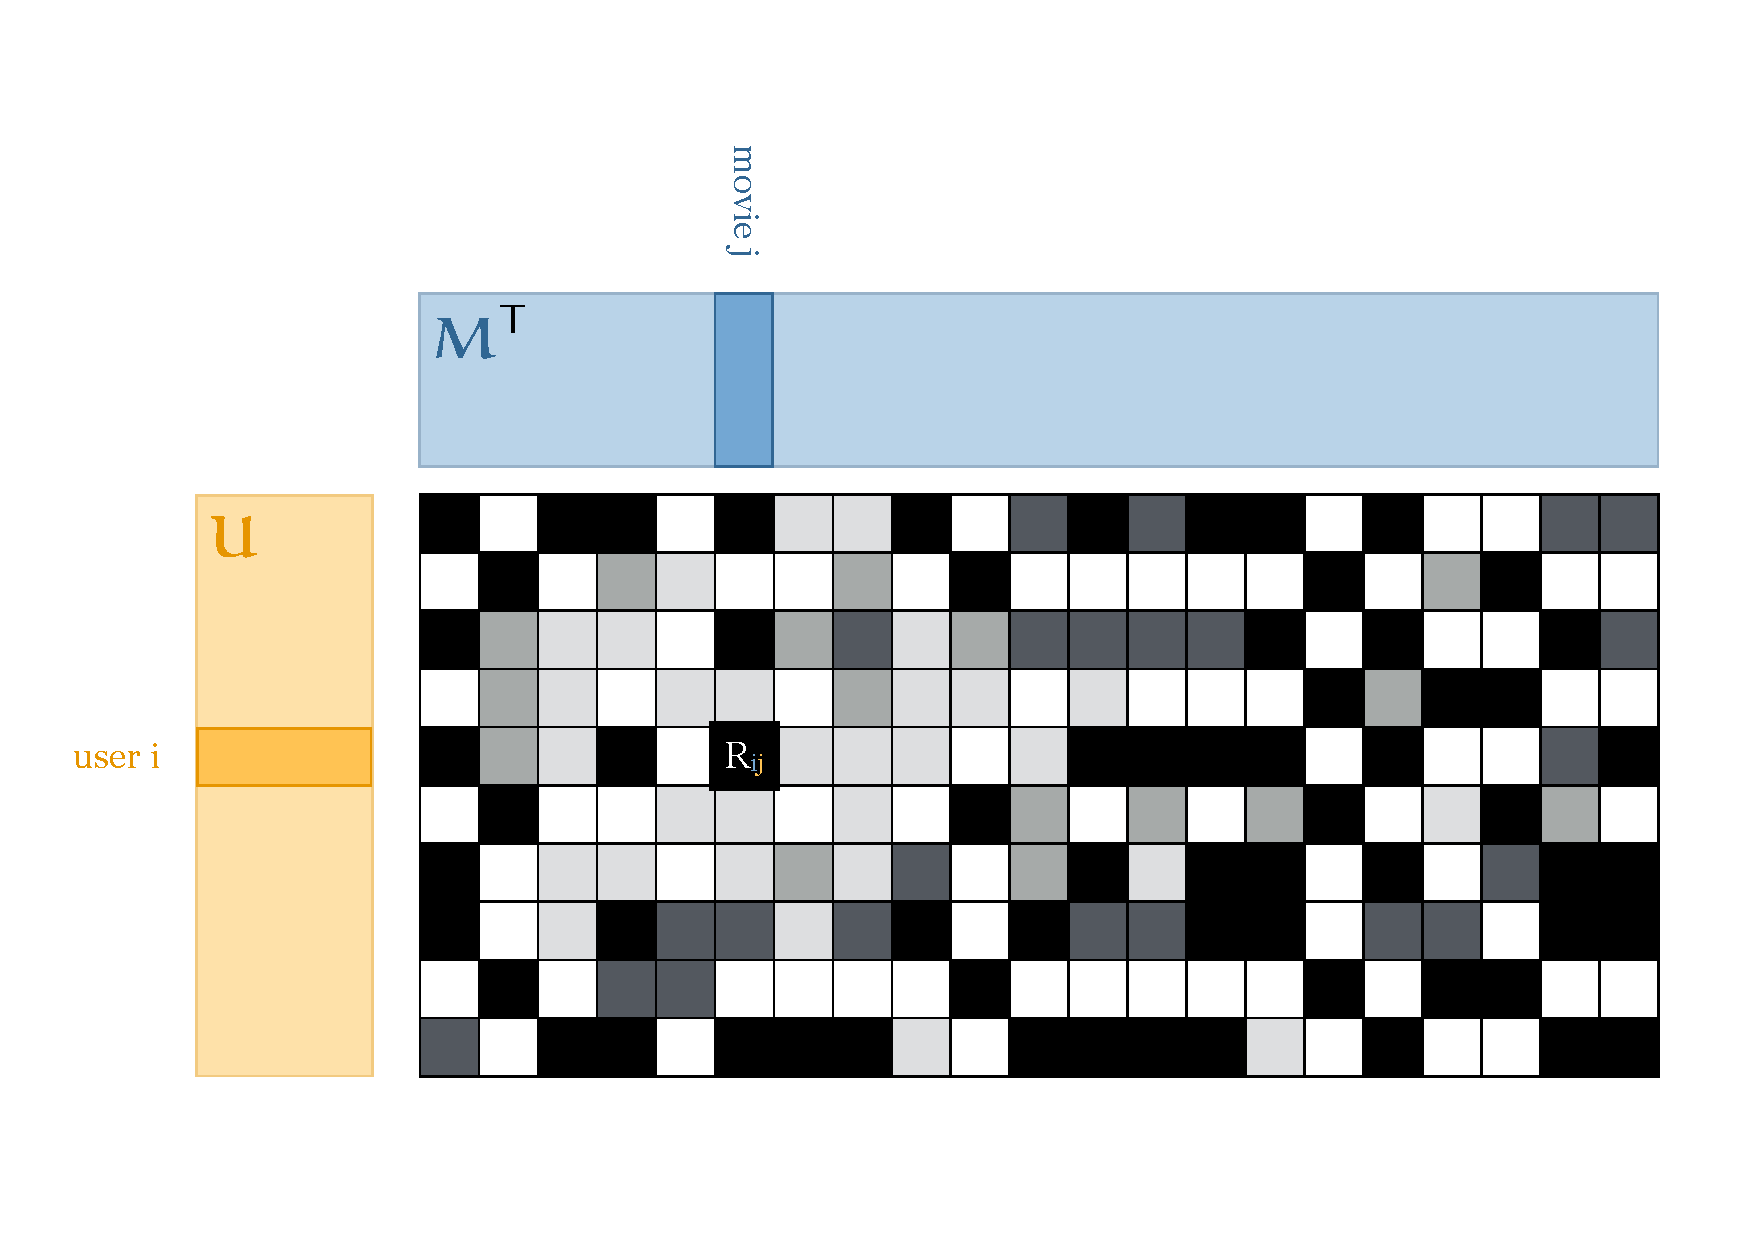
\includegraphics[width=1\textwidth]{./images/pca-4/movieratings.pdf}
	}
\end{figure}

%<figure class="narrow centering">
%<img src="/images/pca-4/movieratings.svg">
%</figure>

We can think of the \(\oc{i}\)-th row of \(\oc{\mbU}\) as a representation of the \(\oc{i}\)-th user and the \(\bc{j}\)-th row of \(\bc{\mbM}\) as a representation of the \(\bc{j}\)-th movie. Their dot product is the approximation to the rating \(R_{\oc{i}\bc{j}}\). The basic idea of this kind of recommendation is that if \(R_{\oc{i}\bc{j}}\) approximates the known ratings well, then it may approximate the unknown ratings too. We can think of \(R_{\oc{i}\bc{j}}\) as a \emph{prediction} for whether user \(\oc{i}\) will like movie \(\bc{j}\).

\begin{aside}Of course, we're now also explicitly optimizing for the prediction to be \(0\) for these entries, so something slightly counter-intuitive is happening here, but in practice the way the algorithm deviates from these \(0\)'s is still predictive. We'll see a fix for this later.	
\end{aside}


What might a good solution to this problem look like? Here's one way to think about it. Imagine that we were to fill in the user representation \(\oc{\mbu}\) and the movie representation \(\bc{\mbm}\) by hand, in such a way that their dot product would be positive if the user likes the movie and negative if the user dislikes the movie.

One way to do this is to come up with \(k\) features a movie can have, like comedy, drama and romance. You can score the movie on each aspect, giving it for instance, a large negative score if for comedy if the movie is highly un-comedic and a zero for romance if the movie is neither romantic nor unromantic.

We can then score the user in a similar way based on how much they like these aspects. If the used loves comedy, we give them a large score for comedy. If they hate romance, we give them a large negative score for romance, and if they are ambivalent about drama, we give them a zero for drama.

\enlargethispage{2em}
\begin{figure}[H]
	\centerline{
		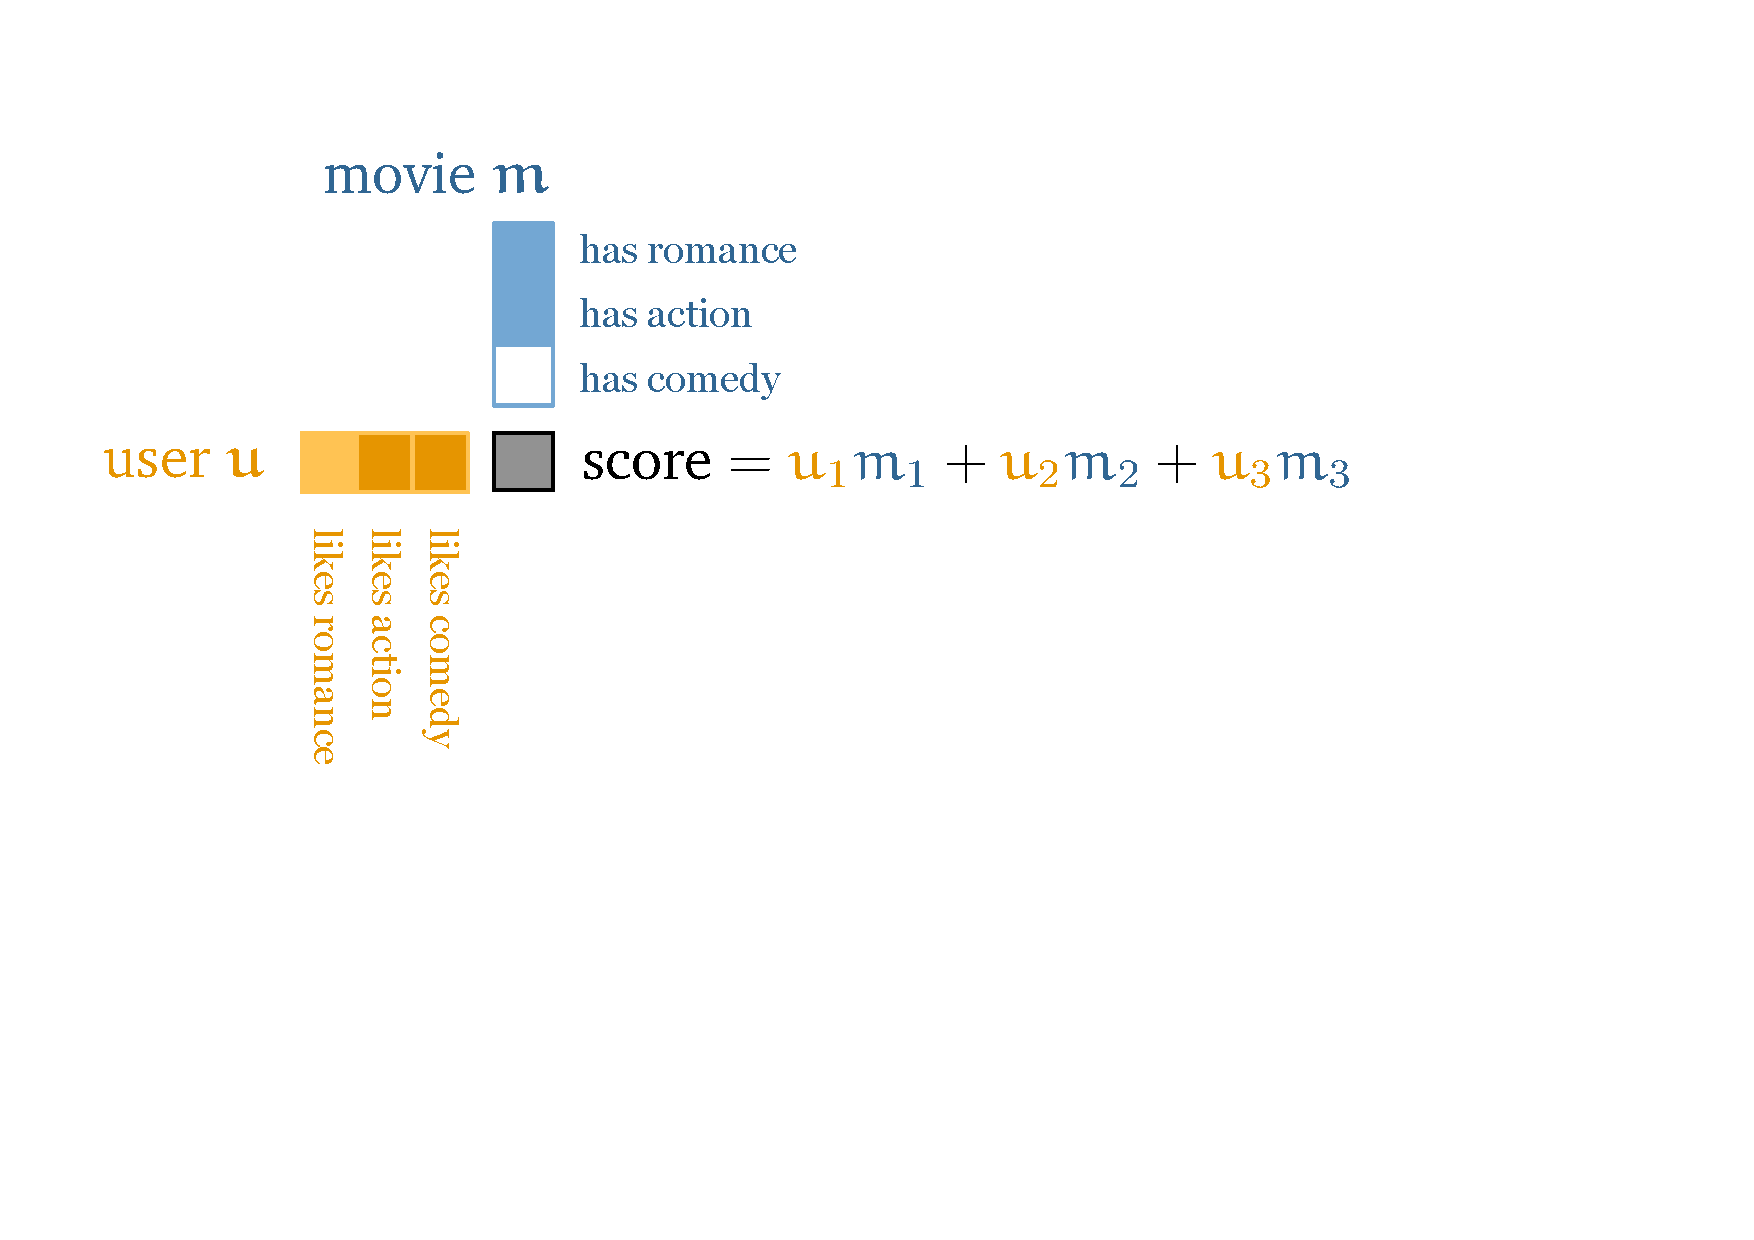
\includegraphics[width=0.85\textwidth]{./images/pca-4/dotprod.pdf}
	}
\end{figure}

%<figure class="narrow centering">
%<img src="/images/pca-4/dotprod.svg">
%</figure>

If we have all this information for the user and the movie, then we can see that the dot product is a great predictor for how much the user will like the movie.

Note that if two aspects have the same sign: the user likes romance and the movie contains it, or the user hates romance and the movie is unromantic, both lead to a higher score. Similarly, if two aspects have opposite signs the score is lowered. Finally, note that if one aspect is near zero, that aspect does not affect the score. For instance, if the user is ambivalent about the amount of romance, it doesn't matter for the score whether or not the movie contains a lot or romance or is totally unromantic.

In practice, we don't have the means to collect all this information for our users and movies. Instead, we collect ratings, and we \emph{learn} the representations for our users and movies by decomposing the rating matrix. 

The surprising thing is that matrix decomposition still learns intepretable features. Here are the first two dimensions in this learned space from a simple matrix decomposition of a movie rating dataset.

\begin{figure}[H]
	\centerline{
		\includesvg[width=0.8\textwidth]{./images/pca-4/movie-features.svg}
	}
	\caption*{
	The first two dimensions of a movie representation learned by matrix decomposition, from \cite{koren2009matrix}. 
	%It's not clear from the paper exactly which decomposition was used for this specific image, but it will be something close to a rank decomposition.
	}
\end{figure}

%<figure class="narrow centering">
%<img src="/images/pca-4/movie-features.svg">
%<figcaption>
%The first two dimensions of a movie representation learned by matrix decomposition. From <a href="https://datajobs.com/data-science-repo/Recommender-Systems-[Netflix].pdf">Matrix factorization techniques for recommender systems</a> by Yehuda Koren et al. It's not clear from the paper exactly which decomposition was used for this specific image, but it will be something close to a rank decomposition.
%</figcaption>
%</figure>

This is an interesting takeaway of the recommender system use case: it shows us how we can interpret the rows of the two matrices we've decomposed \(\mbR\) into. In general, if we decompose \(\gc{\mbM}\) into \(\bc{\mbA}\rc{\mbB}\), then the \(i\)-th row of \(\bc{\mbA}\) is a vector representation of the element represented in the \(i\)-th row of \(\gc{\mbM}\). In movie recommendation, this is the \(i\)-th user, and in image compression, it's something more abstract like the \(i\)-th row of pixels. Likewise, the \(j\)-th column of \(\rc{\mbB}\) is a learned representation of whatever the \(j\)-th column of \(\gc{\mbM}\) represents.

The hyperparameter \(k\) gives us a classic under/overfitting tradeoff. For low \(k\), we have little space to model many aspects of our users and movies. We won't fit much of the pattern in the data, but we can be sure that we are ignoring any noise. If \(k\) gets higher, we can model the existing ratings more accurately, but at some point we will also be capturing more and more of the noise. At this point we are fitting the original ratings too accurately, and the representations may no longer generalize to user/movie pairs for which the rating is unknown.

One interesting aspect about the movie recommendation problem is that the matrix that we decompose is \emph{incomplete}. As a first line of attack, we just set the missing values to \(0\) and applied the matrix decomposition anyway. In practice, this tells the algorithm to optimize for a lot of values that we actually don't want to optimize for. What we can do instead, is compute the minimization objective \emph{only for the known values}.

It's easy to see how this should be done if we open up the minimization objective a little. Focusing on the square of the norm, we see that

\[\| \mbR - \oc{\mbU}\bc{\mbM} \|^2 = \sum_{\oc{i},\bc{j}} \left(R_{\oc{i}\bc{j}} - \oc{\mbu_i}^T\bc{\mbm_j}\right)^2\p\]
%
If we replace the sum on the right, over all elements \(\oc{i}, \bc{j}\) by a sum over only the known elements of the matrix \(\mbR\), we get an objective that optimizes only for the known values. The downside is that in this case we can no longer solve the problem analytically (by computing an SVD). We need to use methods like gradient descent or alternating least squares to find a good solution.

\index{Matrix factorization!incomplete}

But even if the traditional SVD doesn't allow us to compute the optimal decomposition here, we can take inspiration from this use case, for how to define the SVD if our matrix \(\gc{\mbM}\) is only partly known. Our original derivation of the SVD started with us multiplying unit vectors by \(\gc{\mbM}\) and seeing which caused the largest resulting vector. This derivation doesn't translate to the case where we don't know some elements of \(\gc{\mbM}\), but we now have another perspective to build on.

We can define the \(k\)-truncated SVD as the solution to the low-rank approximation problem. This problem we \emph{can} solve with a partial matrix, so we can use it to define a partial SVD, even if we'll need to solve with gradient descent. 

We can define this more precisely, but, first, we'll look at one more use case, which will tie everything together. It will give us a complete proof of the Eckhart-Young-Mirsky theorem, show us how to do SVD on partially known matrices, and most importantly, bring us back to familiar territory.

\subsection{PCA as matrix decomposition}


\index{Principal component analysis!as matrix decomposition}

It's only fitting that we end back where we started, at principal component analysis. Now that we have added matrix decompositions to our toolbelt, we can view PCA from this perspective.

\enlargethispage{4em}

Let's start with a given PCA, using \(k\) components. If we place the principal components of the data in an \(n \times k\) matrix \(\bc{\mbZ}\), with each row representing an instance, and the reconstruction vectors in an \(m \times k\) matrix \(\rc{\mbC}\), then we can illustrate the whole PCA analysis with single matrix multiplication.

\begin{figure}[H]
	\centerline{
		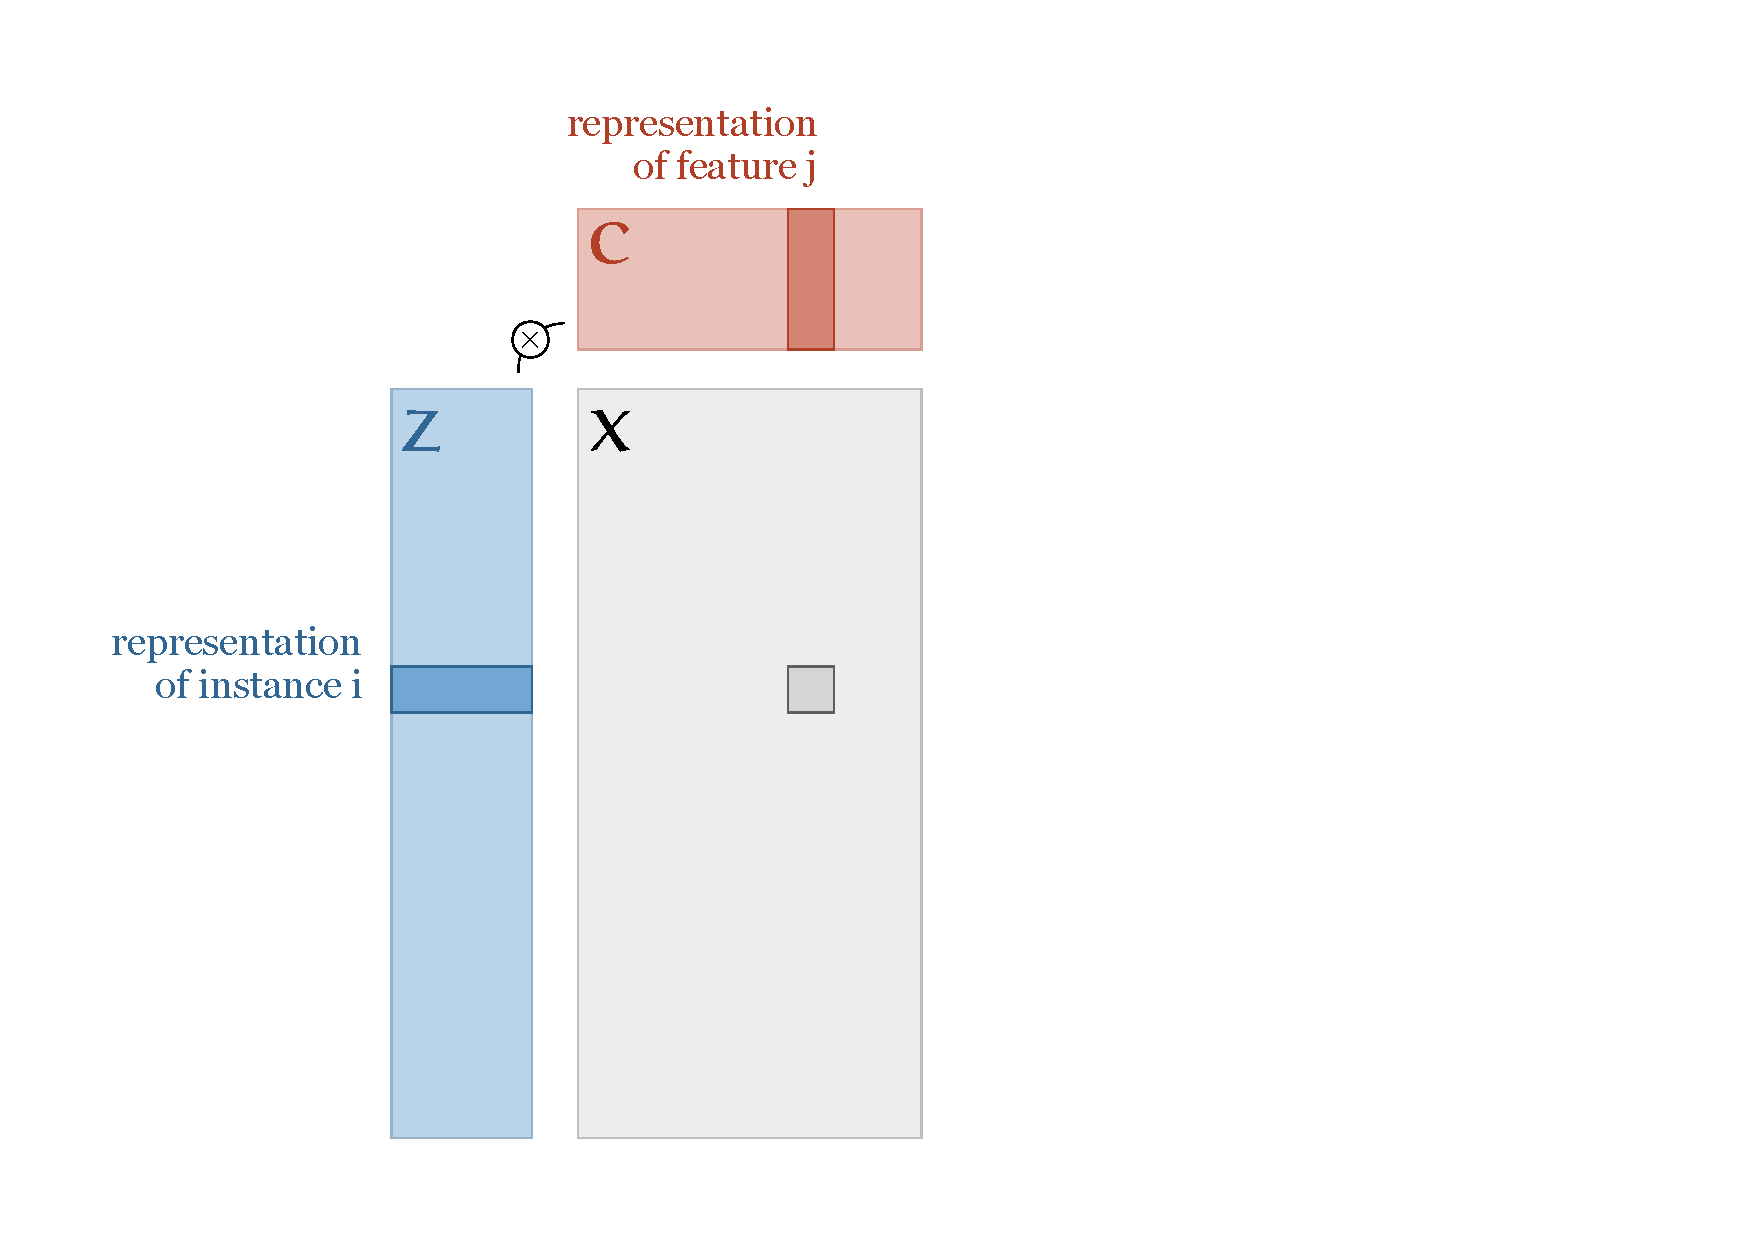
\includegraphics[width=0.5\textwidth]{./images/pca-4/pca-decomp.pdf}
	}
\end{figure}

%<figure class="narrow centering">
%<img src="/images/pca-4/pca-decomp.svg" class="half">
%</figure>

Here we see that PCA is nothing but a low-rank approximation of our data matrix \(\mbX\), albeit with the extra constraint that the columns of \(\bc{\mbZ}\) and \(\rc{\mbC}\) should be mutually orthogonal unit vectors.

One particularly useful aspect of this perspective is that it shows that we've already proved the Eckart-Young-Mirsky theorem.

In Chapter~\ref{chapter:eigenvectors}, we showed that PCA provides an optimal reconstruction from a lower dimensional representation, under the constraints that the reconstruction is linear and consists of orthogonal vectors.

First, note that the second constraint does not actually limit the quality of the solution. If we find a solution with non-orthogonal vectors, we can always convert them to an orthogonal set of vectors, keeping the reconstruction the same.

The conclusion is that if we have any matrix \(\gc{\mbM}\) and ask for a rank \(k\) approximation, we can interpret \(\gc{\mbM}\) as a data matrix and apply PCA. This will give us two matrices \(\bc{\mbZ}\) and \(\rc{\mbC}\) which we have already shown in previous chapters to be an optimal approximation to \(\gc{\mbM}\). As we already derived earlier, if we have a full SVD \(\gc{\mbM} = \rc{\mbU}\gc{\Sig}\rc{\mbV}^T\), then the PCA can be computed as \(\bc{\mbZ} = \rc{\mbU}\gc{\Sig}\) and \(\rc{\mbC} = \rc{\mbV}\).

\begin{aside}Earlier, we distributed  \(\gc{\Sig}\) equally over the two matrices. In PCA, it's more common to multiply it only by the principal components.
\end{aside}

So, Eckart-Young-Mirsky properly proved. However, we can do a little better. EYM doesn't say that the SVD solution is the \emph{only} optimal low-rank approximation to \(\gc{\mbM}\). There is a large set of solutions. What makes the SVD an especially useful member of this set is that it satisfies some extra requirements.

We've been here before with the PCA solution. We characterized the PCA objective originally as a reconstruction objective, and we noted that there we many solutions, even if we constrained them to be orthogonal. The PCA solution was special because even if we optimize for \(k\) principal components, the PCA solution is the one for which we can isolate the first \(r\) principal components and get a PCA solution for the problem with \(r\).

This is what makes the SVD unique among the solutions to the low rank approximation problem. A full SVD can be truncated at every \(k\) to give a solution to the rank \(k\) decomposition problem. A \(k\)-truncated SVD can be truncated at \(r < k\), to give a solution to the rank \(r\) problem. 

\begin{aside}There are some trivial variations, but apart from that, the singular values and their vectors are uniquely determined.	
\end{aside}

%<!-- It's illustrative to follow the proofs in detail, and to translate them to the SVD setting. We can start with the rank \(1\) decomposition. In that case, we are looking for two vectors \(\a\) and \(\b\) such that \(\a\b^T \spprox \gc{\M}\). If we add in scalars \(a\) and \(b\), then we can make the vectors unit vectors and require that \(\gc{\M} = rc{\u}\gc{\sigma}\rc{\v}^T\) with \(\a = a\rc{\u}\), \(\b = b\rc{v}\) and \(\gc{\sigma} = ab\).

%Our reconstruction objective now becomes

%\[
%\|\gc{\M} - \rc{\u}\gc{\sigma}\rc\|^2
%\] -->

What we can now do is take this as a \emph{definition} of the SVD. Then we can generalize to a definition for SVD under missing values. The first singular value \(\gc{\sigma}\), and its two singular vectors \(\rc{\mbu}\), \(\rc{\mbv}\), we choose in such a way that they minimize the reconstruction objective:

\index{Singular value decomposition!with missing values}

\[
\|\gc{\mbM} - \rc{\mbu}\gc{\sigma}\rc{\mbv}^T\| = \sum_{i,j} \left(\gc{M}_{ij} - \left(\rc{\mbu}\gc{\sigma}\rc{\mbv}^T \right)_{ij}\right)^2
\]

subject to the constraint that \(\rc{\mbu}\) and \(\rc{\mbv}\) are unit vectors. If some values of \(\gc{\mbM}\) are unknown, we sum only over the known values.

This is not how we defined first the singular vectors above. Instead, we looked for the unit vector that yielded the largest vector when multiplied by \(\gc{\mbM}\). This definition doesn't work with missing values, of course, because we can't compute the matrix multiplication unless all values of \(\gc{\mbM}\) are known. We know that the two definitions are equivalent, but only because we know that the SVD computes the PCA, and the first principal component can be defined this way.

If that feels like going the long way round, here is a more direct proof of the equivalence. We start with the reconstruction objective.

\begin{align*}
\argmin{\rc{\mbu}\; \rc{\mbv}\; \gc{\sigma}}\;\;&\|\gc{\mbM} - \rc{\mbu}\gc{\sigma}\rc{\mbv}^T\|^2 \\
\text{such that}\;\;& \|\rc{\mbu}\| = \|\rc{\mbv}\| = 1 \p \\
\end{align*}

Opening up the norm in the objective, we get

\begin{align*}
\|\gc{\mbM} - \rc{\mbu}\gc{\sigma}\rc{\mbv}^T\|^2 &= \sum_{ij} \left( \gc{M}_{ij} - \rc{u}_i\gc{\sigma}\rc{v}_j\right)^2\\
&= \sum_{i} \| \gc{\mbm}_i - \rc{u}_i\gc{\sigma}\rc{\mbv}\|^2
\end{align*}

where \(\gc{\mbm}_i\) is the \(i\)-th row of \(\gc{\mbM}\). If \(\gc{\mbM}\) is a data matrix, you can think of this as breaking up the reconstruction error over the whole matrix into a sum over the reconstruction error per instance.

Now, we apply the central trick that we first saw in Chapter~\ref{chapter:eigenvectors}: that reconstruction error is related to variance by the Pythagorean theorem (it always comes back to Pythagoras).

Looking at the following diagram

\begin{figure}[H]
	\centerline{
		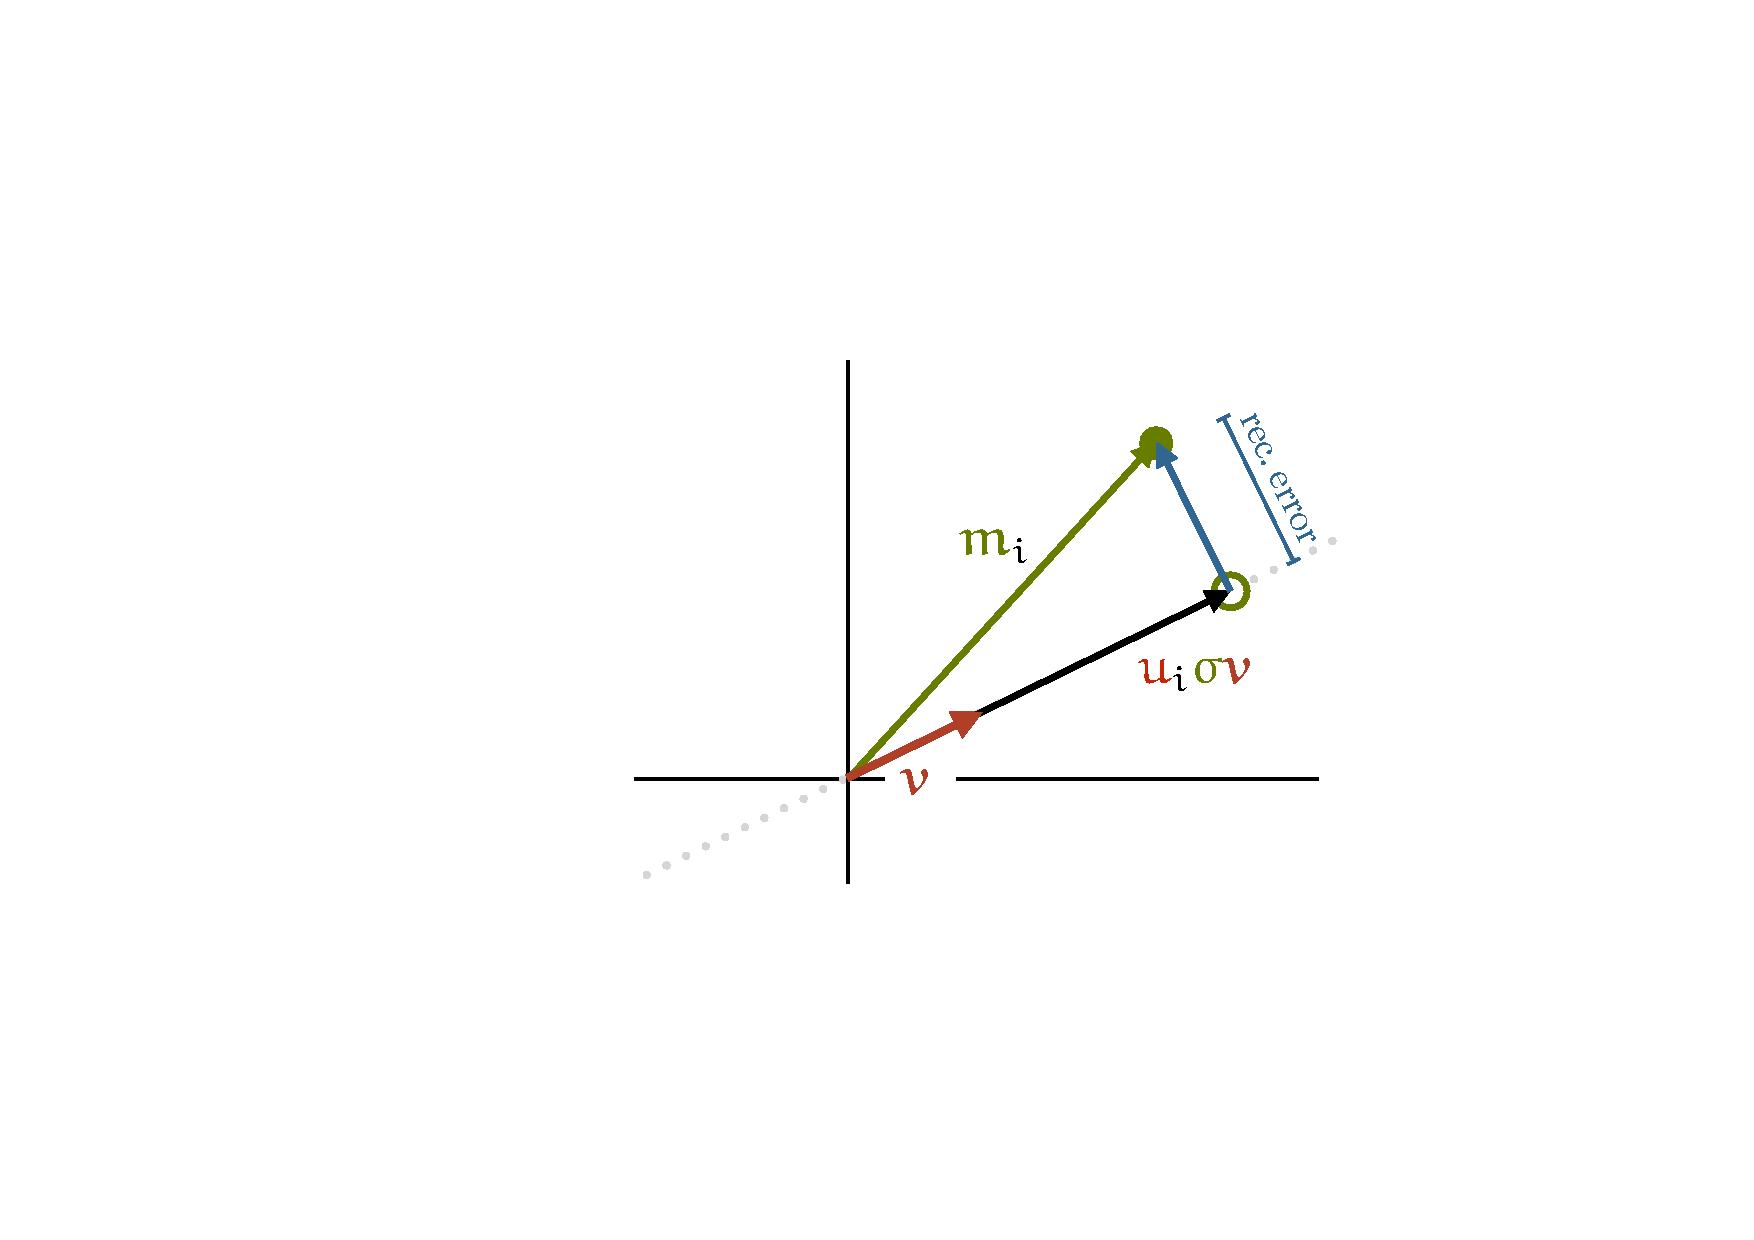
\includegraphics[width=0.8\textwidth]{./images/pca-4/pythagoras-again.pdf}
	}
	\caption*{The vectors \(\gc{\mbm}_i\) and \(\rc{u}_i\gc{\sigma}\rc{\mbv}\) form a right-handed triangle at the optimimum. However we set \(\rc{\mbv}\), \(\rc{u}_i\gc{\sigma}\rc{\mbv}\) will be an orthogonal projection of \(\gc{\mbm}_i\) onto \(\rc{\mbv}\) at the point where the reconstruction error is minimized. 
	}
\end{figure}

%<figure class="narrow centering">
%<img src="/images/pca-4/pythagoras-again.svg" class="half">
%<figcaption>The vectors \(\gc{\m}_i\) and \(\rc{u}_i\gc{\sigma}\rc{\v}\) form a right-handed triangle at the optimimum. However we set \(\rc{\v}\), \(\rc{u}_i\gc{\sigma}\rc{\v}\) will be an prtohogonal projection of \(\gc{\m}_i\) onto \(\rc{\v}\) at the point where the reconstruction error is minimized. 
%</figcaption>
%</figure>

we see that we have

\[ \|\gc{\mbm}_i\|^2 = \|\gc{\mbm}_i - \rc{u}_i\gc{\sigma}\rc{\mbv}\|^2 + \|\rc{u}_i\gc{\sigma}\rc{\mbv}\|^2\]

or, over all \(i\)

\[ \sum_i \|\gc{\mbm}_i\|^2 = \sum_i\|\gc{\mbm}_i - \rc{u}_i\gc{\sigma}\rc{\mbv}\|^2 + \sum_i \|\rc{u}_i\gc{\sigma}\rc{\mbv}\|^2\]

The left hand side is a constant, so minimizing one term on the right is equivalent to maximizing the other. With that, our objective \emph{becomes}

\begin{align*}
\argmax{\rc{\mbv}\; \rc{\mbu}\; \gc{\sigma}} & \sum_i \|\rc{u}_i\gc{\sigma}\rc{\mbv}\|^2 \\
\text{such that}\;\;& \|\rc{\mbu}\| = \|\rc{\mbv}\| = 1 \\
\end{align*}

Now, note that \(\rc{\mbv} = 1\), so that \(\|\rc{u}_i\gc{\sigma}\rc{\mbv}\|^2 = {\rc{u}_i}^2\gc{\sigma}^2\). This turns the objective into \(\sum_i {\rc{u}_i}^2\gc{\sigma}^2 = \gc{\sigma}^2\sum_i\rc{\mbu}_i = \gc{\sigma}^2\|\rc{\mbu}\|\), so that we get

\begin{align*}
\argmax{\rc{\mbv}\; \rc{\mbu}\; \gc{\sigma}}\;\;& \gc{\sigma}^2 \\
\text{such that}\;\;& \|\rc{\mbu}\| = \|\rc{\mbv}\| = 1 \\
\text{and}\;\;& \|\gc{\mbM}\rc{\mbv}\| = \gc{\sigma}\rc{\mbu}
\end{align*}

or, equivalently

\begin{align*}
\argmax{\rc{\mbv}}\;\;& \gc{\mbM}\rc{\mbv} \\
\text{such that}\;\;& \|\rc{\mbv}\| = 1 \p \\
\end{align*}

So, the reconstruction definition is equivalent to the ``maximum stretch'' definition for the first singular vector. The definition is the same for the other singular vectors, with the exception that there are additional constraints, so the same proof will work for the other singular vectors too.

We can now define an SVD for matrices that are only partially known, for instance, a recommendation matrix, or a data matrix with missing values. We simply use the reconstruction definition, and compute the reconstruction only over the known values.

\pagebreak\noindent The downside of this approach is that the problem is no longer easy to solve. The fast and robust algorithms that we have to compute SVDs for complete matrices don't work for incomplete ones. Instead we need to look to iterative approaches. There are a few options, but simple gradient descent is the simplest and probably the most popular. If we want a proper SVD, with the singular vectors separated and arranged by magnitude, we'll need to work them out iteratively. We search for the first singular vector, and once we've found it we search for the second singular vector orthogonal to it. This is like the iterative algorithm for PCA we introduced in Chapter~\ref{chapter:introduction}. It's slow, but we get a proper SVD with separated singular values.

If we don't want to wait that long, we can also solve the reconstruction problem in one go: find two orthogonal matrices \(\rc{\mbU}\)  and \(\rc{\mbV}\) and a diagonal matrix \(\gc{\Sig}\) so that their product approximates our matrix, all truncated to \(k\) dimensions. The downside, like the combined approach to solving the PCA problem, is that we don't get a neat separation of the singular vectors. If we truncate at \(k\), we can find a solution that is as good as the iterative solution, but the \(k\) vectors we find will be a mixture of the \(k\) vectors that the iterative algorithm returns.

%\section{Conclusion}

So that's the singular value decomposition. The workhorse of linear algebra.

In the context of PCA, you can think of the SVD as a way to compute a principal component analysis efficiently, but you can also think of it as an alternative definition. In Chapter~\ref{chapter:introduction}, we defined the PCA in term of minimizing reconstruction error, in Chapter~\ref{chapter:eigenvectors}, we defined it in terms of the eigenvectors of the covariance matrix, and here we have defined it a third time, in terms of the singular values of the data matrix. All of these definitions are, of course, equivalent, and all of them have different things to offer.

The main thing the SVD definition has to offer is that it is the preferred way to compute a principal component analysis. If you're willing to take an SVD routine as a given, you now have everything you need to compute the PCA in almost all settings. And in almost all cases, that is what you should do. There are very few situations where you would want to implement your own SVD algorithm.

Still, can we really claim to have understood SVD, and by extension PCA, if we cannot implement it from scratch? In the next chapter we will take the final step in our journey, and look at some algorithms for computing both eigenvectors and singular vectors.

%**Acknowledgements** Many thanks to Charlie Lu for corrections. 
%
%## Appendix

%
%
%
%<!--  -->
%
